%PREAMBLE
\begin{comment}
%\documentclass[11pt]{article}
%\newcommand{\pablo}[1]{\textcolor{blue}{{\bf  #1}}}
\newcommand{\carlos}[1]{\textcolor{red}{{\bf  #1}}}
\newcommand{\fabio}[1]{\textcolor{purple}{{\bf  #1}}}
\newcommand{\susana}[1]{\textcolor{violet}{{\bf  #1}}}

% HEP names :: https://ctan.javinator9889.com/macros/latex/contrib/hepnames/hepnames.pdf

\DeclarePairedDelimiter\bra{\langle}{\rvert}
\DeclarePairedDelimiter\ket{\lvert}{\rangle}
\DeclarePairedDelimiterX\braket[2]{\langle}{\rangle}{#1 \delimsize\vert #2}

\newcommand*{\yt}{\ensuremath{y_{t}}\xspace}
\newcommand*{\tchannel}{\ensuremath{t\text{-channel}}\xspace}
\newcommand*{\schannel}{\ensuremath{s\text{-channel}}\xspace}
%\newcommand*{\lepT}{\ensuremath{\Pl_{\Pt}}\xspace}
%\newcommand*{\lepH}{\ensuremath{\Pl_{\PHiggs}}\xspace}

%\newcommand*{\muR}{\ensuremath{\mu_{\text{R}}}\xspace}
%\newcommand*{\muF}{\ensuremath{\mu_{\text{F}}}\xspace}

% Add external packages
\usepackage[italic]{hepnicenames}

%%%%%%%%%%%%%%%%%%%%%%%
%  From NA-HIGG-2020-02-INT1-defs.sty    %
%%%%%%%%%%%%%%%%%%%%%%%
% Basic tHq-related macros
%\newcommand*{\tHq}{\ensuremath{\Pqt{}\PH{}\Pq}\xspace}
%\newcommand*{\tHq}{\ensuremath{\Ptop \PHiggs \Pq}\xspace}
%\newcommand*{\tHq}{\Pqt{}\PH{}\Pq}
\newcommand*{\tHq}{\ensuremath{tHq}\xspace}
\newcommand*{\tH}{\ensuremath{\Pqt{}\PH{}}\xspace}
\newcommand*{\tHqsec}{\texorpdfstring{\Pqt{}\PH{}\Pq}{tHq}}
\newcommand*{\tHqML}{\ensuremath{\Pqt{}\PH{}\Pq\,(\text{ML})}\xspace}
\newcommand*{\tHqbb}{\ensuremath{\Pqt{}\PH{}\Pq\,(\bbbar)}\xspace}
\newcommand*{\tbarHq}{\Paqt{}\PH{}Pq}
\newcommand*{\tHbb}{\ensuremath{\tHq (\PH \to \bbbar)}\xspace}
\newcommand*{\tHtautau}{\ensuremath{\tHq (\PH \to \Pgt{}\Pgt)}\xspace}
\newcommand*{\dR}{\ensuremath{\Delta R}\xspace}
\newcommand*{\trexfitter}{TRExFitter\xspace}
\newcommand*{\thqloop}{\texttt{tHqLoop}\xspace}


\newcommand*{\MpT}{\ensuremath{\vec{p}_{\text{T}}^{\text{miss}}}\xspace}
\newcommand*{\mtw}{\ensuremath{m_{\text{T}}(\Pl,\MET)}}
\newcommand*{\mlb}{\ensuremath{m_{\Pl\Pqb}}}
\newcommand*{\mOSSF}{\ensuremath{m_{\text{OSSF}}}\xspace}

% Background processes
\newcommand*{\ttX}{\ensuremath{\Pqt{}\Paqt{}X}\xspace}
\newcommand*{\tX}{\ensuremath{\Pqt{}X}\xspace}

%\newcommand*{\ttX}{\Pqt{}\Paqt{}+X}
\newcommand*{\ttH}{\Pqt{}\Paqt{}\PH}
%\newcommand*{\ttH}{\ensuremath{\Pqt{}\Paqt{}\PH}\xspace}
\newcommand*{\ttZ}{\Pqt{}\Paqt{}\PZ}
\newcommand*{\ttV}{\ensuremath{\Pqt{}\Paqt{}V}\xspace}
\newcommand*{\ttW}{\Pqt{}\Paqt{}\PW}
\newcommand*{\ttWj}{\ensuremath{t\bar{t}W+j}\xspace}
\newcommand*{\tZq}{\Pqt{}\PZ{}\Pq}
\newcommand*{\tWZ}{\Pqt{}\PW{}\PZ}
\newcommand*{\tWH}{\Pqt{}\PW{}\PH}
\newcommand*{\tHW}{\Pqt{}\PW{}\PH}
\newcommand*{\tW}{\Pqt{}\PW}
\newcommand*{\Wt}{\Pqt{}\PW}
\newcommand*{\diboson}{diboson\xspace}
\newcommand*{\Diboson}{Diboson\xspace}
\newcommand*{\triboson}{triboson\xspace}
\newcommand*{\Triboson}{Triboson\xspace}
\newcommand*{\Vjets}{\ensuremath{V\text{+\,jets}}\xspace}

\newcommand*{\ttt}{\ensuremath{ttt}\xspace}
\newcommand*{\tttt}{\ensuremath{t\bar{t}t\bar{t}}\xspace}
\newcommand*{\ggH}{\ensuremath{ggH}\xspace}
\newcommand*{\qqH}{\ensuremath{qqH}\xspace}
\newcommand*{\WH}{\ensuremath{WH}\xspace}
\newcommand*{\ZH}{\ensuremath{ZH}\xspace}

% Fake leptons
\newcommand*{\elHF}{\ensuremath{e_{\text{HF}}}\xspace}
\newcommand*{\muHF}{\ensuremath{\mu_{\text{HF}}}\xspace}
\newcommand*{\elCo}{\ensuremath{e_{\text{conv}}}\xspace} 
\newcommand*{\kelHF}{\ensuremath{\mu(e_{\text{HF}})}\xspace}
\newcommand*{\kmuHF}{\ensuremath{\mu(\mu_{\text{HF}})}\xspace}
\newcommand*{\kelCo}{\ensuremath{\mu(e_{\text{conv}})}\xspace} 

% Signal regions
\newcommand*{\dileptau}{\ensuremath{2\Pl+1\tauhad}\xspace}
\newcommand*{\dilepOStau}{\ensuremath{2\Pl\,\text{OS}+1\tauhad}\xspace}
\newcommand*{\dilepSStau}{\ensuremath{2\Pl\,\text{SS}+1\tauhad}\xspace}

\newcommand*{\onelep}{\ensuremath{1\Pl}\xspace}
\newcommand*{\dilep}{\ensuremath{2\Pl}\xspace}
\newcommand*{\dilepOS}{\ensuremath{2\Pl\,\text{OS}}\xspace}
\newcommand*{\dilepSS}{\ensuremath{2\Pl\,\text{SS}}\xspace}
%\newcommand*{\SS}{\ensuremath{\text{SS}}\xspace}
%\newcommand*{\OS}{\ensuremath{\text{OS}}\xspace}

\newcommand*{\trilep}{\ensuremath{3\Pl}\xspace}
\newcommand*{\lepditau}{\ensuremath{1\Pl+2\tauhad}\xspace}




\newcommand*{\lumi}{\ensuremath{\mathcal{L}}\xspace}
\newcommand*{\lumiunits}{$\,$ cm$^{2} \,$s$^{-1}$\xspace}


%Other
\newcommand*{\CM}{\ensuremath{\sqrt{s}}\xspace}
 
\newcommand*{\Wtb}{\ensuremath{tWb}\xspace}
\newcommand*{\tWb}{\Wtb}
%\newcommand*{\tWb}{\ensuremath{tWb}\xspace}
\newcommand*{\pfour}{\ensuremath{\boldsymbol{\textrm{p}}}\xspace} 

\newcommand*{\tchan}{\ensuremath{t}-channel}
\newcommand*{\mtop}{\ensuremath{m_{\Ptop}}\xspace}
%\newcommand*{\mH}{\ensuremath{m_H}\xspace}
%\newcommand*{\HT}{\ensuremath{H_{\text{T}}}\xspace}

%\newcommand*{\PWplus}{\ensuremath{\PW^{+}}\xspace}
%\newcommand*{\PWminus}{\ensuremath{\PW^{-}}\xspace}
%\newcommand*{\Pgamma}{\ensuremath{\gamma}\xspace}

 \newcommand*{\greekphys}{\ensuremath{\varphi\upsilon\sigma\iota\kappa \eta}\xspace}
 \newcommand*{\greekatom}{\ensuremath{\alpha \tau o \mu o \nu}\xspace}
 \newcommand{\emu}{\ensuremath{\Pe/\Pmu}\xspace}

\newcommand*{\momentum}{\ensuremath{\overrightarrow{p}}\xspace} 
%\newcommand*{\CP}{\ensuremath{\mathcal{CP}}\xspace}
\newcommand*{\CP}{CP\xspace}

% Decays (Please, check latex/atlasprocess.sty and latex/atlasparticle.sty for more definitions!)
\newcommand{\bb}{\ensuremath{\Pqb\Paqp}\xspace}
\newcommand{\WW}{\ensuremath{\PW\PW^{*}}\xspace}
\newcommand{\ZZ}{\ensuremath{\PZ\PZ^{*}}\xspace}
\newcommand{\Higgsdecays}{\ensuremath{\PH \rightarrow b\bar{b}, \WW, \ZZ, \tau\tau}\xspace}
\newcommand{\Higgsdecayslep}{\ensuremath{\PH \rightarrow \WW, \ZZ, \tau\tau}\xspace}
\newcommand{\HWW}{\ensuremath{\PH \rightarrow \WW}\xspace}
\newcommand{\HZZ}{\ensuremath{\PH \rightarrow \ZZ}\xspace}

% reconstruction definitions
\newcommand{\pnutop}{\ensuremath{\vec{p^{\Pnu, \text{top}}}}\xspace}
\newcommand{\pnutopx}{\ensuremath{p^{\Pnu, \text{top}}_x}\xspace}
\newcommand{\pnutopy}{\ensuremath{p^{\Pnu, \text{top}}_y}\xspace}
\newcommand{\pnutopz}{\ensuremath{p_{z}(\Pnu_{\text{top}})}\xspace}
\newcommand{\pnutopT}{\ensuremath{\pT(\Pnu_{\text{top}})}\xspace}
\newcommand{\phinutop}{\ensuremath{\phi(\Pnu_{\text{top}})}\xspace}
\newcommand{\pltop}{\ensuremath{\vec{p^{\Plepton, \text{top}}}}\xspace}
\newcommand{\pltopx}{\ensuremath{p^{\Plepton, \text{top}}_x}\xspace}
\newcommand{\pltopy}{\ensuremath{p^{\Plepton, \text{top}}_y}\xspace}
\newcommand{\pltopz}{\ensuremath{p^{\Plepton, \text{top}}_z}\xspace}
\newcommand{\pltopT}{\ensuremath{\pT(\Plepton_{\text{top}})}\xspace}
\newcommand{\philtop}{\ensuremath{\phi(\ell_{\text{top}})}\xspace}
\newcommand{\phibtop}{\ensuremath{\phi(b_{\text{top}})}\xspace}
\newcommand{\tauvis}{\ensuremath{\Ptau_{\text{vis}}}\xspace}

\newcommand{\leptop}{\ensuremath{\Plepton^{\text{top}}}\xspace}
\newcommand{\lepH}{\ensuremath{{\Plepton^{\PH}}}\xspace}
\newcommand{\Hvismass}{\ensuremath{m_{\PH}^{\text{vis}}}\xspace}
\newcommand{\toprecomass}{\ensuremath{\mtop^{\text{reco}}}\xspace}
% \newcommand{\toprecomass}{\ensuremath{\Pqt_{\text{reco}}^{\text{m}}\xspace}}
% \newcommand{\Hvismass}{\ensuremath{\PH_{\text{vis}}^{\text{m}}\xspace}}
\newcommand{\MMC}{\texttt{MissingMassCalculator}\xspace}

% luminosity (2015)
\newcommand{\lumiFifteenRelUnc}{1.13} % in [%]
\newcommand{\lumitagFifteen}{{\small\texttt{OfLumi-13TeV-008}}}
%\newcommand{\lumiFifteenInPbNoUnits}{3219.56}
%\newcommand{\lumiFifteenInFbNoUnits}{3.2}
\newcommand{\lumiFifteenInPbNoUnits}{3244.54} % final luminosity recommendation for Run 2 analyses (https://twiki.cern.ch/twiki/bin/viewauth/Atlas/LuminosityForPhysics#2015_2018_13_TeV_proton_proton_f)
\newcommand{\lumiFifteenInFbNoUnits}{3.2}
%\newcommand{\dataperiodsFifteen}{D--J}
\newcommand{\dataperiodsFifteen}{D--H,J}
\newcommand{\firstdatarunFifteen}{276262}
\newcommand{\lastdatarunFifteen}{284484}
\newcommand{\datarunsFifteen}{\firstdatarunFifteen--\lastdatarunFifteen}
\newcommand{\dataeventsFifteen}{220.58M}

% luminosity (2016)
\newcommand{\lumiSixteenRelUnc}{0.89} % in [%]
\newcommand{\lumitagSixteen}{{\small\texttt{OfLumi-13TeV-009}}}
%\newcommand{\lumiSixteenInPbNoUnits}{32988.1}
%\newcommand{\lumiSixteenInFbNoUnits}{33.0}
% final luminosity recommendation for Run 2 analyses (https://twiki.cern.ch/twiki/bin/viewauth/Atlas/LuminosityForPhysics#2015_2018_13_TeV_proton_proton_f)
\newcommand{\lumiSixteenInPbNoUnits}{33402.2}
\newcommand{\lumiSixteenInFbNoUnits}{33.4}
%\newcommand{\dataperiodsSixteen}{A--L}
\newcommand{\dataperiodsSixteen}{A--G,I,K,L}
\newcommand{\firstdatarunSixteen}{297730}
\newcommand{\lastdatarunSixteen}{311481}
\newcommand{\datarunsSixteen}{\firstdatarunSixteen--\lastdatarunSixteen}
\newcommand{\dataeventsSixteen}{1057.84M}

% luminosity (2017)
\newcommand{\lumiSeventeenRelUnc}{1.13} % in [%]
\newcommand{\lumitagSeventeen}{{\small\texttt{OfLumi-13TeV-010}}}
%\newcommand{\lumiSeventeenInPbNoUnits}{44307.4}
%\newcommand{\lumiSeventeenInFbNoUnits}{44.3}
% final luminosity recommendation for Run 2 analyses (https://twiki.cern.ch/twiki/bin/viewauth/Atlas/LuminosityForPhysics#2015_2018_13_TeV_proton_proton_f)
\newcommand{\lumiSeventeenInPbNoUnits}{44630.6}
\newcommand{\lumiSeventeenInFbNoUnits}{44.6} 
%\newcommand{\dataperiodsSeventeen}{B--K}
\newcommand{\dataperiodsSeventeen}{B--F,H,I,K}
\newcommand{\firstdatarunSeventeen}{325713}
\newcommand{\lastdatarunSeventeen}{340453}
\newcommand{\datarunsSeventeen}{\firstdatarunSeventeen--\lastdatarunSeventeen}
%%%\newcommand{\datarunsSeventeen}{324320--341649}
\newcommand{\dataeventsSeventeen}{1340.80M}

% luminosity (2018)
\newcommand{\lumiEightteenRelUnc}{1.10} % in [%]
\newcommand{\lumitagEightteen}{{\small\texttt{OfLumi-13TeV-010}}}
%\newcommand{\lumiEightteenInPbNoUnits}{58450.1}
%\newcommand{\lumiEightteenInFbNoUnits}{58.5}
% final luminosity recommendation for Run 2 analyses (https://twiki.cern.ch/twiki/bin/viewauth/Atlas/LuminosityForPhysics#2015_2018_13_TeV_proton_proton_f)
\newcommand{\lumiEightteenInPbNoUnits}{58791.6}
\newcommand{\lumiEightteenInFbNoUnits}{58.8}
\newcommand{\lumiEightteenInPb}{\SI{\lumiEightteenInPbNoUnits}{\per\pb}}
\newcommand{\lumiEightteenInFb}{\SI{\lumiEightteenInFbNoUnits}{\per\fb}}
%\newcommand{\dataperiodsEightteen}{B--Q}
\newcommand{\dataperiodsEightteen}{B--D,F,I,K,L,M,O,Q}
\newcommand{\firstdataruEightteen}{348885}
\newcommand{\lastdatarunEightteen}{364292}
\newcommand{\datarunsEightteen}{\firstdataruEightteen--\lastdatarunEightteen}
%%%\newcommand{\datarunsEightteen}{348197--364292}
\newcommand{\dataeventsEightteen}{1716.77M}

% luminosity (2015+2016+2017)
%\newcommand{\lumiInPb}{80515.06~\invpb}
% \newcommand{\partlumi}{\SI{80.52}{\per\fb}}
%\newcommand{\datafirstyear}{2015}
%\newcommand{\datalastyear}{2017}

% luminosity (2015+2016+2017+2018)
%
% https://twiki.cern.ch/twiki/bin/viewauth/Atlas/LuminosityForPhysics#2015_2018_13_TeV_proton_proton_f
% final luminosity recommendation for Run 2 analyses (central value + uncertainty)
\newcommand{\lumiRelUnc}{0.83} % in [%]
\newcommand{\lumiInPbNoUnits}{140068.94} % in pb-1
\newcommand{\lumiInFbNoUnits}{140} % in fb-1
\newcommand{\lumiWithUnc}{\ensuremath{140.1 \pm 1.2}\,\si{\per\fb}} % in fb-1
%
% old recommendation
%\newcommand{\lumiRelUnc}{1.7} % in [%]
%\newcommand{\lumiInPbNoUnits}{138965.16} % in pb-1
%\newcommand{\lumiInFbNoUnits}{139} % in fb-1
%\newcommand{\lumiWithUnc}{\ensuremath{\lumiInFbNoUnits \pm 2.4}\,\si{\per\fb}} % in fb-1
\newcommand{\dataeventsAll}{4335.99M}
%
\newcommand{\lumiInPb}{\SI{\lumiInPbNoUnits}{\per\pb}}
%\newcommand{\lumi}{\SI{\lumiInFbNoUnits}{\per\fb}}
\newcommand{\datafirstyear}{2015}
\newcommand{\datalastyear}{2018}

% % tunes and PDF sets
\def\cteq{CTEQ6L1\xspace}
\def\ctten{CT10\xspace}
\def\cttennlo{CT10\,NLO\xspace}
\def\cttennnlo{CT10\,NNLO\xspace}
\def\ctfourteennlo{CT14\,NLO\xspace}
\def\ctfourteennnlo{CT14\,NNLO\xspace}
\def\nnpdfnnlo{NNPDF3.0\,NNLO\xspace}
\def\nnpdfnlofourflav{NNPDF3.0\,NLO\,nf4\xspace}
\def\nnpdfnlo{NNPDF3.0\,NLO\xspace}
\def\nnpdftwonlo{NNPDF2.3\,NLO\xspace}
\def\nnpdftwo{NNPDF2.3\,LO\xspace}
\def\nnpdftwofiveflav{NNPDF2.3\,5f\,FFN\xspace}
\def\mstw{MSTW2008\,NLO\xspace}
\def\a14{A14\xspace}
\def\auet{AUET2\xspace}
\def\aznlo{AZNLO\xspace}
\def\mmhtnnlo{MMHT2014\,NNLO\xspace}
\def\mmhtnlo{MMHT2014\,NLO\xspace}
\def\mmhtlo{MMHT2014\,LO\xspace}
\def\mstwnlo{MSTW2008\,68\%\,CL\,NLO \xspace}
\def\mstwnnloninety{MSTW2008\,90\%\,CL\,NNLO \xspace}
\def\ueee{UE-EE-5\xspace}




 
\endinput


\begin{document}
%ENDPREAMBLE
\end{comment}


\chapter{The Standard Model of particle physics}
\label{chap:Introduction}
%{\LARGE \textbf{Theoretical framework}\\}

%\tableofcontents

%\vspace*{0.1 cm} 
%\hspace*{200pt} \\
%\hspace*{175pt} \textit{L’essentiel est invisible pour les yeux.} \\
%\hspace*{175pt} ---\textsc{Antoine de Saint-Exupéry,} \\% \textit{} \\
%\hspace*{200 pt}     \textsc{Le Petit Prince (1943)} \\% \textit{} \\
%\vspace*{2cm} 

\vspace*{0.1 cm} 
\hspace*{200pt} \\
\hspace*{120pt} \textit{Tot el que sentireu en aquest programa ha passat.} \\
\hspace*{120pt} \textit{[...] En algunes descripcions aquest programa} \\
\hspace*{120pt} \textit{podria ferir sensibilitats. [...] Començem!} \\
\hspace*{205pt} ---\textsc{Carles Porta,} \\% \textit{} \\
\hspace*{240 pt}     \textsc{Crims (2020)} \\% \textit{} \\
\vspace*{2cm} 


%The Standard Model of particle physics (SM) is a theoretical framework that describes 
%the fundamental particles and their interactions via three of the four fundamental forces 
%of nature (excluding gravity). It is considered one of the most successful and extensively 
%tested theories in physics, explaining the behaviour of subatomic particles and their interactions 
%with one another. In this chapter the basics of the SM are described by presenting 
%in Section~\ref{sec:chap1:SM_and_EParticles} the particles that compose it. 
%The three fundamental forces are described in Sections \ref{sec:chap1:QED}, \ref{sec:chap1:EW}
%and \ref{sec:chap1:QCD}. The Section~\ref{sec:chap1:ParticleMasses} presents the
%mechanism that provides masses to the fundamental particles. 
%Finally, the limitations of the SM are presented in Section~\ref{sec:chap1:Wrapup}.

%%%%%%%%%%%%%%%%%%%%%%%
%  The Standard Model of particle physics   %
%%%%%%%%%%%%%%%%%%%%%%%
%\section{The Standard Model of particle physics}
%\label{sec:chap1:TheSM}
Since the very first moment of our history, humankind has pursued the knowledge of nature
and has tried to understand and describe how the universe works at a fundamental level. 
In fact, the word \textit{physics} comes from the Greek word ``\greekphys'' which means 
``nature''~\cite{etymology_web, Greek_web}.
Most of the enquires regarding this, can be boiled down to two basic questions:
what are the ultimate building blocks of reality? and which are the rules that govern them?

In the 7$^{th}$ century BCE, the pre-Socratic philosopher Thales of Miletus already proclaimed that every 
event had a natural cause~\cite{Singer_C}. Later, to understand how the basic components of the matter were
formed, the ancient Indian philosophers such as Kaṇāda 
\cite{leaman2002key} in the 6$^{th}$ century BCE
and Greeks Democritus and Leucippus~\cite{taylor2010atomists} in the 5$^{th}$ century BCE developed the atomism,
which comes from ``\greekatom'' meaning uncuttable or indivisible.


%In the middle ages the atomism was mainly abandoned although some thinkers such as
%Dignāga and Dharmakirti~\cite{nakamura1980indianbuddhism} in the 5$^{th}$ century CE and 
%the islamic philosopher al-Ghazali in the 11$^{th}$, kept discussing it. The abandonement
%lasted until the 17$^{th}$ century,
%when a renewed interest arose in Epicurean atomism and corpuscularianism. Some 
%of the most notable figures are René Descartes and Robert Boyle.
%Corpuscularianism is similar to atomism, except that where atoms were supposed 
%to be indivisible, corpuscles could in principle be divided.

%A renewed interest in atomism and corpuscularianism arose in the 17$^{th}$ century
%with notable contributions by I. Newton~\cite{newman2010newton} and R. Boyle~\cite{boyle1667origin}.
%By the early 19th century, the useful practices of engineering and technology began to 
%influence philosophical explanations for the composition of matter. 
%Empirical evidence on the composition of matter was found by
%J. Dalton~\cite{dalton1808newsystem}


% Thales :: 7th BCE
% Democritus and Leucippus :: 5th BCE
% Kaṇāda :: 6th-2nd BCE <- El newton indio
% Dignāga and Dharmakirti :: 5th CE 
% al-Ghazali :: 11th
% Descartes :: 16th
% Robert Boyle  : 17th
% Newton :: 17th <- Light as a corpuscule 
% Lavoisier :: Late 18th
% Dalton :: 1808
% Brwon :: 1827 <- Brwonian motion
% Thompson :: 1897 <- Electron
% Einstein :: 1905
% Perrin :: 1908
% Rutherford :: 1912 <- Nucleous
% Soddy :: 1913 <- Periodic Table
% Bohr :: 1913
% Heisenberg :: 1925 <-  Mathematical formulation of quantum mechanics
% Schrödinger :: 1925 
% Chadwick :: 1932 <- Proton
% Hahn, Meitner :: 1938 <- Nuclear fission
% 1950 :: Accelerators


From then to our days, the search for the minute fragments that comprise the matter and its interactions has led us to the
 Standard Model of particle physics (SM), one of the most successful scientific theories cultivated so far. This understanding
of the universe can explain phenomena from the behaviour of atoms to how stars burn. 


%\begin{align*}
%\mathcal{L} &= - \frac{1}{4} F_{\mu \nu} F^{\mu \nu} \\
%   &\phantom{{}=}+ i \bar{\psi} \cancel{D} \psi + h.c. \\
%    &\phantom{{}=}+ \bar{\psi}_i y_{ij} \psi_j \phi + h.c. \\
%    &\phantom{{}=}+ |D_\mu \phi|^2 - V(\phi)
%\end{align*}

In this chapter, the basics of the SM are described by presenting 
in Section~\ref{sec:chap1:SM_and_EParticles} the particles that compose it. 
The three fundamental forces are described in Sections \ref{sec:chap1:QED}, \ref{sec:chap1:EW}
and \ref{sec:chap1:QCD}. Section~\ref{sec:chap1:ParticleMasses} presents the
mechanism that provides masses to the fundamental particles. 
Finally, the limitations of the SM are presented in Section~\ref{sec:chap1:Wrapup}.

\section{Introduction}
\label{sec:chap1:SM_and_EParticles}
Based on the Quantum Field Theory (QFT), the SM of particle physics provides the theoretical framework that constitutes what is 
currently accepted as the best description of particle physics. It aims to explain both all particles of matter and
 their interactions. The completion of the SM was a collaborative effort of several scientists during the second half of the
$20^\text{th}$ century, being the current formulation finalised in the decade of 1970s. A representation of the fundamental particles 
%, i.e. particles that are not made of anything else, 
that compose the SM is presented in Figure~\ref{fig:Chap1:SM}.
%Most of these particles are unstable and decay to lighter particles within fractions of a second. 
% Maybe some comment about the fact that decaying to something doesn't mean to be made of that thing. 
 As the scheme in Figure~\ref{fig:Chap1:SM} indicates, the 
12 fermions have their corresponding 12 anti-fermions-

 and the quarks and gluons carry colour charge. 
\begin{figure}
    \centering
    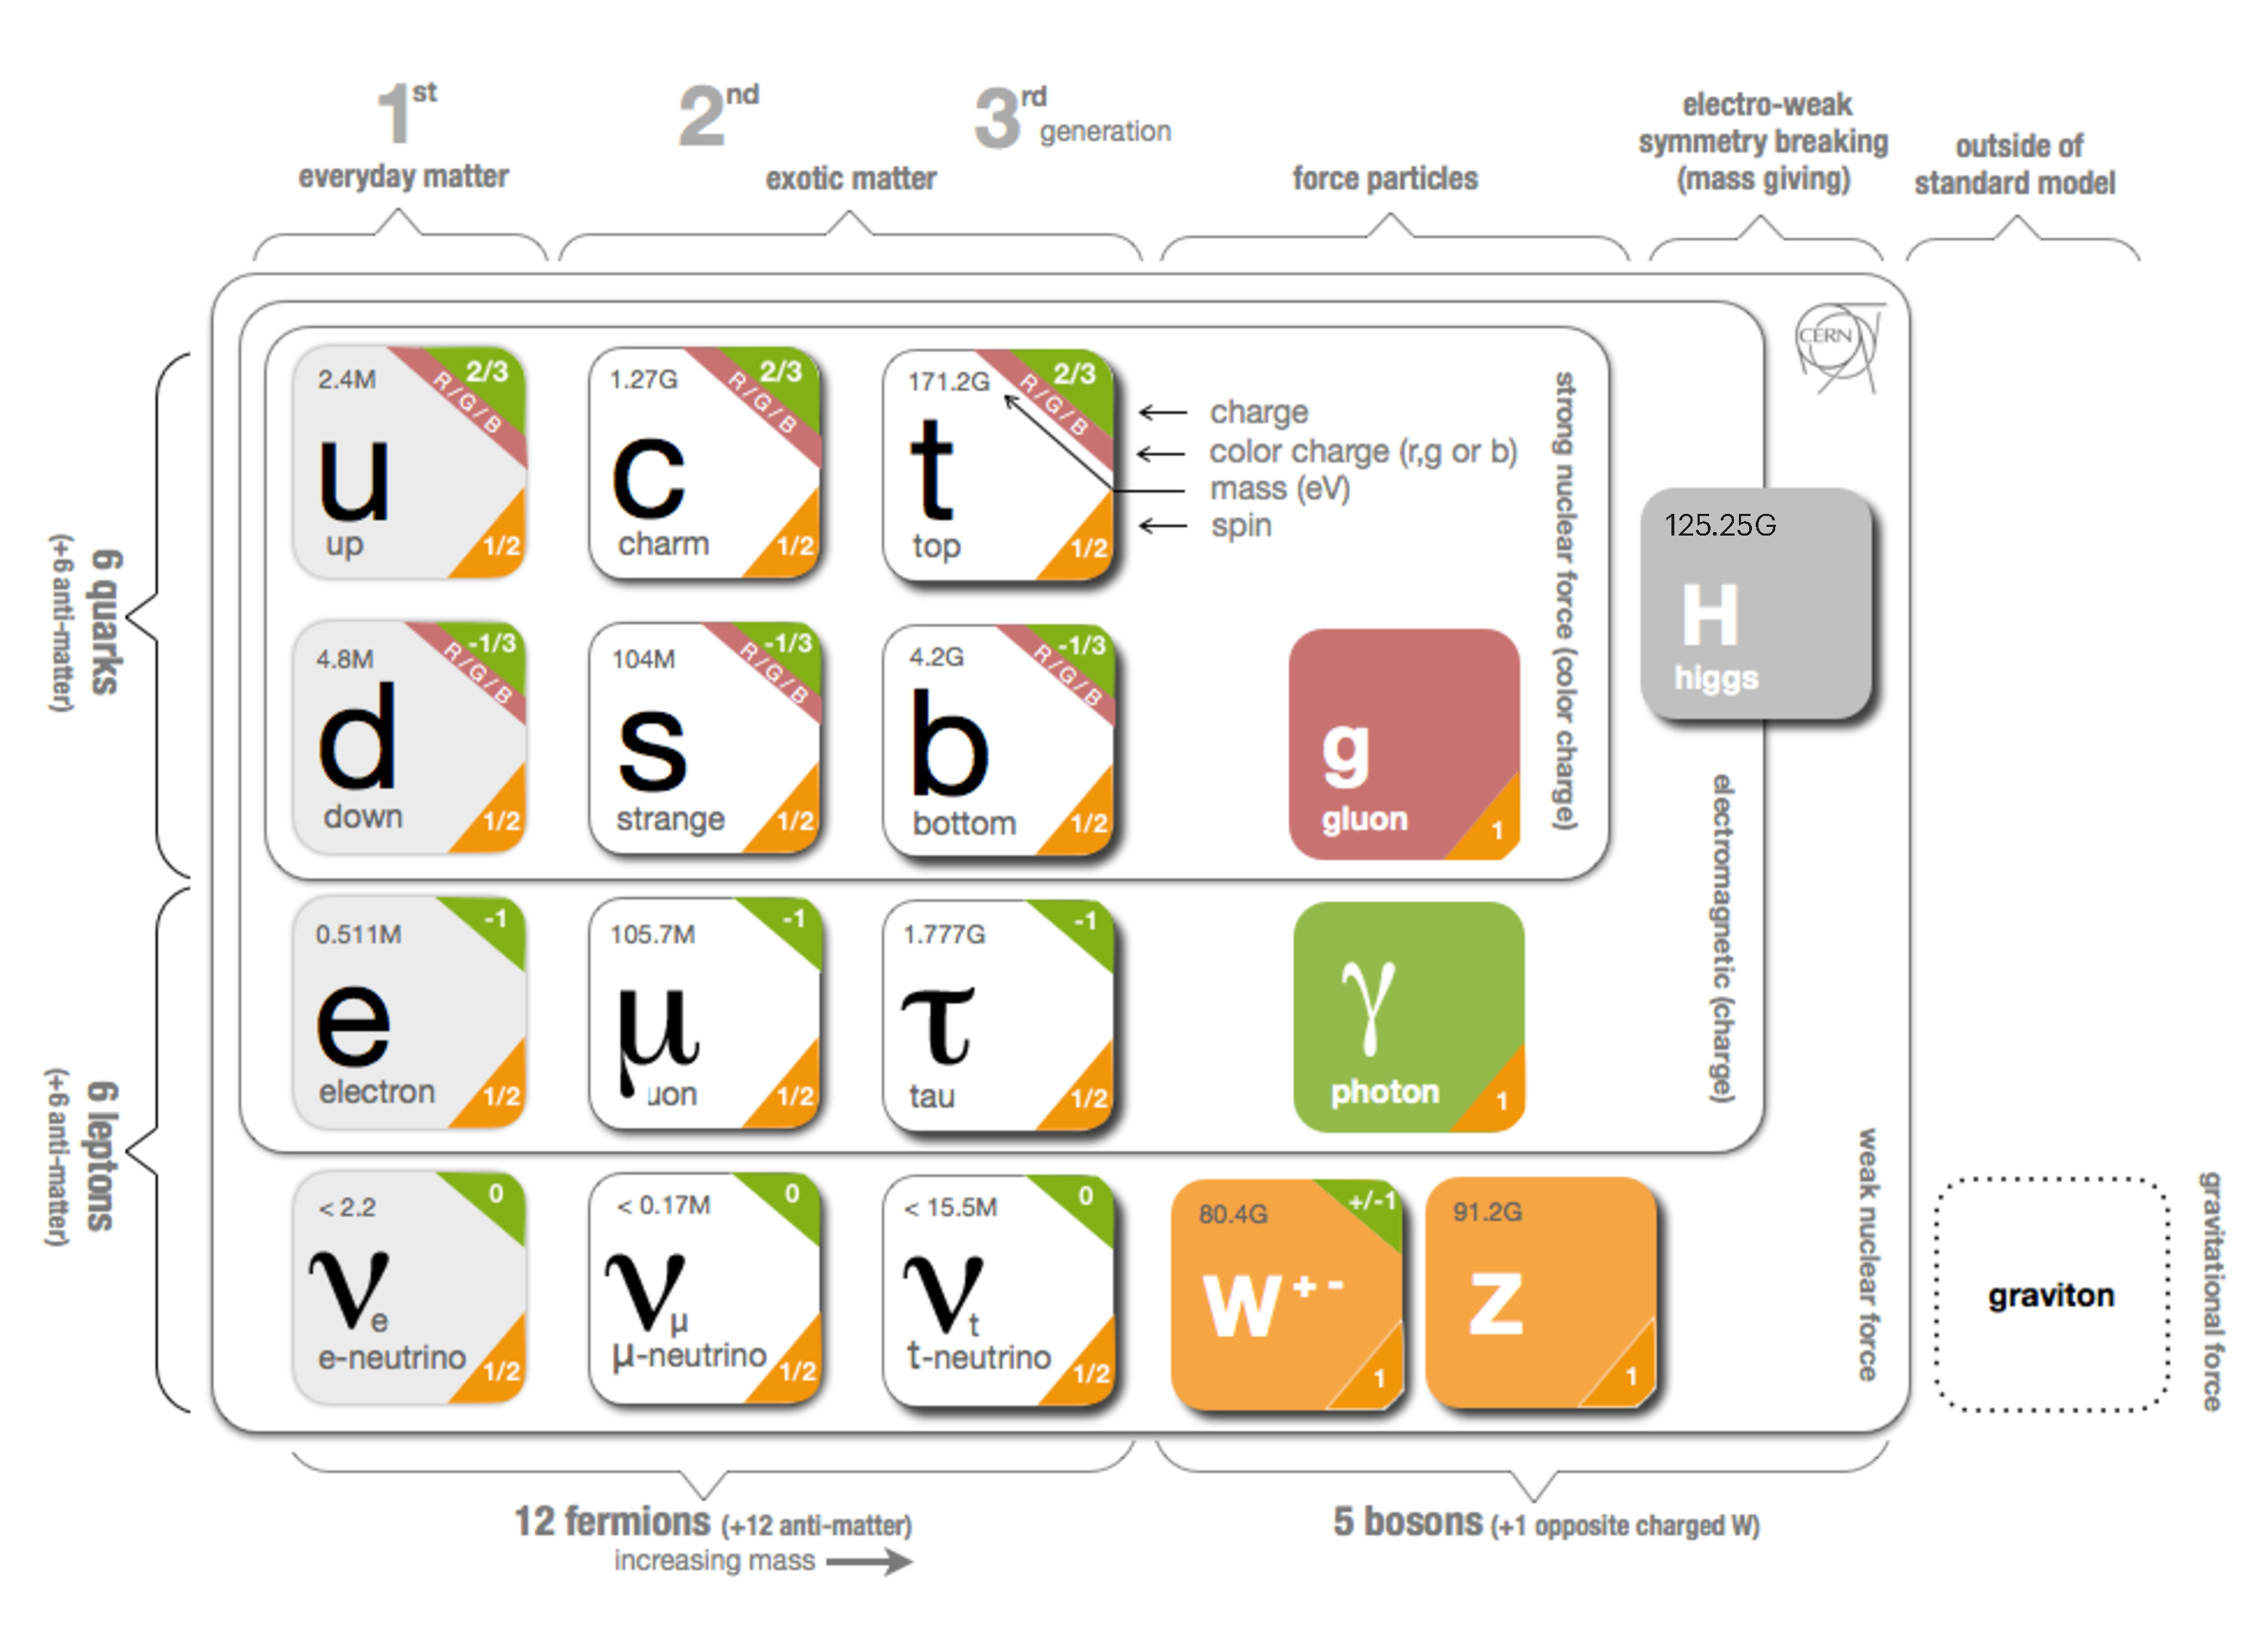
\includegraphics[width = 1\textwidth]{Chapter1/SMofElementaryParticles_fancy_modified}
    \caption{Fundamental particles of the SM (image taken and then modified from Reference~\cite{Purcell:1473657}). }
    % In each box the upper-left corner express the mass in eV, the upper-right the electric charge (green) and possible colour charges (red), and the lower-right the spin.}
    \label{fig:Chap1:SM}
\end{figure}




The SM is a gauge theory based on the symmetry group $SU(3)_\text{C} \bigotimes SU(2)_{\text{L}} \bigotimes U(1)_{\text{Y}}$, which
describes all fundamental interactions except the gravitational force\footnote{The gravitational interaction is described by Einstein's General Relativity (GR)~\cite{Einstein:1916vd}.}.
This theory provides a description for the strong, weak and electromagnetic interactions via the exchange of the corresponding
vector\footnote{``Vector bosons'' refer to all particles that have spin 1 in contrast to the ``scalar bosons'' which have spin 0.} bosons (spin-1 gauge fields).
The mediation for the electromagnetic interaction (explained in Section~\ref{sec:chap1:QED}) 
is done by one massless photon (\Pgamma).  This force is invariant under the $U(1)$ symmetry group.
While for the weak interaction, guided by $SU(2)$, three massive bosons,
\PWplus, \PWminus and \PZ, act as mediators (with masses 
$m_{\PWpm}= 80.385 \pm 0.015$~GeV~\cite{ATLAS:2017rzl} and 
$m_{\PZ}=  91.1876 \pm 0.0021$~GeV~\cite{ALEPH:2005ab}). 
Although the electromagnetic and weak interactions seem completely different at low energies, they are two aspects of the same force and
can be described simultaneously by the $SU(2)_\text{L} \bigotimes U(1)_\text{Y}$ 
symmetry group, which represents the so called electro-weak (EW) sector (detailed in Section~\ref{sec:chap1:EW}).
The strong force, with its eight massless gluons (\Pgluon), is described by the $SU(3)_\text{C}$ colour group (see Section~\ref{sec:chap1:QCD}). 
All these interactions differ in their magnitude, range and the physical phenomena that they describe. These features
are summarised in Table~\ref{tab:Chap1:FundamentalInteractions}, where 
not only the interactions described by the SM are included but the
gravitation is shown as well for completeness.  

Apart from the vector bosons, there is one massive scalar boson, the
 Higgs boson (with mass $\mH = 125.25\pm0.17$~GeV~\cite{Workman:2022ynf}). %~\cite{pdgHiggs}
Through the interaction with this particle, all massive particles of Figure 
\ref{fig:Chap1:SM} gain their masses via the EW spontaneous symmetry breaking.
This mechanism was first described by F. Englert, R. Brout~\cite{PhysRevLett.13.321} 
and P.W. Higgs~\cite{PhysRevLett.13.508}, and it is summarised in Section 
\ref{sec:chap1:ParticleMasses:HiggsMechanism}. 
% Gauge theory: A type of field theory in which the Lagrangian (and hence the dynamics of the system itself) does not 
% change (is invariant) under local transformations according to certain smooth families of operations 

\begin{table}[]
\centering
\begin{tabular}{l c c c c c}
\toprule
%Interaction & \begin{tabular}[c]{@{}l@{}}Mediator\\ boson\end{tabular} & Theory & \begin{tabular}[c]{@{}l@{}}Relative \\ stregth\end{tabular} & Range (m) \\ \midrule
Interaction     		& Theory  			& Mediator             	& Relative strength 	& Range (m) 	\\ \midrule
Strong          		& QCD	 		& $\Pgluon$              	& 1                		& $10^{-15}$    \\
Electromagnetic 	& QED/EW 		& $\Pgamma$          	&  1/137                	& $\infty$         	\\
Weak            		& EW   			& $\PWpm$, $\PZ$	&  $10^{-6}$              & $10^{18}$      \\
Gravitational     		& GR       			& -		 		&  $6\times10^{-39}$	& $\infty$  	\\ \bottomrule          
\end{tabular}
\caption{Typical strength of the fundamental interactions with respect to the strong interaction. Here the strength is understood as the coupling constant or gauge coupling parameter. 
%The description of the electromagnetism and weak interactions is unified by the EW interaction.
In GR the gravitational interaction is not a force but the effect of the four-dimensional spacetime curvature and, hence, it has no mediator in this formalism.}
\label{tab:Chap1:FundamentalInteractions}
\end{table}


%There are two important and distinct SU(3) symmetries that are relevant for the strong interactions: 
%SU(3) colour symmetry of the quark and gluon dynamics and SU(3) flavour symmetry of light quarks. 
%Each of these symmetries refers to an underlying threefold symmetry in strong interaction physics.

%A representation of the fundamental particles that compose the SM is presented in Figure~\ref{fig:Chap1:SM}.
%It is necessary to take into account that all quarks and leptons have their analogous antiparticles.% and 
% that the quarks and gluons carry the colour charge\footnote{Antiquarks carry the anti  charge}. Therefore, a more complete illustration
%of the complete set of fundamental is displayed in Figure~\ref{fig:Chap1:SM_color}, where appear the colour variations and the antiparticles
%for all the particles in Figure~\ref{fig:Chap1:SM}. The origin of the colour charge is discussed in Section~\ref{sec:chap1:QCD}.

%\begin{figure}
%    \centeringring
%   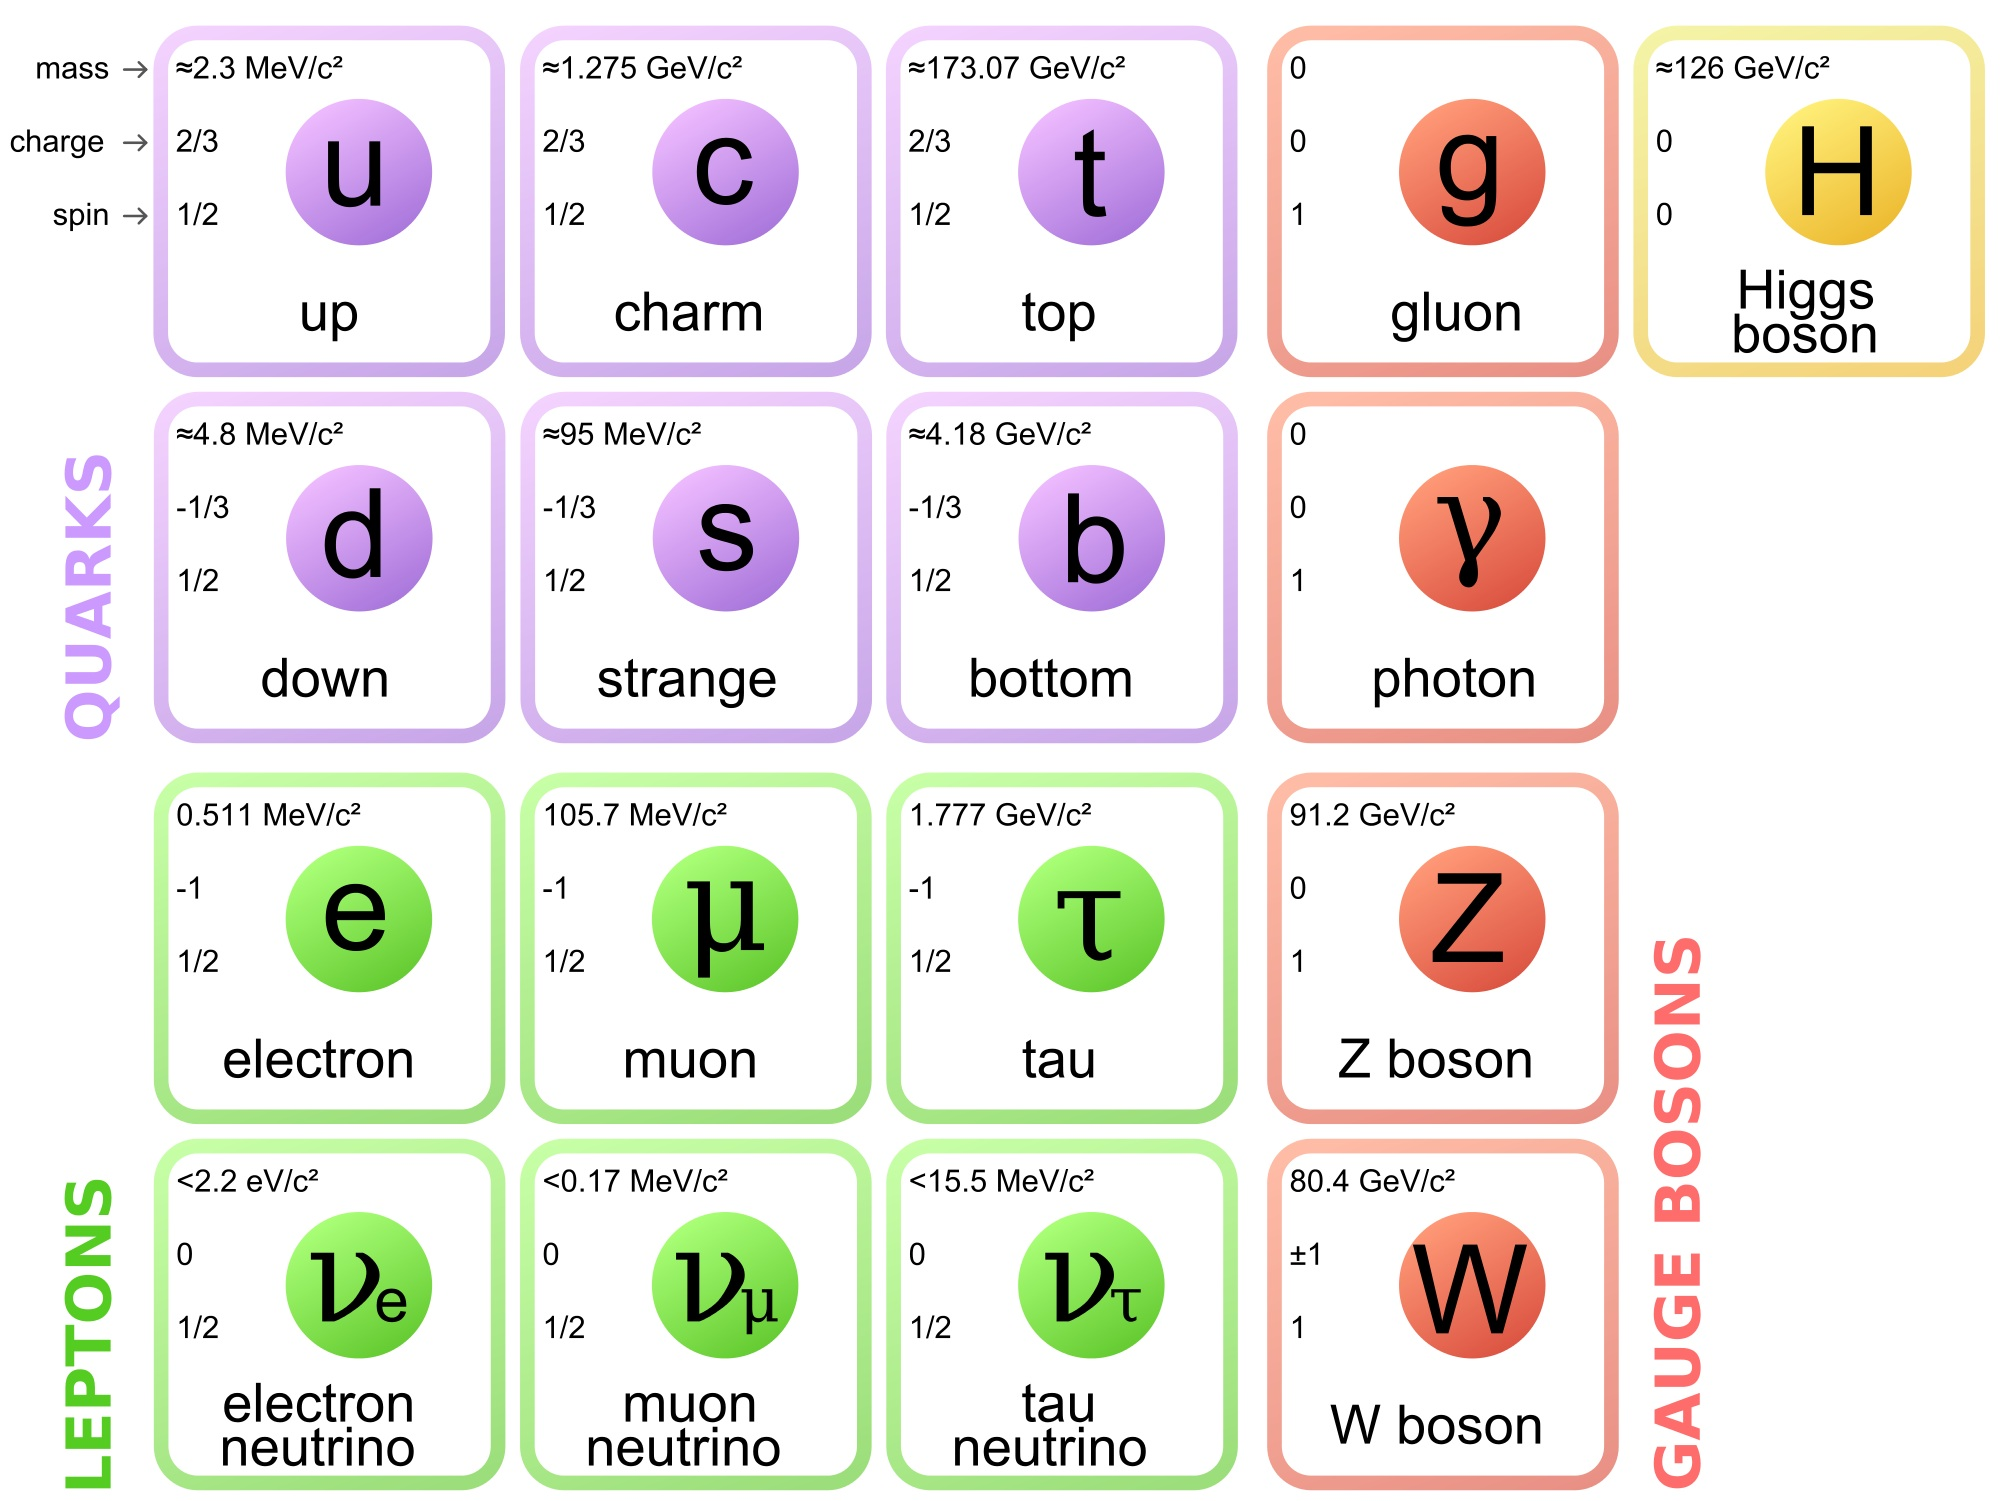
\includegraphics[width = 0.75\textwidth]{Chapter1/SMofElementaryParticles}
%  \caption{Fundamental particles of the Standard Model}
%    \label{fig:Chap1:SM_basic}
%\end{figure}


Before describing the fundamental interactions of the SM in the QFT formalism, it is convenient to introduce 
the two main types of particles according to their spin, i.e. their intrinsic angular momentum: fermions and bosons.

% FERMIONS
\paragraph{Fermions}\mbox{}\\
The fermions are the particles that follow the Fermi--Dirac statistics, i.e. obey the Pauli exclusion principle~\cite{10230794692Dirac}, resulting 
in a distribution of particles over energy levels in which two elements with the same quantum numbers cannot occupy the same states.
The fermions include all particles with half-integer spin: quarks, leptons and baryons.
A baryon is a non-fundamental particle composed of an odd number of valence quarks. 
%\footnote{The hadrons (baryons are mesons) are understood as a sea of partons being the valence quarks those which are more probable to be found in the hadron according to the parton distribution functions.} (consequently having half-integer spin)
%and nearly all matter that
%may be encountered or experienced in everyday life is baryonic matter. Protons and neutrons are examples of baryons.

%Some examples of baryons are\footnote{Between round brackets, the valence quarks are shown.} the proton (\Pup\Pup\Pdown), the 
%neutron (\Pdown\Pdown\Pup), \PLambda (\Pup\Pdown\Pstrange), \PLambdac (\Pup\Pdown\Pcharm) and \PSigmaplus (\Pup\Pup\Pstrange).
%\PDelta (\Pup \Pup \Pdown) The difference between de \PDelta and the proton is the arrangement of the spin of the quarks, 
%Apart from the 3-quark baryons, an exotic pentaquark state has been observed at LHCb experiment of the LHC~\cite{LHCb:2019kea}. 


The fundamental fermionic matter is organised in the three families of leptons 
and quarks, shown also in Table~\ref{tab:Chap1:FundamentalFermions}:

\begin{center}
$\begin{bmatrix}
\Pnue & \Pup \\
\Pelectron & \Pdown 
\end{bmatrix}$
,
$\begin{bmatrix}
\Pnum & \Pcharm \\
\Pmuon & \Pstrange 
\end{bmatrix}$
,
$\begin{bmatrix}
\Pnut & \Ptop \\
\Ptauon & \Pbottom 
\end{bmatrix}$\, .
\end{center}

%where, according to QCD, each quark appears in three different colours:
These three generations, which are defined as the columns in Figure~\ref{fig:Chap1:SM}, exhibit the same kind of 
gauge interactions and they only differ in their mass~\cite{Salam:1968rm}. %~\cite{Pich:2007vu}.
According to the EW symmetry, each family can be classified as:
\begin{center}
$\begin{bmatrix}
\Pnulepton & \ensuremath{\Pquark_{u}} \\
\Pleptonminus & \ensuremath{\Pquark_{d}} 
\end{bmatrix}$
$\equiv$
$\begin{pmatrix}
\Pnulepton \\
\Pleptonminus
\end{pmatrix}_{L}$ ,
$\begin{pmatrix}
\ensuremath{\Pquark_{u}} \\
\ensuremath{\Pquark_{d}} 
\end{pmatrix}_{L}$,
$\Pleptonminus_R$, $\ensuremath{\Pquark_{uR}}$, $\ensuremath{\Pquark_{dR}}$ \, .
\end{center}
(plus the corresponding antiparticles) where the subindices \textit{L} and \textit{R} stand from left- and right-handed particles, respectively. 
This structure responds to the fact that left-handed particles convert differently than right-handed ones under $SU(2)$ transformations.
The left-handed fields are $SU(2)_\text{L}$ doublets and the right-handed ones $SU(2)_\text{L}$ singlets. %This difference is explained with more
%detail in Section~\ref{sec:chap1:EW}. 

%As discussed in the following sections, the weak interaction only affects left-handed particles (and right-handed antiparticles) therefore,
%since the most basic representation of $SU(2)$ is a doublet, the $\begin{pmatrix}
%\Pnulepton \\
%\Pleptonminus
%\end{pmatrix}_{L}$ element appears. The $\Pleptonminus_{R}$ exists because QED affects the charged leptons but not the neutrinos and 
%, since the representation of $U(1)$ is a singlet and this force does not differentiate between eft and right-handed particle, the $\Pleptonminus_{R}$ 
 
%makes no difference between left and right-handed particles and,
%since the charged leptons but not the nautrinos are affected by QED, only the $\Pleptonminus_{R}$ but not the $\Pnulepton_R$ exits.
%The most basic representation of SU(2) is a doublet.
%\pablo{(Why there are right and left charged leptons but only left neutrinos? First of all, because  thy are not observed in Nature 
%and, secondly because the neutrinos are neutral and, hence, its quantum numbers under SM transformations are 1,1,1, i.e. they are singlets)}

The fundamental representation of $SU(3)$ is a triplet, this is why each quark can appear in three different colours, whereas each antiquark can exhibit one of the corresponding ``anticolours''. 

%->. L = Left-polarisation <- Left-handed particles transform different than right handed under SU2 transformations.
%La representación más básica de su2 es un doblete
%y las de su3 son triples (red, green blue)
%Igual que hay lepton right, en el SM no hay neutrino right : In the SM, neutrinos are left handed

%-> Should I introduce the conservation of the leptonic and baryonic numbers?

% Please add the following required packages to your document preamble:
% \usepackage{multirow}

The SM fermions properties are summarised in Table~\ref{tab:Chap1:FundamentalFermions}. 
The neutrino flavour states do not correspond to 
the mass states. What happens is that each 
flavour state is a quantum mechanical combination of neutrinos of different masses and vice versa.
More details about the neutrino masses can be found in a dedicated text in Section~\ref{sec:chap1:SM_problems}.

\begin{table}[]
\centering
\begin{tabular}{lccc}
\toprule
Family                   		& Name              			& Mass [MeV]								& Charge    \\ \midrule
\multirow{6}{*}{Quarks} 	& Up 	 ($\Pup$)                	& $2.16^{+0.49}_{-0.26}$    					& 2/3  \\
                         			& Down     ($\Pdown$)            	& $4.67^{+0.48}_{-0.17}$	 		    			& -1/3  \\
                         			& Charm 	 ($\Pcharm$)            	& (1.27$\pm$0.02)$\times 10^{3}$					& 2/3  \\
                         			& Strange  ($\Pstrange$)          	& $93^{+11}_{-5}$     				& -1/3 \\
                         			& Top  	 ($\Ptop$)              	& $(172.76\pm0.30)\times 10^{3}$     				& 2/3 \\
                         			& Bottom   ($\Pbottom$)          	& $(4.18^{+0.03}_{-0.02})\times 10^{3}$     			& -1/3 \\ \midrule
\multirow{6}{*}{Leptons} 	& Electron  ($\Pelectron$)        	& $0.5109989461\pm0.0000000031$    	& -1   \\
                         			& Muon      ($\Pmu$)		        	& $105.6583745\pm0.0000024$     		& -1   \\
                         			& Tau          ($\Ptau$)     		& $776.86\pm0.12$					& -1   \\
                         			& Electron neutrino ($\Pnue$) 	&	-	& 0\\
                         			& Muon neutrino     ($\Pnum$)	&     	-	 & 0    \\
                         			& Tau neutrino        ($\Pnut$)  	&     	-	 & 0    \\ \bottomrule
\end{tabular}
\caption{Properties of the quarks and leptons. The electric is presented in units 
of elementary charge ($1.602 \times10^{-19}$~C). The neutrino mass eigenstates, which have a fix mass, are 
different from the flavour eigenstates. Therefore, the mass of \Pnue, \Pnum and \Pnut is not defined.}
\label{tab:Chap1:FundamentalFermions}
\end{table}

%The fundamental fermions are usually understood as the fundamental building blocks 
%of matter. However, while the building blocks are important, there is a point that 
%also has to be taken into account, the force. Without force these fermions would 
%not interact which each other. The particles that mediate these interactions are the
%gauge bosons. 


\paragraph{Bosons}\mbox{}\\
Bosons differ from fermions by obeying the Bose--Einstein statistics, thus, bosons are 
not limited to single occupancy for a determined state. In other words, the Pauli exclusion 
principle is not applied. All particles with integer spin are bosons; from the particles shown on the right columns of Figure~\ref{fig:Chap1:SM}
to the mesons. Mesons, along with baryons, are part of the hadron family, i.e. particles composed of quarks (see Section~\ref{sec:chap1:QCD}). 
The particularity of mesons is that they are formed from an equal number of quarks and antiquarks (usually one of each) bound together by strong 
interactions.  Some examples of mesons are $\pi^{\pm , 0}$, $K^{\pm , 0}$ and \PJpsi. %\Ppiplus, \Ppizero, \PKplus and \PJpsi.

%Some examples of mesons are \Ppiplus (\Pup \APdown), \Ppizero ($\frac{\Pup \APup - \Pdown \APdown}{\sqrt{2}}$), \PKplus (\Pup \APstrange) and \PJpsi(\Pcharm \APcharm).
% \Petac (\Pcharm \APcharm) and \PJpsi(\Pcharm \APcharm) have the same quark distribution composition but \Petac is a pseudoscalar and a vector.

The elementary vector bosons are the force carriers and are presented in Table~\ref{tab:Chap1:FundamentalInteractions} while the Higgs boson is a fundamental particle as well. 
%\begin{figure}
%    \centering
%    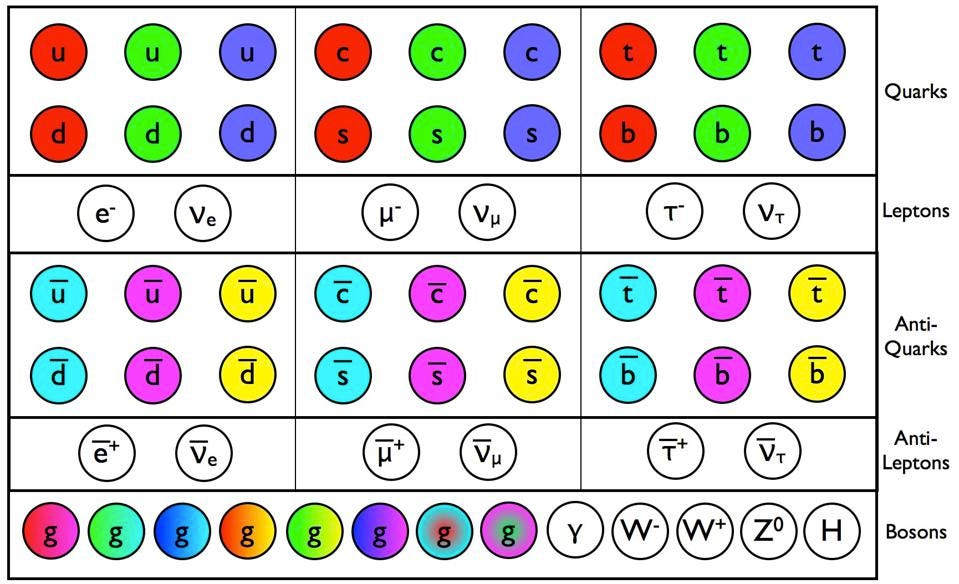
\includegraphics[width = 0.95\textwidth]{Chapter1/SM_Color}
%    \caption{Extended table of the particles composing the SM: Antiparticles and colour charge configurations are included.}
%    \label{fig:Chap1:SM_color}
%\end{figure}


%%%%%%%%%%%%%%%%%%%%%
%              Gauge Invariance                   %
%%%%%%%%%%%%%%%%%%%%%
%\paragraph{Gauge Invariance}\mbox{}\\
%Constituting one of the most successful theories of Physics, the SM is able to provide an elegant mathematical framework to
%describe the experimental physics results with great precision.
%Another key element to understand the SM is the concept of gauge invariance.
%As it is illustrated during the rest of the Section~\ref{sec:chap1:TheSM}, by demanding that 
%the Lagrange density (also denoted as Lagrangian) invariant
%under local gauge transformations, the existence of the SM force-carrier 
%bosons (\Pgamma, \PWplus, \PWminus, \PZ and \Pg). %is predicted through
%the gauge invariant field strength tensors:
%\begin{align*}
%  A  : photon
%  B  : ew
%  W : ew
%  G	 : gluon
%\end{align*}


%%%%%%%%%%%%%%%
%              QED                    %
%%%%%%%%%%%%%%%
% Peskin: http://home.ustc.edu.cn/~gengb/200923/Peskin,%20An%20Introduction%20to%20Quantum%20Field%20Theory.pdf
% notes: http://www.freebookcentre.net/physics-books-download/Relativistic-Quantum-Field-Theory-Lecture-Notes-I.html
\section{Quantum electrodynamics}
\label{sec:chap1:QED}
%The gauge invariance refers to the invariance of a theory under transformations 
%which the theory is said to posses internal symmetry.
%The transformations which are applied in all space-time locations simultaneously 
%are known as ``global'' transformations while the ones that vary from one point to 
%another are ``local''. Each local symmetry is the basis of a gauge theory and requires 
%the introduction of its own gauge bosons as it is discussed in the following pages.

In QFT, particles are described as excitations of quantum fields that satisfy the corresponding mechanical field equations.
The Lagrangians in QFT are used analogous to those of classical mechanics, where the equation of motion can be derived from the Lagrangian density
function ($\mathcal{L}$) and the Euler--Lagrange equations for fields:
\begin{equation*}
\frac{\partial\mathcal{L}}{\partial \phi} - \partial_{\mu} \frac{\partial\mathcal{L}}{\partial (\partial_{\mu} \phi)} = 0 ,
\end{equation*}
where  $\partial_{\mu} = \frac{\partial}{\partial x^{\mu}}$ denotes the partial derivatives with respect to the four-vector $x^{\mu}$ and 
$\phi = \phi(\overrightarrow{x},t)$ is the quantum field of a given fermion or boson. % A continuous quantity with a value at each point in space-time.
The Lagrangian is used to express the dynamics of the quantum field. In QFT, Noether's theorem~\cite{Noether1918}
relates a symmetry in the $\mathcal{L}$ to a conserved current. %Classical physics
%examples of how the symmetries leads to conserved quantities are:
%\begin{itemize}
%	\item Invariance under change of time $\rightarrow$ Conservation of energy
%	\item Invariance under translation in space $\rightarrow$ Conservation of momentum
%	\item Invariance under rotation $\rightarrow$ Conservation of angular momentum
%\end{itemize}

The Dirac equation, $(i \gamma^{\mu}\partial_{\mu} - m)\Psi(x)=0$, is one of the simplest relativistic field equations. Its Lagrangian
describes a free Dirac fermion:

\begin{equation}\label{eq:chap1:Dirac1}
\mathcal{L}_{0} = i \bar{\Psi}(x) \gamma^{\mu} \partial_{\mu} \Psi(x) - m \bar{\Psi}(x) \Psi(x) ,
\end{equation}
being $\Psi$ and $\bar{\Psi}$ the wave function of the particle and its hermitic conjugate, $\gamma^{\mu}$ 
are the Dirac matrices and $m$ the rest-mass of the fermion.
% In the limit m->0 Dirac equation reduces to the Weyl equation
%The gamma matrices build a set of orthogonal basis vectors for covariant vectors in a Minkowski space.
The first term of $\mathcal{L}_{0}$ is the kinetic term while the second is the mass term. 

%This Lagrangian is invariant under $U(1)$ global transformations such as:
%\begin{equation}\label{eq:chap1:DiracGlobalTransformation}
%\Psi(x) \xrightarrow{\text{U(1)}} \Psi'(x) \equiv exp\{ i Q \theta \} \Psi(x),
%\end{equation}
%where $Q \theta$ is a real constant. The phase of $\Psi(x)$ is a pure convention-dependent quantity without a physical meaning since  the observables depend on $|\Psi(x)|^{2}$.


%However, if $\theta$ was $x$ dependent, the transformation \ref{eq:chap1:DiracGlobalTransformation} would be:
%\begin{equation}\label{eq:chap1:qedLocalTransf}
%\Psi(x) \xrightarrow{\text{U(1)}} \Psi'(x) \equiv exp\{ i Q \theta (x) \} \Psi(x),
%\end{equation}
%which is not longer a global transformation but a local
%transformation instead. The transformation in \ref{eq:chap1:qedLocalTransf} would not let the $\mathcal{L}_{0}$ in \ref{eq:chap1:Dirac1} 
%invariant because the derivative in the kinetic term would go as:
%\begin{equation}\label{eq:chap1:derivativeTransformation}
%\partial_{\mu}\Psi(x) \xrightarrow{\text{U(1)}} exp\{ i Q \theta \} (\partial_{\mu} + iQ\partial_{\mu}\theta)\Psi(x).
%\end{equation}

%The gauge principle is the requirement that the $U(1)$ phase invariance should hold locally.
%In order to do so, it is necessary to introduce an additional term to the Lagrangian so that when one applies $\Psi'(x) \equiv exp\{ i Q \theta (x) \} \Psi(x)$, 
%the $\partial_{\mu}\theta$ term is canceled in \ref{eq:chap1:derivativeTransformation}.
%To achieve this invariance, a term with the vector gauge field $A_{\mu}$ is inserted. This field transforms as
%\begin{equation}\label{eq:chap1:AmuTransformation}
%A_{\mu}(x) \xrightarrow{\text{U(1)}} A_{\mu}'(x) \equiv A_{\mu}(x)+\frac{1}{e}\partial_{\mu}\theta
%\end{equation}
%with a new $D_{\mu}$, which acts as follows:  %covariant derivative:
%\begin{equation}\label{eq:chap1:NewQEDderivative}
%D_{\mu} \Psi(x) \equiv [ \partial_{\mu} + ieQA_{\mu}(x)]\Psi(x)
%\end{equation}
%which transforms like the field:
%\begin{equation*}\label{eq:chap1:QED_DerivativeTransformation}
%D_{\mu} \Psi(x) \xrightarrow{\text{U(1)}} (D_{\mu} \Psi)'(x) \equiv  exp\{ i Q \theta \} D_{\mu}\Psi(x).
%\end{equation*}

The gauge principle requires that the $U(1)$ phase invariance should hold locally. To satisfy
this, the Lagrangian density for quantum electrodynamics (QED) can be defined by replacing the partial derivatives in $\mathcal{L}_{0}$ (equation~\ref{eq:chap1:Dirac1}) with the covariant derivatives: %in \ref{eq:chap1:NewQEDderivative}:
\begin{equation}\label{eq:chap1:Dirac2}
\begin{split}
	\mathcal{L}_{\text{QED}} &\equiv i \bar{\Psi}(x) \gamma^{\mu} D{\mu} \Psi(x) - m \bar{\Psi}(x) \Psi(x) \\
				&=  i \bar{\Psi}(x) \gamma^{\mu} [ \partial_{\mu} + ieQA_{\mu}(x)] \Psi(x) - m \bar{\Psi}(x) \Psi(x) \\
				%&=  i \bar{\Psi}(x) \gamma^{\mu} \partial_{\mu} \Psi(x) -\bar{\Psi}(x) \gamma^{\mu}eQA_{\mu}\Psi(x)   - m \bar{\Psi}(x) \Psi(x) \\
				&= \mathcal{L}_{0} - eQA_{\mu}\bar{\Psi}(x)\gamma^{\mu}\Psi(x).
\end{split}
\end{equation}

The covariant derivative $D_{\mu}= \partial_{\mu} + ieQA_{\mu}(x)$ is defined this way to ensure gauge invariance. 
Here, $A_{\mu}$ is a gauge vector field that transforms like this:
 $A_{\mu}(x) \xrightarrow{\text{U(1)}} A_{\mu}'(x) \equiv A_{\mu}(x)+\frac{1}{e}\partial_{\mu}\theta$ 

Therefore, the Lagrangian in equation~\ref{eq:chap1:Dirac2} is invariant under $U(1)$ local transformation. 
%When the conversions \ref{eq:chap1:qedLocalTransf} and 
%\ref{eq:chap1:AmuTransformation} take place, the effects of the transformation are canceled out. 
Along with the original Lagrangian in equation~\ref{eq:chap1:Dirac1}, the $\mathcal{L}_{\text{QED}}$ has an additional term describing the interaction 
between the fermion $\Psi$ and the gauge field $A_{\mu}$ with a strength proportional to the charge $eQ$. 
This term, $eQA_{\mu}\bar{\Psi}\gamma^{\mu}\Psi$, which has been generated only by demanding the gauge invariance
under $U(1)$, is not other than the vertex of QED. %(Figure~\ref{fig:Chap1:QED_Vertex}). 
%\begin{figure}
%    \centering
%    \includegraphics[width = 0.35\textwidth]{Chapter1/QED_vertex}
 %   \caption{Three-point interaction vertex of QED.}
 %   \label{fig:Chap1:QED_Vertex}
%\end{figure}

This new $A_{\mu}$ term is the electromagnetic field and its quanta is the photon.
A mass term containing $A^{\mu}A_{\mu}$ is forbidden because it would violate the $U(1)$ local invariance. 
Consequently, the mediator of the new $A_{\mu}$ field, the photon, is predicted to be a massless particle. 
To make $A_{\mu}$ a propagating field it is necessary to add the kinetic term of the field $A_{\mu}$:
\begin{equation}\label{eq:chap1:QED_Kin}
	\mathcal{L}_{\text{kin}} \equiv - \frac{1}{4}F_{\mu \nu}(x) F^{\mu \nu}(x),
\end{equation}
where $F_{\mu \nu} \equiv \partial_{\mu} A_{\nu} -\partial_{\nu} A_{\mu}$. 
The kinetic term  $F_{\mu \nu} F^{\mu \nu}$ is already invariant under local $U(1)$ phase transformations.
%From the QED Lagrangian in \ref{eq:chap1:Dirac2} and the kinetic term in \ref{eq:chap1:QED_Kin},
%the Maxwell equations can be derived to describe electromagnetism, the infinite range\footnote{Since the photon is (predicted to be) massless, the electromagnetic interaction has an infinite range.} 
%interaction that occurs between particles with electrical charge.
The $\mathcal{L}_{\text{QED}}$  with this kinetic term is written as:
\begin{equation}\label{eq:chap1:QED_Complete}
	\mathcal{L}_{\text{QED}} =  \bar{\Psi}(x) (i  \gamma^{\mu} \partial_{\mu} - m ) \Psi(x) - eQ \bar{\Psi}(x) \gamma^{\mu}A_{\mu} \Psi(x) - \frac{1}{4}F_{\mu \nu}(x) F^{\mu \nu}(x).
\end{equation}


%%%%%%%%%%%%%%%
%          ElectroWeak            %
%%%%%%%%%%%%%%%
\section{Electroweak interaction}
\label{sec:chap1:EW}

\subsubsection{Weak interactions and symmetries}
The weak interaction is mediated by the $W^{\pm}$ and $\PZ$ massive gauge bosons. 
%$\PWplus$, $\PWminus$ and $\PZ$ massive gauge bosons.
The range of the interactions is within a scale of $\sim 10^{-18}$ m. %($m_{\PWpm} =  80.4$ GeV and $m_{\PZ} =  91.2$ GeV)
It is responsible for radioactive decays and flavour-changing\footnote{The lepton charge (also called lepton number) is conserved for every leptonic family.} decays of fermions such as the decay of 
the muon ($\Pmuon \rightarrow \Pelectron \APneutrino_{e} \Pneutrino_{\mu}$).


Another particularity of this interaction is that it is the only interaction that violates several fundamental symmetries. 
The three discrete symmetries that are fundamental for the SM formulation and always hold for the
electromagnetic and strong interactions but not for the weak interactions are:
\begin{itemize}
	\item \textbf{Charge conjugation (C)}: Replace positive quantum charges by negative charges and vice versa. %This symmetry is behind
										%the conservation of lepton number, baryon number and strangeness.
										It does not affect mass, energy, momentum or spin. Essentially, it is a 
										transformation that switches
										all particles with their corresponding antiparticles.
										%\begin{align*}
											%\mathcal{C} \ket{ \Psi} = \ket{\bar{\Psi}}
											%\mathcal{C} \Psi(\overrightarrow{r}, t) = \bar{\Psi}(\overrightarrow{r}, t)
										%\end{align*}
										 
	\item \textbf{Parity (P)}: Parity involves a transformation that changes the algebraic sign of the spatial coordinate system. 
								%It transforms a phenomenon by inverting its spatial coordinates through the origin. 
								It does not reverse time, mass, energy or other scalar quantities.
								%\begin{align*}
									%\mathcal{P}:\begin{pmatrix} x \\ y \\ z \end{pmatrix} \rightarrow \begin{pmatrix} -x \\ -y \\ -z \end{pmatrix} &&
									%\hat{\mathcal{P}} \Psi(r) = e^{i \frac{\theta}{2}} \Psi(-r)
									%\mathcal{P} \Psi(\overrightarrow{r}, t) = \Psi(-\overrightarrow{r}, t)
								%\end{align*}
	\item \textbf{Time reversal (T)}: Consists in flipping the sign of the time.
								%\begin{align*}
									%\mathcal{T}:t \rightarrow -t &&
									%\mathcal{T} \Psi (\overrightarrow{r}, t) = \Psi (\overrightarrow{r}, -t)
									%\mathcal{T} \Psi(t, \overrightarrow{x})\mathcal{T}^{-1} = \Psi(-t, \overrightarrow{x})
 								%\end{align*}
\end{itemize}

%\paragraph{\CP-symmetry}\mbox{}\\
The simultaneous combination of these three symmetries mentioned above results in the CPT symmetry, a profound symmetry of QFT which is
consistent through all experimental observations~\cite{Streater:1989vi}. If CPT symmetry is conserved, particles and their respective antiparticles 
are predicted to have, for example, the same mass and lifetime. %The SM is structured on the pillars of CPT symmetry and Lorentz invariance.
Meanwhile, the P and C symmetries can be combined to create the \CP symmetry, the product of the two transformations.
The weak interaction violates P and C symmetries and the combined \CP symmetry. 
Therefore, through the CPT theorem~\cite{Bell:1955djs}, if the \CP is violated,
T is violated as well to preserve the CPT invariance~\cite{Streater:1989vi}. %This has been verified experimentally
 The \CP violation plays a fundamental role in explaining the dominance of 
 matter over antimatter in the present universe. 
% Direct \CP violation is allowed in the SM if a complex phase is present in the CKM matrix.
The ``direct'' \CP violation is a phenomenon where the same decay process has a different probability for a 
particle than for an antiparticle. The measurement of the \tHq cross-section %\footnote{The cross-section concept is 
%introduced in Section~\ref{sec:Chap1:LHC:Cross-Section}.} 
allows us to determine the possible existence of a \CP-violating 
phase as it is further discussed in Section~\ref{sec:Chap1:tHq}.


%\paragraph{Parity and Charge conjugation violation}\mbox{}\\
%\paragraph{Parity violation}\mbox{}\\
%Previously theorised by Lee and Yang~\cite{Lee:1956qn}, the confirmation of the non-conservation of $\mathcal{P}$ in weak interactions 
%arrived with the Wu experiment in 1957~\cite{Wu:1957my}. %A more detailed overview of \CP violation is developed in Section~\ref{sec:chap1:CP_Violation}.
%Studying the beta decay of the Cobalt-60, Wu and collaborators found that the neutrino 
%and the antineutrino have the relative orientations of spin and linear momentum fixed.
%The neutrino spin is always opposite to the linear momentum, this is called left-handed particles.
%Meanwhile, for the antineutrinos, the momentum is always aligned in the same direction as the spin (right-handed particles).
%This causes the weak interactions which emit neutrinos or antineutrinos to violate the conservation of parity.

%Only left-handed particles and right-handed antiparticles are sensitive to the weak force. Dirac fermion fields, $\psi$, exhibit 
%chiral symmetry and the right and left handed chiral states can be expressed as:
%\begin{align}
%	\psi_{L }(x) &= \frac{1}{2} (1-\gamma_{5})\psi (x) \equiv P_{L}  \psi (x) \\
%	\psi_{R }(x) &= \frac{1}{2} (1+\gamma_{5}) \psi (x) \equiv P_{R}  \psi (x)
%\end{align}
%with
%\begin{align*}
%	\gamma^{5} &\equiv \gamma_{5} \equiv \gamma^{0}\gamma^{1}\gamma^{2}\gamma^{3} = \begin{pmatrix} 1 & 0 \\ 0 & 1 \end{pmatrix}
%\end{align*}
%where $P_{L}$ and $P_{L}$ are known as projection operators. The last equality is valid in the Dirac representation.
%This requires a more complex structure to describe weak interactions.

%In the same year, the $\mathcal{C}$ violation was found too~\cite{PhysRev.105.1415}. \pablo{Describe how the $\mathcal{C}$ violation was discovered}


%CP VIOLATION
%\paragraph{\CP violation}\mbox{}\\
%While $\mathcal{P}$ and $\mathcal{C}$ are violated in a maximal way by the weak interactions, 
%the product of these two discrete transformations, \CP, is still a good symmetry (left-handed fermions 
%$\leftrightarrow$ right-handed fermions).  Experiences such as the Wu experiment respect the \CP 
%symmetry and, in fact, in the \CP is a symmetry of nearly all the observed phenomena. However, in 
%1964 Cronin and Fitch discovered a slight (2\%) violation of the \CP symmetry in the decays of neutral 
%kaons~\cite{Christenson:1964fg}. The \CP violation plays a fundamental role to explain the dominance of
%matter over antimatter in the present universe. More information about the matter--antimatter asymmetry
%can be found in the dedicated text in Section~\ref{sec:chap1:SM_problems}. 

%Direct \CP violation is allowed in the SM if a complex phase is present in the CKM matrix (described below).
%The ``direct'' \CP violation is a phenomenon where the same decay process has a different probability for a 
%particle than for an antiparticle. An example of strong global \CP asymmetry observed corresponds to the decay
%into two kaons and one pion. The probability of $\PBplus \rightarrow \Ppiplus \PKplus \PKminus$ is 20\% higher 
%than for $\PBminus \rightarrow \Ppiminus \PKplus \PKminus$. 

%Source: https://moriond.in2p3.fr/2022/EW/slides/5/1/6_RCardinale-v1.pdf
%source: https://home.cern/news/news/physics/largest-matter-antimatter-asymmetry-observed
%So far, $\mathcal{CPT}$ is the only symmetry that stands unviolated and, given that \CP is not, the $\mathcal{T}$ must be violated as well. %Already commented

%Quizás discutir la relevancia que tiene CP en esta tesis

\paragraph{CKM matrix}\mbox{}\\
The eigenstates that interact through weak interactions, known as ``weak eigenstates'' 
(\Pdown', \Pstrange', \Pup'), are different from the physically observed mass eigenstates 
(\Pdown, \Pstrange , \Pup). This makes possible the charged-flavour-changing-weak decays
through the Cabibbo--Kobayashi--Maskawa (CKM) matrix.
The CKM matrix, $V_{\text{CKM}}$, describes the mixing between the three generations of quarks in the SM. 
The coupling of two quarks $i$ and $j$ to a \PW boson is proportional to the CKM matrix element $V_{ij}$.
\begin{equation*}
	\begin{pmatrix} \Pdown' \\ \Pstrange ' \\ \Pup ' \end{pmatrix}  = \begin{pmatrix} 	V_{ud} & V_{us} & V_{ub} \\
																V_{cd} & V_{cs} & V_{cb} \\ 
																V_{td}  & V_{ts}  & V_{tb} \end{pmatrix}
												 \begin{pmatrix} \Pdown \\ \Pstrange  \\ \Pup  \end{pmatrix}
\end{equation*}

It is a $3 \times 3$ unitary matrix described by four independent parameters: three angles and one complex phase. 
These angles are known as the Euler angles and the phase allows the \CP violation~\cite{Chau:1984fp}. 
The largest values correspond 
to the diagonal elements of the matrix.
This implies that the processes that do not change the flavour are strongly preferred over the 
family-changing charged currents. 

%Different equivalent representations of the CKM matrix can be found in literature but the Particle Data Group recommends the standard CKM
%parameterisation:

%\begin{equation}
%V_{CKM} = 	\begin{pmatrix}	
%						c_{12}c_{13}				&                  -s_{12} c_{13}					& s_{13}e^{-i \delta_{13}} 	\\
%			-s_{12}c_{23}-c_{12}s_{23}s_{13}e^{i\delta_{13}}	& -c_{12}c_{23}-s_{12}s_{23}s_{13}e^{i\delta_{13}}	& s_{23}c_{13} 			\\
%			s_{12}s_{23}-c_{12}c_{23}s_{13}e^{e\delta_{13}}	& -c_{12}s_{23}-s_{12}c_{23}s_{13}e^{i\delta_{13}}	& c_{23}c_{13}
%			\end{pmatrix}		
%\end{equation}
%where $c_{ij} \equiv \textrm{cos}\,\theta_{ij}$ and  $s_{ij} \equiv \textrm{sin}\,\theta_{ij}$, 
%with $i$ and $j$ labelling the generations ($i,\,j \in \{1,2,3\}$).
%The angles $\theta_{12}$,  $\theta_{23}$ and  $\theta_{13}$ are known as Euler angles.  
%The complex phase $\delta_{13}$ allows the \CP violation~\cite{Chau:1984fp}.
%There are other popular parameterisations such as the Kobayashi-Maskawa one
%or the Wolfenstein one. 

%The different elements of the CKM matrix are determined experimentally and are
%summarised in Table~\ref{tab:Chap1:CKM}.
 %As can be seen in this table,  the largest values correspond to the diagonal elements of the CKM matrix.
%This implies that the processes that do not change the flavour are strongly preferred over the 
%family-changing charged currents. For instance, for the top quark, the decay to any of the three down-type 
%quarks is allowed but only $|V_{td}|^{2}\times 100\% = 0.0064\%$ of times will decay to a down quark and
% $|V_{ts}|^{2}\times 100\% = 0.14\%$ to a strange quark.
%(using lowest value of $V_{tb} within its uncertainty) $|V_{tb}|^{2} \times 100 = 97 $

%\begin{table}[]
%\centering
%\begin{tabular}{c|l l}
%\begin{tabular}{c|l }
%\toprule
%CKM element 	  & Value \\
%\midrule
%   $V_{ud}$         &   $0.9740 \pm 0.00011$	%& 	\cite{Hardy:2017G0}~\cite{Pocanic:2003pf}  									
%   	\\
%   $V_{us}$         &   $0.22650 \pm 0.00048$    	%&	\cite{PhysRevLett.41.1692}~\cite{Cabibbo:2003ea}  								
%   	\\
%   $V_{cd}$         &   $0.22636 \pm 0.0048$    		%&	\cite{FlavourLatticeAveragingGroup:2019iem}~\cite{BaBar:2014xzf}~\cite{CLEO:2009svp} 	
%   	\\
%   $V_{cs}$         &   $0.97340\pm0.011$		%&	\cite{CHORUS:2005nog}\cite{BaBar:2010ixw} ~\cite{Belle:2006idb} 					
%   	\\
%   $V_{cb}$         &   $0.04053^{+0.00083}_{-0.00061}$	    	%&	\cite{HFLAV:2019otj}\cite{Belle:2017rcc}										
%   	\\
%   $V_{ub}$         &   $0.00361^{+0.00011}_{-0.00009}$   	%&	\cite{BaBar:2011xxm}~\cite{Colquhoun:2015mfa}\cite{Bauer:2000xf}\\ %\cite{Neubert:1993um}
%  	\\ 	
%   $V_{td}$          &   $0.00854^{+0.00023}_{-0.00016}$    	%&	\cite{LHCb:2013lrq}\cite{Misiak:2015xwa}										
%   	\\
%   $V_{ts}$          &   $0.03978^{+0.00082}_{-0.00060}$  		%&	\cite{LHCb:2013lrq}\cite{Misiak:2015xwa}										
%   	\\
%   $V_{tb}$          &   $ 0.999172^{+0.000024}_{-0.000035}$ 		%&	\cite{CDF:2015gsg}\cite{CMS:2015nrd}\cite{D0:2011viq}		
%   	\\
%\bottomrule
%\end{tabular}
%\caption{Magnitude of the nine elements of the CKM matrix. The mean for the different measurements has been done by~\cite{ParticleDataGroup:2020ssz}. Note how the elements that refer to quarks of the same generation are favoured over the flavour-changing currents.}
%\pablo{Igual me he venido arriba con las referencias. Son las que daba el Particle Data Group}
%\label{tab:Chap1:CKM}
%\end{table} %source: https://pdg.lbl.gov/2021/reviews/contents_sports.html


% is currently believed that CP-violation during the early universe can account for the "excess" matter, although the debate is not settled
%The \CP violation reflects the asymmetry between matter and antimatter. \pablo{ \CP violation was found with kaon oscillations <- Cite this discovery}

%La violacion cp se debe a que hay tres familias -> la fase compleja de la matriz CKM es la única fuente de violación cp


 %CPviolation depends on the CKM matrix elements associated with weak phase and strong phase:
% page 8: https://arxiv.org/pdf/2201.02385.pdf
% CP violation in ckm matrix: https://arxiv.org/pdf/hep-ph/0406184.pdf page 7

%Due to its ability to change the flavour of quarks and leptons, the theory describing the behaviour of the weak force is the quantum flavourdynamics but
%this term is rarely used because this interaction is better understood by the EW theory.
 
%\pablo{check:~\cite{Hung:2021tmi}}


\subsection{Electroweak unification}
%After the discovery of $\mathcal{P}$ in Wu experiment, a search began to relate weak and electromagnetic interactions.
%Glashow-Salam-Weinberg model
At energies above the scale of the mass of the weak vector bosons ($E_{\text{EW}} \sim m_{Z} \sim m_{W} \sim 100\,\textrm{GeV}$), the electromagnetic 
and weak interactions are unified into the electroweak (EW) force. In other words, electromagnetism and weak interactions are simultaneously described by the symmetry group $SU(2)_{\text{L}} \bigotimes U(1)_\text{Y}$. 
The subindex $\text{L}$ refers to left-handed fields and $\text{Y}$ to the weak hypercharge, a quantum number conserved under the strong interaction.  In contrast, at low energies, these interactions are treated as independent phenomena, 
the electromagnetism is described by the QED and the weak interaction proposed by E.~Fermi.

In the EW model (i.e. Glashow--Salam--Weinberg model), two new quantum numbers  are assigned to the particles of the SM: the weak isospin ($\overrightarrow{T}$) and weak hypercharge $\text{Y}'$.
Here, the left-handed chiral states of fermions form isospin doublets ($\chi_\text{L}$) with $\text{T}_{3} = \pm 1/2$ and the right-handed form chiral states are composed of isospin singlets ($\chi_\text{R}$)  with $\text{T}_{3} = 0$.
For a particle, $\text{T}_{3}$ is the third component of the $\overrightarrow{\text{T}}$, which is related to the electric charge ($Q$) and the $U(1)$ weak hypercharge by Gell-Mann--Nishijima relation:
\begin{equation}\label{eq:chap1:EW:GMN}
	Q = \text{T}_{3} + \frac{1}{2} \text{Y}' \, .
\end{equation}
%where the hypercharge is defined defined by the strangeness, charmnes, etc etc as
%https://physics.stackexchange.com/questions/379888/are-both-gell-mann-nishijima-formulas-true-for-the-same-reason
%
Through this expression, the electromagnetic coupling and the electroweak couplings are connected.
Having $\chi_\text{L}$ with $\text{T}_{3} = \pm 1/2$ and $\chi_\text{R}$  with $\text{T}_{3} = 0$ implies that a $SU(2)$ weak interaction can rotate left-handed particles 
(i.e. convert a left-handed \Pelectron into a left-handed $\Pneutrino_{e}$ emitting a \PWminus) but cannot do the same with right-handed.

Using the gauge invariance principle it is possible to find the QED Lagrangian: %and QCD Lagrangians, 
%as it is respectively described in Sections \ref{sec:chap1:QED} and \ref{sec:chap1:QCD}.
%The free Lagrangian, as in the case of QED and QCD is:
\begin{equation}\label{eq:chap1:EW:LagrangianFree}
\begin{split}
	\mathcal{L} 	&= i \sum_{j=1}^{3} \bar{\Psi}(x) \gamma^{\mu} \partial_{\mu} \Psi(x) \\
				& = i \sum_{j=1}^{3} \bar{\chi_\text{L}}(x) \gamma^{\mu} \partial_{\mu} \chi_\text{L}(x)+  i \sum_{k=1}^{3} \bar{\chi_\text{R}}(x) \gamma^{\mu} \partial_{\mu} \chi_\text{R}(x)
\end{split}
\end{equation}
where the wave function $\Psi$ has been split into the left isospin doublets $\chi_\text{L}$ and right isospin singlets $\chi_\text{R}$. 
The indices $j$ and $k$ run over 
the three generations of the SM. 
%This Lagrangian should be invariant when a gauge transformation under the $SU(2)_{L} \times U(1)_{Y}$ symmetry group in the flavour space is applied:
%\begin{align}
%	\chi_\text{L}(x) 	&\xrightarrow{\text{$SU(2)_{L} \times U(1)_{Y}$}} \chi_\text{L}'(x) =  exp\{ i \alpha^{n} \tau_{n} \}\, exp\{ i \beta y \}\,\chi_\text{L}(x) \\
%	\chi_\text{R}(x) 	&\xrightarrow{\text{$SU(2)_{L} \times U(1)_{Y}$}} \chi_\text{R}'(x) =  exp\{ i \beta y \} \,\chi_\text{R}(x)
%\end{align}
%with $\alpha, \, \beta \in \mathds{R}$ and $n \in \{1,2,3 \}$.
%This transformation is given by the generators of $SU(2)_{L} \times U(1)_{Y}$, i.e. the Pauli matrices ($\tau_{n}$) and the weak hypercharge $y$. 
%Note that $SU(2)_L$ transformation, $exp\{ i \alpha^{n} \tau_{nu} \}$, only acts on the doublet fields. This term containing the Pauli matrices is 
%non-abelian like in QCD and, like in QCD, this leads to self-interacting terms.

%To ensure invariance under  $SU(2)_{L} \times U(1)_{Y}$, four different gauge fields have to be added (three from $SU(2)$ and one from $U(1)$).
%Four is also the correct number of gauge bosons needed to describe EW interactions: \PWplus, \PWminus, \PZ and \Pgamma.
%While the three week isospin currents couple to the triplet of vector bosons $\PW^{n}_{\mu}$ with $n \in \{1,2,3 \}$, the weak hypercharge
%couples to an isosinglet $B_\mu$.  The fields $\PW^{1}_{\mu}$ and $\PW^{2}_{\mu}$ are electrically charged whereas $\PW^{3}_{\mu}$ and $B_\mu$
%are neutral fields. 
%The EW covariant derivative is defined as:
%\begin{align}
%	D^{\mu} \chi_{\text{L}_{j}}(x)	& =  [\partial_{\mu} - i g \frac{\tau_{i}}{2}\PW^{i}_{\mu}(x)  - i g' \frac{y_j}{2}  B_{\mu}(x) ] \, \chi_{\text{L}_{j}} (x)  &&  i \in [1,2,3] 	\label{eq:chap1:EW:CovariantDerivatice1} \\
%	D^{\mu} \chi_{\text{R}_{j}}(x)	& = [\partial_{\mu} - i g' \frac{y_j}{2}  B_{\mu}(x)] \,\chi_{\text{R}_{j}}(x)		,										\label{eq:chap1:EW:CovariantDerivatice2}
%\end{align}
%where $g$ and $g'$ are the interaction couplings to $\PW^{i}_\mu$ isotriplet and the $B_{\mu}$ isosinglet.

%Using the derivatives in equation~\ref{eq:chap1:EW:CovariantDerivatice1} and \ref{eq:chap1:EW:CovariantDerivatice2}, the Lagrangian 
%in \ref{eq:chap1:EW:LagrangianInvariant} is already invariant under local $SU(2)_{L} \times U(1)_{Y}$ transformations:
%\begin{equation}\label{eq:chap1:EW:LagrangianInvariant}
%	\mathcal{L} = i \sum_{j=1}^{3} \bar{\chi_\text{L}}^{j}(x) \gamma^{\mu} D_{\mu} \chi_\text{L}^{j}(x)+  i \sum_{k=1}^{3} \bar{\chi_\text{R}}^{k}(x) \gamma^{\mu} D_{\mu} \chi_\text{R}^{k}(x) 
%\end{equation}

To ensure gauge invariance under  $SU(2)_{\text{L}} \times U(1)_{\text{Y}}$, four different gauge 
fields have to be added. % (three from $SU(2)$ and one from $U(1)$)
While three week-isospin currents couple to the triplet of vector bosons $\PW^{n}_{\mu}$ 
with $n \in \{1,2,3 \}$, the weak hypercharge couples to an isosinglet $B_\mu$.
The fields $\PW^{1}_{\mu}$ and $\PW^{2}_{\mu}$ are electrically charged 
whereas $\PW^{3}_{\mu}$ and $B_\mu$ are neutral fields. 
The EW covariant derivative is defined as:
\begin{align}
	D^{\mu} \chi_{\text{L}_{j}}(x)	& =  [\partial_{\mu} - i g \frac{\tau_{i}}{2}\PW^{i}_{\mu}(x)  - i g' \frac{y_j}{2}  B_{\mu}(x) ] \, \chi_{\text{L}_{j}} (x)  &&  i \in [1,2,3] 	\label{eq:chap1:EW:CovariantDerivatice1} \\
	D^{\mu} \chi_{\text{R}_{j}}(x)	& = [\partial_{\mu} - i g' \frac{y_j}{2}  B_{\mu}(x)] \,\chi_{\text{R}_{j}}(x)		,										\label{eq:chap1:EW:CovariantDerivatice2}
\end{align}
where $g$ and $g'$ are the interaction couplings to $\PW^{i}_\mu$ isotriplet and the $B_{\mu}$ isosinglet.
Finally, if kinetic terms for the gauge bosons are included, the EW SM Lagrangian is obtained:
\begin{equation}
\begin{split}\label{eq:chap1:EW:FinalL}
	\mathcal{L}_{\text{EW}}  =	& i \sum_{j=1}^{3} \bar{\chi_\text{L}}^{j}(x) \gamma^{\mu} D_{\mu} \chi_\text{L}^{j}(x)+  i \sum_{k=1}^{3} \bar{\chi_\text{R}}^{k}(x) \gamma^{\mu} D_{\mu} \chi_\text{R}^{k}(x) \\
					& - \frac{1}{4} W^{n}_{\mu \nu}(x)W_{n}^{\mu \nu}(x) - \frac{1}{4} B_{\mu \nu}(x)B^{\mu \nu}(x) \, ,
\end{split}
\end{equation}
where the addition of kinetic terms gives rise to cubic and quadratic self-interactions among the gauge fields.
%Note that the mass terms of the fields are forbidden to ensure local gauge invariance.
%Since the observed $\PWplus$, $\PWminus$ and $\PZ$ bosons have masses different from zero, 
%it is necessary to assume that something breaks the symmetry generating the observed masses.
%In Section~\ref{sec:chap1:ParticleMasses}, the symmetry breaking is explained.

%This Lagrangian describes the interactions between gauge vector bosons and fermions below
%\begin{align*}
%	\chi_\text{L} 	&& =  \begin{pmatrix} \Pnue \\ \Pe  \end{pmatrix}_{L} & \begin{pmatrix} \Pnum \\ \Pmu  \end{pmatrix}_{L} & \begin{pmatrix} \Pnut \\ \Ptau  \end{pmatrix}_{L} & \begin{pmatrix} \Pup \\ \Pdown  \end{pmatrix}_{L} &\begin{pmatrix} \Pcharm \\ \Pstrange  \end{pmatrix}_{L} &\begin{pmatrix} \Ptop \\ \Pbottom \end{pmatrix}_{L}   \\
%	\chi_\text{R} 	&&=	 \Pe_{R} & \Pmu_{R} & \Ptau_{R} & \Pup_{R}  \Pdown_{R} & \Pcharm_{R}  \Pstrange_{R} & \Ptop_{R}   \Pbottom_{R}
%\end{align*}
%\pablo{Esto se ve muy feo: Editar $\chi_\text{L}$ y $\chi_\text{L}$.}

The $\mathcal{L}_{\text{EW}}$ in equation~\ref{eq:chap1:EW:FinalL} can be divided in two different parts according 
to the charge of the bosons: charged currents and neutral currents.
Relating the charged currents ($\PW^{1}_{\mu}$ and $\PW^{2}_{\mu}$) to the \PWplus and \PWminus 
bosons of the SM and the neutral ($\PW^{3}_{\mu}$ and $B_\mu$) ones with the $\PZ$ and $\Pgamma$, 
it is possible to build linear combinations of the original gauge fields that define the SM bosons.

%\pablo{Reescribir a partir de aquí para que quede más bonito\\}

%Therefore, from the charged-current interactions, the $\PWplus$ and $\PWminus$ bosons 
%are:
%\begin{equation}
%	\PWpm \equiv \frac{1}{\sqrt{2}}(\PW^{1}_{\mu} \mp i\PW^{2}_{\mu})\, .
%\end{equation}

%While for the neutral-current these combinations can be defined as a rotation of the so called Weinberg 
%(or weak mixing) angle $\theta_{W}$:
%\begin{equation*}\label{eq:chap1:EW:ZmuAmu}
%		\begin{pmatrix} \PW_{\mu}^3 \\ B_\mu \end{pmatrix} \equiv
%		\begin{pmatrix} \textrm{cos} \,\theta_{W} & \textrm{sin} \,\theta_{W} \\  -\textrm{sin} \,\theta_{W} & \textrm{cos}\, \theta_{W} \end{pmatrix} \begin{pmatrix} \PZ_{\mu} \\ A_{\mu} \end{pmatrix} \, .
%\end{equation*}
%Rewriting this equation, the photon and $\PZ$-boson fields are 
%\begin{align}
%	A_{\mu}	&= B_{\mu} \textrm{cos} \,\theta_{W}+ W^{3}_{\mu}  \textrm{sin} \,\theta_{W}
%	Z_{\mu}	&= -B_{\mu} \textrm{cos} \,\theta_{W}+ W^{3}_{\mu}  \textrm{sin} \,\theta_{W} \, .
%\end{align}
%In order to ensure that this $A_{\mu}$ is the one of QED, apart from the Gell-Mann-Nishijima relation (Eq.
%\ref{eq:chap1:EW:GMN}), it is required that the couplings of the \Pgamma, \PWpm and \PZ satisfy the relation:
%\begin{equation}
%	g \, \textrm{sin} \,\theta_{W} = g' \,\textrm{cos}\, \theta_{W} = e \, .
%\end{equation}

%Within the unified EW  model, once $ \theta_{W}$ is known, the mass of $\PZ$ is specified.
%Current measurements of $ \theta_{W}$ give a value of $\textrm{sin}^{2} \theta_{W} = 0.2310 \pm 0.0005$~\cite{CMS:2018ktx}. 

%\pablo{Comentar algo el GIM mechanism y las FCNC }


There is no mass term for the bosons in the EW Lagrangian that has been obtained in 
equation~\ref{eq:chap1:EW:FinalL} by demanding the $SU(2)_{L} \times U(1)_\text{Y}$ local invariance, 
which enters in contradiction with the experimental observations for the \PW and \PZ 
bosons that indicate that $m_{Z,W}$ is $\mathcal{O}(100)$~GeV.  
The introduction of such a mass term would break the symmetry, however,  
it is possible to add the mass for the \PW and \PZ bosons without losing the properties of the symmetry. 
The method to do so is known as the Englert--Brout--Higgs mechanism
or, more commonly, just the Higgs mechanism. This mechanism is described in Section~\ref{sec:chap1:ParticleMasses}.


%SU(2) con U(1) te da los bosons de W.Z y fotón pero sin masa 
%También  dan las corrientes que se observan experimentalmente

%Tomas $SU(2) \times U(1)$ y lo rompes a través del SSB, salen los W, Z y fotón con las masas que tocan  
%Romper la simetría pero conservando la local gauge invariance. 

%Al incluir el campo de Higgs, el Lagrangiano obtenido es invariante (es invariante en escalas energéticas de EW, es decir, $m_H$ hacia arriba. 
%y por debajo de esas energías, el lagrangiano ya no es invariante ) bajo $SU(2) \times U(1)$ pero los ``estados de la teoría'' no son invariantes 
% porque el estado vacío de la teoría no permanece invariante y, por lo tanto, el resto de estados tampoco. %Lo que se hace aquí es pasa al gauge unitario,



% From EW to Higgs https://cds.cern.ch/record/475776/files/9811456.pdf

%%%%%%%%%%%%%%%
%              QCD                    %
%%%%%%%%%%%%%%%
\section{Quantum chromodynamics}
\label{sec:chap1:QCD}
The QCD theory is a QFT-based model for describing the strong interactions between 
quarks and gluons (partons). This type of interaction is responsible of 
the nuclear force, the one that acts between the protons and neutrons of atoms 
binding them together. %Without the strong force, the protons inside the nucleus 
%would push each other apart due to the electromagnetic repulsion. It also holds 
%the quarks within a hadron together. 

%%%%%%
% Quarks and Colour
%%%%%%%
\subsection{Quarks and colour}%\mbox{}\\

The QCD theory is based on the $SU(3)$ symmetry group and its name derives from the ``colour'' charge, an analogous to the electric charge of QED but for strong interactions.
The colour charge was introduced in 1964~\cite{Greenberg:1964pe} to explain how quarks could coexist within some hadrons apparently having the same 
quantum state without violating the Pauli exclusion principle. To satisfy the Fermi--Dirac statistics it is necessary to add an additional quantum number, the
colour, to the theory. Each specie of quark ($q$) may have three different colours ($q^{\alpha}$, $\alpha=$1, 2, 3): red, green, and blue.
Baryons and mesons are described then by colour singlet combinations.%:
%\begin{align*}
%B = \frac{1}{\sqrt{6}} \epsilon^{\alpha \beta \gamma} \ket{\Pquark_{\alpha}\Pquark_{\beta}\Pquark_{\gamma}} &&  M= \frac{1}{\sqrt{3}} \epsilon^{\alpha \beta} \ket{\Pquark_{\alpha}\APquark_{\beta}} \, .
%\end{align*} 

Additionally, it is postulated that all hadrons must have a global neutral colour charge, i.e. the hadrons must be ``colourless''. This assumption is known as  the
confinement hypothesis and it is made to avoid the existence of non-observed extra states with non-zero colour. It is called colour confinement because it implies
that it is not possible to observe free quarks since they carry colour charge and, hence, they have to be confined within colour-singlet combinations.
% Figure~\ref{fig:Chap1:ColourCharge}  depicts how different colours and anticolours combine to create the ``colourless'' state.

%\begin{figure}
%\centering
%\begin{subfigure}{.5\textwidth}
%  \centering
%  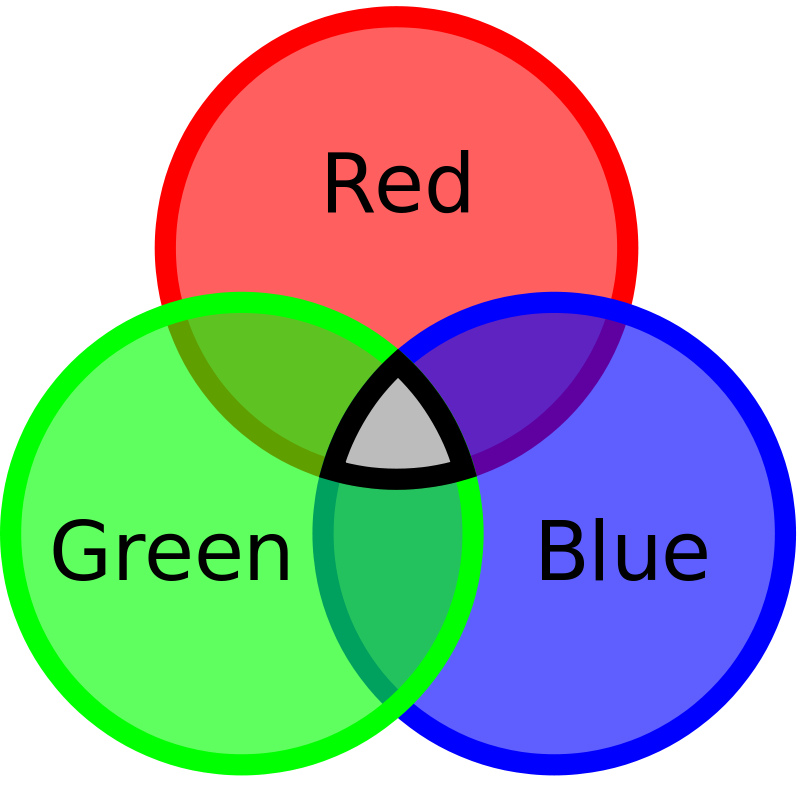
\includegraphics[width=.4\linewidth]{Chapter1/QCD-Colours.png}
%  \caption{Quark colours combine to be colourless.}
%\end{subfigure}%
%\begin{subfigure}{.5\textwidth}
%  \centering
%  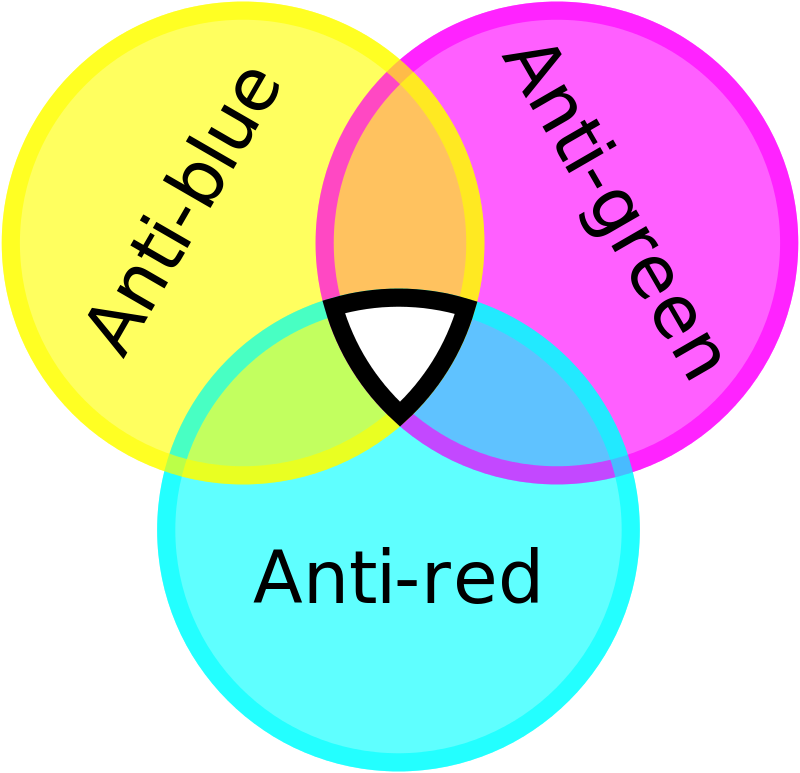
\includegraphics[width=.4\linewidth]{Chapter1/QCD-AntiColours.png}
%  \caption{Antiquark colours also combine to be colourless.}
%\end{subfigure}
%\caption{Colour charge combinations for quarks and antiquarks. Due to the confinement, the hadrons are colourless.}
%\label{fig:Chap1:ColourCharge}
%\end{figure}


%%%%%%
% % Non-Abelian gauge symmetry
%%%%%%%
% https://fse.studenttheses.ub.rug.nl/12978/1/ThesisCasperDijkstra.pdf
\subsection{Gauge invariance for \textit{SU(3)}}%\mbox{}\\
The dynamics of the quarks and gluons are controlled by the QCD Lagrangian. %Using the gauge invariance principle 
%it is possible to deduce $\mathcal{L}_{\text{QCD}}$ similarly to the reasoning developed in Section~\ref{sec:chap1:QED}.
The starting Lagrangian density is
\begin{equation}\label{eq:chap1:QCD:Lagrangian_0}
\mathcal{L}_{0} = \sum_{f} \APquark_{f}^{\alpha} (i \gamma^{\mu} \partial_{\mu} - m_{f})\Pquark_{f}^{\alpha}\, ,
\end{equation}
where $q^{\alpha}_{f}$ denotes a quark field of colour $\alpha$ and flavour $f$. The mass
of $q^{\alpha}_{f}$ is $m_f$. 

The Lagrangian in equation~\ref{eq:chap1:QCD:Lagrangian_0} has to
satisfy invariance under local transformations and hence its derivatives have to be 
substituted by covariant objects. The $SU(N)$ with $N=3$ algebra demands that there are
eight independent gauge parameters and, hence eight different gauge
bosons $G_{a}^{\mu}(x)$ are needed. With $g_{s}$ being the QCD coupling, the
covariant derivatives are:
\begin{equation*}
	D^{\mu}q_{f}^{\alpha} \equiv \big[ \partial_{\mu}  + i g_{s} \frac{\lambda^{a}}{2} G_{a}^{\mu}(x) \big] q_{f}^{\alpha} \equiv [ \partial_{\mu}  + i g_{s} G^{\mu}(x) ] q_{f}^{\alpha} \, .
\end{equation*}
In contrast to the case of QED, the non-commutativity 
of the $SU(3)_\text{C}$ matrices give rise to an additional term involving the gluon 
fields themselves: $- f^{abc}\delta \theta_{b}G_{c}^{\mu}$, with $f^{abc}$ being the
structure constant. With this, it is necessary to introduce the corresponding fields 
strengths to build a gauge-invariant kinetic terms for the gluon fields:
\begin{equation*}
	%G^{\mu \nu}		& \equiv -i\frac{-i}{g_{s}} [D^{\mu}, D^{\nu}] =  \partial_{\mu}G^{\nu} - \partial_{\nu}G^{\mu} + i g_{s}[G^{\mu},G^{\nu}] \equiv \frac{\lambda^{a}}{2}G_{a}^{\mu \nu}(x) \\
	G_{a}^{\mu \nu} \equiv \partial_{\mu}G^{\nu}_{a} - \partial_{\nu}G^{\mu}_{a} - g_{s} f^{abc} G_{b}^{\mu}G_{c}^{\nu}\, .
\end{equation*} 

Normalising the gluon kinetic term, 
the $SU(3)_\text{C}$ invariant QCD Lagrangian is obtained:
\begin{equation}
\label{eq:chap1:QCD:Lagrangian_FinalCompact}
	\mathcal{L}_{\text{QCD}} \equiv  -\frac{1}{4}G^{\mu \nu}_{a} G_{\mu \nu}^{a} + \sum_{f} \APquark_{f}^{\alpha} (i \gamma^{\mu} D_{\mu} - m_{f})\Pquark_{f}^{\alpha} \, .
\end{equation}



%Firstly, let's denote a quark field of colour $\alpha$ and flavour $f$ by $q_{f}^{\alpha}$. 
%The vector $q^{T}_{f}\equiv (q_{f}^{1}, q_{f}^{2}, q_{f}^{3})$ is defined under the $SU(3)$ colour space,  
%meaning that each dimension corresponds to a colour.
%The Lagrangian
%\begin{equation}\label{eq:chap1:QCD:Lagrangian_0}
%\mathcal{L}_{0} = \sum_{f} \APquark_{f} (i \gamma^{\mu} \partial_{\mu} - m_{f})\Pquark_{f}
%\end{equation}
%is invariant under global $SU(3)$ transformation in the colour space,
%\begin{align} \label{eq:chap1:QCD:q_trasnformation}
%q_{f}^{\alpha} \rightarrow (q_{f}^{\alpha})' = U^{\alpha}_{\beta}q^{\beta}_{\alpha}, && UU^{\dagger} = U^{\dagger}U = 1, && \textrm{det }U = 1 .
%\end{align}

%In the $SU(N)$ algebra, $SU(N)$ is the group of $N \times N$ unitary matrices ($U$) which can be written in the form $U = exp \{ i (\lambda^{a}/2) \theta_{a} \}$ with $a = 1,2,...,N^{2}-1$.
%Therefore, the SU(3) matrices can be written as
%\begin{equation}\label{eq:chap1:QCD:U_matrix}
%	U = exp \big\{ i \frac{\lambda^{a}}{2}\theta_{a} \big\}\, ,
%\end{equation}
%where the index $a$ goes from 1 to 8 for the arbitrary parameter $\theta_{a}$ and  $\frac{\lambda^{a}}{2}$, which denotes the fundamental representation of the $SU(3)$ algebra.
%The Einstein notation for summation over repeated indices is implied. The matrices $\lambda^{a}$ are traceless and satisfy the commutation relations~\cite{Pich:2007vu}:
%\pablo{Why does SU(3) has 8 gauge parameters? SU(N) is the group of $N \times N$ unitary matrices ($U$) }%For $SU(N)$  with $N=3$, the fundamental representation correspond to the eight Gell-Mann matrices.2 }
%\begin{equation} \label{eq:chap1:QCD:ConmutationSU3}
%	\big[ \frac{\lambda^{a}}{2}, \frac{\lambda^{b}}{2}\big] = i f^{abc} \frac{\lambda^{c}}{2} \, ,
%\end{equation}
%being $f^{abc}$ the $SU(3)_C$ structure constants, which are real and totally antisymmetric. 

%To satisfy the gauge invariance requirement, the Lagrangian has to be invariant under $SU(3)$ local transformations, i.e, transformations in which 
%the phase is dependent of the space-time location, $\theta_{a} = \theta_{a} (x)$. To fulfil the condition, the quark derivatives in the 
%Lagrangian in \ref{eq:chap1:QCD:Lagrangian_0} have to  be substituted by covariant objets. Since there are eight independent gauge 
%parameters, eight different gauge  bosons $G_{a}^{\mu}(x)$ are needed\footnote{The eightfold multiplicity of gluons is labeled by a combination of   and anti  charge (e.g. red--antigreen)}. 
%This bosons are the eight gluons and  the new covariant objects are:
%\begin{equation*}
%	D^{\mu}q_{f} \equiv \big[ \partial_{\mu}  + i g_{s} \frac{\lambda^{a}}{2} G_{a}^{\mu}(x) \big] q_{f} \equiv [ \partial_{\mu}  + i g_{s} G^{\mu}(x) ] q_{f} \, .
%\end{equation*}
%The compact matrix notation is used  $[G^{\mu}(x)]_{\alpha \beta} \equiv \big( \frac{\lambda^{a}}{2} \big)_{\alpha \beta} G_{a}^{\mu}(x)$.

%To ensure that the covariant derivative ($D^{\mu}q_{f}$) transforms like the $q_f$, the transformation of the gauge fields are:
%\begin{align}\label{eq:chap1:QCD:G_trasnformation}
%	D^{\mu} \rightarrow (D^{\mu})'  = UD^{\mu}U^{\dagger} && G^{\mu} \rightarrow (G^{\mu})' = UG^{\mu}U^{\dagger}+\frac{i}{g_{s}} (\partial_{\mu} U )U^{\dagger} \, .
%\end{align}
%The quark and gluon fields transform under an infinitesimal local transformation, i.e. $\theta_{a} (x) =  \delta \theta_{a}(x) \approx 0$, the $SU(3)_C$ unitary matrices (equation~\ref{eq:chap1:QCD:U_matrix}) can be expressed as their first order expansion:
%\begin{equation*}
%	U = exp \big\{ i \frac{\lambda^{a}}{2}\theta_{a}(x) \big\} \approx 1 + i \big( \frac{\lambda^{a}}{2} \big) \delta \theta_{a}(x)
%\end{equation*}
%and, consequently, the transformations for que colour-vector field (equation~\ref{eq:chap1:QCD:q_trasnformation}) and 
%gluon field (equation~\ref{eq:chap1:QCD:G_trasnformation}) become:
%\cite{Pich:2007vu},
%\begin{align*}
%	q^{\alpha}_{f}	& \rightarrow (q^{\alpha}_{f})' = q^{\alpha}_{f} + \big( \frac{\lambda^{a}}{2} \big)_{\alpha \beta} \delta \theta_{a} q_{f}^{\beta} \\
%	G_{a}^{\mu}	& \rightarrow (G_{a}^{\mu})' =  G_{a}^{\mu} - i \frac{i}{g_{s}} \partial_{\mu} (\delta \theta_{a}) - f^{abc}\delta \theta_{b}G_{c}^{\mu}.
 %\end{align*}
 
%In contrast to the transformation for the photon field in QED (equation~\ref{eq:chap1:AmuTransformation}), 
%the non-commutativity\footnote{Because the generators of $SU(3)$ do not conmute, QCD is known as 
%non-Abelian gauge theory.} of the $SU(3)_C$ matrices give rise to an additional term involving the gluon 
%fields themselves ($- f^{abc}\delta \theta_{b}G_{c}^{\mu}$), as the relation \ref{eq:chap1:QCD:ConmutationSU3} expresses.
%This transformation are more complicated than the ones of equation~\ref{eq:chap1:AmuTransformation}.
%The adjoint representation of an $SU(N)$ group is given by the $(N^{2}-1)\times(N^{2}-1)$ matrices $(\lambda^{a} / 2)_{bc} \equiv -i f^{abc}$.
%For constant $\delta \theta_{a}$, the transformation rule for the gauge fields is expressed in terms of the structure constants $f^{abc}$; 
%thus, the gluon fields belong to the adjoint representation for the colour group. 
%There is a unique coupling at $SU(3)_C$, $g_s$. All the colour-triplet flavours couple to the gluon fields with exactly the same interaction strength. 

%It is necessary to introduce the corresponding fields strengths to build a gauge-invariant kinetic terms for the gluon fields.
%\begin{align*}
%	G^{\mu \nu}		& \equiv -i\frac{-i}{g_{s}} [D^{\mu}, D^{\nu}] =  \partial_{\mu}G^{\nu} - \partial_{\nu}G^{\mu} + i g_{s}[G^{\mu},G^{\nu}] \equiv \frac{\lambda^{a}}{2}G_{a}^{\mu \nu}(x) \\
%	G_{a}^{\mu \nu}	& \equiv \partial_{\mu}G^{\nu}_{a} - \partial_{\nu}G^{\mu}_{a} - g_{s} f^{abc} G_{b}^{\mu}G_{c}^{\nu}\, .
%\end{align*} 

%Under a $SU(3)_C$ transformation,
%\begin{equation}
%	G^{\mu \nu} \rightarrow (G^{\mu \nu})' = UG^{\mu \nu}U^{\dagger}
%\end{equation}
%and the colour trace $\textrm{Tr}(G^{\mu \nu}G_{\mu \nu}) = \frac{1}{2}G^{\mu \nu}G_{\mu \nu}$ remains invariant.  Normalising the gluon kinetic term, 
%the $SU(3)_C$ invariant QCD Lagrangian is obtained:
%\begin{equation}\label{eq:chap1:QCD:Lagrangian_FinalCompact}
%	\mathcal{L}_{\text{QCD}} \equiv   -\frac{1}{4}G^{\mu \nu}_{a}G_{\mu \nu}^{a} + \sum_{f} \APquark_{f} (i \gamma^{\mu} D_{\mu} - m_{f})\Pquark_{f} \, .
%\end{equation}

Note how the gluon--gluon vertex is found by demanding the gauge invariance under local $SU(3)_\text{C}$ transformation.
A mass term is forbidden for the gluon fields by the $SU(3)_\text{C}$  gauge symmetry because a term of the form 
$\frac{1}{2}m^{2}_{G}G^{\mu}_{a}G_{\mu}^{a}$ would not be invariant.
The gluons are, then, predicted by the theory to be spin-1 massless particles.

Thanks to the colour symmetry properties, this Lagrangian looks very simple and all its interactions depend on the strong coupling
constant, $g_s$. In contrast to the Lagrangian derived for QED (see equation~\ref{eq:chap1:Dirac2}), 
in $\mathcal{L}_{\text{QCD}}$ the boson field 
has a self-interacting term. These gluon self-interactions give rise to the triple and quadratic gluon vertex.
The self-interactions among the gluon fields can explain features such as the asymptotic freedom and confinement.
%These properties were not present in QED. 
The asymptotic freedom causes interactions between particles to become asymptotically weaker as the energy 
scale increases and the corresponding length scale decreases. 
The confinement implies that the strong forces increase with the distance, therefore, 
as two colour charges are separated, at some point it becomes energetically favourable 
for a new quark-antiquark pair to appear rather than to keep getting further. These new quarks 
bond with the previous two, preventing single quarks from being isolated. This mechanism, 
depicted in Figure~\ref{fig:Chap1:colorConfinement}, explains graphically why the strong 
interaction is responsible for keeping the quarks together forming hadrons.

%\begin{figure}
%    \centering
%    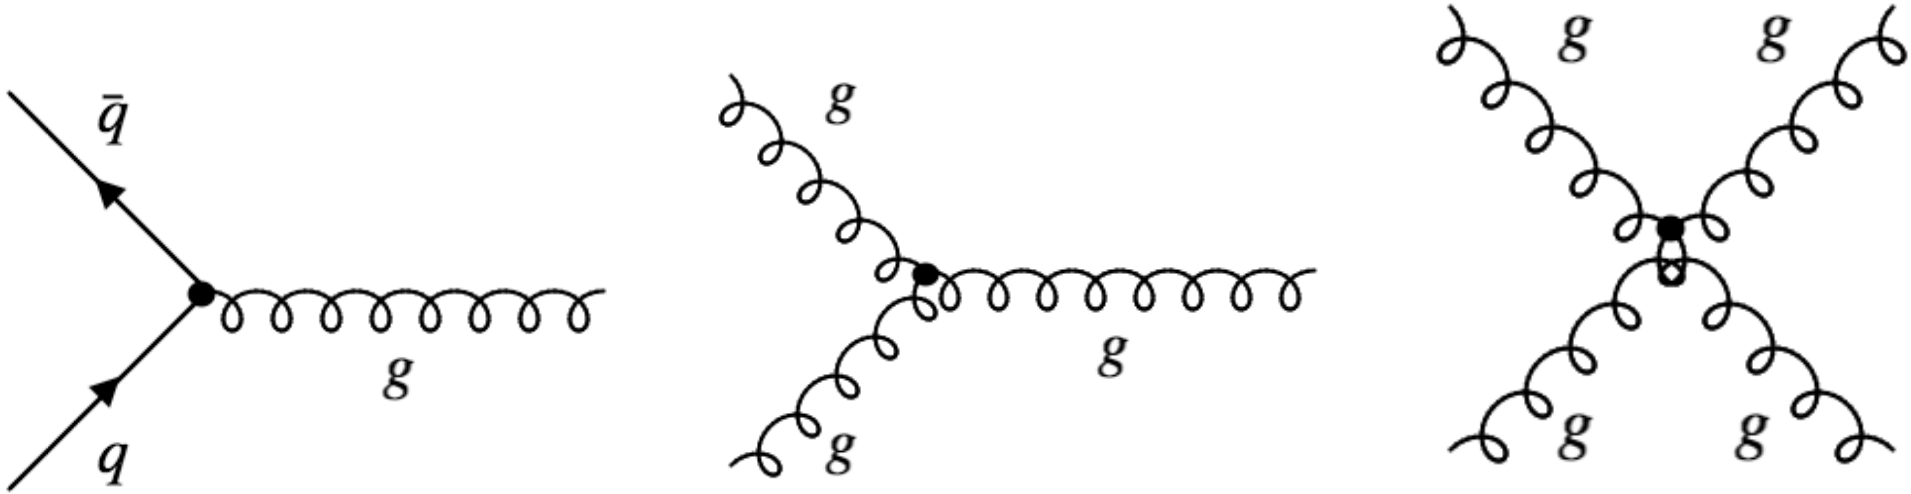
\includegraphics[width = 0.75\textwidth]{Chapter1/QCD_vertex}
%    \caption{The predicted QCD interaction vertices arising from the requirement of $SU(3)_C$ local gauge invariance. The presence of the triples and quadruple gluon vertices is possible to the Non-Abelian nature of $SU(3)_C$.}
%    \label{fig:Chap1:gluonvertex}
%\end{figure}

\begin{figure}[h]
    \centering
    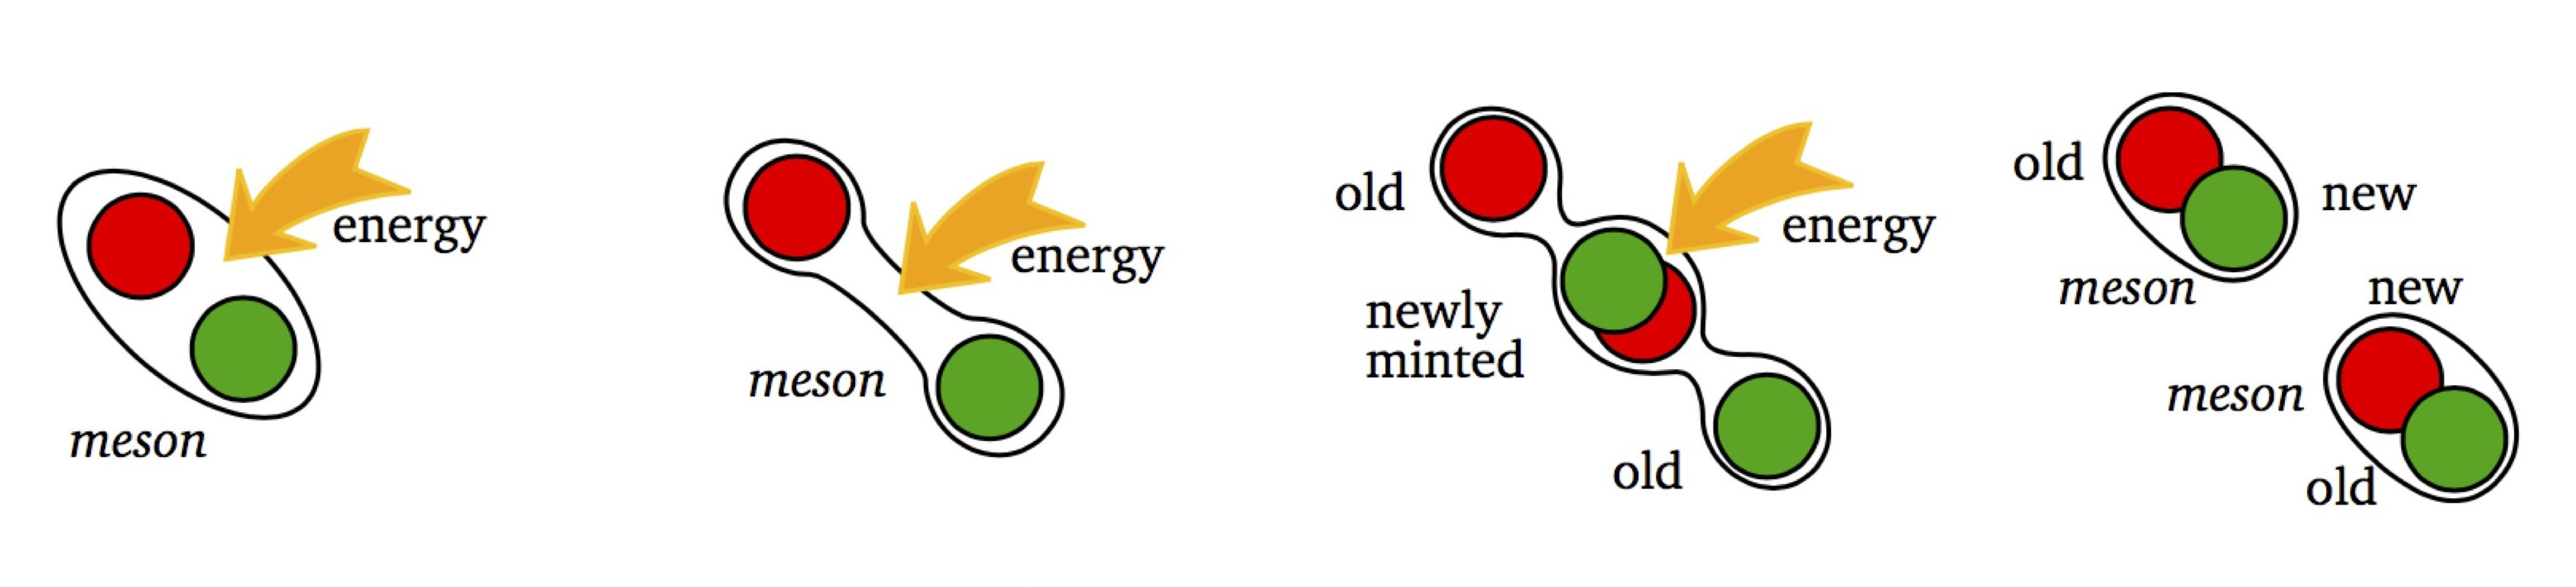
\includegraphics[width = 0.85\textwidth]{Chapter1/ConfinementQCD}
    \caption{The QCD colour confinement explains the inseparability of quarks inside a hadron despite of investing ever more energy. In this example, the mechanism is shown for a meson.}
\label{fig:Chap1:colorConfinement}\end{figure}


%\pablo{Maybe, expand the QCD Lagrangian in \ref{eq:chap1:QCD:Lagrangian_FinalCompact} and explain its different elements.}


%%%%%%%%%%%%%%%%%%%%%
%                  Particle masses                   %
%%%%%%%%%%%%%%%%%%%%%
\section{Particle masses}
\label{sec:chap1:ParticleMasses}
For the QED Lagrangian, $\mathcal{L}_{\text{QED}}$  (see equation~\ref{eq:chap1:QED_Complete}), 
it is clear how the mass of the photon must be zero in order to satisfy the $U(1)$ local gauge symmetry because,
if a mass term for the vector gauge field $A_{\mu}$ is included, the $\mathcal{L}_{\text{QED}}$ would 
be non-invariant.
%if a mass term for the vector gauge field $A_{\mu}$ is included, the $\mathcal{L}_{\text{QED}}$ would be:
%\begin{equation*}\label{eq:chap1:QED_massivephoton}
%	\mathcal{L}_{\text{QED}} =  \bar{\Psi}(x) (i  \gamma^{\mu} \partial_{\mu} - m ) \Psi(x) - eQ \bar{\Psi}(x) \gamma^{\mu}A_{\mu} \Psi(x) - \frac{1}{4}F_{\mu \nu}(x) F^{\mu \nu}(x) + \frac{1}{2}m_{\Pgamma}^{2}A_{\mu}A^{\mu}
%\end{equation*}
%and, with the $U(1)$ transformation in equation~\ref{eq:chap1:AmuTransformation}, the new mass term becomes: 
%\begin{equation*}
%	\frac{1}{2}m_{\Pgamma}^{2}A_{\mu}A^{\mu} \rightarrow \frac{1}{2}m_{\Pgamma}^{2} (A_{\mu} + \frac{1}{e}\partial_{\mu}\theta ) (A^{\mu} +\frac{1}{e}\partial^{\mu}\theta) \neq \frac{1}{2}m_{\Pgamma}^{2}A_{\mu}A^{\mu}\, .
%\end{equation*}
%Confirming that the photon mass term is not invariant under local $U(1)$ and, consequently, that the photon must be massless to satisfy the gauge invariance.
%Experimental efforts to measure the mass of the photon have set an upper limit of $m_{\Pgamma} \leq 1 \times 10^{-18} $ eV~\cite{Ryutov:2007zz}.
%Recent limits form cosmological measurements set the limit in $m_{\Pgamma} \leq 4 \times 10^{-15} $~\cite{Wei:2020wtf}.

The Lagrangian of QCD as presented in equation~\ref{eq:chap1:QCD:Lagrangian_FinalCompact} also demonstrates a similar restriction:
the mass term for the gluon fields is forbidden 
by the $SU(3)_\text{C}$ gauge symmetry. Therefore, the mediating bosons for the strong interactions are massless as well (experimentally, a mass as large as the upper limits
of a few MeV have been set, see Reference~\cite{Yndurain:1995uq}).


While the prohibition of mass terms for the bosons of QED and QCD is not a problem, 
this requirement also applies to the $SU(2)_\text{L}$.
This condition enters into open contradiction with the measurements of large masses for the
%\PW ($m_{\PW} = 80.370 \pm 0.007 \textrm{ (stat.)}\pm 0.017\textrm{ (syst.)}$ GeV~\cite{ATLAS:2017rzl}) 
%and \PZ ($m_{\PZ} = 91.1852 \pm 0.0030$ GeV~\cite{OPAL:2000ufp}) bosons of weak interactions. 
%\pablo{<- to do: Aquí no estoy utilizando las mismas medidas de la masa de $m_{\PW}$ y $m_{\PZ}$ que antes. He %de escoger una and stick to it.}
\PW and \PZ bosons of weak interactions.


For weak interactions, the problem of massless particles does not only affect the bosons. Since under the $SU(2)_\text{L}$ left-handed particles
transform as weak isospin doubles and right-handed particles as isospin singlets, the mass term of a spinor field $\Psi$ written as chiral states also
breaks the required gauge invariance.
% $-m \bar{\Psi}(x) \Psi(x) = -m \bar{\Psi}(x)(P_{R} + P_{L})\Psi(x) = -m (\bar{\Psi}_{R}(x) \Psi_{L}(x) + \bar{\Psi}_{L}(x) \Psi_{R}(x))$

The Englert--Brout--Higgs mechanism~\cite{PhysRevLett.13.321, PhysRevLett.13.508, PhysRevLett.13.585} describes how both the \PW and \PZ bosons and the fermions acquire mass without breaking the local gauge symmetry of the SM. 


%%%%%%%%%%%%%%%%%%%%%
%                  The Higgs mechanism           %
%%%%%%%%%%%%%%%%%%%%%
\subsection{The Englert--Brout--Higgs mechanism}\label{sec:chap1:ParticleMasses:HiggsMechanism}

%\paragraph{Goldstone theorem and spontaneous symmetry breaking}\mbox{}\\
%For a scalar field $\phi$ with a Lagrangian of the form:
%\begin{equation}\label{eq:chap1:HiggsMechanism:Example}
%	\mathcal{L} = \frac{1}{2}\partial_{\mu}\phi_{i}\partial^{\mu}\phi_{i} -V(\phi) \textrm{ where } V(\phi) = \frac{1}{2}\mu^{2}\phi_{i} \phi_{i} + \frac{1}{4}\lambda(\phi_{i} \phi_{i})^{2} \, .
%\end{equation}
%This Lagrangian is invariant under $\phi_{i} \rightarrow \phi_{i}'= R_{ij}\phi_{j}$, where $R_{ij}$ are rotational matrices in 4-dimensions.
% The mass term is the one with $\phi_{i} \phi_{i}$ and 
%the parameter $\lambda$ has to be positive for $\mathcal{L}$ to describe a physical system, if $\lambda$ <0 the potential is unbounded from below.
%Contrary, the parameter $\mu^{2}$ can be either positive or negative. 
%As depicted in Figure~\ref{fig:Chap1:SM:HiggsMechanism:PotentialExample:Positive}, if $\mu^{2}>0$, the vacuum expectation value 
%(i.e. minimum of potential) is located at the origin $\phi_0$ and this $\mathcal{L}$ would describe a spin-0 particle of mass $\mu$. 
%However, if $\mu^{2}<0$, the potential $V(\phi)$ has the form of Figure~\ref{fig:Chap1:SM:HiggsMechanism:PotentialExample:Positive} and $\mathcal{L}$
%would not represent anymore the Lagrangian of a particle of mass $\mu$. The vacuum expectation value is now multivalued:
%\begin{equation*}
%	\phi_{0} = \pm \sqrt{-\frac{\mu^{2}}{\lambda}} \equiv \pm v \, .
%\end{equation*}
%
%\begin{figure}
%\centering
%\begin{subfigure}{.5\textwidth}
% \centering
%  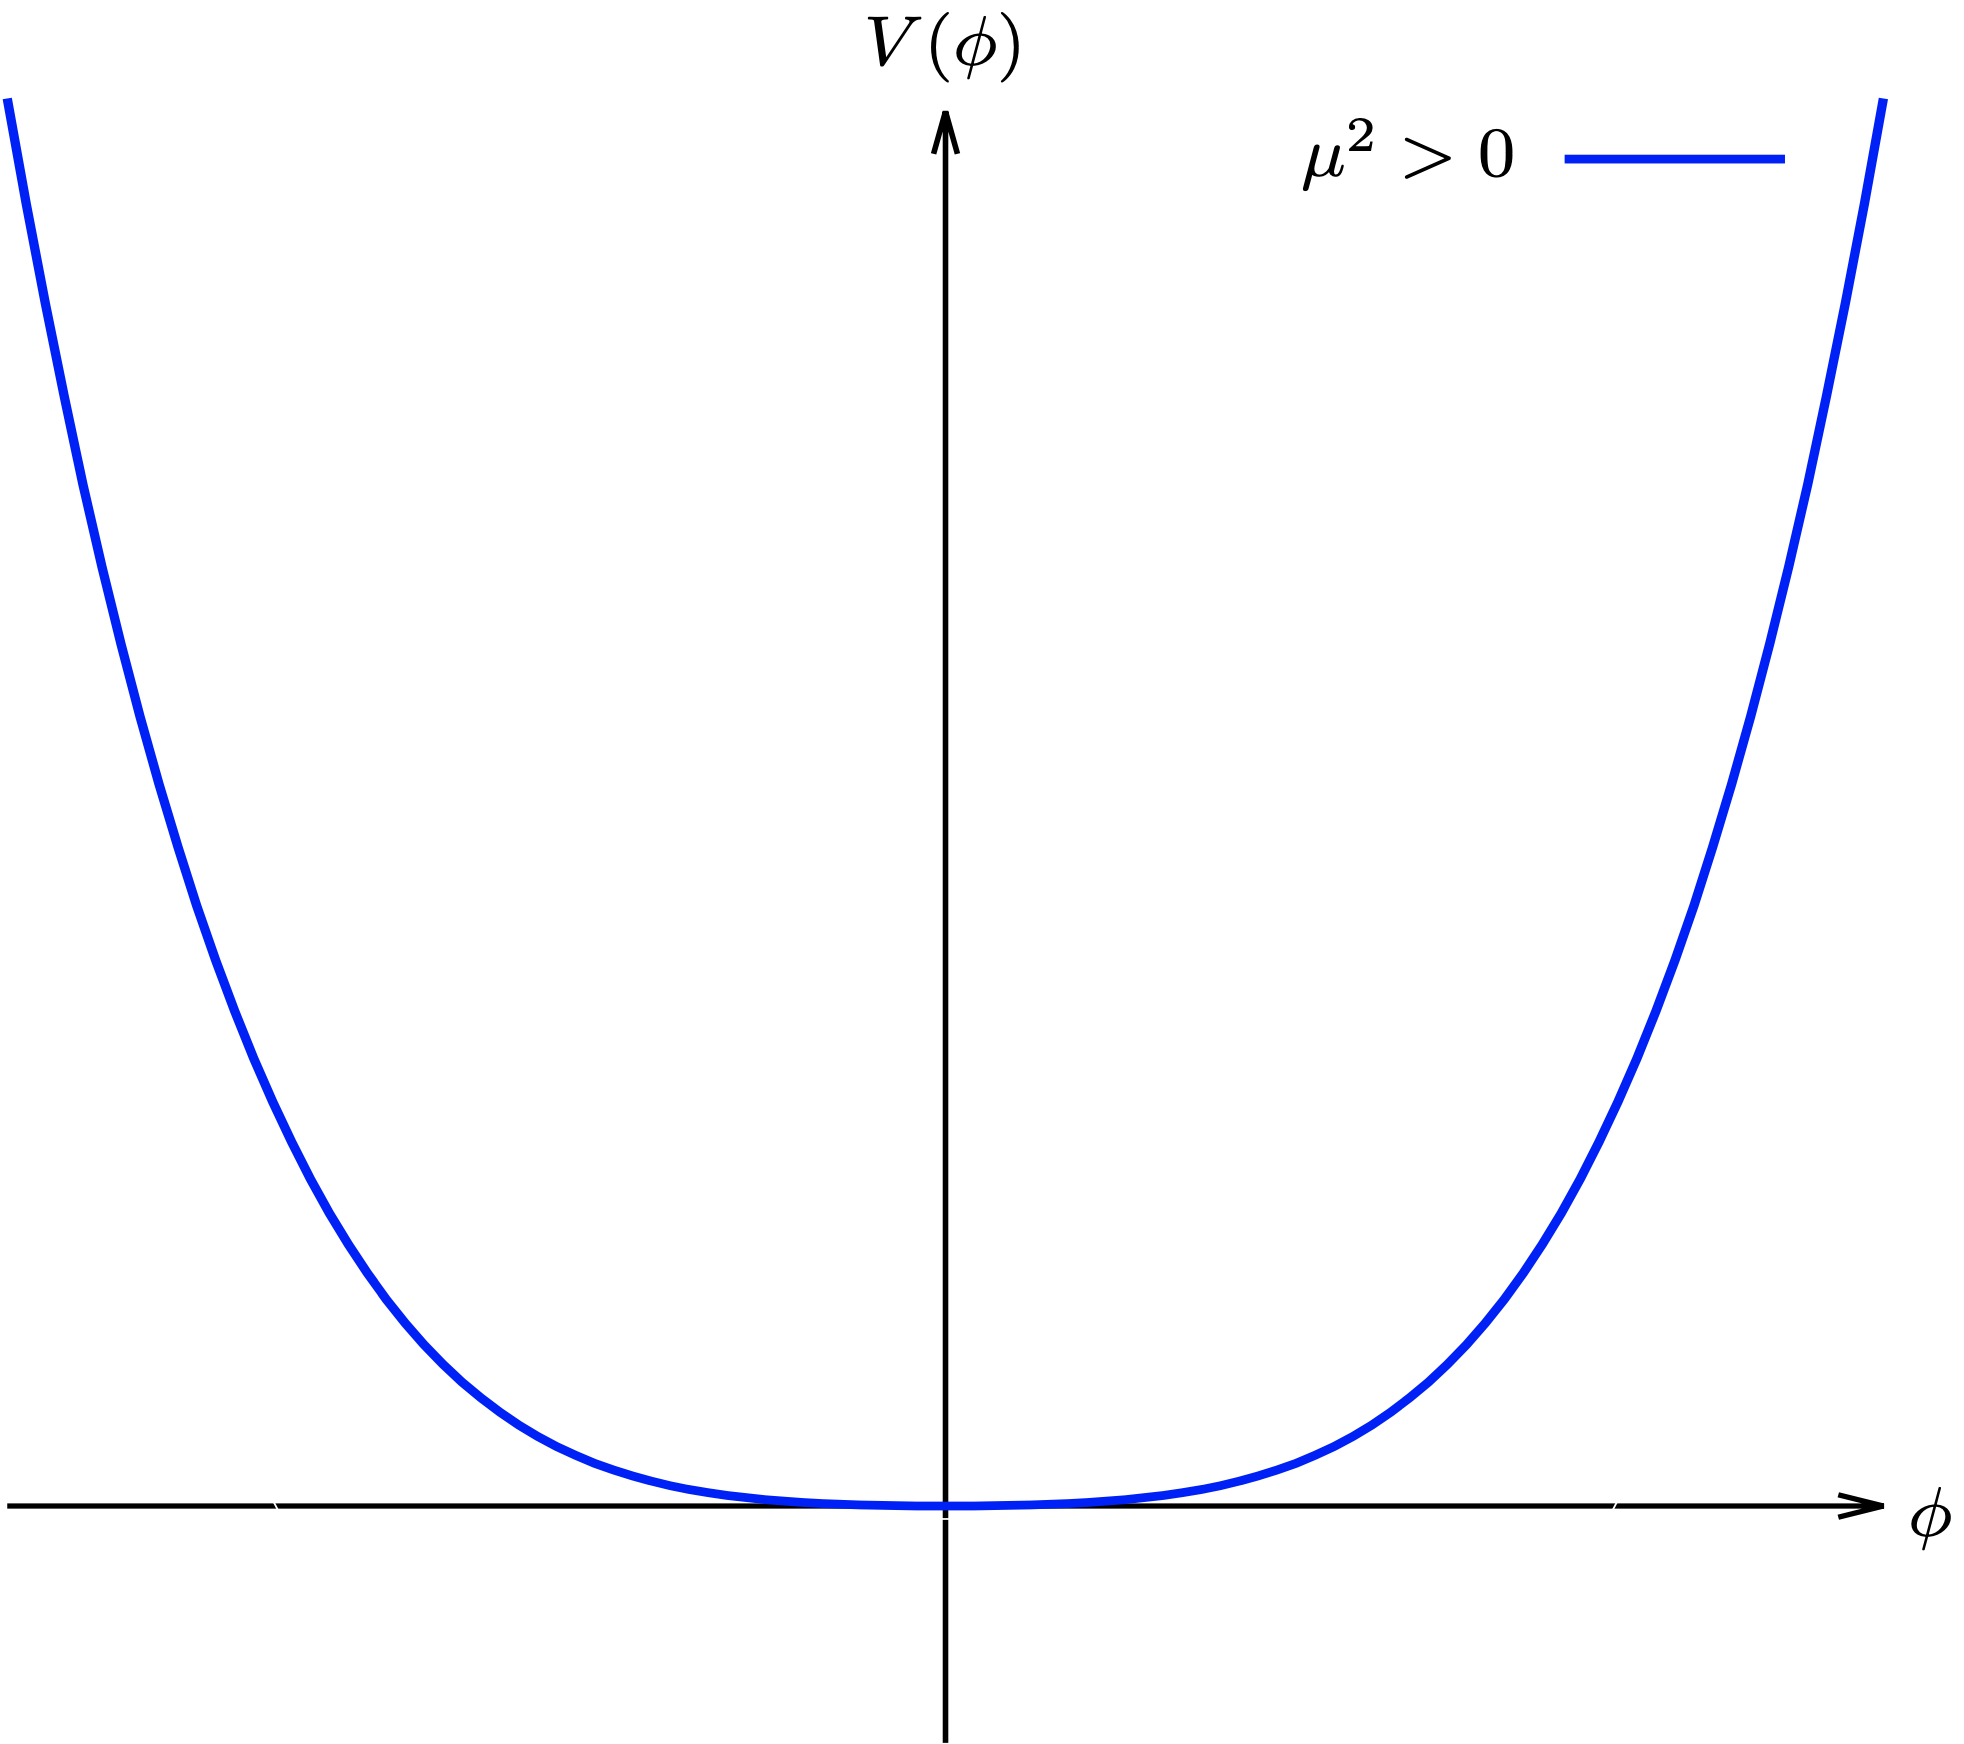
\includegraphics[width=.74\linewidth]{Chapter1/Higgs_V_muplus}
%  \caption{}
%  \label{fig:Chap1:SM:HiggsMechanism:PotentialExample:Positive}
%\end{subfigure}%
%\begin{subfigure}{.5\textwidth}
%  \centering
%  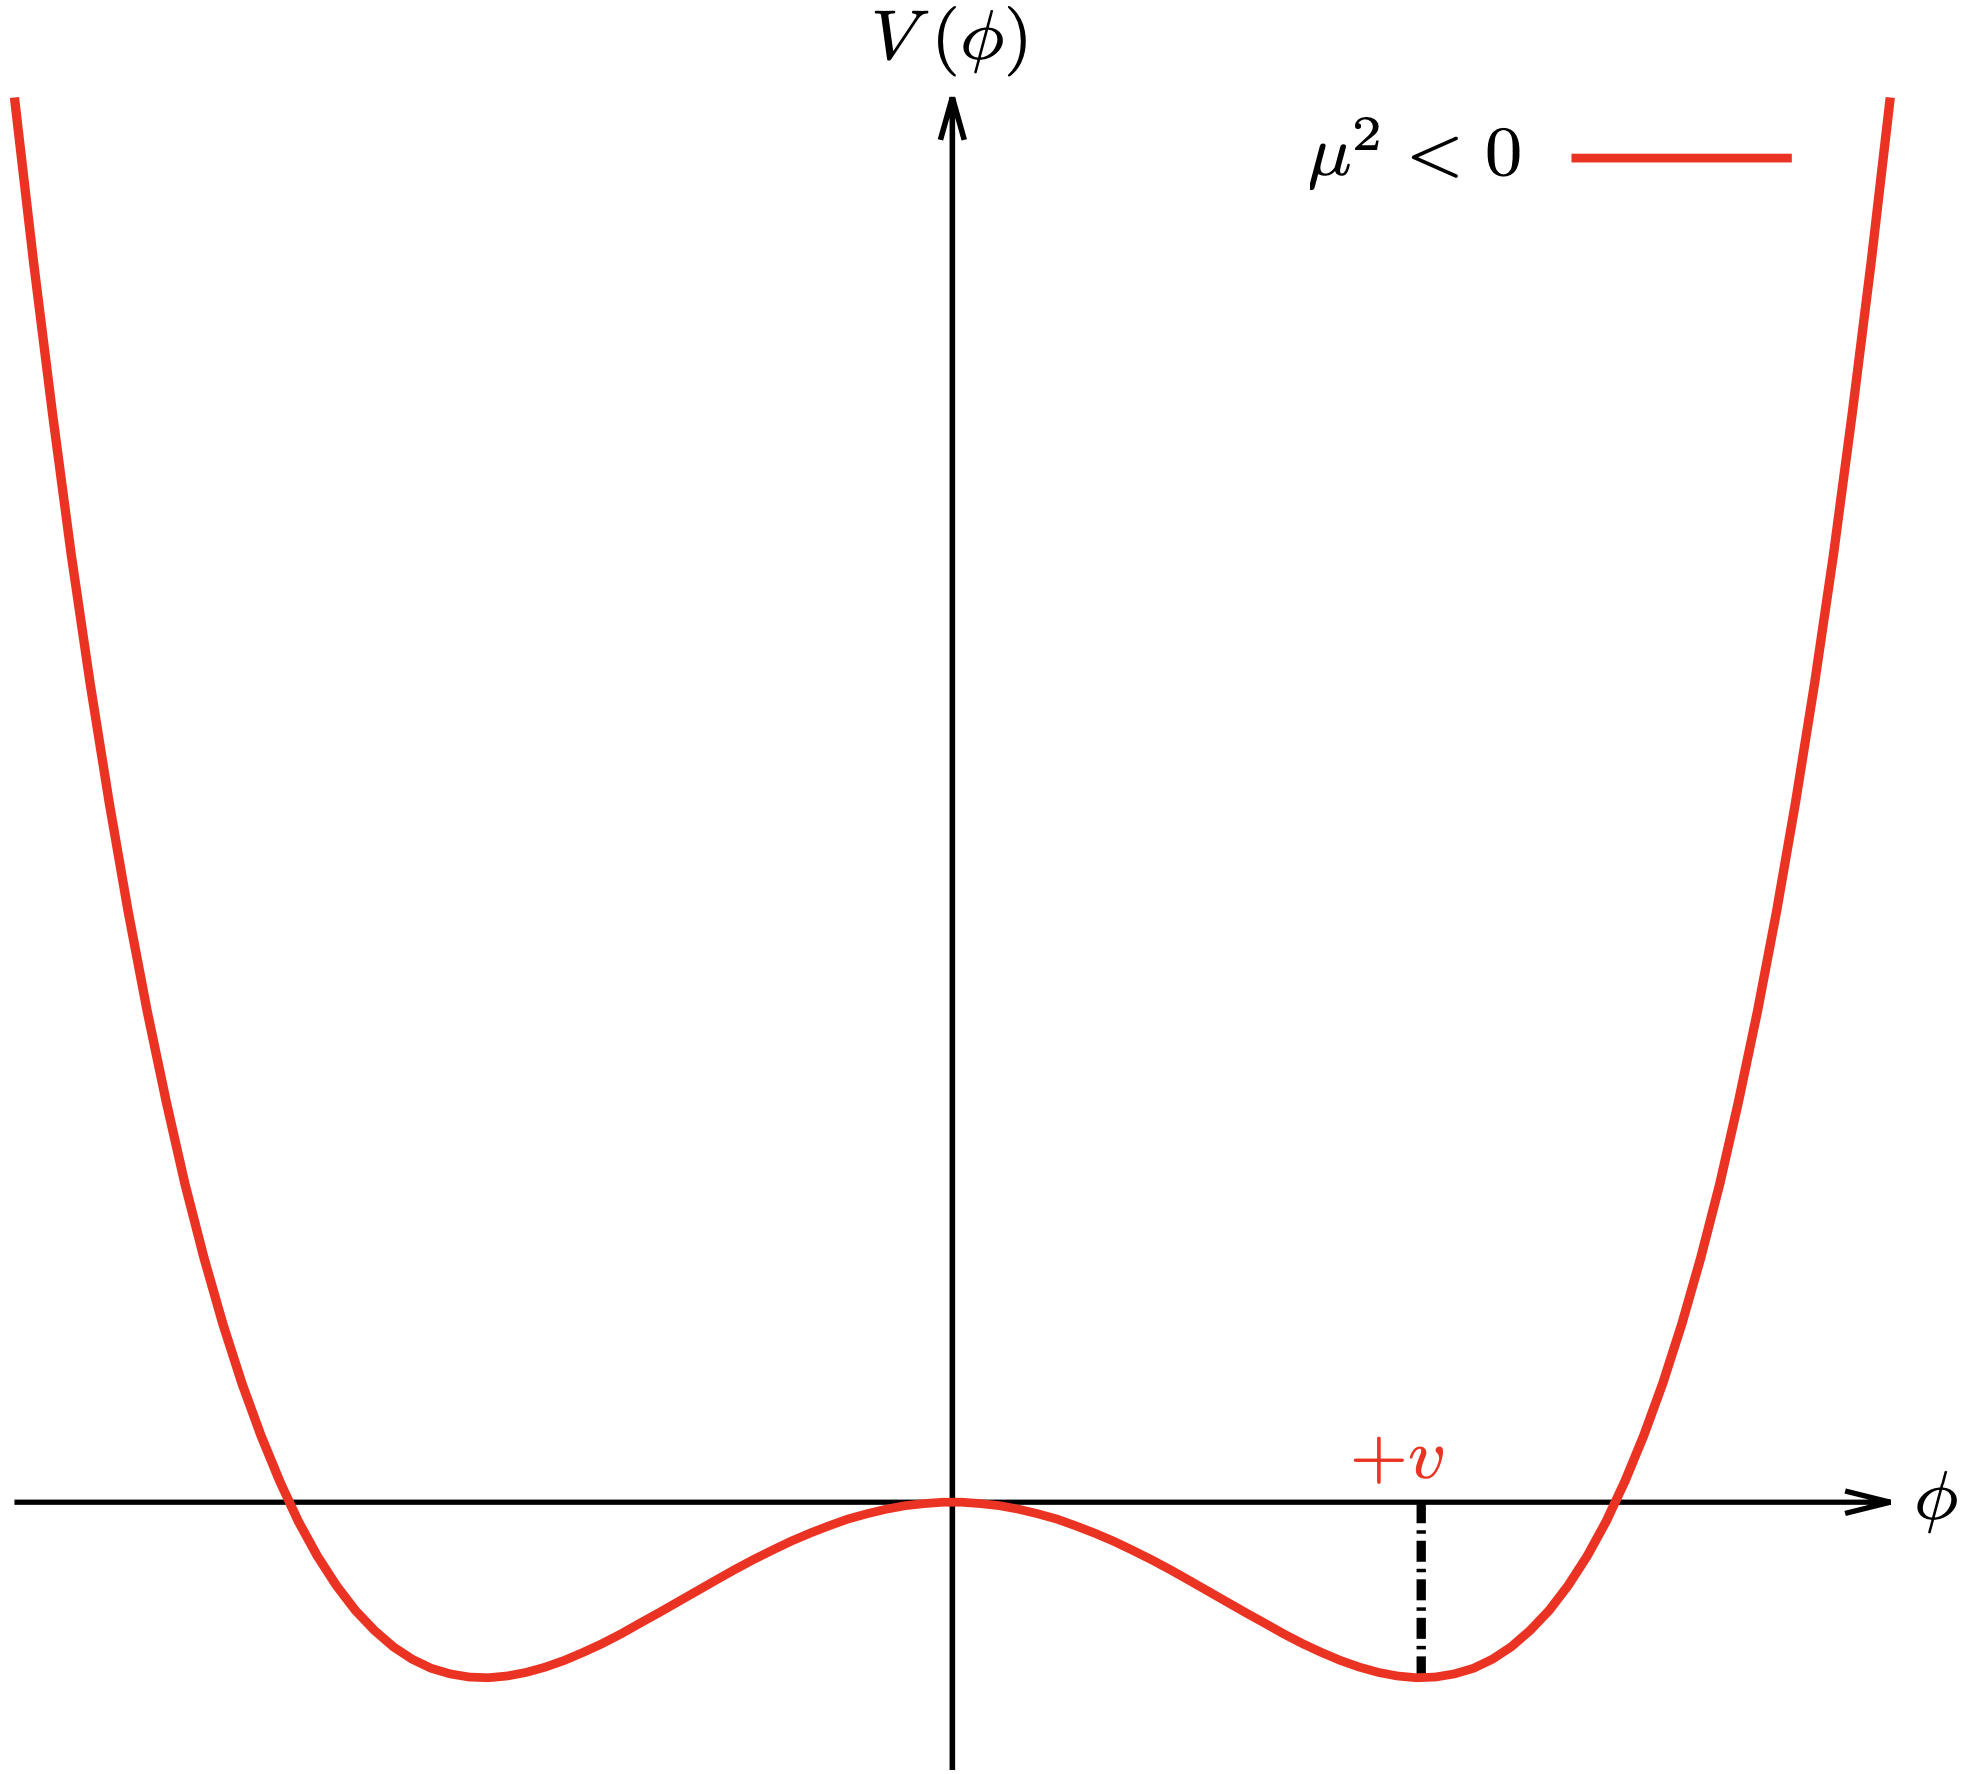
\includegraphics[width=.74\linewidth]{Chapter1/Higgs_V_muminus}
%  \caption{}
%  \label{fig:Chap1:SM:HiggsMechanism:PotentialExample:Negative}
%\end{subfigure}
%\caption{The potential $V(\phi)$ of Lagrangian \ref{eq:chap1:HiggsMechanism:Example} for(a) $\mu^{2}$ positive and (b) negative.}  
%\label{fig:Chap1:SM:HiggsMechanism:PotentialExample}
%\end{figure}
%Expanding the field around the minima at $\phi_{i} =(0,0,0,v)$, the $\mathcal{L}$ becomes:
%\begin{equation}
%\begin{split}
%	\mathcal{L} 	&= \frac{1}{2}\partial_{\mu}\sigma\partial^{\mu}\sigma + \mu^{2}\sigma^{2} -\sqrt{\mu^{2}\lambda}\sigma^{3} -\frac{1}{4}\lambda^{4} \\
%				& + \frac{1}{2}\partial_{\mu}\pi_{i}\partial^{\mu}\pi_{i} -\frac{1}{4}\lambda (\pi_{i}\pi_{i})^{4} - \lambda v \pi_{i}\pi_{i}\sigma - \frac{1}{2}\pi_{i}\pi_{i}\sigma^{2} \, ,
%\end{split}
%\end{equation}
%where $i$ runs from 1 to 3. Here $\sigma = \phi_{4}-v$ and $\pi_{i} = \phi_{i}$ are new boson fields, being the latter massless and the former with a mass of $m_{\sigma}^2 = -2\mu^{2}$.
%The new terms break the original symmetry because the symmetry of the Lagrangian is not longer a symmetry of the vacuum, it has been spontaneously broken.
%One massive $\sigma$ boson and three massless $\pi_{i}$ bosons with a residual $O(3)$ symmetry have appeared. This is a consequence of the Goldstone theorem which states that 
%``for a continuous symmetry group $\mathcal{G}$ spontaneously broken down to a subgroup $\mathcal{H}$, the number of broken generators is equal to the number of massless scalars 
%that appear in the theory''~\cite{Goldstone:1962es}. Therefore, since the $O(N)$ group has $N(N-1)/2$ generators, the $O(N-1)$ has $(N-1)(N-2)/2$ and, hence, $N-1$ Goldstone bosons
%appear. The example shown is for $N=4$.


\paragraph{The Higgs mechanism in the SM for bosons}\mbox{}\\
The Goldstone theorem  states that 
``for a continuous symmetry group $\mathcal{G}$ spontaneously broken down to a subgroup $\mathcal{H}$, the number of broken generators is equal to the number of massless scalars  that appear in the theory''~\cite{Goldstone:1962es}.
To apply this mechanism to the SM, it is necessary to generate mass for the \PWplus, \PWminus and \PZ bosons while keeping the photon massless. 
%The Higgs mechanism is based on the general idea of spontaneous symmetry breaking, meaning that for a system the ground state is not equivalent to a
%fully symmetric state. Implying that the systems evolves from a ground state which is not invariant under its full symmetry group.
To do so, the EW symmetry group $SU(2)_\text{L} \times U(1)_\text{Y}$ has to be broken into a $U(1)$ subgroup describing electromagnetism. 
A gauge-invariant interaction that gives masses to fermions without mixing chiral components
is introduced by defining a $SU(2)$ isospin doublet of complex scalar field with hypercharge $\text{Y}=1$:
\begin{equation*}
	\Phi = \begin{pmatrix} \phi^+ \\ \phi_0 \end{pmatrix}\, .
\end{equation*}
Being $\phi^+$ positively charged and $\phi^0$ neutral. The Lagrangian $\mathcal{L}_{\text{Higgs}}$ has to be added to the $\mathcal{L}_{\text{EW}}$ in equation~\ref{eq:chap1:EW:FinalL}.
\begin{equation*}\label{eq:chap1:HiggsMechanism:HiggsLagrangianA}
	\mathcal{L}_{\text{Higgs}} = (D_{\mu} \Phi)^{\dagger}(D^{\mu} \Phi) - V(\Phi) \textrm{ where } V(\Phi) = \mu^{2}\Phi^{\dagger} \Phi + \lambda (\Phi^{\dagger} \Phi)^{2}\, ,
\end{equation*}
with $\lambda >0$ required for vacuum stability. When $\mu^{2}>0$, the minimum of the potential occurs when both fields ($\phi^+$ and $\phi^0$) are at zero. If $\mu^{2}<0$, the 
minimum of the potential has an infinite number of degenerate states that satisfy $\Phi^{\dagger} \Phi = \mu^{2}/2\lambda$ and the physical vacuum state will correspond 
to any particular point on the circle of Figure~\ref{fig:Chap1:SM:HiggsMechanism:Potential}.
Having to choose a particular point breaks the global $U(1)$ symmetry of the Lagrangian. Without loss of generality, in this scenario, the ground state $\Phi_{0}$ can be chosen to be:
\begin{equation*}
	\Phi_{0} = \frac{1}{\sqrt{2}}\begin{pmatrix} 0 \\ v \end{pmatrix} \textrm{ where } v = 2\sqrt{\frac{\mu^{2}}{\lambda}}\, .
\end{equation*}
being $v$ the vacuum expectation value. This defines the already mentioned circle in the minimum of $V(\Phi)$ in the $\mu^{2}<0$ scenario.

\begin{figure}
    \centering
    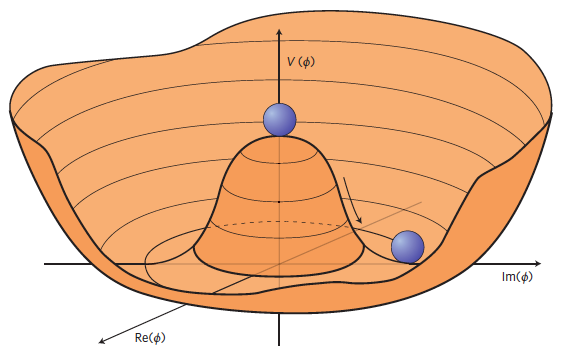
\includegraphics[width = 0.7\textwidth]{Chapter1/HiggsPotential}
    \caption{An illustration of the Higgs potential $V(\Phi)$ in the case of $\mu^{2}<0$~\cite{Bass:2764481}. Choosing any particular point in the circle defined by $v$ spontaneously breaks the $U(1)$ rotational symmetry. This type of potential is
    frequently called ``Mexican hat''.}
    \label{fig:Chap1:SM:HiggsMechanism:Potential}
\end{figure}

The Lagrangian density must be formulated in terms of deviations from one of these
ground states. This can be done by introducing an excitation, $h(x)$, that can be understood
as a small deviation of the field from the ground state. 
Accordingly, the fields can be expanded around the minimum as:
%\begin{equation*}
%	\Phi = \frac{1}{\sqrt{2}} \begin{pmatrix} 0 \\ v+h(x) \end{pmatrix} exp\{  i \chi(x)\}\, .
%\end{equation*}
%The new field $\chi(x)$ can be set to zero in the so called ``unitary gauge''.
\begin{equation}\label{eq:chap1:HiggsMechanism:SymmetryBreaking}
	\Phi = \frac{1}{\sqrt{2}} \begin{pmatrix} 0 \\ v+h(x) \end{pmatrix} \, ,
\end{equation}
%Expanding the covariant derivative of the $\mathcal{L}_{\text{Higgs}}$:
%\begin{equation*}\label{eq:chap1:HiggsMechanism:Covariant}
%\begin{split}
%	 (D_{\mu} \Phi)^{\dagger}(D^{\mu} \Phi) 	&=\left\lvert \left( \partial_{\mu} + ig \frac{\tau^{k}}{2} \PW_{\mu}^{k} (x)+ ig' \frac{y}{2} B_{\mu} \right)\right\rvert^{2} \\
%									&= \frac{1}{2} \left\lvert \begin{pmatrix}  \partial_{\mu} +i\frac{1}{2}(gW^{3}_{\mu}+g'\frac{y}{2} B_{\mu}) && i\frac{g}{2}(W^{1}_{\mu}-iW^{2}_{\mu}) \\
%									i\frac{g}{2}(W^{1}_{\mu}-iW^{2}_{\mu}) && \partial_{\mu} -i\frac{1}{2}(gW^{3}_{\mu}-g'\frac{y}{2} B_{\mu})
%									 \end{pmatrix}  \begin{pmatrix} 0 \\ v+h \end{pmatrix}\right\rvert ^{2} \\
%									 &= \frac{1}{2}(\partial_{\mu} h)^{2} + \frac{1}{8}(v+h)^{2}|W^{1}_{\mu}-iW^{2}_{\mu}|^{2} \\
%									 &+ \frac{1}{8}(v+h)^{2}|gW^{3}_{\mu}-g'B_{\mu}| +(\textrm{interaction terms}) \, ,
%\end{split}
%\end{equation*} %source: https://arxiv.org/pdf/1709.10508.pdf
%where the $\tau_k$ with $k={1,2,3}$ are the Pauli Matrices. In this equation there are terms mixing the $W^{3}$ and the $B_{\mu}$ fields that, by using the physical fields defined in equation~\ref{eq:chap1:EW:ZmuAmu}, should disappear since the physical bosons do not mix. Applying the Relation \ref{eq:chap1:EW:ZmuAmu} into the covariant derivative, 
and the covariant derivative takes the form:
\begin{equation*}
	(D_{\mu} \Phi)^{\dagger}(D^{\mu} \Phi) = \frac{1}{2}+\frac{g^2v^2}{4}W^{+}_{\mu} W^{-\, \mu} + \frac{g^{2} v^{2}}{8 \textrm{cos}^{2}\theta_{W}}Z_{\mu}Z^{\mu} \, , %+ 0 A_{\mu}A^{\mu}
\end{equation*}
where $\theta_{W}$ is the weak mixing angle, which is measured to be 
\mbox{$\textrm{sin}^{2} \theta_{W} = 0.2310\pm0.0005$}~\cite{CMS:2018ktx}.
By doing this, the \PWplus, \PWminus and \PZ bosons have finally acquired mass. Through the Higgs mechanism, their masses within the SM are:
\begin{align*}
	M_{\PW} = \frac{1}{2}gv 	&&  	\text{and}	&& M_{\PZ} = \frac{1}{2}\frac{gv}{\textrm{cos}\,\theta_{W}}\, .
\end{align*}
Additionally, a new scalar field $h(x)$ has appeared with its correspondent mass term, the Higgs field. Note that the $h(x)$ was introduced as a perturbation from the ground
state of the Higgs potential $V(\Phi)$, so the Higgs boson can be understood as an excitation of the Higgs potential. Apart from couplings to the electroweak gauge
fields, the Higgs field also has self-interaction vertices. The mass of this boson is $m_{\PHiggs}=\sqrt{2}\mu$.

With this covariant term, the Higgs Lagrangian density of the system is obtained:
%\begin{equation*}\label{eq:chap1:HiggsMechanism:HiggsLagrangianB}
%\begin{split}
%	\mathcal{L}_{\text{Higgs}} 	&= \frac{1}{2} (\partial_{\mu}h) (\partial^{\mu}h) + \frac{g}{4}(v+h)^{4}\PW_{\mu}\PW^{\mu} + \frac{g^{2}}{8 \textrm{cos}^{2}\theta_{W}}(v+h)^{2}\PZ_{\mu}\PZ^{\mu} \\
%					&+\frac{\mu^{2}}{2}(v+h)^{2} - \frac{\lambda}{16}(v+h)^{4}
%\end{split}
%\end{equation*}
%and expressing it in terms of the boson masses and coupling parameters, it can be written as:
\begin{equation}\label{eq:chap1:HiggsMechanism:HiggsLagrangianC}
\begin{split}
	\mathcal{L}_{\text{Higgs}} 	&= \frac{1}{2} (\partial_{\mu}h) (\partial^{\mu}h)  - \frac{1}{2}m^{2}_{\PHiggs}h^{2}+\frac{1}{2}m_{\PW}\PW_{\mu}\PW^{\mu}+\frac{1}{2}m_{\PZ}\PZ_{\mu}\PZ^{\mu} + g m_{\PW} h \PW_{\mu}\PW^{\mu} \\
					&+ \frac{g^{2}}{4}\PW_{\mu}\PW^{\mu} + g \frac{m_{\PZ}}{2 \textrm{cos}\,\theta_{W}} h \PZ_{\mu}\PZ^{\mu} - g^{2}\frac{1}{4 \textrm{cos}^{2}\theta_{W}}h^{2}\PZ_{\mu}\PZ^{\mu} 
					 -g \frac{m^{2}_{H}}{4 m_{\PW}}h^{3} \\
					& -g^{2}\frac{m^{2}_{H}}{32 m^{2}_{\PW}}h^{4}+\textrm{const.}
\end{split}
\end{equation}
As can be seen in the Lagrangian in equation~\ref{eq:chap1:HiggsMechanism:HiggsLagrangianC}, the coupling strengths of the \PW and \PZ 
fields to the Higgs field are proportional to $m_{\PW}$ and $m_{\PZ}$, respectively.
%This why it is said that the more a fundamental particle interacts with the Higgs boson, the more massive it is.
% It is not that the particles that have more mass interact more with the Higgs fields but the 
% other way round: the particles that interact more with the Higgs fields have more mass, i.e. the interaction with the Higgs proceeds the mass of the particles.

%Another way to interpret this is by understanding the mass as the tendency to resist movement, therefore, if a particle interacts strongly with the Higgs field, it is more difficult for that particle to 
%move and hence this particle is more massive. The Higgs field acts as a viscosity. 

\paragraph{The Higgs mechanism in the SM for fermions}\mbox{}\\ %Source: Book - Modern Particle Physics - Mark Thompson (me lo prestó Stef)
The Higgs mechanism for spontaneous symmetry breaking of the $SU(2)_\text{L} \times U(1)_\text{Y}$ gauge group of the SM generates the masses of the \PWpm and \PZ bosons.
For originating the mass of the fermions without violating the EW gauge symmetry a similar procedure is carried but taking into account that the left-handed particles transform differently 
than the right-handed. To do so, additional terms including the Yukawa couplings are added into the Lagrangian. These terms are of the form:
\begin{align*}
\mathcal{L}_{\text{Yukawa,} f}=-y_{f}(\bar{\chi}_{L}^f \Phi \chi_\text{R}^{f} + \bar{\chi}_{\text{R}}^f \Phi^{\dagger} \chi_\text{L}^{f} )\, \text{, with }\, \Phi = \begin{pmatrix} \phi^+ \\ \phi_0 \end{pmatrix} 
\end{align*}
where the $f$ superindex runs over all quarks and charged leptons. %It is usual to express the second part of the sum just as ``plus hermitic conjugate'' (``+ h.c.''). Note that the hermitic conjugate part
%is necessary to ensure that expression fulfils the requirement for a hermitian operator to be self-adjoint in a complex Hilbert space.
The different $y_f$ constants are known as Yukawa couplings of the particle $f$ to the Higgs field. The Higgs doublet is denoted by $\Phi$.
For the electron $SU(2)$ doublet, the element with this coupling can be written as:
\begin{equation}\label{eq:chap1:HiggsMechanism:ElectronDoubletLagrangian}
\mathcal{L}_{\Pe} = - y_{\Pe} \left[ (\bar{\Pnu}_{\Pe} \bar{\Pe})_{\text{L}} \begin{pmatrix} \phi^{+} \\ \phi^{0} \end{pmatrix} \Pe_{\text{R}} + \bar{\Pe_{\text{L}}} (\phi^{+*} \phi^{0*})\begin{pmatrix} \Pnu_{\Pe} \\ \Pe \end{pmatrix}_{\text{L}} \right] \, .
\end{equation}
Here, $y_{e}$ is the Yukawa coupling of the electron to the Higgs boson. 
After spontaneously breaking the symmetry as it is done 
in equation~\ref{eq:chap1:HiggsMechanism:SymmetryBreaking}, and the 
$y_{\Pe}$ is set to $y_{\Pe}=\sqrt{2}\,m_{\Pe}/v$ where $m_{\Pe}$ is the observed 
electron mass, 
 the Lagrangian in equation~\ref{eq:chap1:HiggsMechanism:ElectronDoubletLagrangian} becomes:
%\begin{equation}\label{eq:chap1:HiggsMechanism:ElectronBroken}
%\mathcal{L}_{\Pe} = \frac{-y_{\Pe}}{\sqrt{2}} v (\bar{\Pe}_{\text{L}}\Pe_{\text{L}} + \bar{\Pe}_{\text{L}}\Pe_{\text{L}}) + \frac{-y_{\Pe}}{\sqrt{2}} h (\bar{\Pe}_{\text{L}}\Pe_{\text{L}} + \bar{\Pe}_{\text{L}}\Pe_{\text{L}} )
%\end{equation}
%The $y_{\Pe}$ is not predicted by the Higgs mechanism, but can be chosen to be consistent with the observed electron mass ($m_{\Pe}$) so that $y_{\Pe}=\sqrt{2}\,m_{\Pe}/v$. Using this relation, the Lagrangian in \ref{eq:chap1:HiggsMechanism:ElectronBroken} becomes:
\begin{equation}\label{eq:chap1:HiggsMechanism:ElectronMassL}
\mathcal{L}_{\Pe} = -m_{\Pe} \bar{\Pe}\Pe - \frac{m_{\Pe}}{v}\bar{\Pe}\Pe h
\end{equation}
The first element of the Lagrangian in equation~\ref{eq:chap1:HiggsMechanism:ElectronMassL} gives mass to the electron and gives rise to the coupling of the electron to the Higgs fields in its non-zero vacuum expectation. 
The second term represents the coupling of the electron and the Higgs boson itself.

The non-zero vacuum expectation value occurs only in the neutral part of the Higgs doublet due to the form 
in the ground state in equation~\ref{eq:chap1:HiggsMechanism:SymmetryBreaking}. This implies that the combination $\bar{\chi}_{\text{L}}^f \Phi \chi_\text{R}^{f} + \bar{\chi}_{\text{L}}^f \Phi^{\dagger} \chi_\text{L}^{f}$ can only generate
masses for the fermions in the lower component of an $SU(2)$ doublet, i.e. the charged leptons and the down type quarks. Putting aside the procedure to give mass to the up-type quarks,
this explains why the neutrinos do not get mass through the Higgs mechanism.

%For the up-type quarks, a gauge invariant term can be constructed from $\bar{\chi}_{\text{L}}^f \Phi_{c} \chi_\text{R}^{f} + \bar{\chi}_{\text{L}}^f \Phi_{c}^{\dagger} \chi_\text{L}^{f}$:
%\begin{equation*}%\label{eq:chap1:HiggsMechanism:UpType}
%\mathcal{L}_{\Pup} = y_{\Pup} (\bar{\Pup} \bar{\Pdown})_{\text{L}} \begin{pmatrix} -\phi^{0*} \\ \phi^{-} \end{pmatrix} \Pup_{\text{L}} + \textrm{h.c.}
%\end{equation*}

For up-type quarks, after applying the symmetry breaking and using $y_{\Pup}=\sqrt{2}\,m_{\Pup}/v$, the Lagrangian density takes the form:
%\begin{equation*}\label{eq:chap1:HiggsMechanism:UpTypeBroken}
%\mathcal{L}_{\Pup} = \frac{-y_{\Pup}}{\sqrt{2}} v (\bar{\Pup}_{\text{L}}\Pup_{\text{L}} + \bar{\Pup}_{\text{L}}\Pup_{\text{L}}) + \frac{-y_{\Pup}}{\sqrt{2}} h (\bar{\Pup}_{\text{L}}\Pup_{\text{L}} + \bar{\Pup}_{\text{L}}%\Pup_{\text{L}} )
%\end{equation*}
%with a Yukawa coupling between the up quark and the boson $y_{\Pup}=\sqrt{2}\,m_{\Pup}/v$, resulting in:
\begin{equation*}%\label{eq:chap1:HiggsMechanism:ElectronMassL}
\mathcal{L}_{\Pup} = -m_{\Pup} \bar{\Pup}\Pup - \frac{m_{\Pup}}{v}\bar{\Pup}\Pup h .
\end{equation*}

%Therefore, for Dirac fermions, mass terms that let the Lagrangian invariant under local gauge transformations can be constructed from
%\begin{align*}%\label{eq:chap1:HiggsMechanism:ForFermions}
%\mathcal{L} = -y_{f}\left[\bar{\chi}_{\text{L}}^f \Phi \chi_\text{R}^{f} + (\bar{\chi}_{\text{L}}^f \Phi \chi_\text{L}^{f} )^{\dagger} \right] && \textrm{ or } && \mathcal{L} = y_{f}\left[\bar{\chi}_{\text{L}}^f \Phi_{c}\chi_\text{R}^{f} + (\bar{\chi}_{\text{L}}^f \Phi_{c} \chi_\text{L}^{f} )^{\dagger}\right] .
%\end{align*}
%The left Lagrangian is used for the leptons and down-type quarks, while the right one is used for the up-tupe quarks. 
These elements give rise not only to the mass of the fermions but also to the interaction
strengths between these fermions and the Higgs boson. The Yukawa coupling of the fermions to the Higgs field is given by:
\begin{equation}\label{eq:chap1:HiggsMechanism:YukawaCoupling}
	y_{f} = \sqrt{2} \, \frac{m_{f}}{v} \, ,
\end{equation}
where the Higgs vacuum expectation value is fixed by the Fermi coupling $G_{F}$ and is measured to be $v = \sqrt{2}\,G_{F} \approx 246.22$~GeV. The $G_{F}$ 
is measured from the antimuon ($\APmuon$) lifetime measurement~\cite{MuLan:2010shf}. 
%The $G_{F}$ is also used to determine the magnitude of the elements in the CKM matrix.

The value of fermionic masses is not predicted by the SM but obtained through experimental observations.
Given the measured top-quark mass, $\mtop = 172.76 \pm 0.30$~GeV~\cite{Workman:2022ynf}, it is of particular interest the Yukawa coupling of the top quark to the Higgs field (\yt), which is almost exactly equal to one. %~\cite{pdgTop}
 It is important to verify this because deviation of the measured \yt from the SM prediction would be proof of new physics.
 The object of this thesis is precisely the measurement of a process whose cross-section is directly related to \yt.
 %phenomena beyond the SM that could provide an 
%answer to several open questions concerning the fundamental interactions of elementary particles.
%For the top quark, the Yukawa coupling, $y_t$ almos exactly the unity. 


%https://www.youtube.com/watch?v=2TYFNOArnYo&t=2006s 






%%%%%%%%%%%%%%%%%%%%%
%                  Charge Parity                    %
%%%%%%%%%%%%%%%%%%%%%
%\subsection{Charge-Parity}
%\label{sec:chap1:CP_Violation}
% https://www.damtp.cam.ac.uk/user/tong/qft/four.pdf   <- p. 93-95 or PT and 96-96 C
% Parity and Charge conjugation: https://ocw.mit.edu/courses/physics/8-323-relativistic-quantum-field-theory-i-spring-2008/lecture-notes/ft1ls06p_08.pdf
% Intro of this paper: https://arxiv.org/pdf/2201.02385.pdf
% ATLAS: https://atlas.cern/updates/briefing/symmetry-breaking-higgs-boson <- Searching for new sources of matter–antimatter symmetry breaking in Higgs boson interaction with top quarks

%\pablo{Probably, this section is gonna be absorbed by \ref{sec:chap1:EW}}


%%%%%%%%%%%%%%%%%%%%%
%                        Wrap up                        %
%%%%%%%%%%%%%%%%%%%%%
\section{Remarks about the limitations of the Standard Model}
\label{sec:chap1:Wrapup}
%Once the gauge symmetries and the fields with their gauge quantum numbers are specified, the Lagrangian of
%the SM is fixed by requiring it to be invariant under local gauge transformations, and renormalisable. 
%The SM Lagrangian can be divided into several pieces.

%Perhaps the ultimate and definitive (if talking about definitive makes any sense) theory of particle physics 
%is a simple equation with a small number of free parameters. Meanwhile, the SM is here, and while it is not
But the SM is not  
the ultimate theory, it is unquestionably one of the greatest successes of modern physics.
Despite its achievements, many questions remain unsolved.


\subsection{The parameters of the Standard Model}
\label{sec:chap1:Wrapup:ParamsOfSM}
The SM contains 25 free parameters that must be determined through experimentation. 
These are the masses of the 12 fermions, %(assuming colour variations and antiparticles that are not viewed as 
%separate fermions) or, more precisely, the 12 Yukawa couplings to the Higgs field, % ($m_{\nu_{1}}, m_{\nu_{2}}, m_{\nu_{3}}, m_{e}, m_{\mu}, m_{\tau},
%	m_{u}, m_{d}, m_{c}, m_{s}, m_{t} \textrm{ and }  m_{b}$)
%	
%\begin{equation*}
%	m_{\nu_{1}}, m_{\nu_{2}}, m_{\nu_{3}}, m_{e}, m_{\mu}, m_{\tau},
%	m_{u}, m_{d}, m_{c}, m_{s}, m_{t} \textrm{ and }  m_{b}
%\end{equation*} 
the three coupling constants for describing the strength of the gauge interactions ($g, g' \textrm{ and } g_{s}$)
%\begin{equation*}
%	g, g' \textrm{ and } g_{s}
%\end{equation*} 
 and the two parameters describing the Higgs potential ($\mu$ and $\lambda$) or, equivalently, its vacuum  
expectation value $v$, and the Higgs-boson mass $m_{h}$.
%\begin{equation*}
%	v \textrm{ and }m_{h}
%\end{equation*} 
Finally, there are three mixing angles and the complex phase of the CKM matrix and four 
Pontecorvo--Maki--Nakagawa--Sakata matrices, %($\theta_{12}, \theta_{13}, \theta_{23}, \rho_{13}, \theta'_{a}, \theta'_{b}, \theta'_{c} \textrm{ and }\theta'_{d}$)
which mix the neutrino-mass eigenstates with neutrino-flavour eigenstates~\cite{Maki:1962lba, Pontecorvo:1957qd}.
%\begin{equation*}
%	\theta_{12}, \theta_{13}, \theta_{23}, \rho_{13}, \theta'_{a}, \theta'_{b}, \theta'_{c} \textrm{ and }\theta'_{d}
%\end{equation*} 

From the 25 free parameters of the SM, 14 are associated with the Higgs field, eight with the flavour sector and
only three with the gauge interactions. This emphasises the crucial significance of precisely measuring and 
comprehending the properties of the Higgs particle.

%%%%%%%%%%%%%%%%%%%%%%%%
%                  Problems with the SM                  %
%%%%%%%%%%%%%%%%%%%%%%%%
\subsection{Limitations of the Standard Model}
\label{sec:chap1:SM_problems}
While the SM is an extremely successful theory that has passed rigorous testing %, this is not the end of the story, since
there are several limitations of the SM and a variety of phenomena that it does not explain. %The SM 
%does not explain all questions in the universe and, hence, physicists continue looking for more general theories 
%to better explain the universe.  There is a long list of issues with the SM but, 
In the following pages, the most relevant issues with the SM are described.

\paragraph{Matter--antimatter asymmetry}\mbox{}\\
In principle, the Big Bang should have produced an equal amount of matter and antimatter 
which would all have then annihilated, leaving behind an empty universe filled with electromagnetic radiation.
 However, everything that is observed nowadays constituted of matter, from the tiniest life forms 
 on Earth to the greatest celestial objects. In comparison, there is not a lot of antimatter around. 

By looking at the cosmic microwave background (CMB) radiation, which contains the residual \Pgamma of the Big Bang, researchers 
have determined that there was a symmetry between the matter and antimatter content in the early universe. 
For every $3 \times 10^{9}$ antimatter particles, there were $3 \times 10^{9}$ and 1 matter particle.
The matter and antimatter annihilated and produced the CMB and the remaining 1 part turned into all the 
stars and galaxies that are seen.  %The field of cosmology that studies the processes that produced an 
%asymmetry between leptons and antileptons in the very early universe is called leptogenesis.

Research carried out during the last few decades has revealed that the laws of nature do not equally apply to
matter and antimatter~\cite{Sakharov:1967dj}. So far, the only non-trivial difference between matter and 
antimatter found is the \CP asymmetry or \CP violation. 
However, the \CP asymmetry included in the SM and observed in the experiments is insufficient 
to explain the composition of the observable universe and, hence, extensive searches for new sources of \CP 
violation are being carried out.

In this context, the study in this thesis seeks for new \CP-violation sources. %As Section
%\ref{sec:Chap1:tHq} details, the observation of a cross-section 
% greater than the one predicted by the SM may imply
%that the associated production of a Higgs boson and a single top quark does not conserve \CP.


%Where is the antimatter? One could think about antimatter galaxies, in the end, matter and antimatter emit the same kind of radiation. But, since the 
%antimatter galaxy would be surrounded by anti-hydrogen halo, when the halo of a matter galaxy and the halo of an antimatter galaxy enter in contact,
%the electrons and positrons of the halo would annihilate each other producing gamma rays. This gamma rays have not been observed and, hence,
%the existence of antimatter galaxies is desecrated.




%\paragraph{Strong \CP problem}\mbox{}\\ %https://cds.cern.ch/record/2652742/files/CERN-THESIS-2018-297.pdf
%https://inspirehep.net/literature/2089044
%\pablo{Write some lines here}



\paragraph{Gravity}\mbox{}\\
Gravity is the first force that any person learns about and the one known by humankind for longer. 
The SM describes all fundamental interactions but gravity. %In Table~\ref{tab:Chap1:FundamentalInteractions},
%the four forces are presented along with the theories to describe them. 
%While QCD, QED and EW interactions are part of the SM, the GR is not. 
GR is a geometric theory that currently describes gravitation in modern physics.
Some of the suggested solutions to integrate gravitational interactions in the SM consist of
postulating a new force carrier particle, the ``graviton'', that mediates this interaction in a similar way to how the gauge bosons
were proposed. Other explanations state that gravity can only be described by a deeper theory in which the 
time--space structure is not flat but dynamic. 

\paragraph{Neutrino masses}\mbox{}\\
According to the SM, the neutrinos are massless, nevertheless, many experiments confirm that this is not 
true~\cite{KATRIN:2021uub}. This is due to a property of neutrinos that allows them to change their flavour 
while travelling through space, this feature is known as ``neutrino oscillations''. Each of the three neutrino flavours
(\Pnue, \Pnum, \Pnut)
is a linear combination of three discrete neutrino-mass eigenstates ($\Pnu_{i}$ with $i\in\{1,2,3\}$) with mass eigenvalues 
($m_i$). While the neutrino oscillation experiments could probe the squared neutrino-mass eigenvalues 
($\Delta m^{2}_{ij}$), both the total scale of the masses and the sign of $\Delta m_{ij}$ remain as some of the most 
relevant open questions in particle physics. %Regarding to the sign of $\Delta m_{ij}$, it is known that the mass of 
%$\Pnu_{2}$ is slightly higher than $\Pnu_{1}$ ($\Delta m^{2}_{21}\equiv m^{2}_{2} - m^{2}_{1} \sim 10^{-4}$~eV) but 
%for the third mass eigenstate it has not been measured yet whether it is greater (normal ordering) or lower (inverted 
%ordering) than the other two, as it is depicted in Figure~\ref{fig:Chap1:Neutrino_problem}. Nevertheless, 
%the absolute square difference is known ($\Delta m^{2}_{31}\equiv |m^{2}_{3} - m^{2}_{1}| \sim 10^{-3}$~eV). 

%\begin{figure}
%    \centering
%    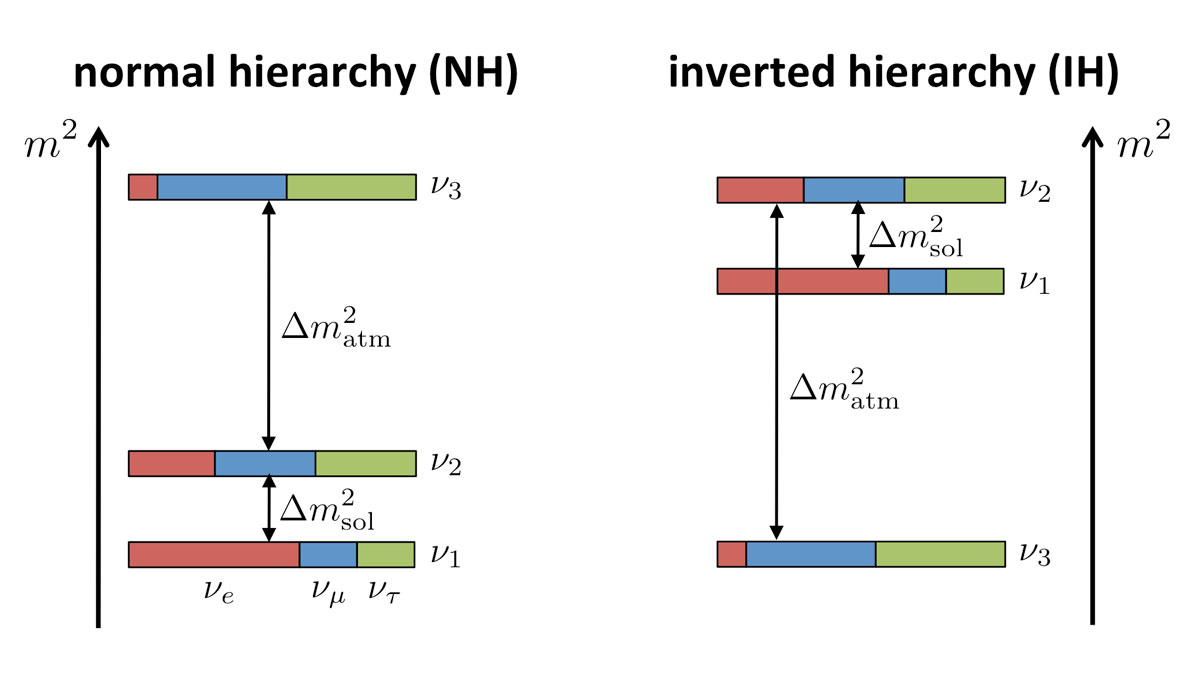
\includegraphics[width = 0.65\textwidth]{Chapter1/Neutrino_problem}
%    \caption{Two potential mass orderings of neutrinos are the normal ordering (normal hierarchy) and the inverted ordering (inverted hierarchy).}
%    \label{fig:Chap1:Neutrino_problem}
%\end{figure}

Non-zero neutrino masses opened an interesting portal beyond SM physics and, 
even though neutrinos are very elusive when it comes to detecting them, some 
next-generation experiments such as Dune~\cite{DUNE:2020lwj} target to set 
competitive and model-independent limits on neutrino masses. 

Regarding the nature of the neutrino mass, one could add mass terms to the SM as it is done in Section~\ref{sec:chap1:ParticleMasses:HiggsMechanism} 
for the up-type quarks but the origin of the neutrino masses is still not known. 
% It is possible that this mass comes from the Higgs mechanism, however, this is not clear.
Also, if neutrinos gained mass through Yukawa interaction, it would imply the presence of right-handed neutrinos, 
which has not been observed.

% Sterile neutrinos: special kind of neutrino that is proposed to explain some unexpected experimental results, but they have not been definitively discovered

% -  Neutrinos are the most elusive particles of the SM due to the difficulty of detect hem. However, some next generation experiments such 
% as Dune (Liquid argon detector) are very promising when it comes to set competitive and model independent limits on neutrino masses


\paragraph{Dark energy}\mbox{}\\
According to cosmological observations, the matter described by the SM only makes up around 5\% of the universe.
It turns out that roughly 68\% of the universe is made of dark energy, which is not considered by the SM.
%\begin{wrapfigure}{R}{0.5\textwidth}
%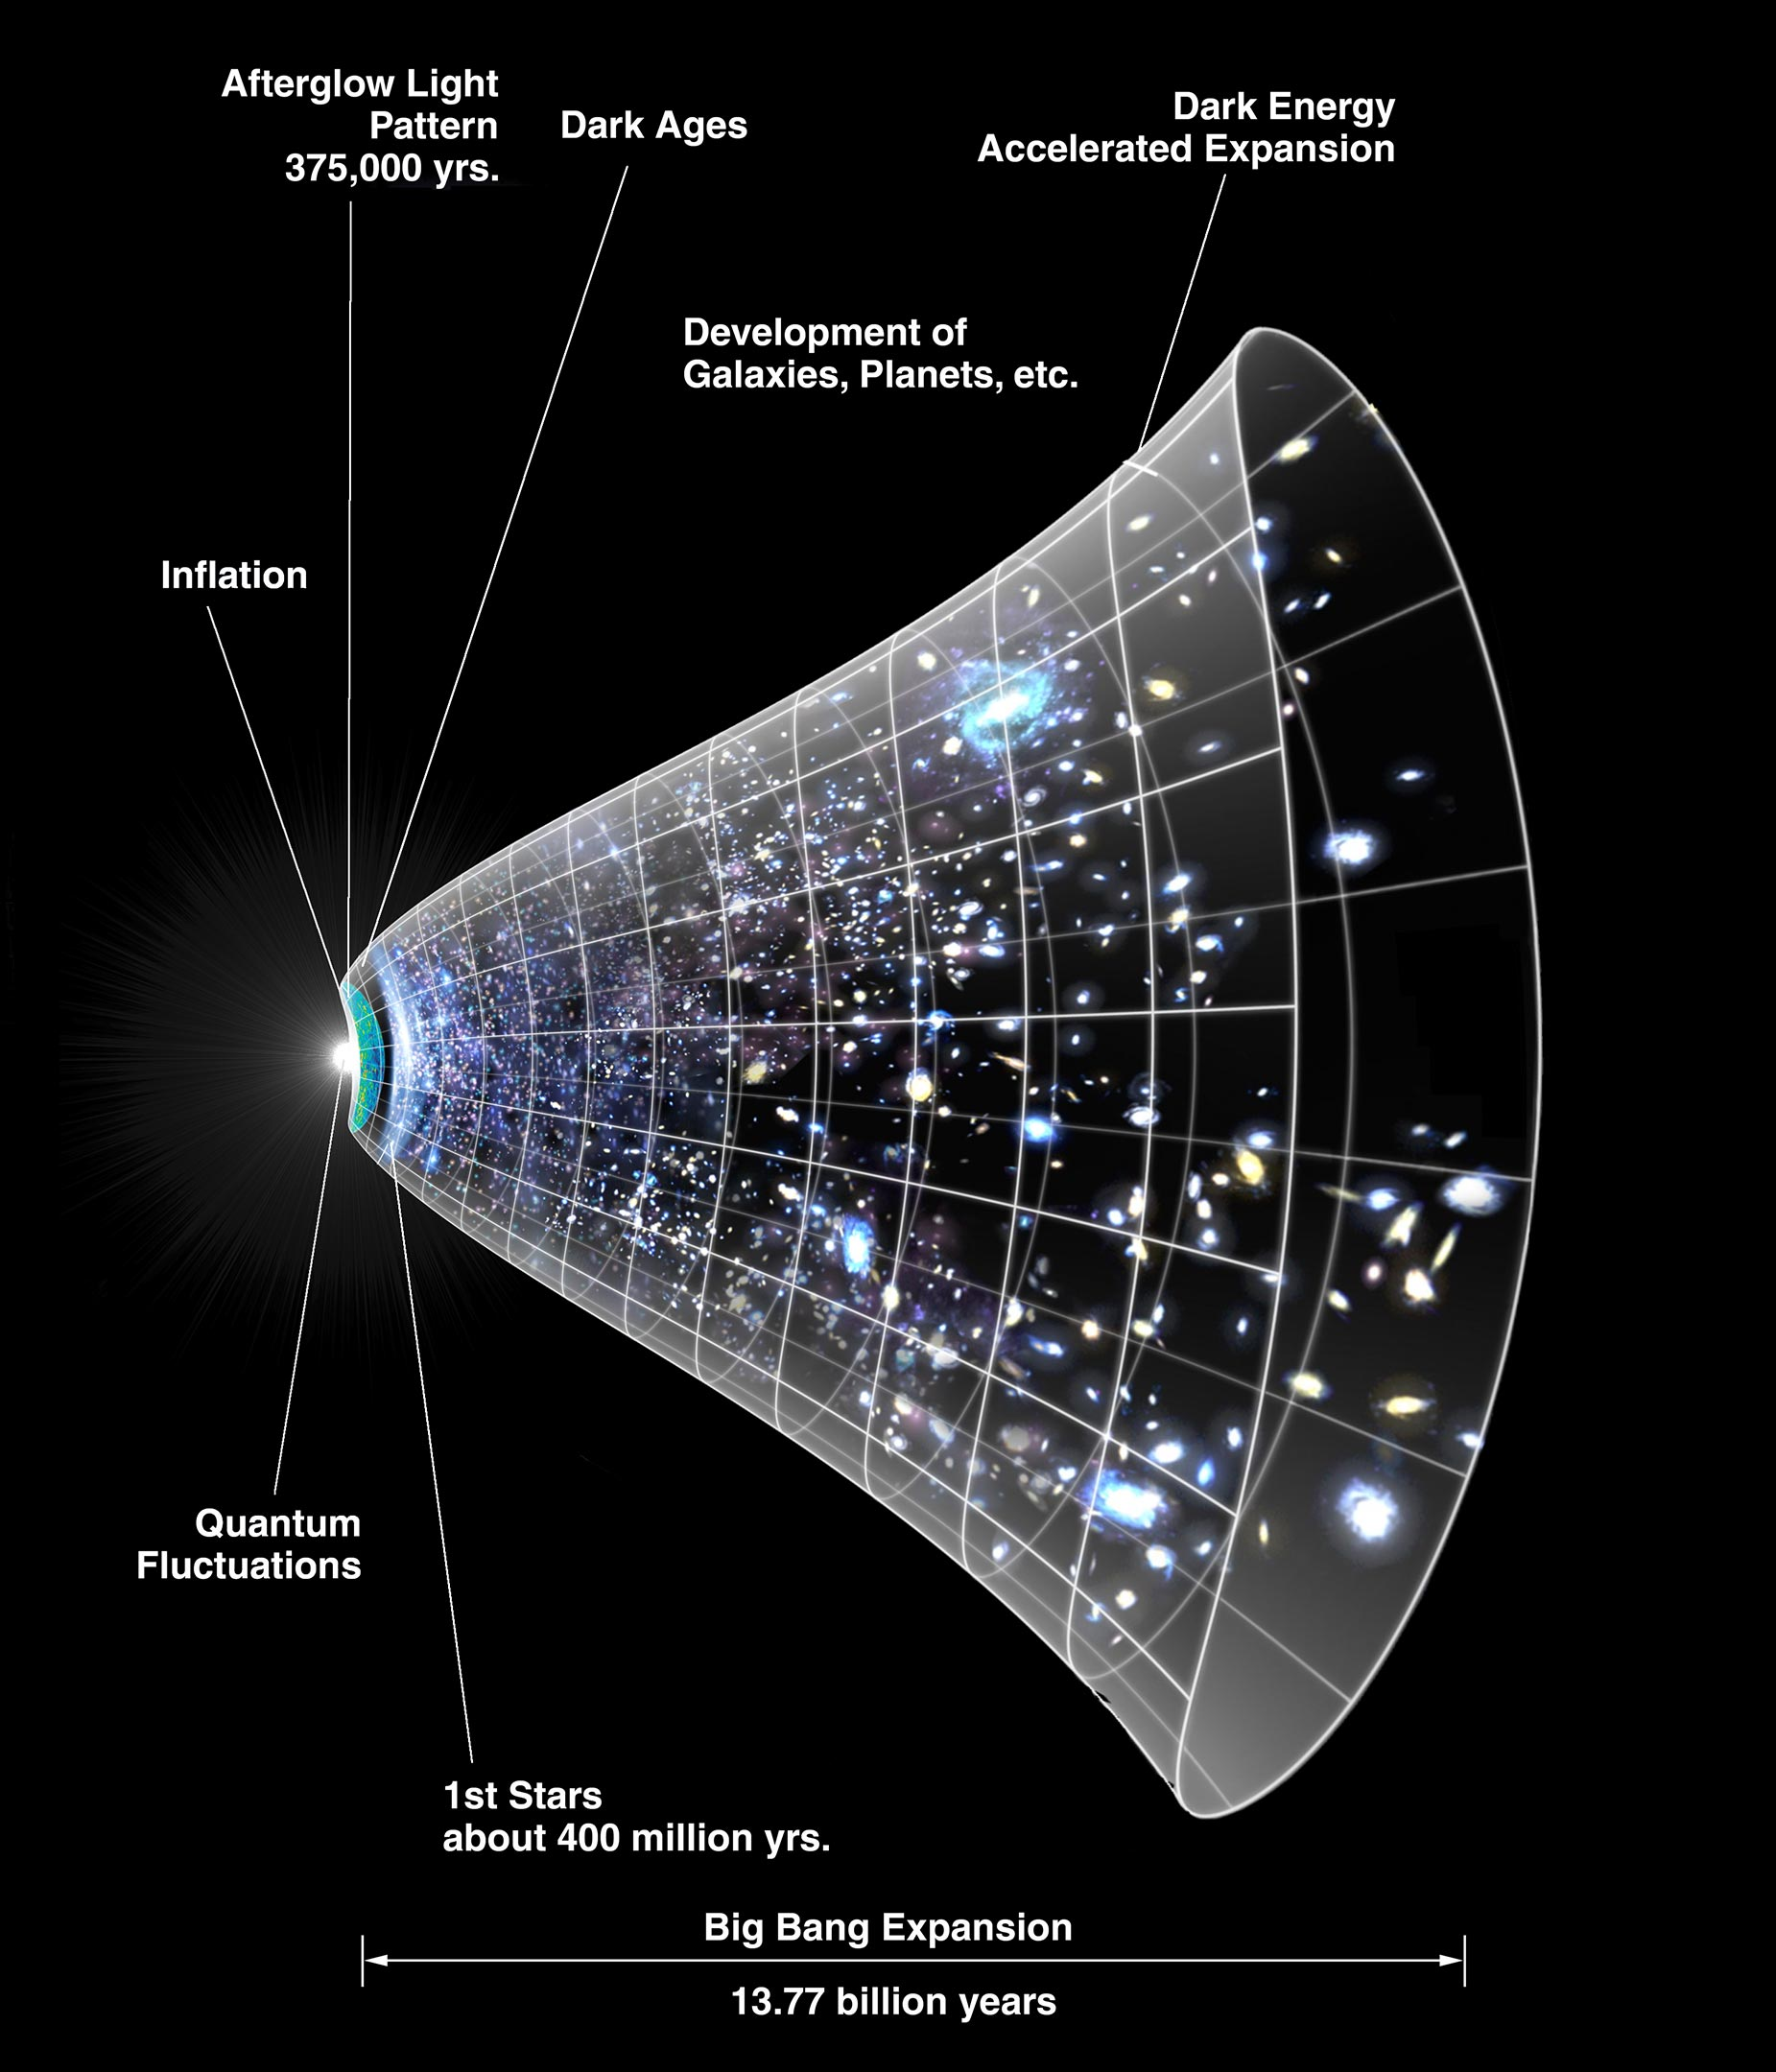
\includegraphics[width = 0.4\textwidth]{Chapter1/Limitations-UniverseExpansion}
%	\caption{The universe’s expansion over time. The dark-energy existence is suggested to explain this expansion.} %Credit: NASA/WMAP Science Team/ Art by Dana Berry
%	\label{fig:Chap1:UniverseExpansion}
%\end{wrapfigure} 

Dark energy is an unknown type of energy postulated to explain the observed accelerated expansion of the universe.
% as Figure~\ref{fig:Chap1:UniverseExpansion}.
This expansion is dominated by a spatially smooth component with negative pressure called dark energy.  
Modern cosmological measurements are based on supernovae, cosmic microwave background fluctuations,
galaxy clustering and weak gravitational lensing, and methods agree with a spatially flat universe with about 30\% matter (visible
and dark) and 70\% dark energy~\cite{Planck:2018vyg}.
%source:https://inspirehep.net/files/623a507c0d34d855e16642fb216668ab



\paragraph{Dark matter}\mbox{}\\
Dark matter (DM) adds up to approximately 85\% of all matter content in the universe. %and 27\% of all energy. 
This matter is called dark because it does not interact with the electromagnetic field. %, so maybe a name such us invisible matter would have been more appropriate
% since rather than being dark it just does not emit or reflect light.
The only known way to interact with DM is via gravitational interaction, which is about 25 orders of
magnitude weaker than the weak force (see Table~\ref{tab:Chap1:FundamentalInteractions}). This is why DM is so difficult to detect. 
The SM does not provide a proper explanation but searches are being carried and candidates such as 
weakly-interacting massive-particles (WIMPs) or axions\footnote{An axion is a hypothetical elementary particle postulated to resolve the strong \CP problem~\cite{Weinberg:1977ma, Wilczek:1977pj}.}.

The existence of DM is inferred through gravitational effects in astrophysical and cosmological observations. 
The rotational speed of the galaxies~\cite{Rubin:1970zza}, the gravitational lensing~\cite{Taylor:1998uk} and the CMB angular spectrum~\cite{Planck:2015fie} are
some examples of phenomena that cannot be explained with general relativity unless there is more present matter than what is seen.

Although the vast majority of the scientific community accepts dark matter existence, alternative explanations for the observed phenomena have suggested. 
Most of these model consists in modifications of GR.
The search of DM at particle colliders, which is focussed on large missing transverse energy signatures, has not resulted in any observation. Nevertheless,
the existence of a particle is not discarded, only its presence within the detector sensitivity limits.

%\paragraph{Naturalness}\mbox{}\\
\begin{comment}
\paragraph{Hierarchy problem}\mbox{}\\
It is caused by the enormous distance between two fundamental physics scales: 
the EW scale ($\sim10^2$~GeV) and the Planck scale ($\sim10^{19}$~GeV). 

\paragraph{Unification of the strong interaction}\mbox{}\\
%\paragraph{Grand Unified Theories}\mbox{}\\
%\subsubsection{Grand Unified Theories}\mbox{}\\
There are unification attempts to treat all interactions as one, with the same coupling constant 
and the same symmetry group. %\footnote{The most popular symmetry group for candidate unification is $SU(5)$.}
In the same way the EW unifies QED and Weak forces, the grand unified theories (GUT) unify 
all three interactions (QED, Weak and QCD) of the SM at high energies, where the coupling constants 
approach each other. 
Note that gravity is still left out, because it is much weaker than the other interactions. 


 
%\subsection{Beyond the Standard Model}
\paragraph{Supersymmetry}\mbox{}\\
Originally motivated by the hierarchy problem, supersymmetry (SUSY) is an extension to the SM.
In SUSY the equations for force and the equations for matter are identical and each SM particle has its supersymmetric partner ``sparticle'' from which
differs by half spin unit. Therefore, for each SM fermion, the corresponding sfermion is a spin-0 scalar and hence a boson. Identically, 
there is a super-partner for each of the SM bosons. The gluons have the spin-half gauginos. The Higgs have a weak isospin doublet os spin-half Higgsinos ($\tilde{\PHiggs}_{1,2}^{0}$ and $\tilde{\PHiggs}^{\pm}$).
The new particles interact through the forces of the SM but would have different masses

SUSY is not a theory but a principle and any theory with that property is said to be supersymmetric. So, there is not one but dozens of supersymmetric theories.
A lot of focus has been put searching for supersymmetric particles but so far the supersymmetric partners have not been found, 
which is a good reason to be skeptical about SUSY. \pablo{maybe cite here some ATLAS SUSY searches}

\end{comment}

%\subsection{Beyond the Standard Model}
%\subsubsection{Extra dimensions)
%\subsubsection{String theory)
%\subsubsection{Composite Higgs modes)
%\subsection{Axions}
%\subsection{Seesaw mechanism for neutrinos}

\paragraph{Additional issues}\mbox{}\\ %\pablo{(quizás, esto the "others" sobra ya)}
The different problems mentioned so far are just some of the most relevant open questions that fundamental 
physics has not been able to answer yet. % Nonetheless, there are many other issues whose discussion 
%would need many pages and are outside the scope of this work. Even so, it won't harm to list a few of them:
Nonetheless, there are many other open questions and theories. To mention a few:
\begin{itemize}
	%\item Hierarchy problem: It is caused by the enormous distance between two fundamental physics scales: 
	%	the EW scale ($\sim10^2$~GeV) and the Planck scale ($	\sim10^{19}$~GeV). 
	\item Strong \CP violation: This refers to the fact that, while QCD does not explicitly prohibit \CP 
		violation in strong interactions, this has not been observed experimentally.
		%it has yet to be observed in experiments. 
	\item Naturalness:  It is the property that the dimensionless ratios between free parameters or physical constants 
		appearing in a physical theory should take values of order unity.  By looking at the parameters of the SM 
		described in Section~\ref{sec:chap1:Wrapup:ParamsOfSM}, it can be seen that the naturalness principle
		is not satisfied. For instance, the masses of the first generation of fermions are in the range of $1$~MeV 
		while the top quark has a mass of 172-$173$~GeV.
		Though this is not a flaw in the theory itself, it is frequently seen as a sign of undiscovered principles hidden 
		behind a more comprehensive theory.
	%\item Composite Higgs models: 
	%\item Seesaw mechanism for neutrinos:
	\item Majorana neutrinos: It is not clear yet if neutrinos are Majorana particles, i.e. they are their own 
		antiparticles (\Pnu = \APnu = $\Pnu_{M}$)~\cite{Majorana:1937vz}.
		Current experiments trying to solve this question are focused on neutrinoless double-$\beta$ decay,
		which can occur only if neutrinos are Majorana particles. 
	%\begin{comment}
	\item Unification of EW with QCD: There are unification attempts to treat all interactions as one, with the same coupling constant 
	and the same symmetry group\footnote{The most popular symmetry group for unification is $SU(5)$.}.
	In the same way the EW unifies QED and Weak forces, the grand unified theories unifies 
	all three interactions of the SM at high energies, where the coupling constants 
	approach each other. 
	
	\item String theory: 
		 It is a theoretical framework in which fundamental point-like particles are understood
		 as vibrational states of a more basic object, the so called ``string''. A string is a one-dimensional 
		 entity that can either be opened (forming a segment with to endpoints) or closed (forming a loop)
		 and may have other special properties~\cite{Veneziano:1968yb}. % This theory was created as an attempt to
		 %unify the theories.
		 %Despite being in development since the late 1970s, 
		 %it has not been accepted nor discarded yet. 
		 % Veneziano: First paper about strings
	%\end{comment}
	\item Supersymmetry: It is an extension of the SM.
		In supersymmetry the equations for force and the equations for matter are identical and each 
		SM particle has its supersymmetric partner ``sparticle'' which
		differs by half spin unit~\cite{Nilles:1983ge}.  
	\item Multidimensions: As supersymmetry or string theory, it is another extension of the SM. This 
		theory proposes the existence of additional spatial dimensions. If extra dimensions exist, they could 
		explain why the universe is expanding faster than expected, and why gravity is weaker than the 
		other forces of nature~\cite{Arkani-Hamed:1998jmv}. As well as string theory and supersymmetry, 
		multidimension-based theories have not been accepted nor discarded yet by any experiment.
\end{itemize}

%Closing words
%Most of theoretical concepts of the SM where in place by the end of the 1960s. With the discovery of the \PW~\cite{UA2:1983tsx_Wpm} and
%\PZ~\cite{UA1:1983mne_z0} bosons at CERN in the mid 1980s and the Higgs boson in 2012, the SM has established itself as one of the major
%pillars of modern physics.  The understanding of the universe at the most fundamental level is based in this theory,
%which has been tried to be summarised through the entire Section~\ref{sec:chap1:TheSM}.

%Despite its brilliance and success, the SM is not the ending of the story. 
As exposed above, there are far too many 
unanswered questions and loose ends. The HL-LHC~\cite{ZurbanoFernandez:2020cco} and the 
next generation of experiments will look for evidence of physics outside the SM in the next years.

Among the open questions, unresolved concerns and measurements to be completed, the research 
carried in this thesis tries to address some. The study of the associated production of a single top quark with 
a Higgs boson allows us to experimentally determine possible sources of \CP violation. Now that the bases
of the SM are settled, in the chapters to come, the context of this particular production is discussed. 








%%%%%%%%%%%%%%%%%%%%%%%%%%%%%%%%%%%%%%%%%%%%%%%%%%%%%%%
%%%%%%%%%%%%%%%%%%%%%%%%%%%%%%%%%%%%%%%%%%%%%%%%%%%%%%%
%%%%%%%%%%%%%%%%%%%%%%%%%%%%%%%%%%%%%%%%%%%%%%%%%%%%%%%
%%%%%%%%%%%%%%%%%%%%%%%%%%%%%%%%%%%%%%%%%%%%%%%%%%%%%%%
%%%%%%%%%%%%%%%%%%%%%%%%%%%%%%%%%%%%%%%%%%%%%%%%%%%%%%%
%%%%%%%%%%%%%%%%%%%%%%%%%%%%%%%%%%%%%%%%%%%%%%%%%%%%%%%
%%%%%%%%%%%%%%%%%%%%%%%%%%%%%%%%%%%%%%%%%%%%%%%%%%%%%%%
%%%%%%%%%%%%%%%%%%%%%%%%%%%%%%%%%%%%%%%%%%%%%%%%%%%%%%%
%%%%%%%%%%%%%%%%%%%%%%%%%%%%%%%%%%%%%%%%%%%%%%%%%%%%%%%
%%%%%%%%%%%%%%%%%%%%%%%%%%%%%%%%%%%%%%%%%%%%%%%%%%%%%%%
%%%%%%%%%%%%%%%%%%%%%%%%%%%%%%%%%%%%%%%%%%%%%%%%%%%%%%%
%%%%%%%%%%%%%%%%%%%%%%%%%%%%%%%%%%%%%%%%%%%%%%%%%%%%%%%
%%%%%%%%%%%%%%%%%%%%%%%%%%%%%%%%%%%%%%%%%%%%%%%%%%%%%%%
%%%%%%%%%%%%%%%%%%%%%%%%%%%%%%%%%%%%%%%%%%%%%%%%%%%%%%%
%%%%%%%%%%%%%%%%%%%%%%%%%%%%%%%%%%%%%%%%%%%%%%%%%%%%%%%
%%%%%%%%%%%%%%%%%%%%%%%%%%%%%%%%%%%%%%%%%%%%%%%%%%%%%%%







\chapter{Physics of the top quark and the Higgs boson}
\label{chap:topHiggsPhysics}

\vspace*{0.1 cm} 
\hspace*{200pt} \\
\hspace*{120pt} \textit{Magisches Theater} \\
\hspace*{120pt} \textit{Eintritt nicht für jedermann} \\
\hspace*{120pt} \textit{Nur für Verrückte!} \\
\hspace*{140pt} ---\textsc{Herman Hesse } \\% \textit{} \\
\hspace*{165pt}     \textsc{Der Steppenwolf (1927)} \\% \textit{} \\
\vspace*{2cm} 

The central focus of this dissertation revolves around the top quark and the Higgs boson, 
two particles whose interaction can help to answer some of the SM open questions.
In this chapter, I delve into their properties and explore their interactions.

The chapter is structured into three sections. Section~\ref{sec:Chap1:Top} is dedicated to
the top quark, where its primary characteristics are discussed, including its production, decay 
modes, and other properties.
In Section~\ref{sec:Chap1:HiggsBoson}, the Higgs boson is discussed and
its fundamental attributes are reviewed.

Finally, in Section~\ref{sec:Chap1:top-Higgs}, the main characteristics of the associated production 
of the top quark with a Higgs boson are presented.  A particular emphasis on the single-top-quark scenario and
its influence on possible contribution to \CP violation is given.




%  Top quark physics at hadron colliders: https://citeseerx.ist.psu.edu/viewdoc/download?doi=10.1.1.205.6486&rep=rep1&type=pdf
%%%%%%%%%%%%%%%%%%%%%
%                 Top quark physics               % Why should we care about the top quark Yukawa coupling?
%%%%%%%%%%%%%%%%%%%%% https://link.springer.com/article/10.1134/S1063776115030152
\section{The top quark}
\label{sec:Chap1:Top}
The top
quark (\Ptop) is the up-type quark of the third generation of fermions.
Its most distinctive feature is its mass, which is the largest among all %Sometimes called truth quark, 
fundamental particles. 
The left-handed top quark is the $Q=2/3$ and $\text{T}_{3} = +1/2$ member of the weak isospin
doublet that also contains the bottom quark. The right-handed top quark is the $SU(2)_\text{L}$
weak isospin singlet ($Q=2/3$ and $\text{T}_{3} = 0$). %$\text{T}_{3}$ is the third component of the weak isospin.
%Its phenomenology is driven by its large mass. 
The top quark is often regarded  as a window for new physics
since it provides a unique laboratory to test the understanding of the SM. 

Due to its large mass, the top quark decays with a lifetime of $\tau_{\Ptop} = 5 \times 10^{-25}$~s~\cite{Taylor:1998uk}. 
Actually, it is shorter than its hadronisation timescale ($1/\Lambda_{\text{QCD}} \sim 10^{-24}$~s).
This represents an exceptional opportunity to study quarks in a free state, something that is quite exceptional
due to colour confinement, as explained  in Section~\ref{sec:chap1:QCD}. 
In fact, the top quark is the only quark that can be investigated unbounded. 
Its lifetime is also smaller than the spin decorrelation timescale ($\mtop /\Lambda^{2}_{\text{QCD}} \sim 10^{-21}$~s\cite{Mahlon:2010gw}, being \mtop the mass of the top quark),
implying that the top-quark states conserve their spin state from its production to its decay.
Therefore, the top-quark properties, such as the spin information and the top-quark
polarisation, can also be accessed through its decay 
products and, consequently, be measured. %This is the base to study its polarisation, a work that is
%contextualised in Section~\ref{sec:Chap1:Top:Polarisation} and described in Chapter \ref{chap:Polarisation}).


Another consequence of its large mass is that  the top quark is the only quark with a Yukawa 
coupling to the Higgs boson (\yt) of the order of one; hence, a thorough understanding of its 
properties (mass, couplings, decay branching ratios, production cross-section, etc) can reveal
crucial information on basic interactions at the electroweak symmetry-breaking 
scale and beyond. The main objective of this thesis is the study of the interplay between the top quark and the Higgs boson 
to help to determine if the \yt is that predicted by the SM or if there is some \CP-violating
phase that would affect the sign of \yt. The theoretical base for understanding
the associated production of a top quark and a Higgs boson is given in Section~\ref{sec:Chap1:top-Higgs}. %and 
%the analysis investigating this matter is presented throughout the rest of the thesis.%in Chapter \ref{chap:Analysis_tH}.

%\yt  = the Higgs-boson--top-quark Yukawa coupling

% Interesting resources:
%.   - https://twiki.cern.ch/twiki/bin/view/AtlasPublic/TopPublicResults
%.   - https://pdg.lbl.gov/2020/reviews/rpp2020-rev-top-quark.pdf
%.   - https://iopscience.iop.org/article/10.1088/1361-6471/44/6/063001/pdf  %Top-quark physics at the Large Hadron Collider
%.   - http://cds.cern.ch/record/2799670/files/ATL-PHYS-PROC-2022-006.pdf % Highlights of top easurements with ATLAS (2022)


%%%%%%%%%%%%%%%%%%%%%
%                Top-quark discovery             %
%%%%%%%%%%%%%%%%%%%%%
\subsection{Top-quark discovery}
In 1973, T. Kobayashi and M. Maskawa postulated the possibility of a third generation of quarks to explain the \CP
violation in kaon decays~\cite{Kobayashi:1973fv}. To match the names of the up and down quarks, the new
generation of quarks was given the names top and bottom.
The GIM\footnote{Standing for Glashow–Iliopoulos–Maiani (GIM), it is the mechanism to describe the flavour-changing neutral currents. }
 mechanism~\cite{Glashow:1970gm}, which predicted the existence of the yet-to-be-discovered charm quark, was used to 
make this prediction.
When the charm was observed~\cite{SLAC-SP-017:1974ind}, the GIM mechanism was integrated into the SM,
and the postulation of the third family, and thus the top quark, gained acceptance. 
Shortly after the charm, the bottom quark was discovered in the E288 experiment 
at Fermilab~\cite{Herb:1977ek}, reinforcing the idea of the existence of the top quark.
However, due to its large mass, it took 18 years to confirm the existence of the $6^{\text{th}}$ quark.


The top quark was observed for the first time by the CDF~\cite{CDF:1995wbb} and D$\emptyset$~\cite{D0:1995jca} collaborations
at Tevatron (Fermilab) in 1995. 
%in 2009 via single-top-quark production in 2009 through charged current EW proccess
Back then and until the start of LHC, Tevatron was the only accelerator powerful enough to produce top quarks. % \CM Tevatron 0.98 TeV


%%%%%%%%%%%%%%%%%%%%%
%                 Top quark mass                   %
%%%%%%%%%%%%%%%%%%%%%
\paragraph{Top-quark mass}\mbox{}
%-> Latest results (june 2022) https://cds.cern.ch/record/2811385~\cite{JimenezPena:2811385}
%-> Top quark mass defines the stability of the EW vacuum. It is a key factor to test the 
%internal consistency of the SM.

As discussed in Section~\ref{sec:chap1:Wrapup:ParamsOfSM}, \mtop is a free parameter 
of the SM. The theory does not predict its value, hence it must be determined experimentally~\cite{Alioli:2013mxa}. 
Note that what experiments measure is not the SM \mtop but either the pole mass $\mtop^{\text{pole}}$ or
the MC top-quark mass $\mtop^{\text{MC}}$. It is expected that the difference between the $\mtop^{\text{MC}}$ definition 
and the $\mtop^{\text{pole}}$ is of the order of $1$~GeV. % https://arxiv.org/pdf/1710.06019.pdf
% https://webific.ific.uv.es/web/en/content/measuring-pole-mass-top-quark-high-precision
% https://link.springer.com/article/10.1140/epjc/s10052-013-2438-2

\begin{comment}
To derive the \mtop from hadron-collision data, two approaches are explored:
\begin{itemize}
	\item Direct measurements (also known as template methods)$$~\cite{Amoroso:2746800}:
	 The $\mtop^{MC}$ is determined by reconstructing
	 (fully or partially) the decay products of one or more top quarks in a \ttbar or single-top-quark event. %\footnote{In 
	 %particle physics, an event is the result of a collision.}. 
	  A comparison of
	  the detector-level\footnote{ At detector level, the event information is presented as it is 
	  registered by the detector systems after the calibration and reconstruction processes.}
	  distributions with templates created with a MC generator is used to determine $\mtop^{MC}$.
	  Analysing \ttbar events with lepton-plus-jets and dilepton topologies provides the most precise results.
	  %$\rightarrow$ $m_{t}^{MC}$ with $O(480$~MeV$)$ precision.
	  Figure~\ref{fig:Chap1:top:mtop_MC} summarises the measurements of ATLAS 
	  and CMS for $\mtop^{MC}$ from direct-top-quark decay.
	  
	\begin{figure}
    	\centering
    	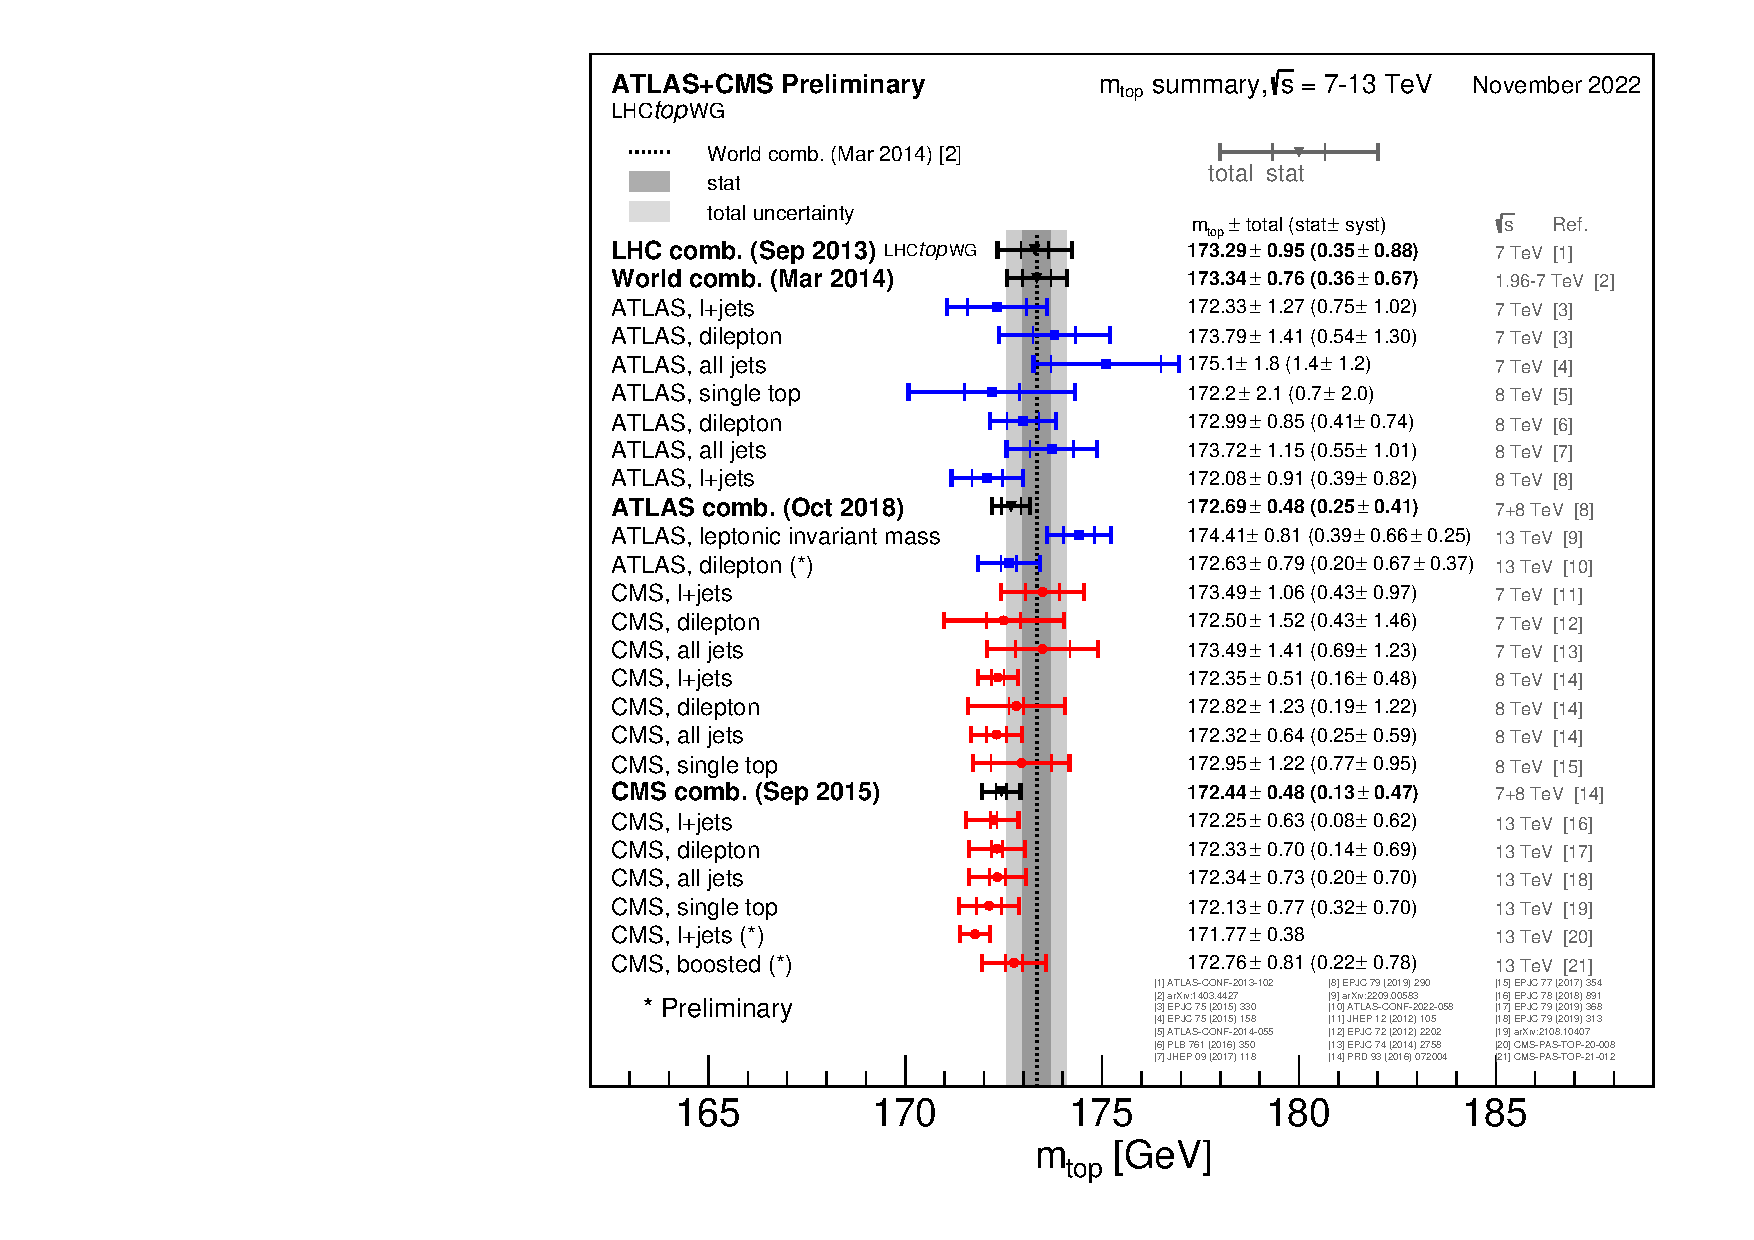
\includegraphics[width = 0.8\textwidth]{Chapter1/LHC_topMCmass_Nov22}
   	 \caption{Summary of the ATLAS and CMS $\mtop^{MC}$ measurements from top-quark decay. 
	 Results compared to Large Hadron (LHC) \mtop combination~\cite{ATLAS:2022lsz}. 
	 The most precisely studied property of the top quark is its mass.}
    	\label{fig:Chap1:top:mtop_MC}
	\end{figure}

	
       \item Indirect measurements~\cite{Amoroso:2746800}:
	The $\mtop^{\text{pole}}$ is measured from measurements of the cross-section. These methods
	rely on the dependence on the value of the $\mtop$ for the total or differential production 
	cross-sections for processes involving top quarks. Figure~\ref{fig:Chap1:top:mtop_Pole}
	presents $\mtop^{\text{pole}}$ indirect measurements.
	%$\rightarrow$ $m_{t}^{\text{pole}}$ with $O(1$~GeV$)$ precision
	\begin{figure}
    	\centering
    	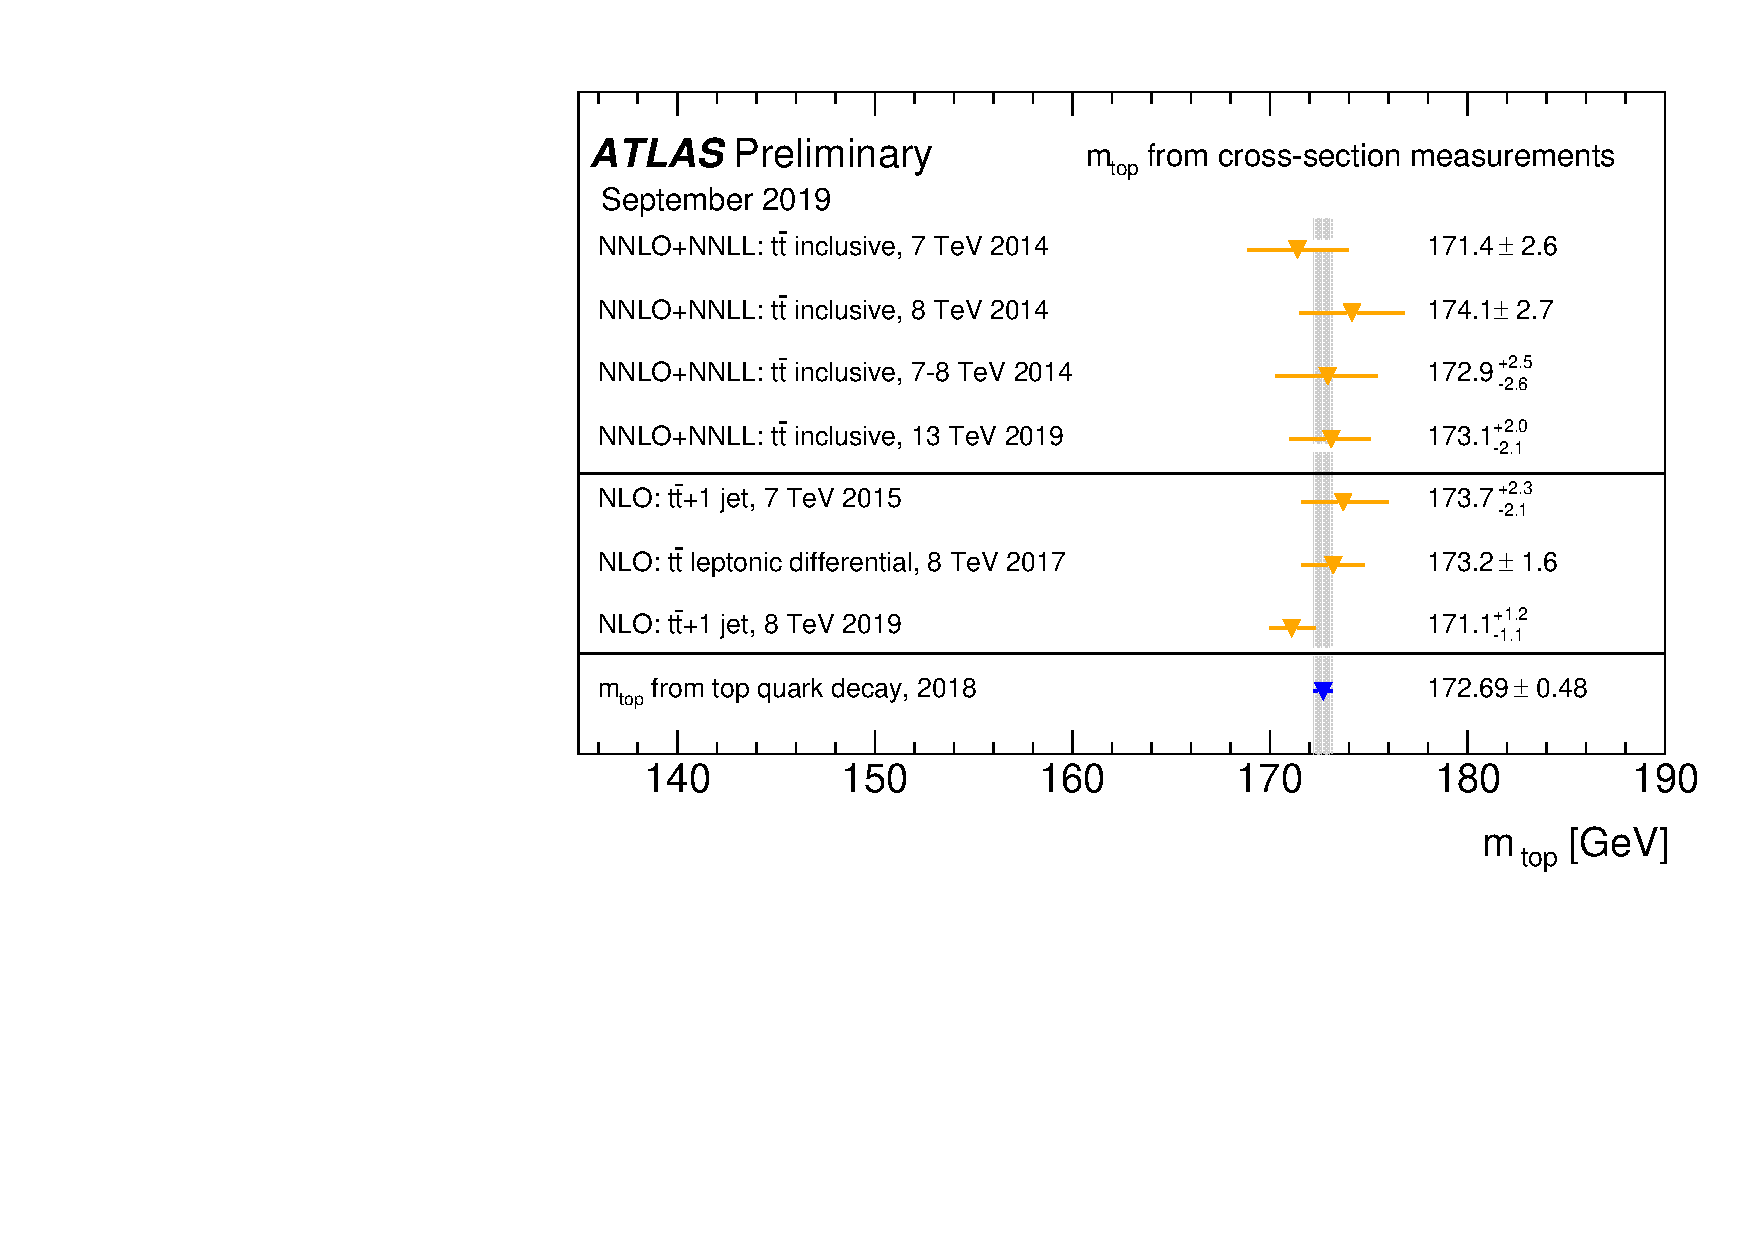
\includegraphics[width = 0.8\textwidth]{Chapter1/LHC_topPOLEmass_Sept19}
    	\caption{Summary of the measurements of the $\mtop^{\text{pole}}$ from \ttbar cross-section measurements.
    	A caparison to the measurements from top-quark decay is provided~\cite{ATLAS:2018fwq}.}
    	\label{fig:Chap1:top:mtop_Pole}
	\end{figure}
	\end{itemize} 	
	% ref:  	Strategy for ATLAS top quark mass measurements: 2021-2023
	%         	https://cds.cern.ch/record/2746800?


\pablo{No he explicado qué es  $\mtop^{MC}$ y  $\mtop^{\text{pole}}$. No hace falta, no?}
% La pole mass es la que sale en teoría
% La MC mass se mide de los hadrones que salen del top quark y no se entiende muy bien qué significa

\end{comment}

Among the properties of the top quark, its mass is the one that has received the most attention so far.
Accurate measurements of \mtop are vital for determining the parameters of the EW global fits, which are essential for evaluating the internal consistency of the SM and exploring its potential extensions\cite{ALEPH:2010aa, Baak:2014ora}. Moreover, the \mtop value influences the stability of the Higgs-boson potential, carrying which has cosmological implications~\cite{Degrassi:2012ry, Bezrukov:2007ep, DeSimone:2008ei}.
The most recent studies for the top-quark mass measurements result in $\mtop = 172.76 \pm 0.30$~GeV~\cite{Workman:2022ynf}. %~\cite{pdgTop}. 
This number is an average of the measurements at the Large Hadron (LHC) 
with ATLAS ($172.69 \pm 0.66$~GeV~\cite{ATLAS:2018fwq})
and CMS ($172.6 \pm 2.5$~GeV at CMS~\cite{CMS:2019fak}) 
and at Tevatron with CDF and D$\emptyset$ (combined result: $174.30 \pm 0.89$~GeV~\cite{CDF:2016vzt}).
These values are measured from the kinematics of  \ttbar events and refer to the $\mtop^{\text{pole}}$.%\footnote{In 
	 %particle physics, an event is the result of a collision.}.%\footnote{This \mtop results are sensitive to the 
%top quark mass used in the MC generator that is usually interpreted as the pole mass.}.
% top masses: https://pdglive.lbl.gov/DataBlock.action?node=Q007TP
% Direct measurements    :: $\mtop^{\text{MC}}$
% Indirect measurements :: $\mtop^{\text{pole}}$
 
%Figure~\ref{fig:Chap1:top:mtop_tt}  presents the results for \mtop measurements from \ttbar observables.

% Definition of mass: 
% Quark masses are fundamental parameters of QCD.  In QFT, the propagator of a massive fermion has a pole
% at $m_0$ called the pole mass, which also corresponds to the invariant mass calculated from
% its decay products. However, the quarks present a particular situation due to its confinement.
% Most measurements are based on the invariant mass of the top quark decay products.
% The measured top quark mass has been interpreted as the pole mass by the Particle Data Group.
%  For all other quarks, in contrast, the renormalised masses are used.

%The high mass of the top quark indicate its Yukawa coupling to the Higgs field of $\mathcal{O}(1)$.

%\begin{figure}
%    \centering
%    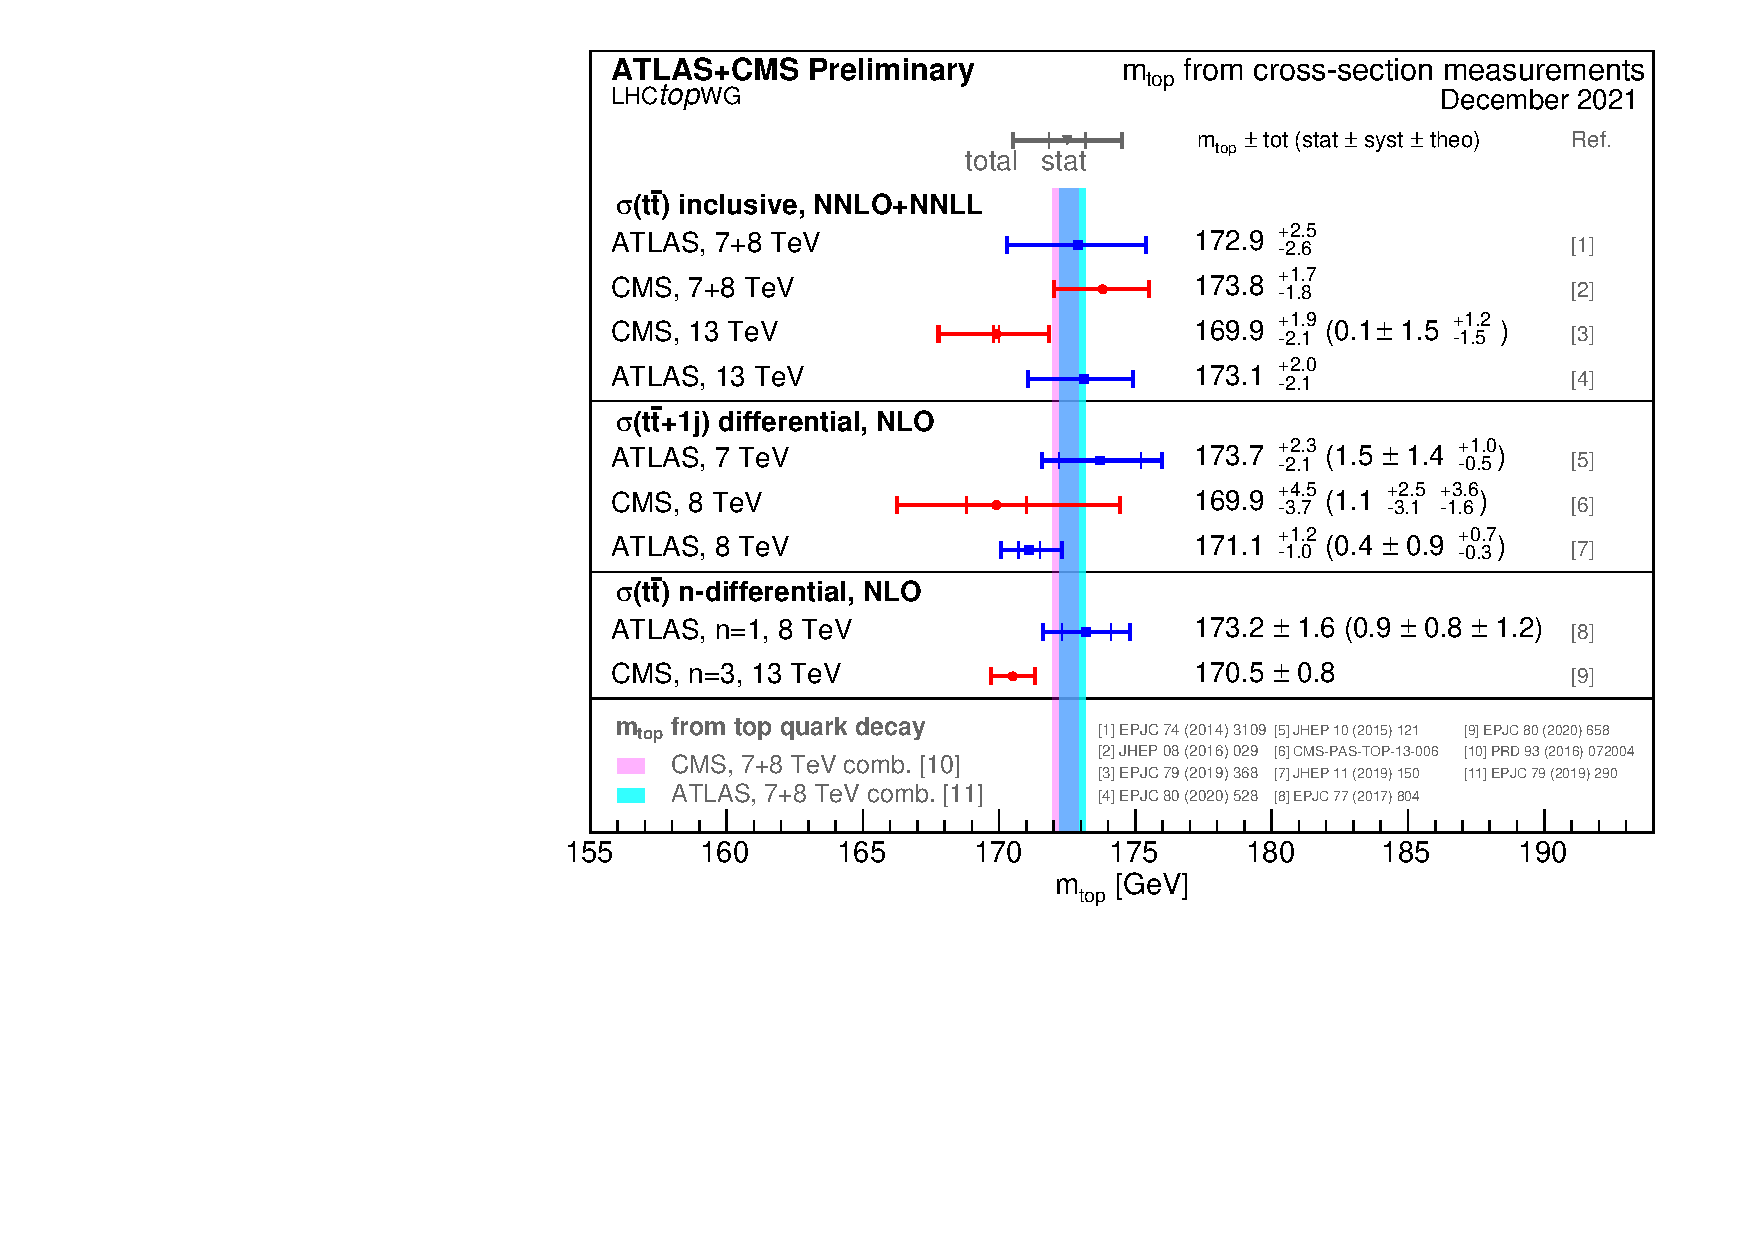
\includegraphics[width = 0.8\textwidth]{Chapter1/LHC_topmassfromXS_dec21}
%    \caption{Summary of the ATLAS and CMS measurements from \ttbar observables. 
%		Results compared to measurements from direct-top-quark decay.}
%    \label{fig:Chap1:top:mtop_tt}
%\end{figure}



% ATLAS		$\mtop = 172.69 \pm 0.25$(stat)$\pm 0.41$(syst) GeV
% CMS		$\mtop = 172.6 \pm 0.4$(stat)$\pm 1.6$(exp)$\pm 1.5$(model)  GeV
% Tevatron	$\mtop = 174.30 \pm 0.35$(stat)$\pm 0.54$(syst) GeV 




%%%%%%%%%%%%%%%%%%%%%%%%%%
%                Top quark production at LHC               %
%%%%%%%%%%%%%%%%%%%%%%%%%%
\subsection{Top-quark production at LHC}
\label{sec:Chap1:Top:Production}
The LHC is sometimes referred to as a top-quark factory due to its capacity to produce such particles in large quantities. 
In this collider, at proton--proton ($\Pproton\Pproton$) collisions, the top quark is mainly produced via
two mechanisms: through the strong interaction in top-quark--antiquark pairs (\ttbar), and by means of the \Wtb 
vertex of EW interaction in single top quarks. % associated with other particles.  
 Apart from the \ttbar (see Section~\ref{sec:Chap1:Top:Production:TopPairs}) and single top quark
(see Section~\ref{sec:Chap1:Top:Production:SingleTop}) productions, the associated \ttX and \tX 
productions play a role on producing top quarks (see Section~\ref{sec:Chap1:Top:Production:ttbar_plus_X} and 
Section~\ref{sec:Chap1:Top:Production:top_plus_X}, respectively).

Since top quarks often constitute a main background in other physics analyses, 
a better understanding of the properties of this particle will directly translate into improvements 
in those studies.

%%%%%%%%%%%%%%%%
%                Top pairs               %
%%%%%%%%%%%%%%%%        %https://twiki.cern.ch/twiki/bin/view/LHCPhysics/TtbarNNLO
\subsubsection{Top-quark--antiquark pairs production}
\label{sec:Chap1:Top:Production:TopPairs}
The production of \ttbar events is the largest source of production of top quarks in hadron collisions. This
process is one of the most important at LHC because it allows us to precisely study the properties of the top quark. 
Additionally, due to the dominance of this production mode, the \ttbar production is also a major background 
in many measurements and searches for rare processes as mentioned above. 
The physics analysis carried out in this thesis is a good example, 
where the \ttbar process is the main background in
both of the analysed decay channels.

For proton--antiproton ($\Pproton \APproton$) collisions at Tevatron or $\Pproton \Pproton$ at LHC, the \ttbar production is described by
perturbative QCD.  In this approach, a hard scattering process between the two hadrons is the result 
of an interaction between the quarks and gluons that constitute these hadrons. This model is described in detail in 
Section~\ref{sec:Chap2:PhenoOfPP}.


At LHC, gluon fusion dominates with 90\% of 
the \ttbar production. It is followed by the quark--antiquark annihilation, 
which accounts for 10\% of the total \ttbar production.
%Due to its primordial importance for the physics programme of LHC
The theoretical calculations for the \ttbar 
production at $\CM=13\,\text{TeV}$ are done to an accuracy of  next-to-next-to-leading order (NNLO)
in QCD and complemented with next-to-next-to-leading logarithmic (NNLL) resummation~\cite{Czakon_2020, Czakon:2013goa}: %\cite{Czakon:2013tha}
\begin{equation*}
\sigma^{\text{pred}}_{\text{NLO+NNLL}}(\ttbar) = 833.9^{+20.5}_{-30.0}\text{(scale)}\,\pm 21.0 \text{(PDF}+\alpha_{s}) \, ^{+22.5}_{-23.2}\text{(mass)}\,\text{pb}\,. 
\end{equation*}
% ref: https://twiki.cern.ch/twiki/bin/view/LHCPhysics/TtbarNNLO
%\pablo{(En el paper de Czakon te pone la $\sigma^{pred}_{\ttbar}$ a 14 GeV y luego un plot de $\sigma^{pred}_{\ttbar}$ vs $\CM$ pero no da numerito a 13 TeV. Tampoco hay numerito en~\cite{ATLAS:2022uqj}. El número lo saco de~\cite{ATLAS:2022qak} quien lo saca de )}
Here, PDF stands for parton distribution function and $\alpha_{s}$ is the strong coupling constant.
The scale uncertainty refers to the sensitivity to the choice of factorisation and renormalisation 
scales\footnote{In QCD and QED, the renormalisation scale is a parameter that helps 
to eliminate infinities arising in the calculations of  interactions. It is associated with the 
energy scale at which a physical process occurs.}~\cite{Czakon:2016dgf}. 
These scales are further discussed in Section~\ref{sec:Chap2:PhenoOfPP:ProtonStructure}.
The ATLAS and CMS collaborations have measured its cross-section through different final state channels and 
the most precise result obtained so far at $\sqrt{s}=13$~TeV is~\cite{ATLAS:2023gsl} 
\begin{equation*}
\sigma^{\text{obs}} (\ttbar) = 829 \pm 1\text{(stat.)}\,\pm 13\text{(syst.)}\,\pm 8\text{(lumi.)}\, \text{pb} \, .
\end{equation*}
Thanks to this large cross-section, the statistical uncertainty is not constraining the measurements of
the \ttbar production, which is performed with good precision ($\mathcal{O}(2\%)$).
This large cross-section also makes \ttbar the most relevant background in this analysis.
%Figure~\ref{fig:Chap1:top:topPairs:CrossSection} 
%its most
%recent result are, respectively, $\sigma_{\ttbar} = 836 $$\pm$$ 29$~pb~\cite{ATLAS:2022qak} and $\sigma_{\ttbar} = 791 $$\pm$$ 36$~pb~\cite{CMS:2021vhb}. 
%shows the measurements for the \ttbar production cross-section ($\sigma_{\ttbar}$) at
%\CM =$13$~TeV.
%The measurements and the theory calculations are quoted at $\mtop=172.5$~GeV.
% At Tevatron, gluon fusion was not so important, as they had proton-antiproton collisions. 


%\begin{comment}
%\begin{figure}
%\begin{minipage}[c]{0.74\linewidth}
%\subfloat[\label{fig:Chap1:top:topPairs:FeynmanB1}]
%  {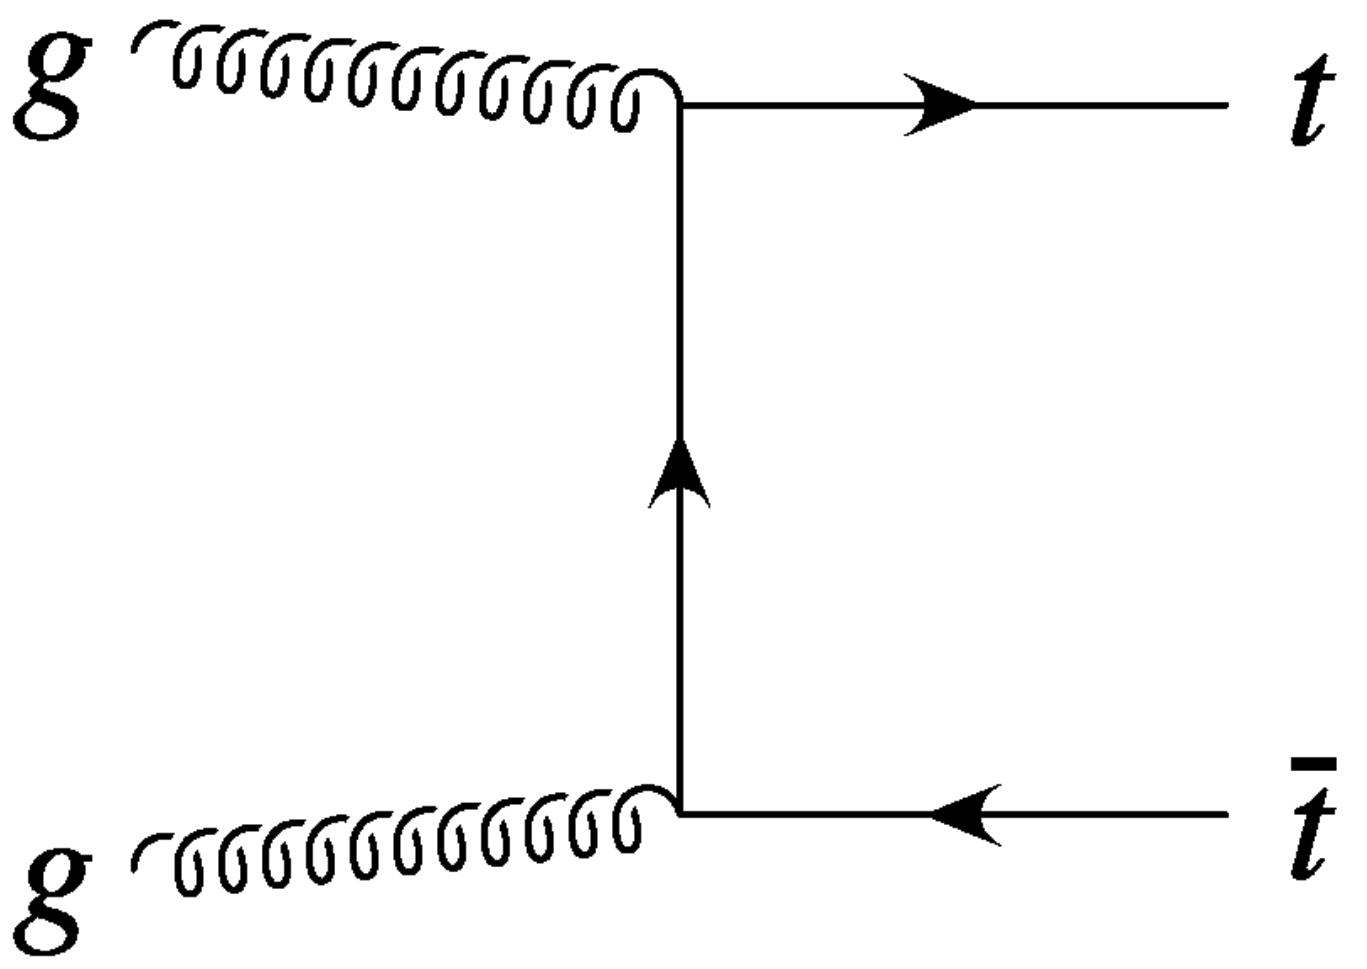
\includegraphics[width=.3\linewidth]{Chapter1/TopQuarkPairsFeynman-B1}}\hfill
%\subfloat[\label{fig:Chap1:top:topPairs:FeynmanB2}]
%  {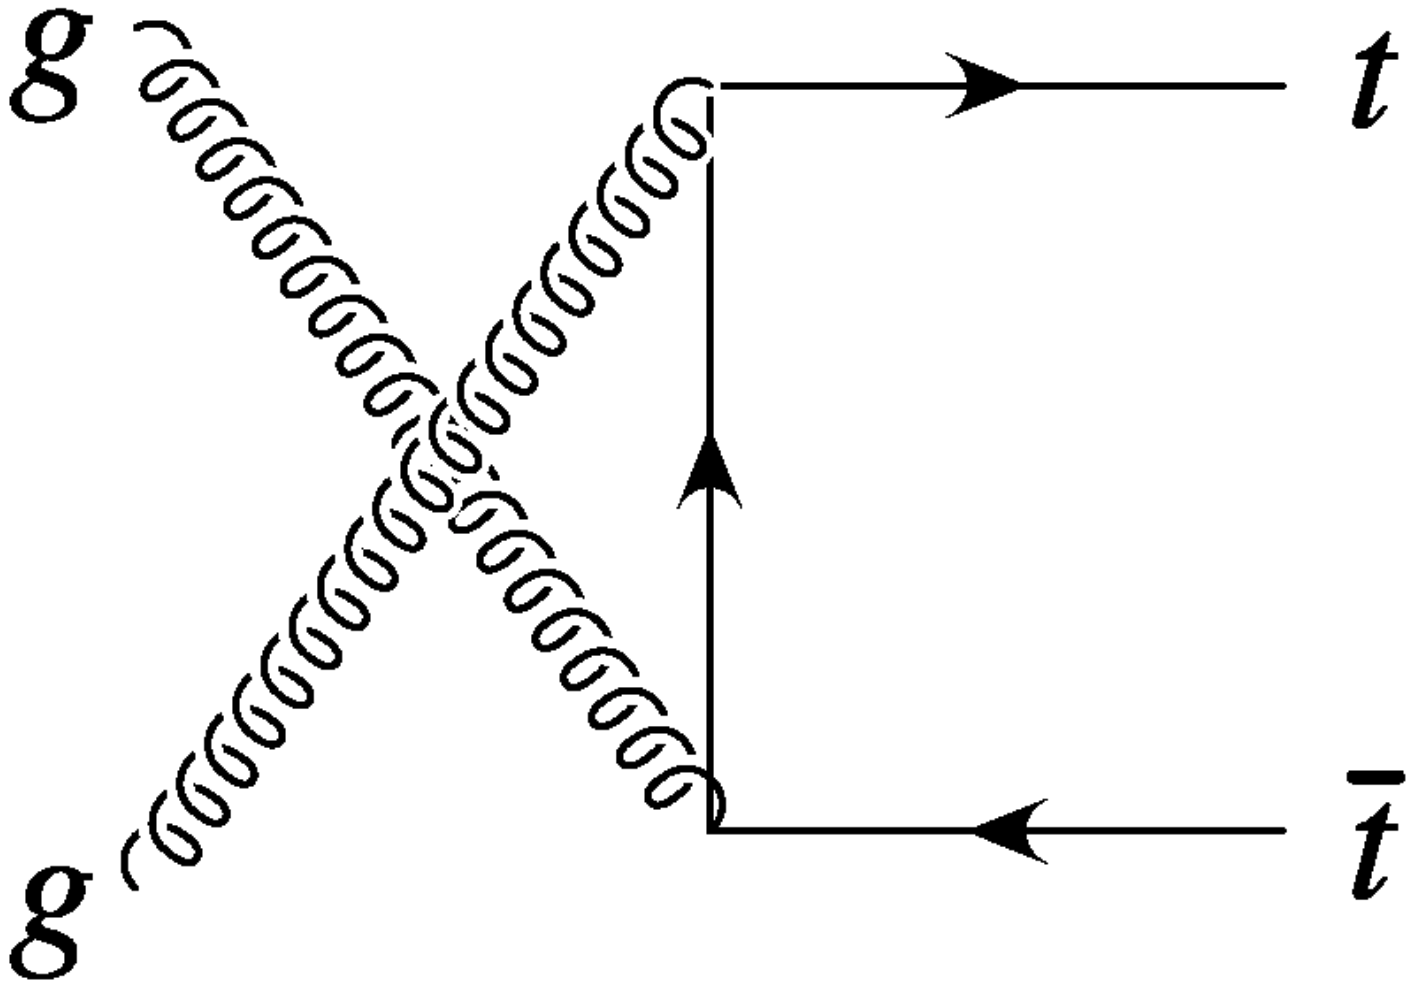
\includegraphics[width=.3\linewidth]{Chapter1/TopQuarkPairsFeynman-B2}}\hfill
%\subfloat[\label{fig:Chap1:top:topPairs:FeynmanB3}]
%  {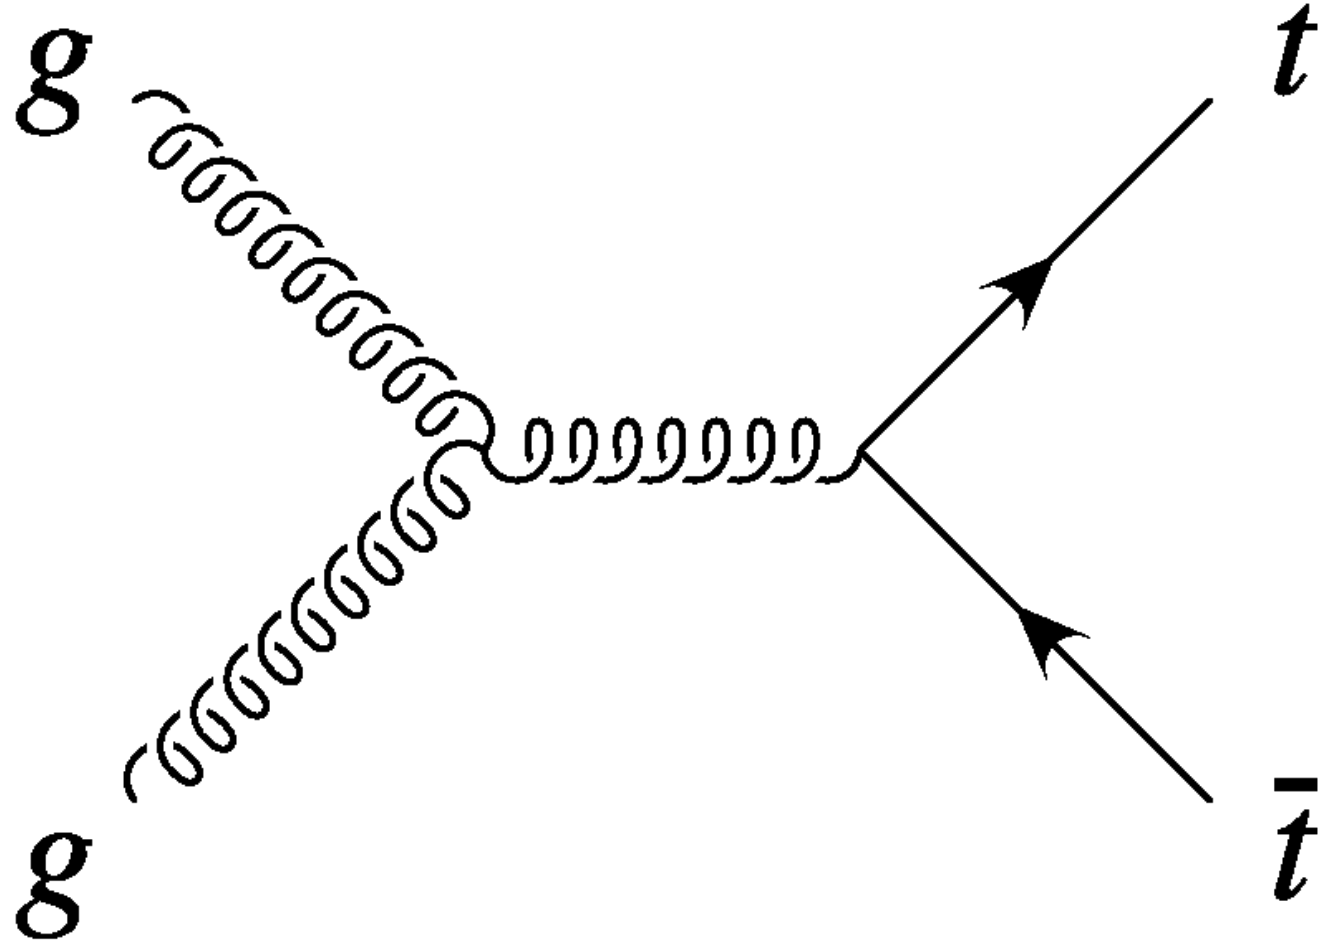
\includegraphics[width=.3\linewidth]{Chapter1/TopQuarkPairsFeynman-B3}}\hfill
%\caption{Representative Feynman diagrams of the LO processes contributing to the \ttbar 
%	production through gluon fusion at LHC.}
%\label{fig:Chap1:top:topPairs:FeynmanB}
%\end{minipage}
%\hfill
%\begin{minipage}[c]{0.25\linewidth}
%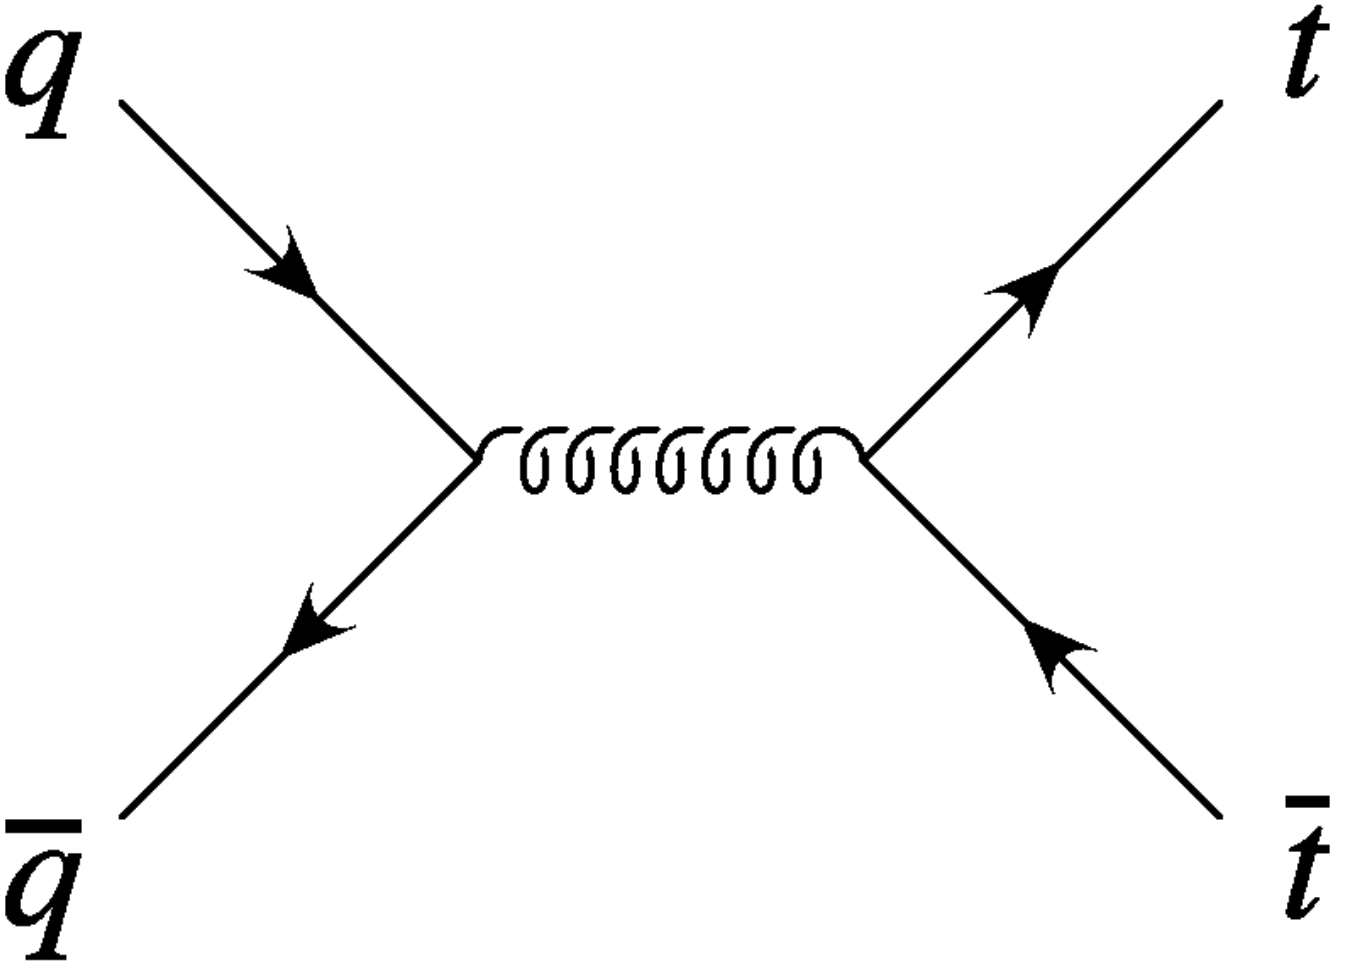
\includegraphics[width = 0.99\textwidth]{Chapter1/TopQuarkPairsFeynman-A}
%    \caption{LO Feynman diagram for \ttbar production 
%    		via quark and anti-quark annihilation.}
%    \label{fig:Chap1:top:topPairs:FeynmanA}
%\end{minipage}%
%\end{figure}
%\end{comment}

\begin{comment}
\begin{figure}
\begin{subfigure}[h]{0.23\linewidth}
	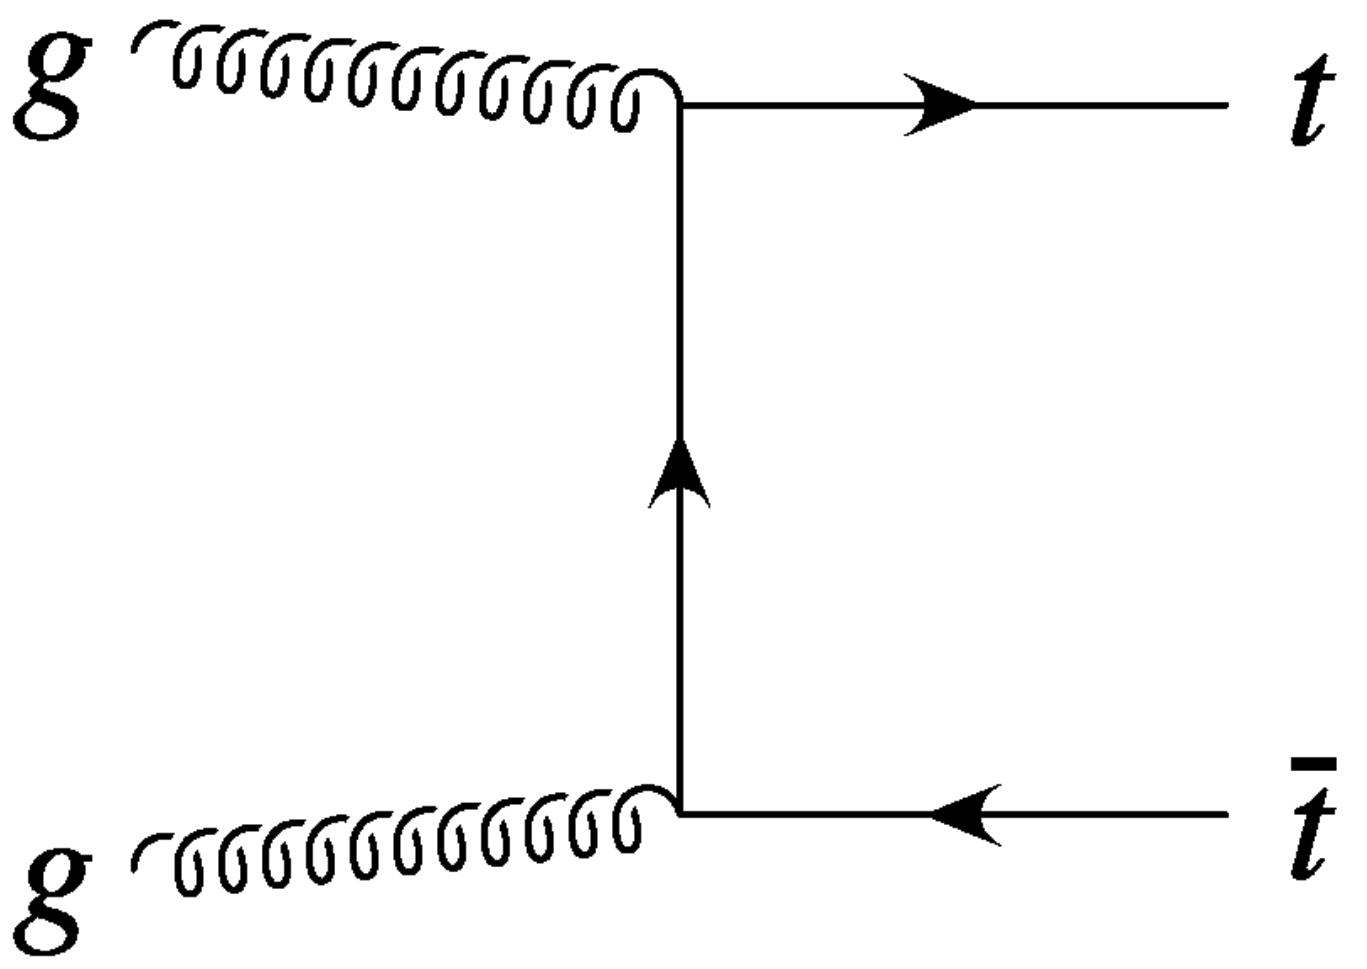
\includegraphics[width=\linewidth]{Chapter1/TopQuarkPairsFeynman-B1}
	\caption{}
	\label{fig:Chap1:top:topPairs:FeynmanB1}
\end{subfigure}
\hfill
\begin{subfigure}[h]{0.23\linewidth}
	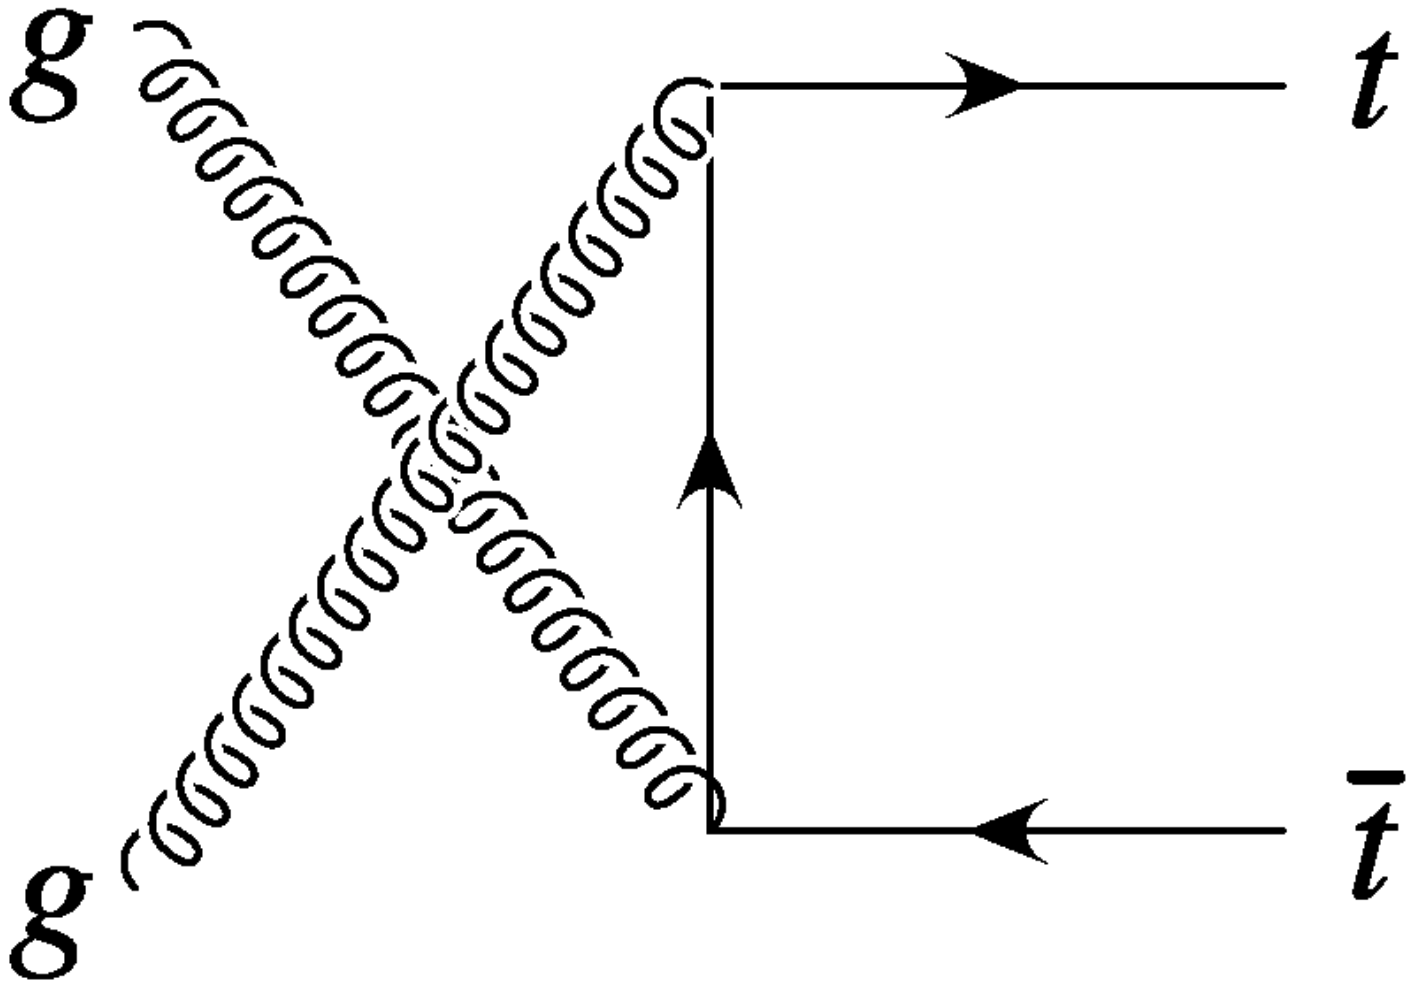
\includegraphics[width=\linewidth]{Chapter1/TopQuarkPairsFeynman-B2}
	\caption{}
	\label{fig:Chap1:top:topPairs:FeynmanB2}
\end{subfigure}
\hfill
\begin{subfigure}[h]{0.23\linewidth}
	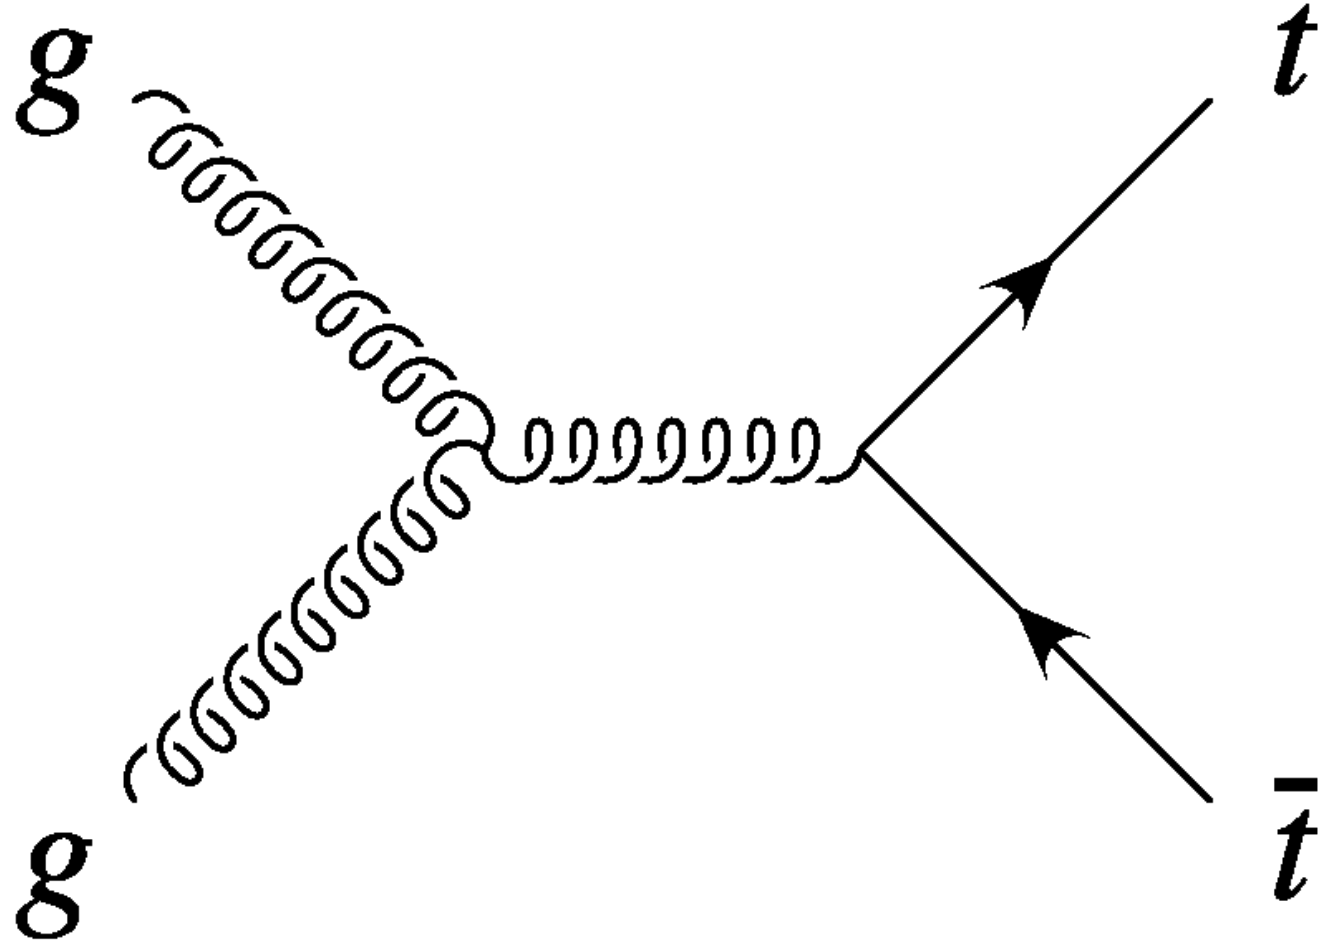
\includegraphics[width=\linewidth]{Chapter1/TopQuarkPairsFeynman-B3}
	\caption{}
	\label{fig:Chap1:top:topPairs:FeynmanB3}
\end{subfigure}
\hfill
\begin{subfigure}[h]{0.25\linewidth}
	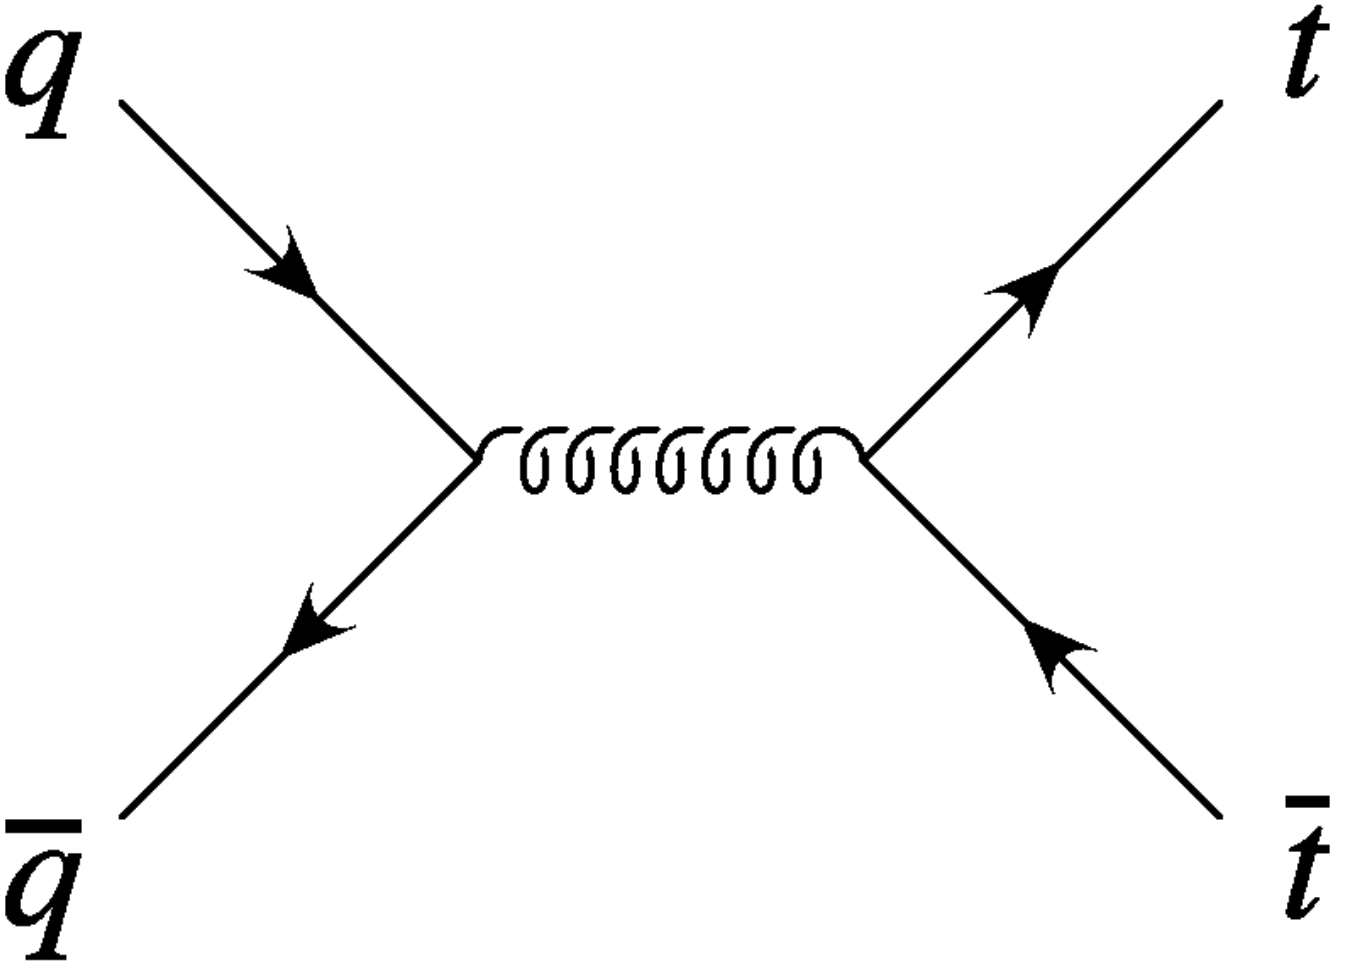
\includegraphics[width=\linewidth]{Chapter1/TopQuarkPairsFeynman-A}
	\caption{}
	\label{fig:Chap1:top:topPairs:FeynmanA}
\end{subfigure}%
\caption{Representative Feynman diagrams of the LO processes contributing to the \ttbar 
production. Where (a), (b) and (c) correspond to the production through gluon fusion 
and (d) to the production via quark--antiquark annihilation.}
\label{fig:Chap1:top:topPairs:Feynman}
\end{figure}
\end{comment}



%\begin{figure}
%\subfloat[\label{fig:Chap1:top:topPairs:FeynmanB1}]
%  {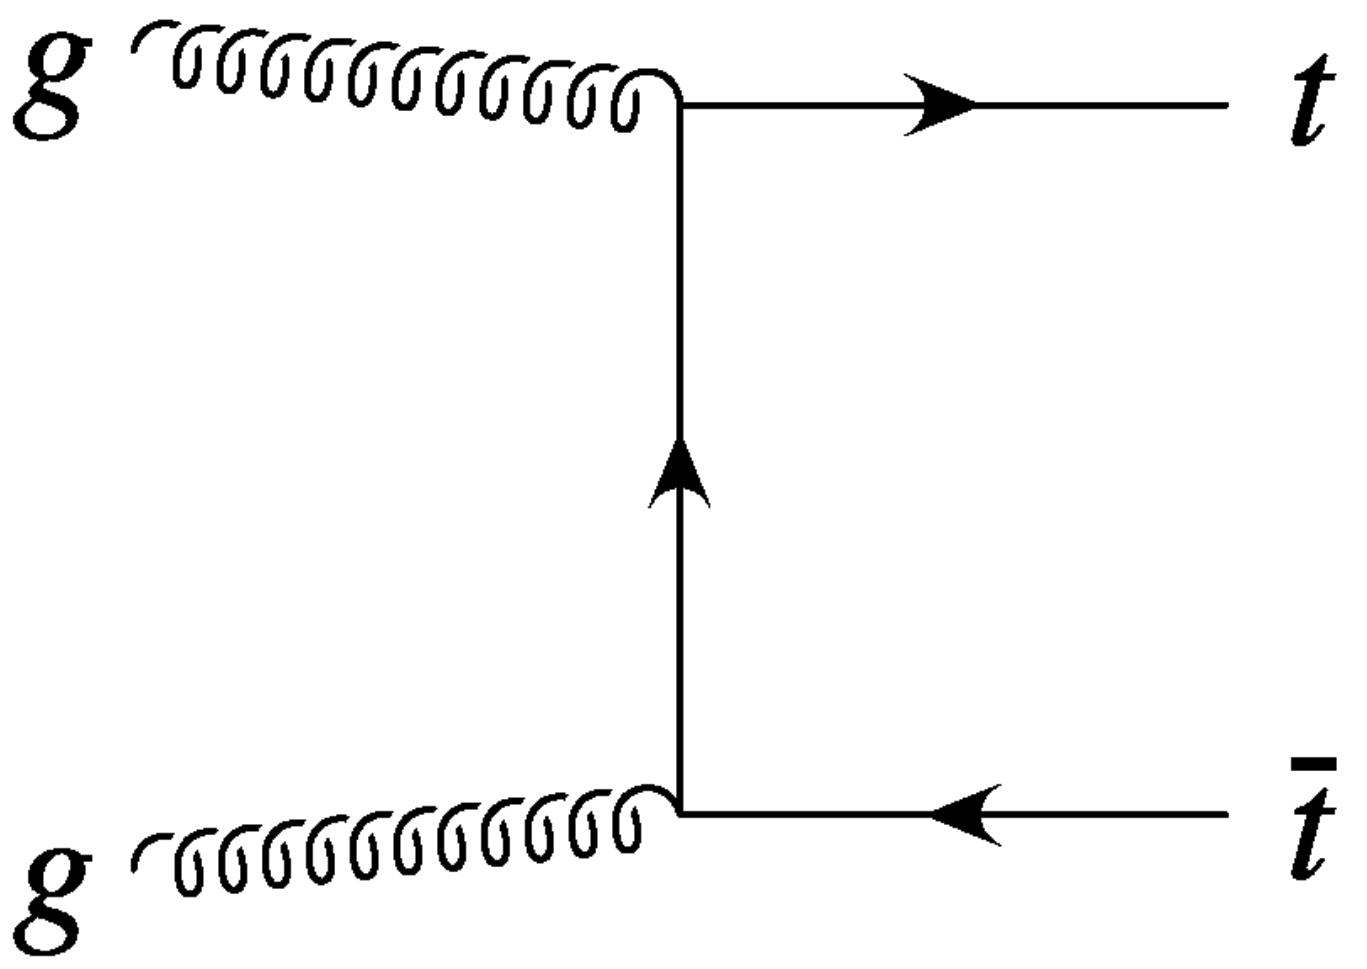
\includegraphics[width=.3\linewidth]{Chapter1/TopQuarkPairsFeynman-B1}}\hfill
%\subfloat[\label{fig:Chap1:top:topPairs:FeynmanB2}]
%  {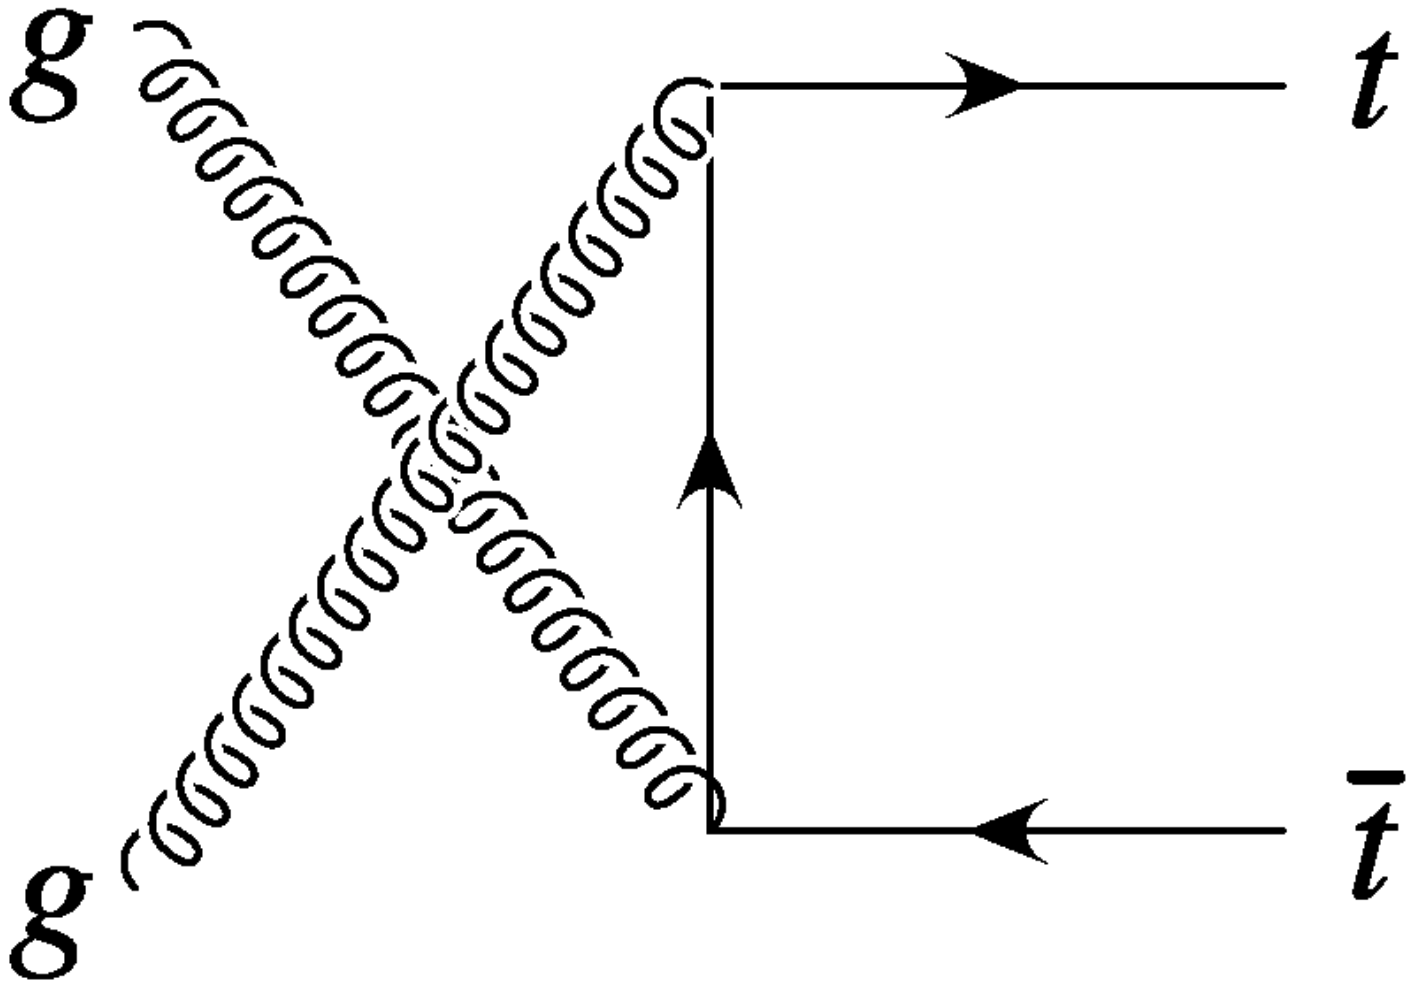
\includegraphics[width=.3\linewidth]{Chapter1/TopQuarkPairsFeynman-B2}}\hfill
%\subfloat[\label{fig:Chap1:top:topPairs:FeynmanB3}]
%  {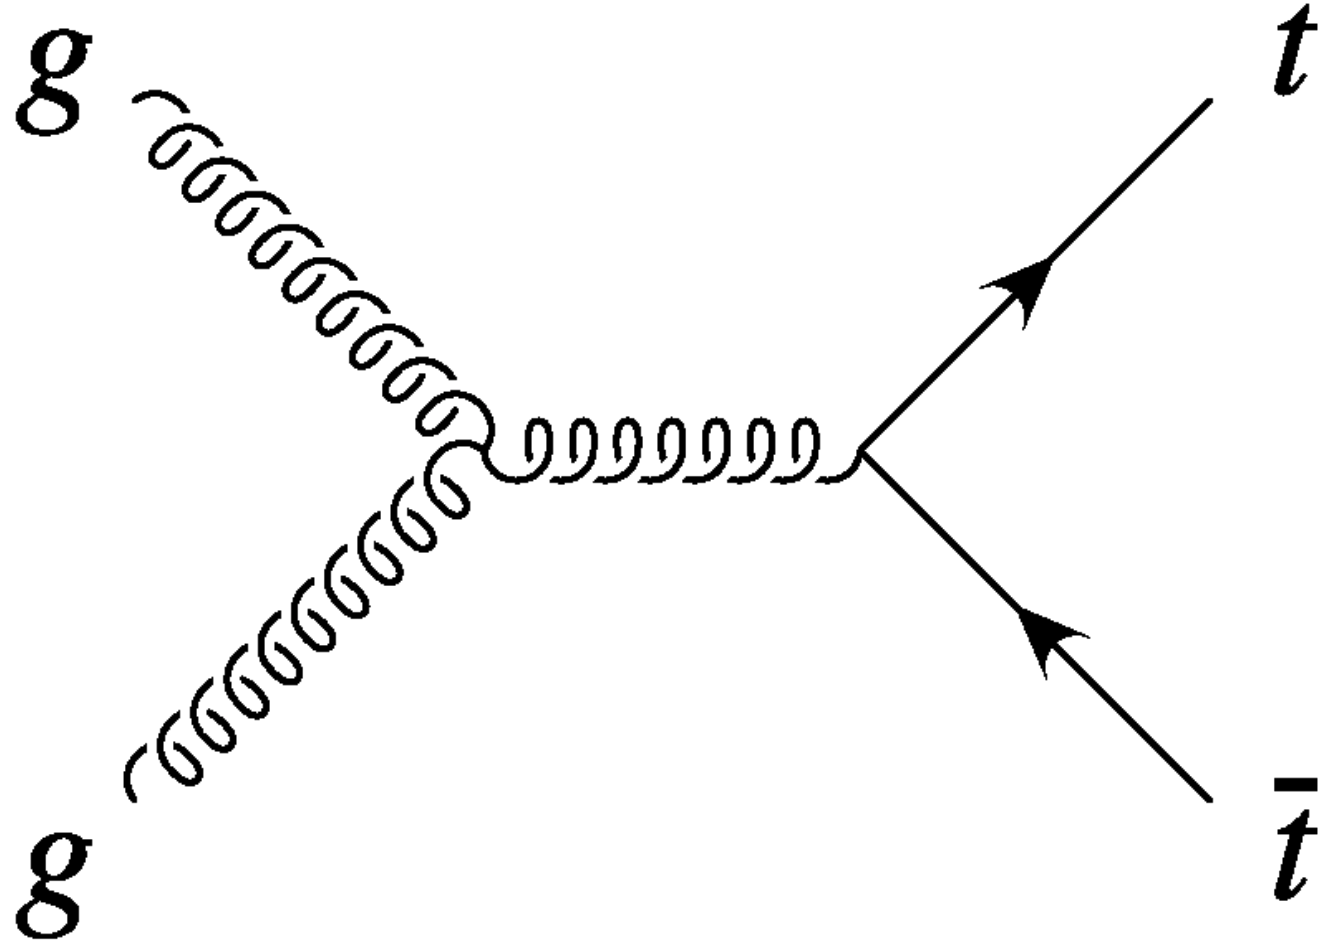
\includegraphics[width=.3\linewidth]{Chapter1/TopQuarkPairsFeynman-B3}}\hfill
%\caption{Representative Feynman diagrams of the LO processes contributing to the \ttbar production via gluon fusion at LHC.}
%\label{fig:Chap1:top:topPairs:FeynmanB}
%\end{figure}

%\begin{figure}
%    \centering
%    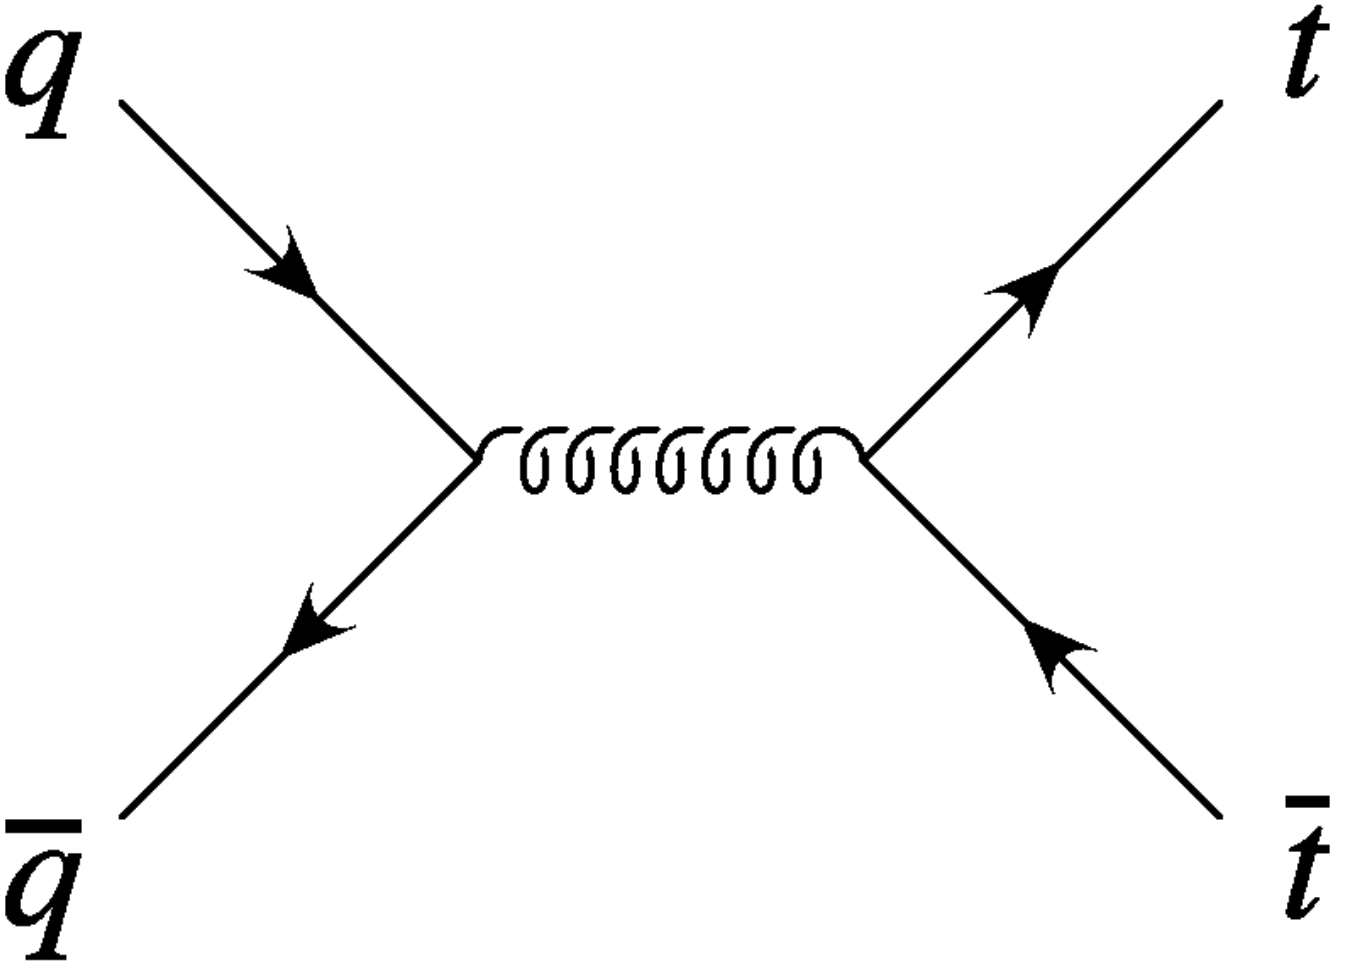
\includegraphics[width = 0.4\textwidth]{Chapter1/TopQuarkPairsFeynman-A}
%    \caption{Representative Feynman diagrams of the LO processes contributing to 
%    		the \ttbar production at LHC through quark and anti-quark annihilation.}
%    \label{fig:Chap1:top:topPairs:FeynmanA}
%\end{figure}

%\begin{figure}
%    \centering
%    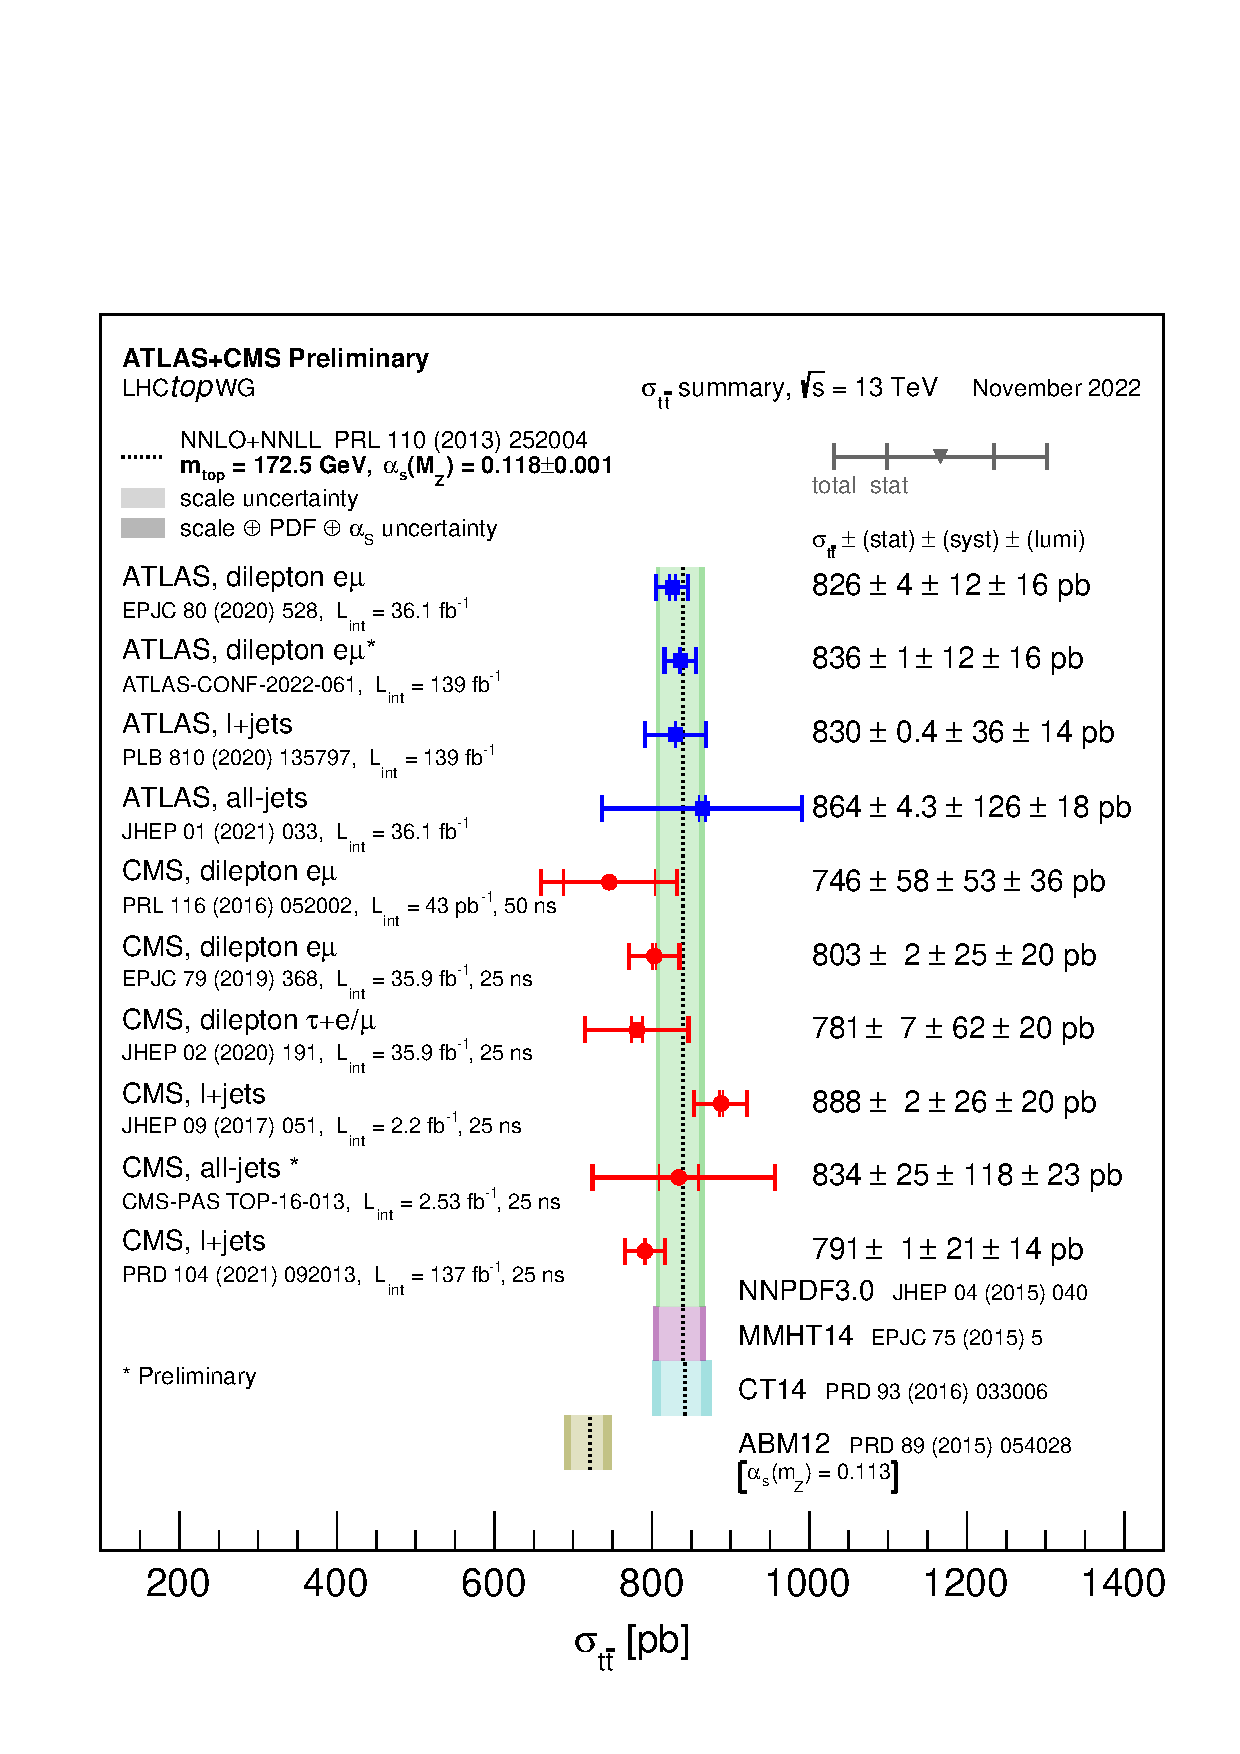
\includegraphics[width = 0.75\textwidth]{Chapter1/tt_xsec_13TeV_nov22}
%    \caption{Summary of measurements $\sigma_{\ttbar}$ at $\CM=13$~TeV compared to 
%    		the exact NNLO QCD calculation complemented with next-to-next-to-leading logarithmic resummation %\cite{ATLAS:2022uqj}. \pablo{Susana sugiere eliminar estas tablas}}
		%Update from https://twiki.cern.ch/twiki/bin/view/LHCPhysics/LHCTopWGSummaryPlots#Pair_production_cross_section
%    \label{fig:Chap1:top:topPairs:CrossSection}
%\end{figure}

%\begin{figure}
%    \centering
%    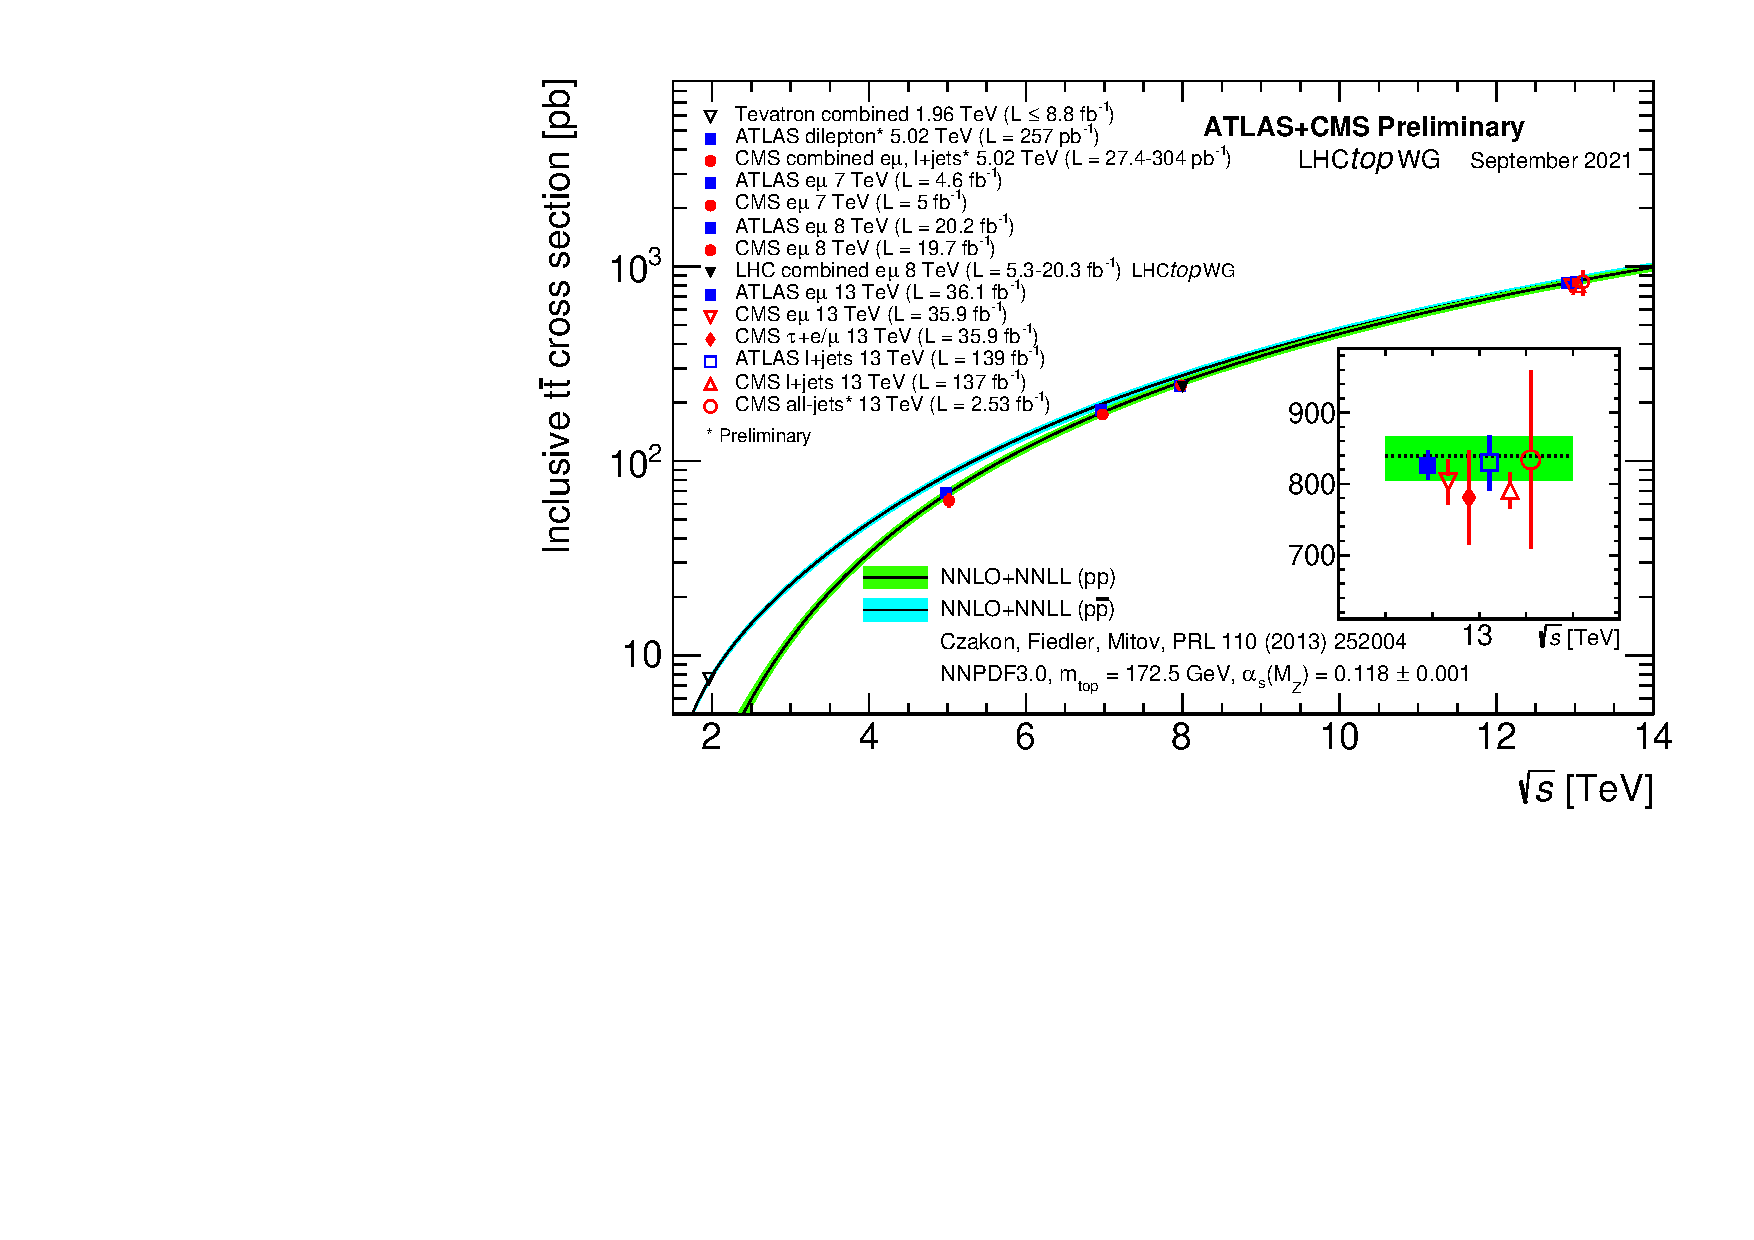
\includegraphics[width = 0.75\textwidth]{Chapter1/tt_curve_toplhcwg_sep21}
%    \caption{Summary of LHC and Tevatron measurements of the top-pair production cross-section as a function of the centre-of-mass energy}
    % The measurements and the theory calculation are quoted at mtop=172.5 GeV.
%    \label{fig:Chap1:top:topPairs:CrossSection_vs_CM}
%\end{figure}


%%%%%%%%%%%%%%%%%%%%
%                Single-top quark               %
%%%%%%%%%%%%%%%%%%%%
\subsubsection{Single-top-quark production}
\label{sec:Chap1:Top:Production:SingleTop}
In addition to the \ttbar production, the single-top-quark production is of great 
importance to the study of the top-quark properties at the LHC.  
This mechanism has a cross-section about three times smaller than that of \ttbar processes and  
it is almost exclusively produced through the EW interaction.
This is precisely the reason why single-top-quark production is essential to gather 
information about the \Wtb interaction and to directly measure the CKM
matrix element $|V_{tb}|$ at hadron colliders.
The reason why the single top quark is produced and decays via a $\Pbottom$-quark
%The reason to both decay to a $\Pbottom$-quark and be produced from a $\Pbottom$-quark 
and not via strange 
or down quarks is because the CKM elements $V_{ts}$ and $V_{td}$ 
are smaller than $V_{tb}$  by several orders of magnitude. 
%as Table~\ref{tab:Chap1:CKM} shows. %The $V_{tb}$ element not only
%determines the top production mechanism but also its decay rate.

%cross-sections for single top production: \url{https://inspirehep.net/files/9be064abc15c44ccc329d82887e6e014}
At leading order (LO), there are three production modes for 
single-top-quark events, being the \tchannel the dominant mechanism at the LHC 
with, approximately 70\% of  the single-top-quark cross-section at $\CM=13$~TeV.  % ($\sigma_{Single-\Ptop}$)
At this energy its cross-section for the \tchannel is calculated to be~\cite{Campbell:2020fhf}
\begin{equation*}
\sigma^{\text{pred}}_{\text{NLO+NNLL}} (\tchannel) = 214.2^{+2.4}_{-1.7}\text{(scale)}\,^{+3.3}_{-2.0}(\text{PDF}+\alpha_{s})\,\textrm{pb}
\end{equation*} 
and the most precise measurement is~\cite{ATLAS:2023hul}
\begin{equation*}
\sigma^{\text{obs}} (\tchannel)= 221  \pm 1 \text{(stat.)}\, \pm 13\text{(syst.)} \, \pm 2 \text{(lumi.)} \,\textrm{pb}\, .
\end{equation*} 

The other processes are the \schannel and the associated \tW production.
For the latter, the predicted cross-section is~\cite{Kidonakis:2021vob}
\begin{equation*}
\sigma^{\text{pred}}_{\text{NLO+NNLL}} (\tW) = 71.7 \pm 1.8 \text{(scale)}\, \pm 3.4\text{(PDF)}\,\textrm{pb}
\end{equation*} 
and it is measured to be~\cite{CMS:2022ytw}
\begin{equation*}
\sigma^{\text{obs}} (\tW) = 79.2 \pm 0.9 \text{(stat.)}\, \pm 7.7\text{(syst.)} \, \pm 1.2 \text{(lumi.)} \,\textrm{pb} \, .
\end{equation*} 
% source tW pred:: https://twiki.cern.ch/twiki/bin/view/LHCPhysics/SingleTopRefXsec
%source tchan and tW preds:: https://twiki.cern.ch/twiki/bin/view/LHCPhysics/SingleTopNNLORef#Single_top_quark_t_channel_cross
Only \tchannel and $\Ptop\PW$ productions are relevant to the EW 
single-top-quark production at the LHC, since the \schannel has not 
been observed at $\CM=13$~TeV. At this energy, its predicted cross-section is~\cite{Kant:2014oha}
\begin{equation*} 
	\sigma^{\text{pred}}_{\text{NLO+NNLL}} (\schannel) = 10.32^{+0.29}_{-0.24}\text{(scale)}\,\pm 0.27(\text{PDF}+\alpha_{s}) \,\textrm{pb} \, .
\end{equation*} 
%and the measured one is~\cite{TOPQ-2018-04}: %Cremonesi:2014dma
%\begin{equation*} 
%	\sigma^{\text{obs}} (\schannel) = 8.2  \pm 0.6 \text{(stat.)}\,^{+3.4}_{-2.8}\text{(syst.)} \,\textrm{pb} \, .
%\end{equation*} 
%The LO Feynman diagramas fore the three mentioned production modes are presented in Figure~\ref{fig:Chap1:top:singletop:Main}.
% \alpha_{s} = strong coupling constant    <---	This constant depends on the energy and it increases with
%									decreasing energy (asymptotic freedom). 

% Theoretical
% \sigma^{pred}_{\tchannel, \Ptop + \APtop }= 217.0^{+13.1}_{-11.1} \,\textrm{pb}$~\cite{CMS:2018lgn}

% $\sigma^{pred}_{\schannel, \Ptop + \APtop} = 10.32^{+0.56}_{-0.61} \,\textrm{pb}$ ~\cite{Kant:2014oha}

% $\sigma^{pred}_{tW, \Ptop + \APtop} = 71.7 \pm 5.2 \,\textrm{pb}$


\begin{comment}
\begin{figure}[h]
     \centering
     \begin{subfigure}[b]{0.3\textwidth}
         \centering
         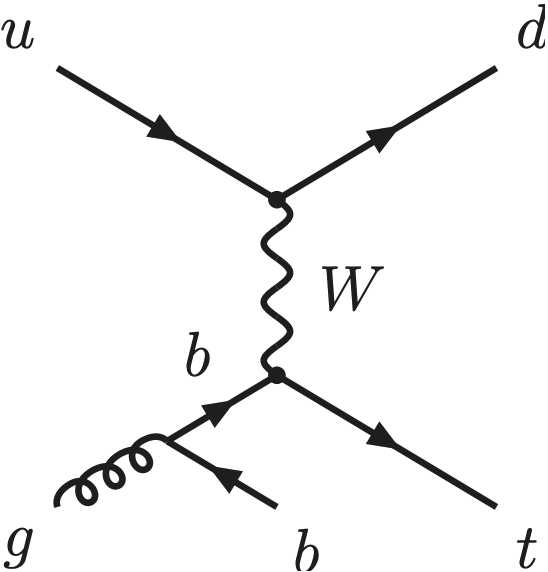
\includegraphics[width=\textwidth]{Chapter1/Single-top-tchannel-A}
         \caption{\tchannel}
         \label{fig:Chap1:top:singletop:tchannel_A}
     \end{subfigure}
     \hfill
     \begin{subfigure}[b]{0.3\textwidth}
                \centering
         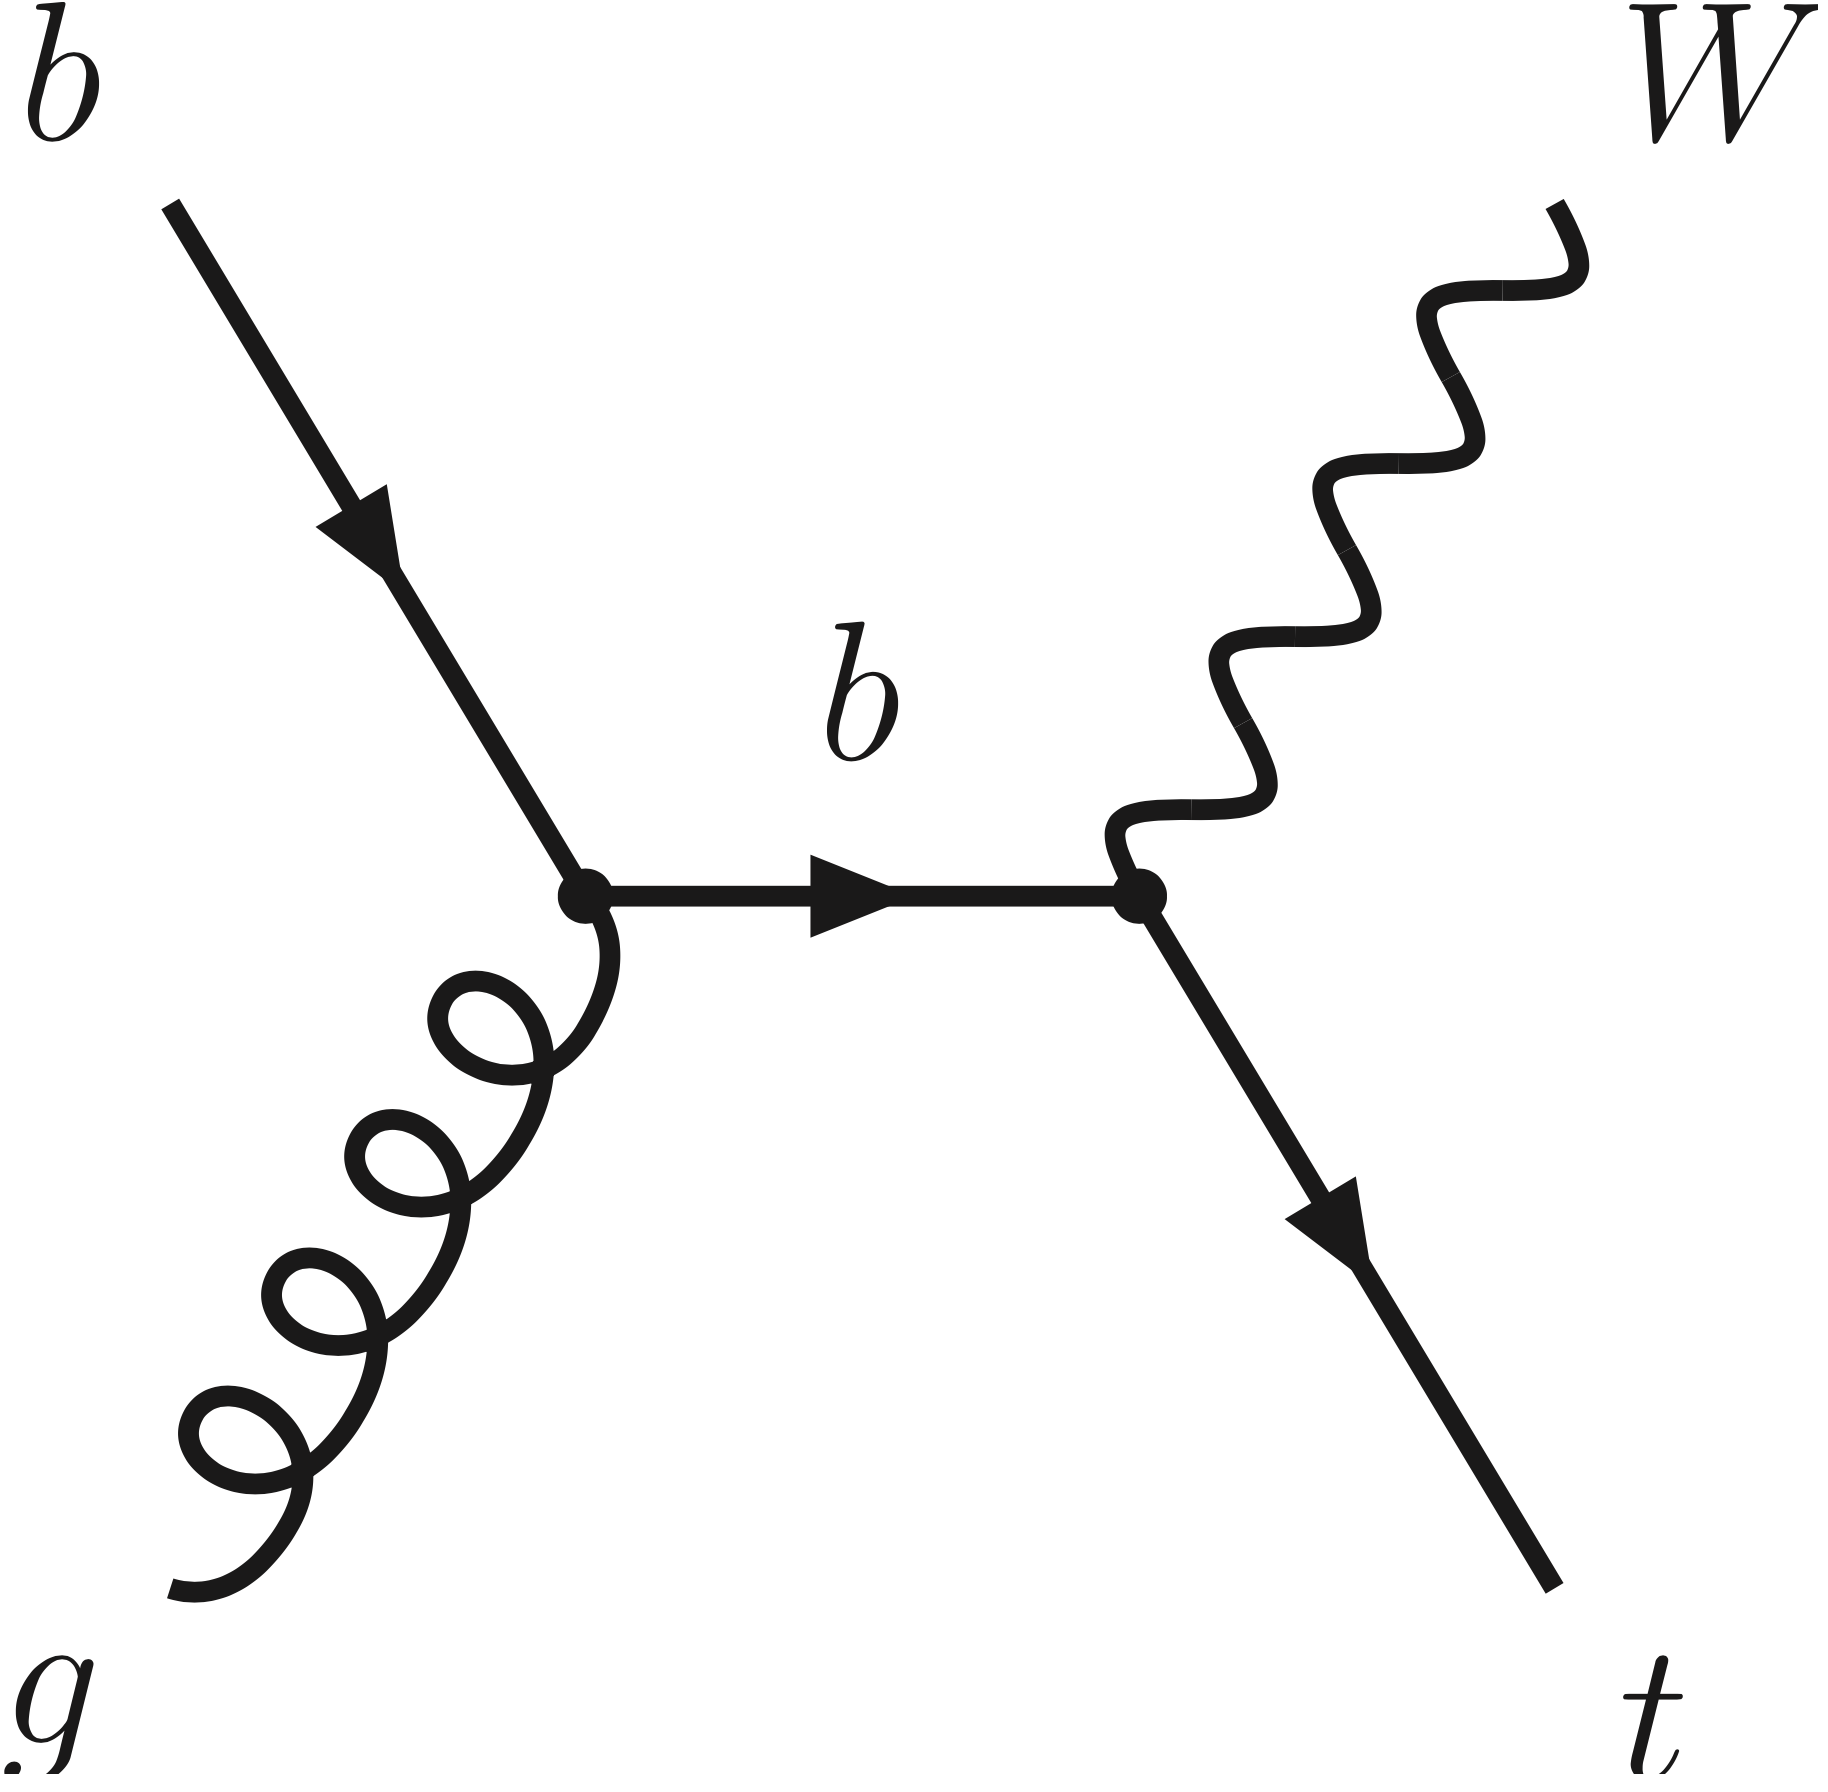
\includegraphics[width=\textwidth]{Chapter1/Single-top-Wt-B}
         \caption{\tW-channel}
         \label{fig:Chap1:top:singletop:tW_B}
     \end{subfigure}
     \hfill
     \begin{subfigure}[b]{0.3\textwidth}
         \centering
         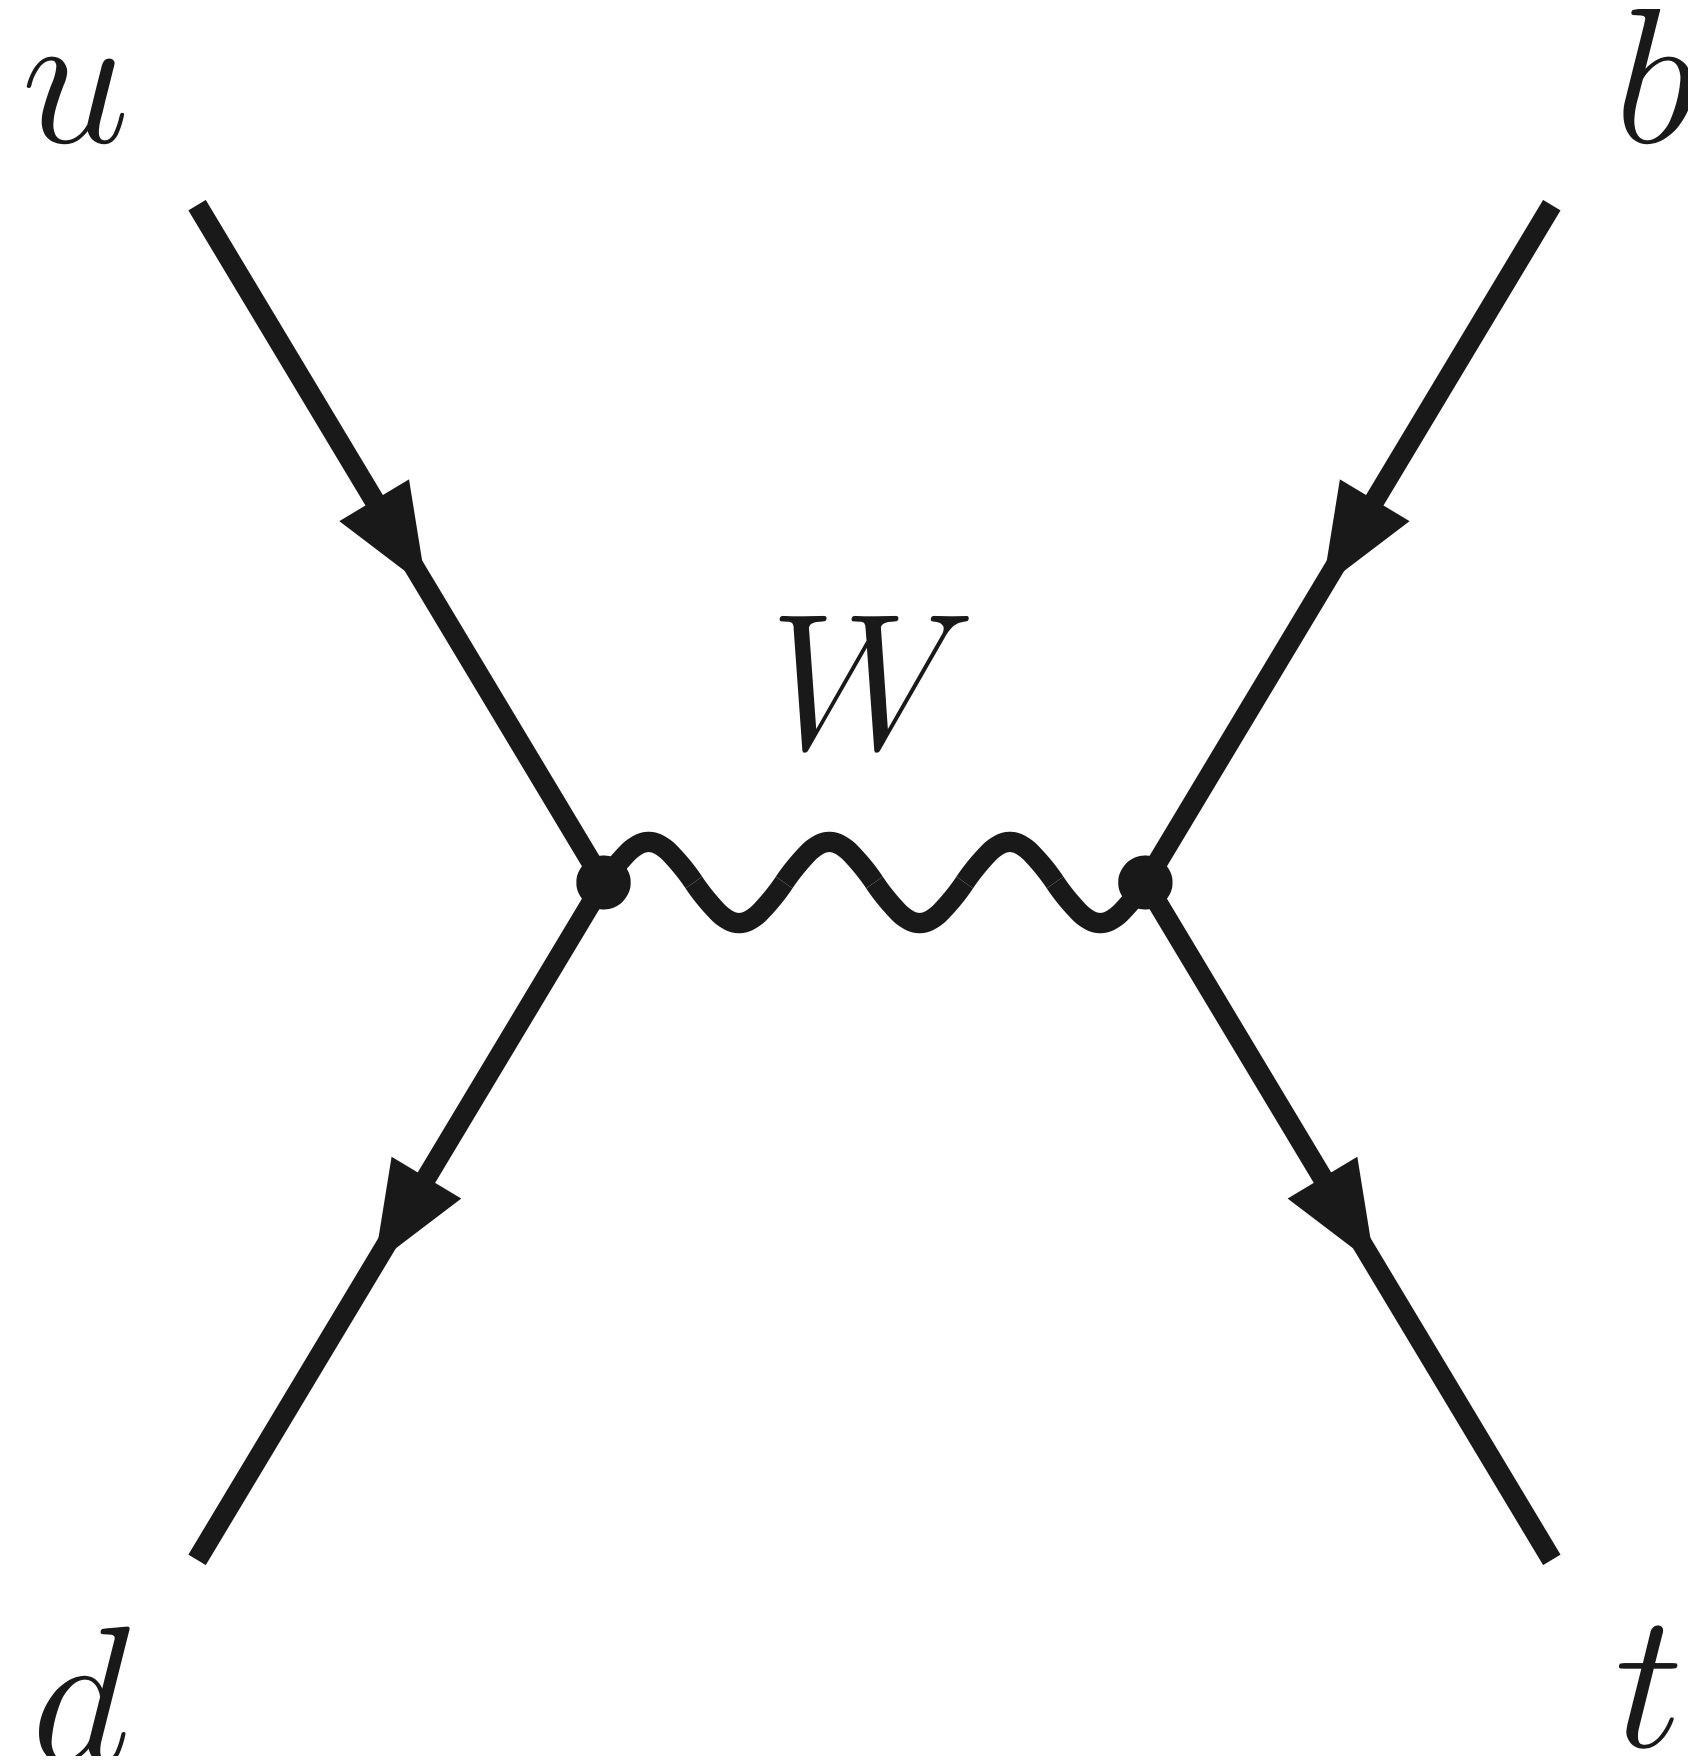
\includegraphics[width=\textwidth]{Chapter1/Single-top-schannel}
         \caption{\schannel}
         \label{fig:Chap1:top:singletop:schannel}
     \end{subfigure}
        \caption{Representative Feynman diagrams for the main three single-top-quark production channels at LO. 
        Observe that the \Pup and 
        \Pdown quarks could be substituted by \Pcharm and \Pstrange quarks.}
        \label{fig:Chap1:top:singletop:Main}
\end{figure}
\end{comment}




\begin{comment}
%%%     Single-top quark   :::  t-channel
\paragraph{\tchannel}\mbox{}\\
This production mode involves the scattering of a light quark and a gluon from the 
proton sea as shown in Figure~\ref{fig:Chap1:top:singletop:tchannel}.
Note that additional diagrams to those in Figure~\ref{fig:Chap1:top:singletop:tchannel} 
are obtained by either replacing the \Pup and \Pdown by a \Pcharm and \Pstrange
quarks or by switching the light quarks in the fermion line. The diagrams for antitop 
production are the charge conjugate of the ones presented. 

\begin{figure}
     \centering
     \begin{subfigure}[b]{0.3\textwidth}
         \centering
         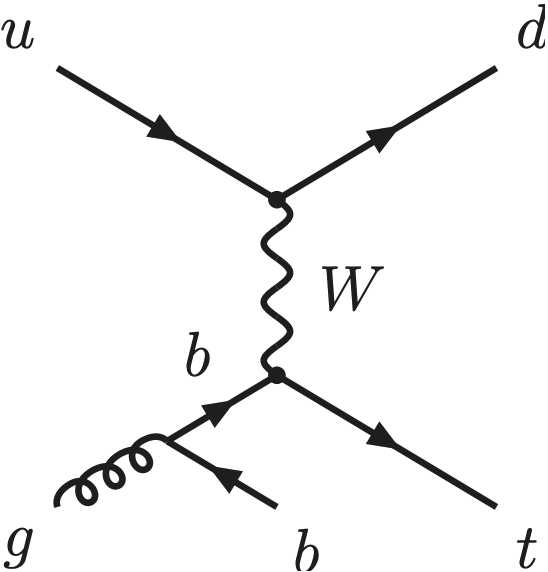
\includegraphics[width=\textwidth]{Chapter1/Single-top-tchannel-A}
         \caption{}
         \label{fig:Chap1:top:singletop:tchannel_A}
     \end{subfigure}
     \hfill
     \begin{subfigure}[b]{0.3\textwidth}
         \centering
         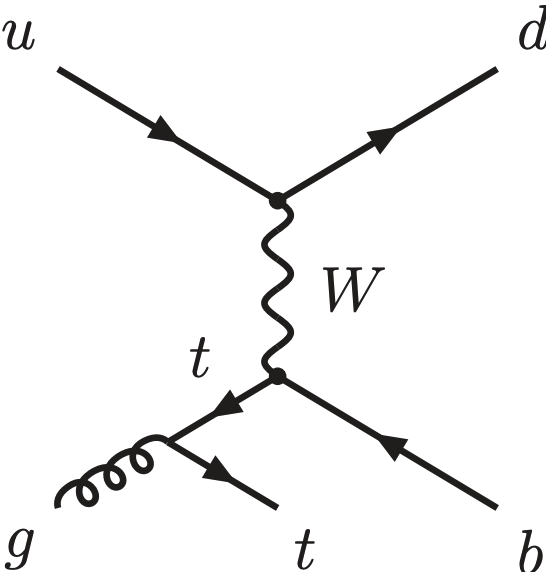
\includegraphics[width=\textwidth]{Chapter1/Single-top-tchannel-B}
         \caption{}
         \label{fig:Chap1:top:singletop:tchannel_B}
     \end{subfigure}
     \hfill
     \begin{subfigure}[b]{0.3\textwidth}
         \centering
         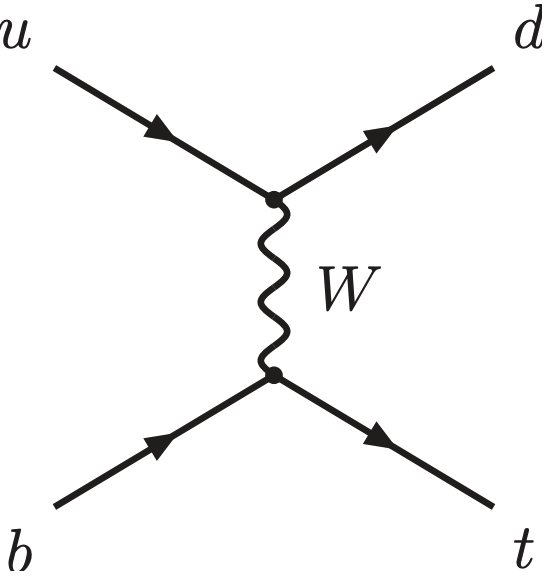
\includegraphics[width=\textwidth]{Chapter1/Single-top-tchannel-C}
         \caption{}
         \label{fig:Chap1:top:singletop:tchannel_C}
     \end{subfigure}
        \caption{Representative Feynman diagrams for the single-top-quark production in the \tchannel process. Observe that the \Pup and 
        \Pdown quarks could be substituted by \Pcharm and \Pstrange quarks.}
        \label{fig:Chap1:top:singletop:tchannel}
\end{figure}

The measurements cross-sections at $13$~TeV for single top quark ($\sigma_{\tchannel, \Ptop}$) 
and single-anti-top-qaurk ($\sigma_{\tchannel, \APtop}$) quarks in the \tchannel production are 
shown in Figure~\ref{fig:Chap1:top:singletop:tchannel_CrossSection}.
The theoretical calculation at next-to-leading order
(NLO) at $13$~TeV is $\sigma^{pred}_{\tchannel, \Ptop + \APtop }= 217.0^{+13.1}_{-11.1} \,\textrm{pb}$
\cite{CMS:2018lgn}. Due to the difference of valence quarks in the proton, the ratio 
between $\sigma^{pred}_{\tchannel, \Ptop}$ and $\sigma^{pred}_{\tchannel, \APtop}$ is 1.56. These numbers 
are obtained using \HATHOR[2.1]~\cite{Kant:2014oha, Aliev:2010zk} and a \mtop of $172.5$~GeV.
%\begin{align*}
	%\sigma_{\tchannel, \Ptop} &= 136^{+4.1}_{-2.9} (\textrm{scale}) \pm 3.5(\textrm{PDF}+\alpha_{s})\,\textrm{pb,} \\
	%\sigma_{\tchannel, \APtop} &= 81.0^{+2.5}_{-1.7} (\textrm{scale}) \pm 3.2(\textrm{PDF}+\alpha_{s})\,\textrm{pb,} \\
	%\sigma_{\tchannel, \Ptop + \APtop} &= 217^{+6.6}_{-4.6} (\textrm{scale}) \pm 6.5(\textrm{PDF}+\alpha_{s})\,\textrm{pb.}
	%\sigma_{\tchannel, \Ptop} &= 136^{+7.6}_{-6.4}\,\textrm{pb,} \\
	%\sigma_{\tchannel, \APtop} &= 81.0^{+5.7}_{-4.9} \,\textrm{pb,} \\
	%\sigma_{\tchannel, \Ptop + \APtop} &= 217.0^{+13.1}_{-11.1} \,\textrm{pb.} \\
%\end{align*} % CMS Experimental results for these cross-sections in: https://arxiv.org/pdf/1901.05247.pdf


\begin{figure}[h]
    \centering
    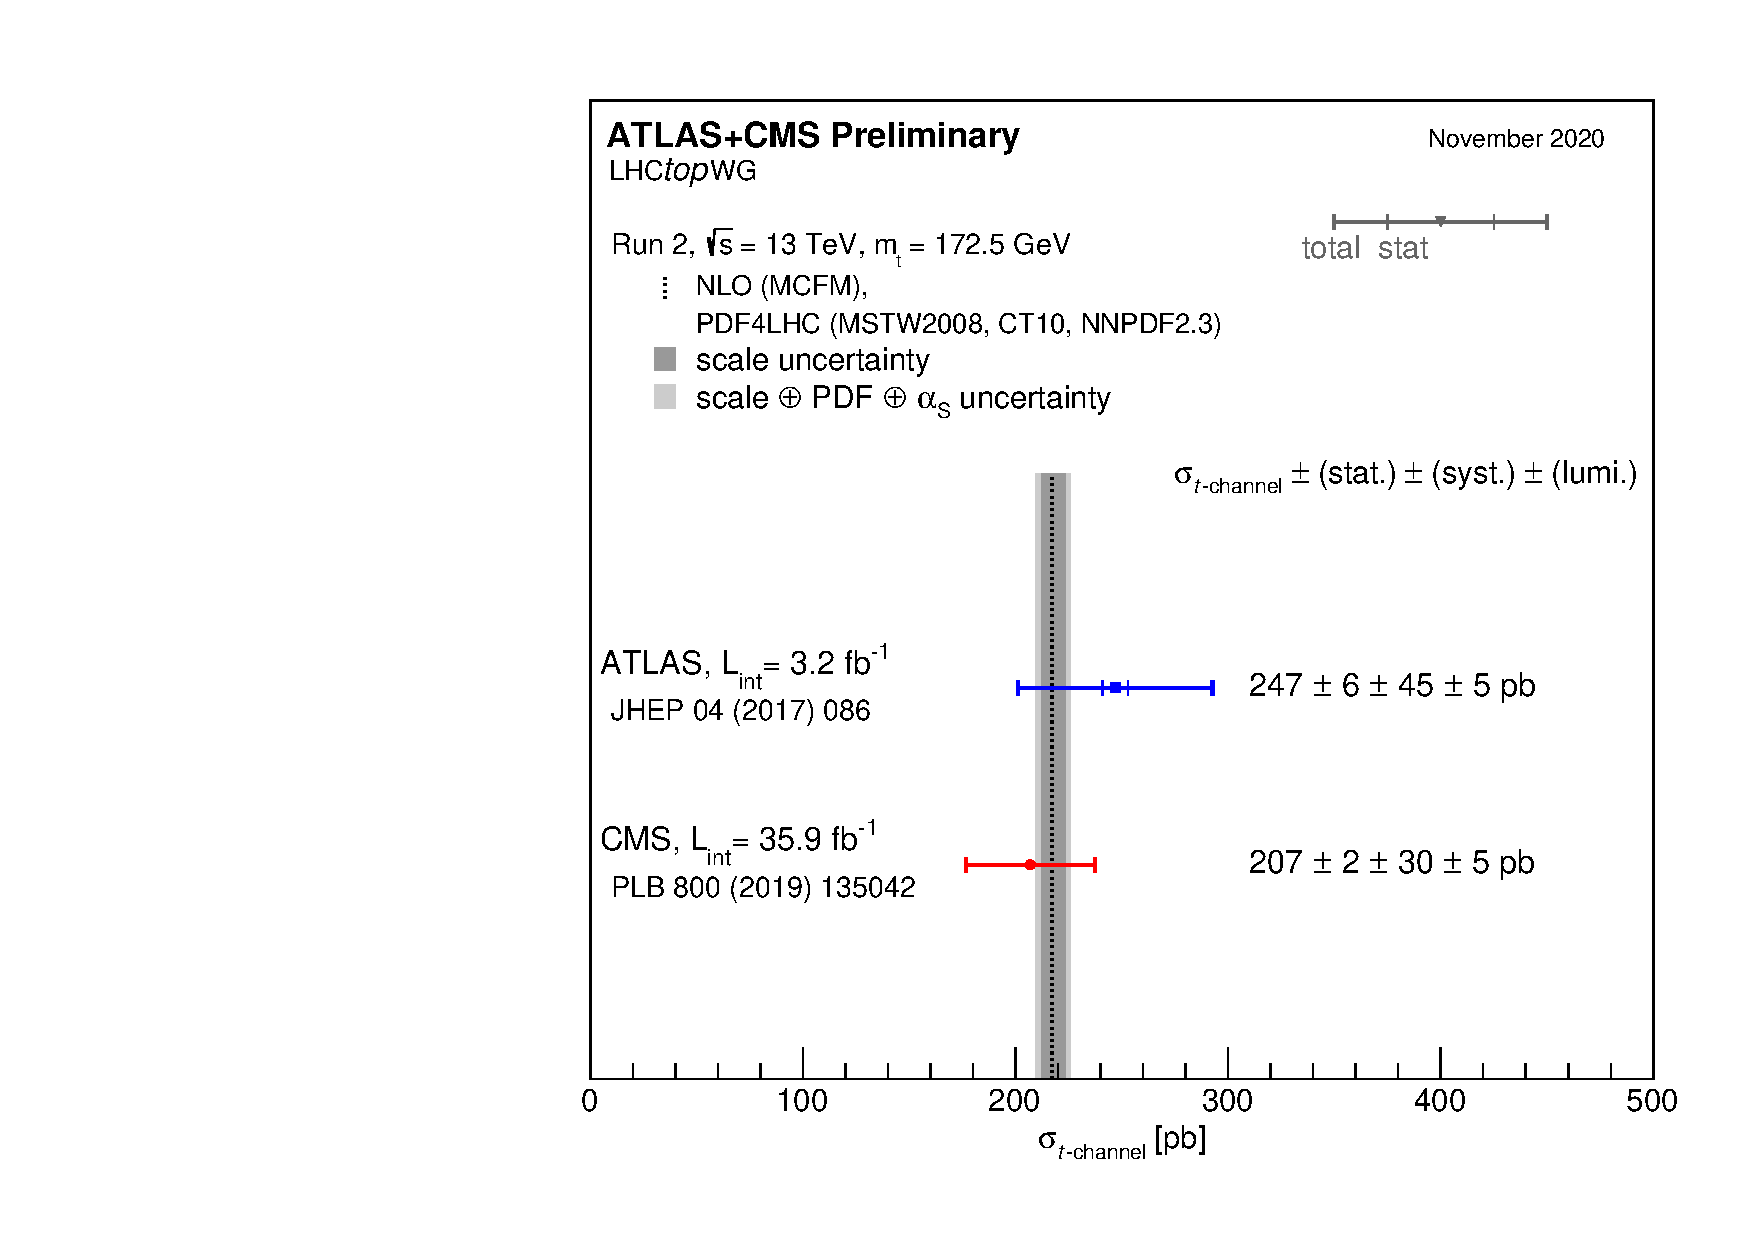
\includegraphics[width = 0.75\textwidth]{Chapter1/singletop_tchan_xsec_13_lhc_nov20}
    \caption{Summary of the ATLAS and CMS measurements of the single-top-quark production cross-sections in the \tchannel at $13$~TeV. The measurements are compared to NLO calculations~\cite{ATLAS:2022uqj}.}
    \label{fig:Chap1:top:singletop:tchannel_CrossSection}
\end{figure}


The dominant process in the SM is the one in diagram \ref{fig:Chap1:top:singletop:tchannel_A}, while 
the one in \ref{fig:Chap1:top:singletop:tchannel_B} is included in order to form a gauge invariant set 
but its contribution is not very significative since for the gluon is easier to decay to $\Pbottom\APbottom$ 
pair than to a $\Ptop\APtop$ pair. These two $2 \rightarrow 3$ production modes are known 
as 4 Flavour Scheme (FS) because the proton is considered to be composed
by four quark flavours (\Pup, \Pdown, \Pcharm and \Pstrange). It is characterised by having a \Pbottom 
quark in the final state. This final-state \Pbottom-quark is sometimes referred to as second\footnote{The 
first would be the one from the top quark decay.}.% \Pbottom and it 
%has a transverse momentum (\pT) distribution peaking around 2 or 3 GeV as can be seen 
%in Figure~\ref{fig:Chap1:top:singletop:tchannel:ptVSeta}. This is the reason why the final \Pbottom quark 
%from the gluon splitting frequently goes undetected, because it does not pass the \pT threshold of the detector. 
%This is why, at detector level, whenever only jet is identified as originated from a \Pbottom quark, it is assumed to be
%the \Pbottom from the top-quark decay. This particularity becomes more important in  Chapter \ref{chap:Analysis_tH},
%where the number of detected \btagged jets is a relevant variable for the definition of the preselection region.


The $2 \rightarrow 2$ process in \ref{fig:Chap1:top:singletop:tchannel_C} is known as 
5FS because the proton has 
four flavours of quarks and since the process has a \Pbottom quark in the initial state, there are the five flavours.
The simulations for the 4FS and 5FS diagrams are produced separately and
merged afterwards. When adding the two contributions, some double-counting may appear due to the overlap in the phase space so one has to be careful. The naming 4FS and 5FS is later used again for the associated \tH production.


%%%     Single-top quark   :::  s-channel
\paragraph{\schannel}\mbox{}\\
The \schannel process is the one with less impact among single-top-quark production channels.  
It is depicted in Figure~\ref{fig:Chap1:top:singletop:schannel}. 
This production mode is also referred to as the quark-antiquark annihilation or $W^{*}$ process  and it is very similar
to the Drell-Yann. 

According to the LHC cross-section group, at $\CM=13$~TeV, the combined 
cross-section for the single top and single anti-top production in the \schannel 
is $\sigma^{pred}_{\schannel, \Ptop + \APtop} = 10.32^{+0.56}_{-0.61} \,\textrm{pb}$ 
\cite{Kant:2014oha}.
%\begin{align*}
%	\sigma_{\schannel, \Ptop} &= 6.35^{+0.18}_{-0.15} (\textrm{scale}) \pm 0.9(\textrm{PDF}+\alpha_{s})\,\textrm{pb,} \\
%	\sigma_{\schannel, \APtop} &= 3.97^{+0.11}_{-0.09} (\textrm{scale}) \pm 0.15(\textrm{PDF}+\alpha_{s})\,\textrm{pb,} \\
%	\sigma_{\schannel, \Ptop + \APtop} &= 10.32^{+0.29}_{-0.34} (\textrm{scale}) \pm 0.27(\textrm{PDF}+\alpha_{s})\,\textrm{pb.}
%	\sigma_{\schannel, \Ptop + \APtop} &= 10.32^{+0.56}_{-0.61} \,\textrm{pb.}
%\end{align*} % Source: https://twiki.cern.ch/twiki/bin/view/LHCPhysics/SingleTopRefXsec#Single_top_s_channel_cross_secti

%\begin{figure}
%    \centering
%    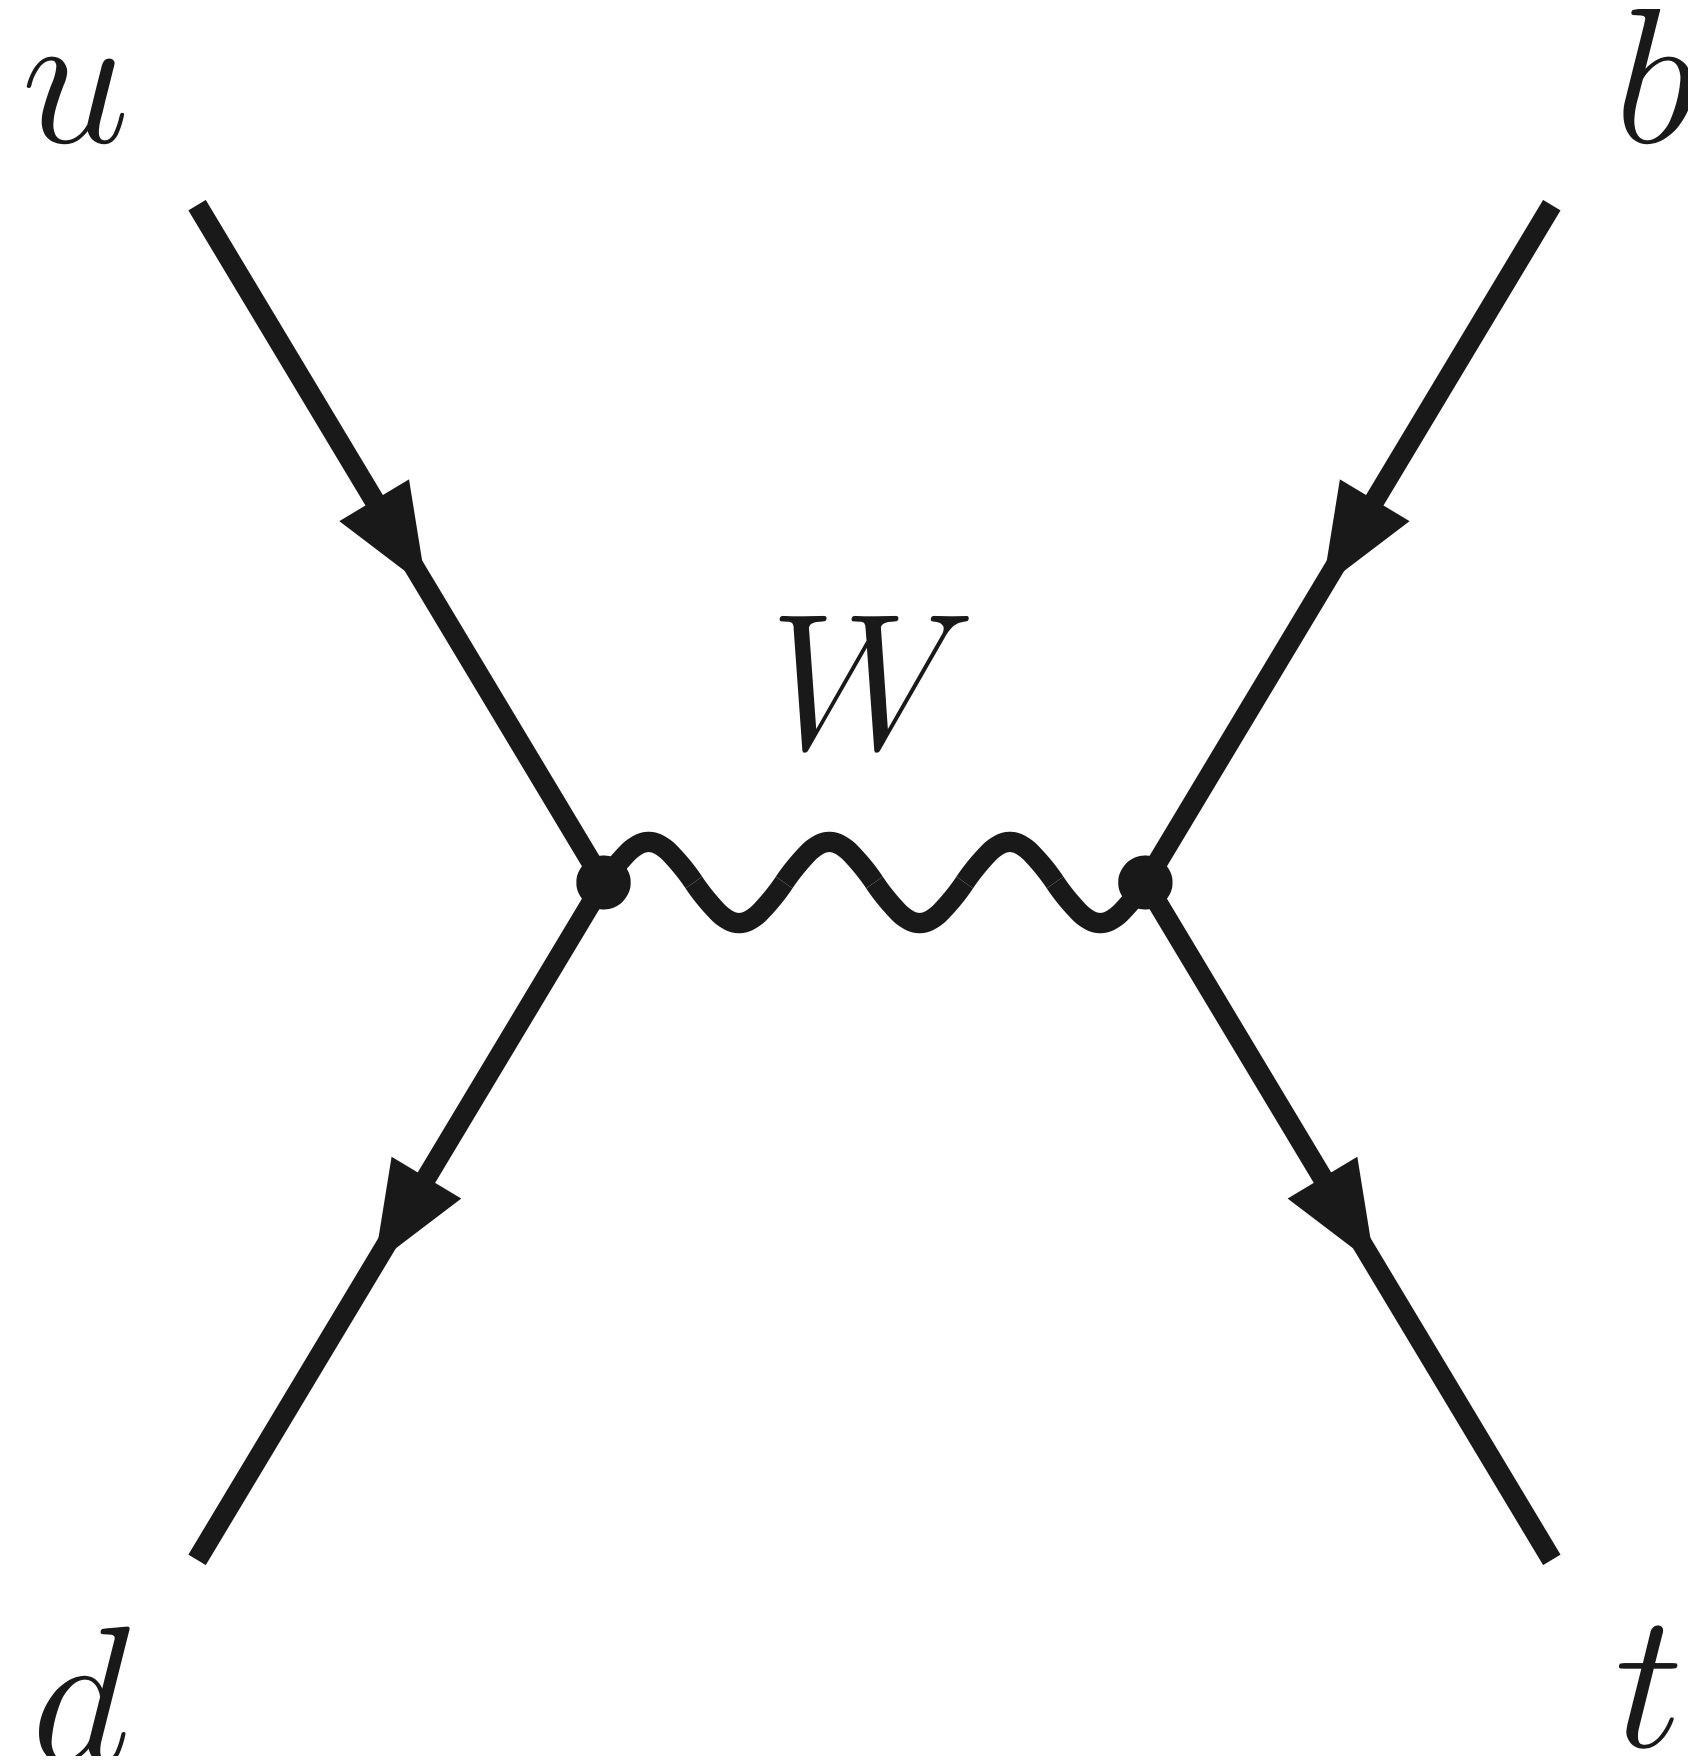
\includegraphics[width = 0.34\textwidth]{Chapter1/Single-top-schannel}
%    \caption{Representative Feynman diagram for the single-top-quark production in the \schannel.}
%    \label{fig:Chap1:top:singletop:schannel}
%\end{figure}

\begin{figure}
     \centering
     \begin{subfigure}[b]{0.3\textwidth}
         \centering
         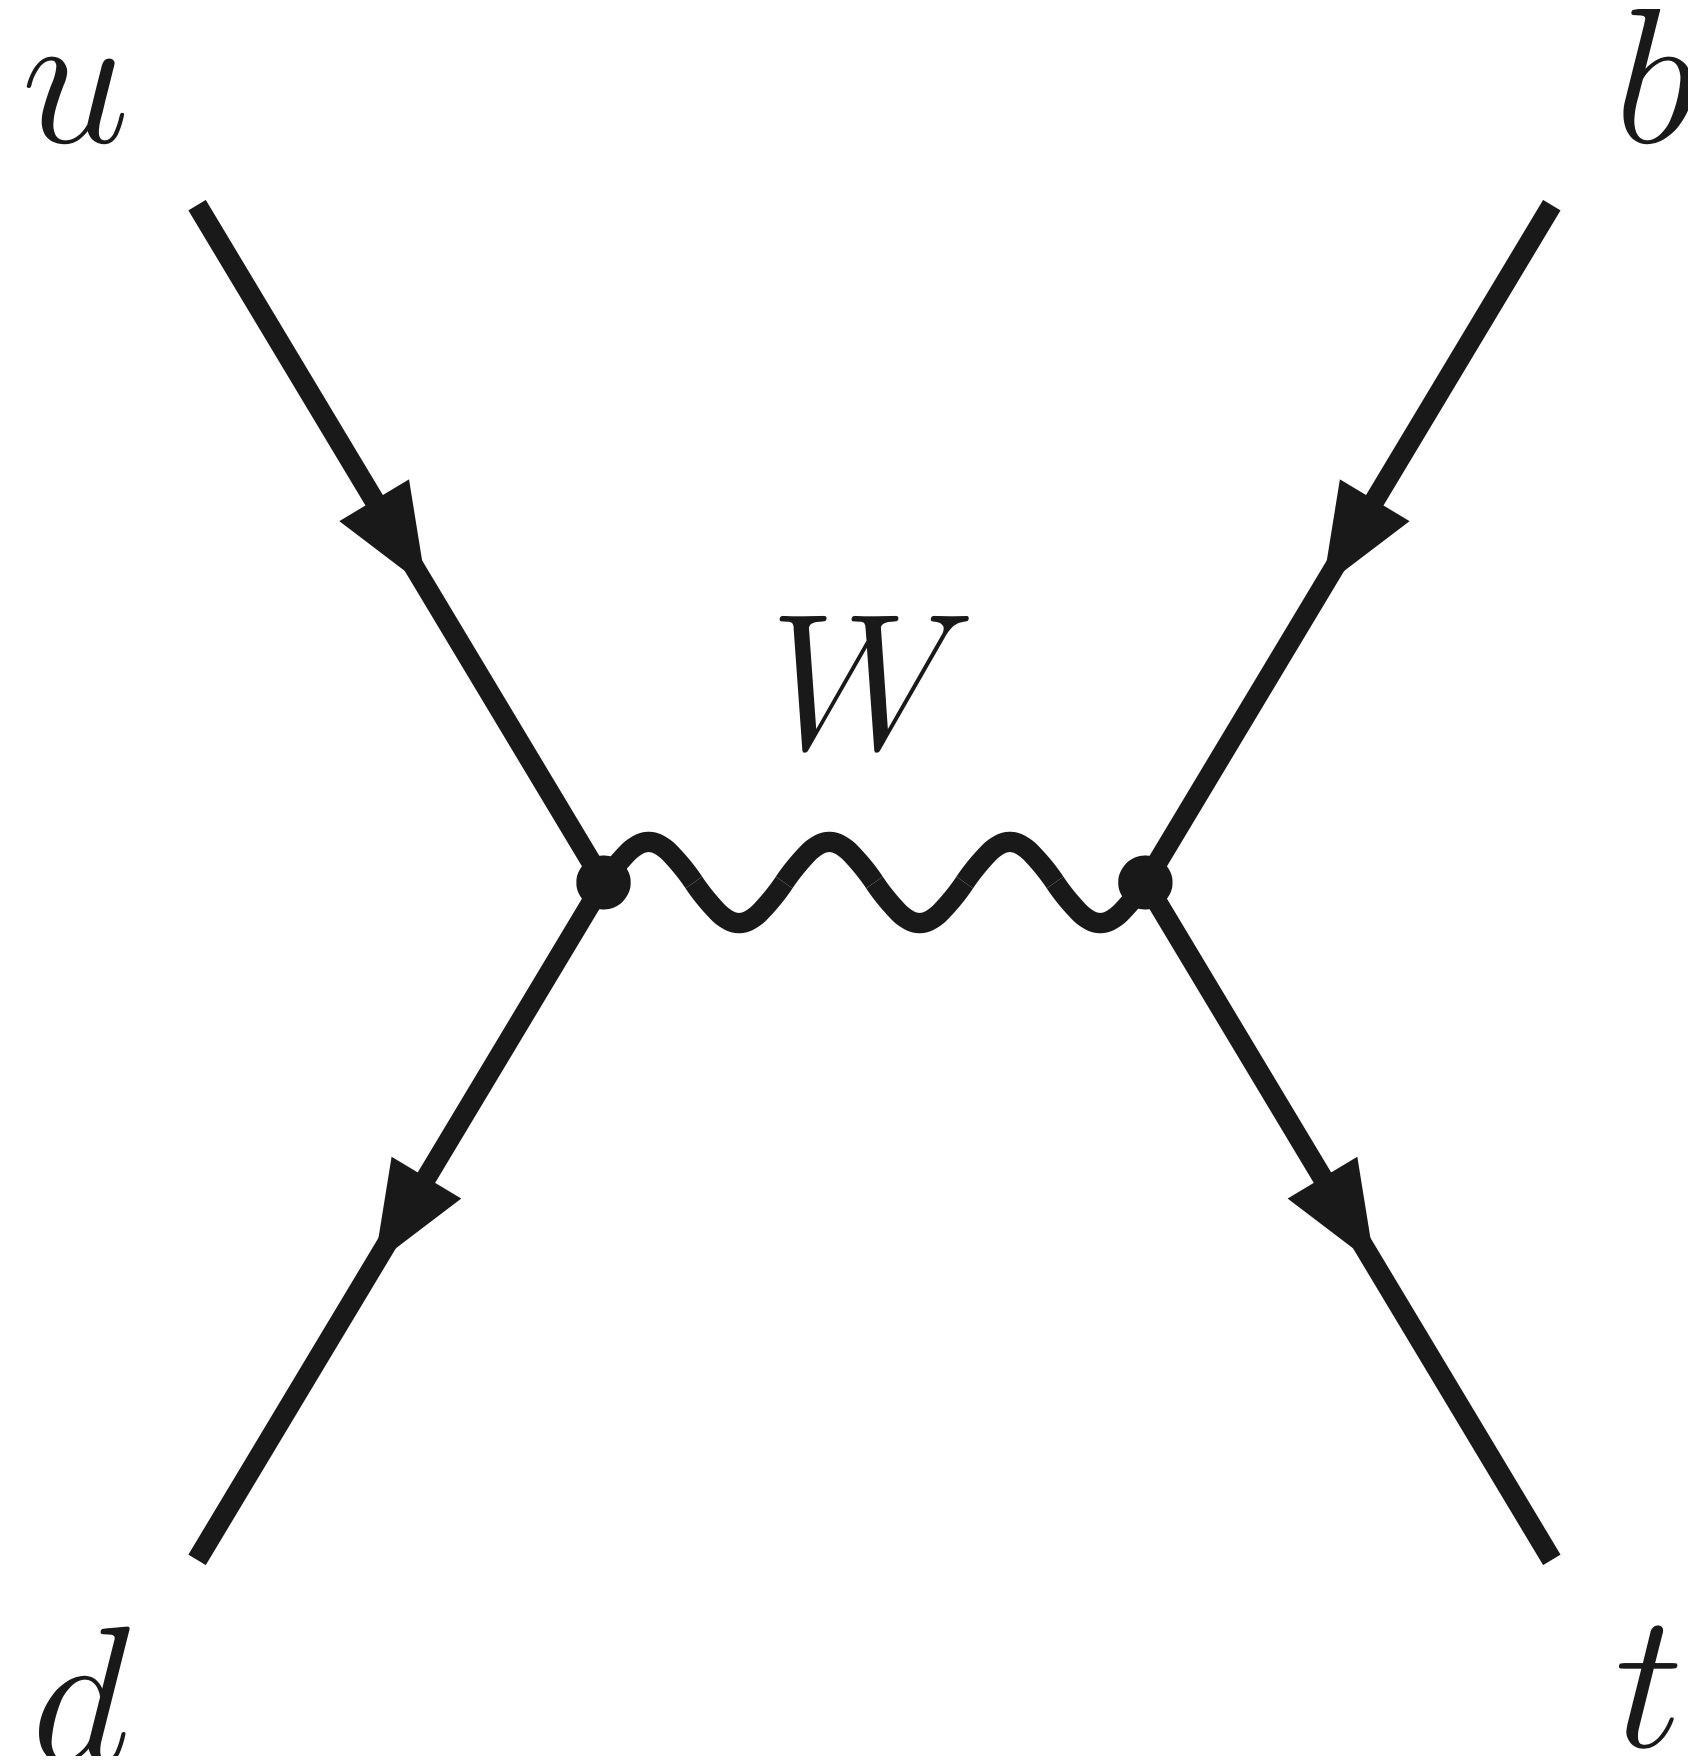
\includegraphics[width=\textwidth]{Chapter1/Single-top-schannel}
         \caption{}
         \label{fig:Chap1:top:singletop:schannel}
     \end{subfigure}
     \begin{subfigure}[b]{0.3\textwidth}
         \centering
         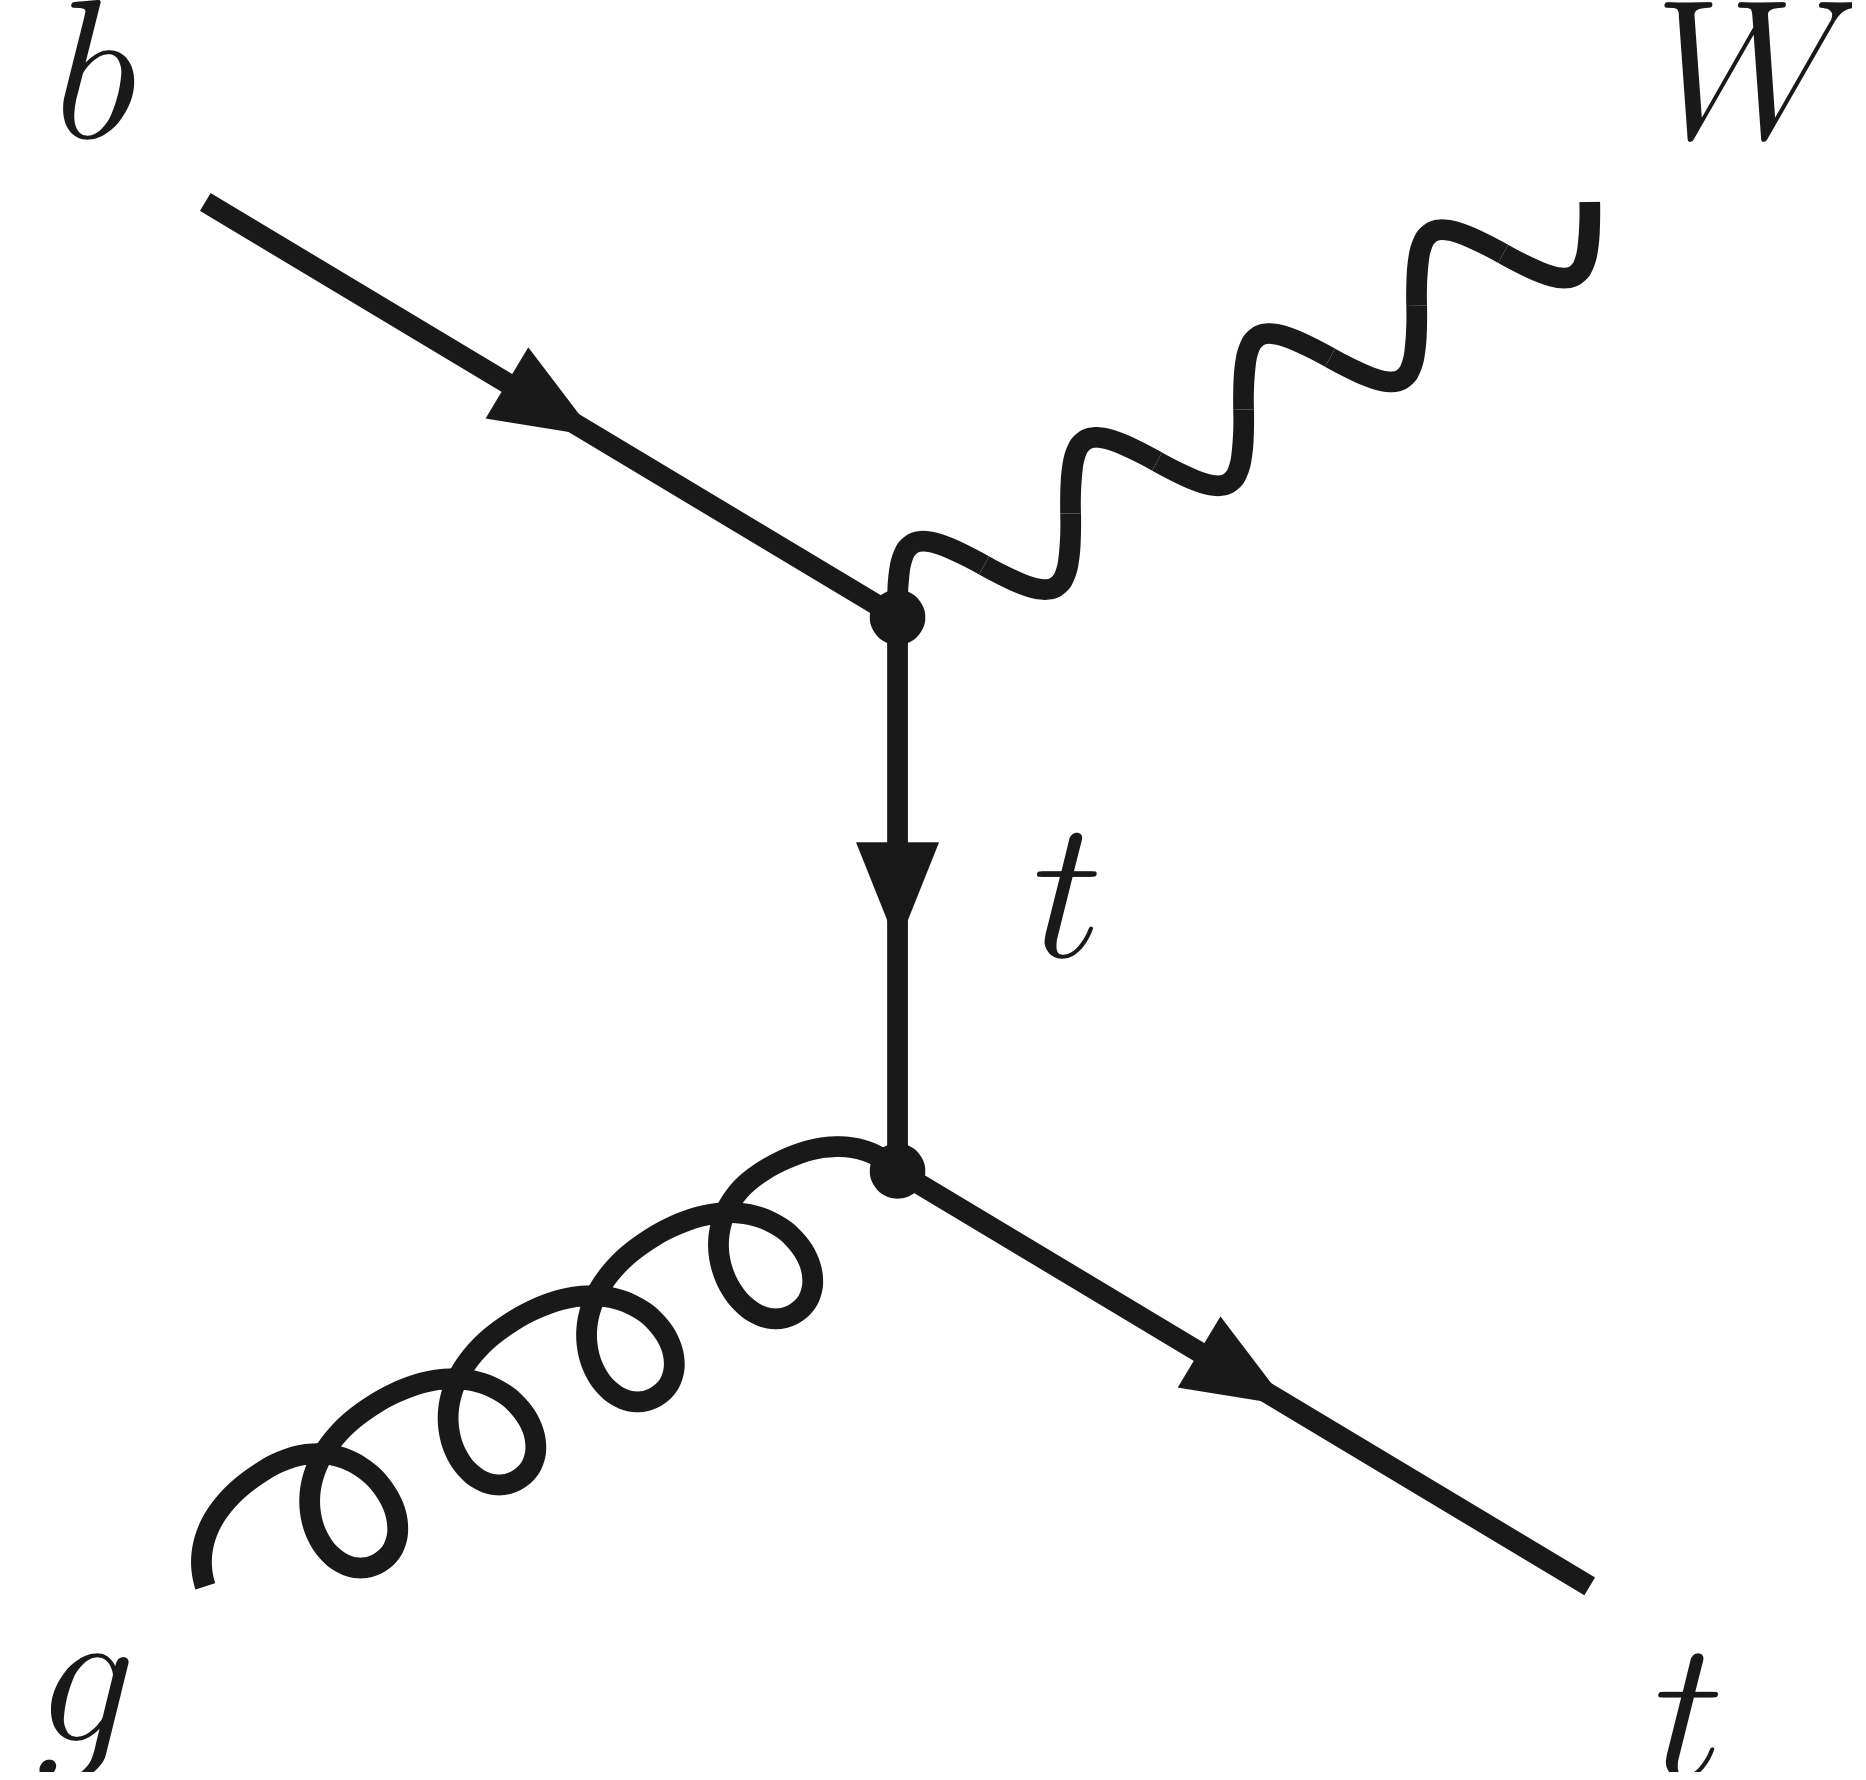
\includegraphics[width=\textwidth]{Chapter1/Single-top-Wt-A}
         \caption{}
         \label{fig:Chap1:top:singletop:tW_A}
     \end{subfigure}
     \begin{subfigure}[b]{0.3\textwidth}
         \centering
         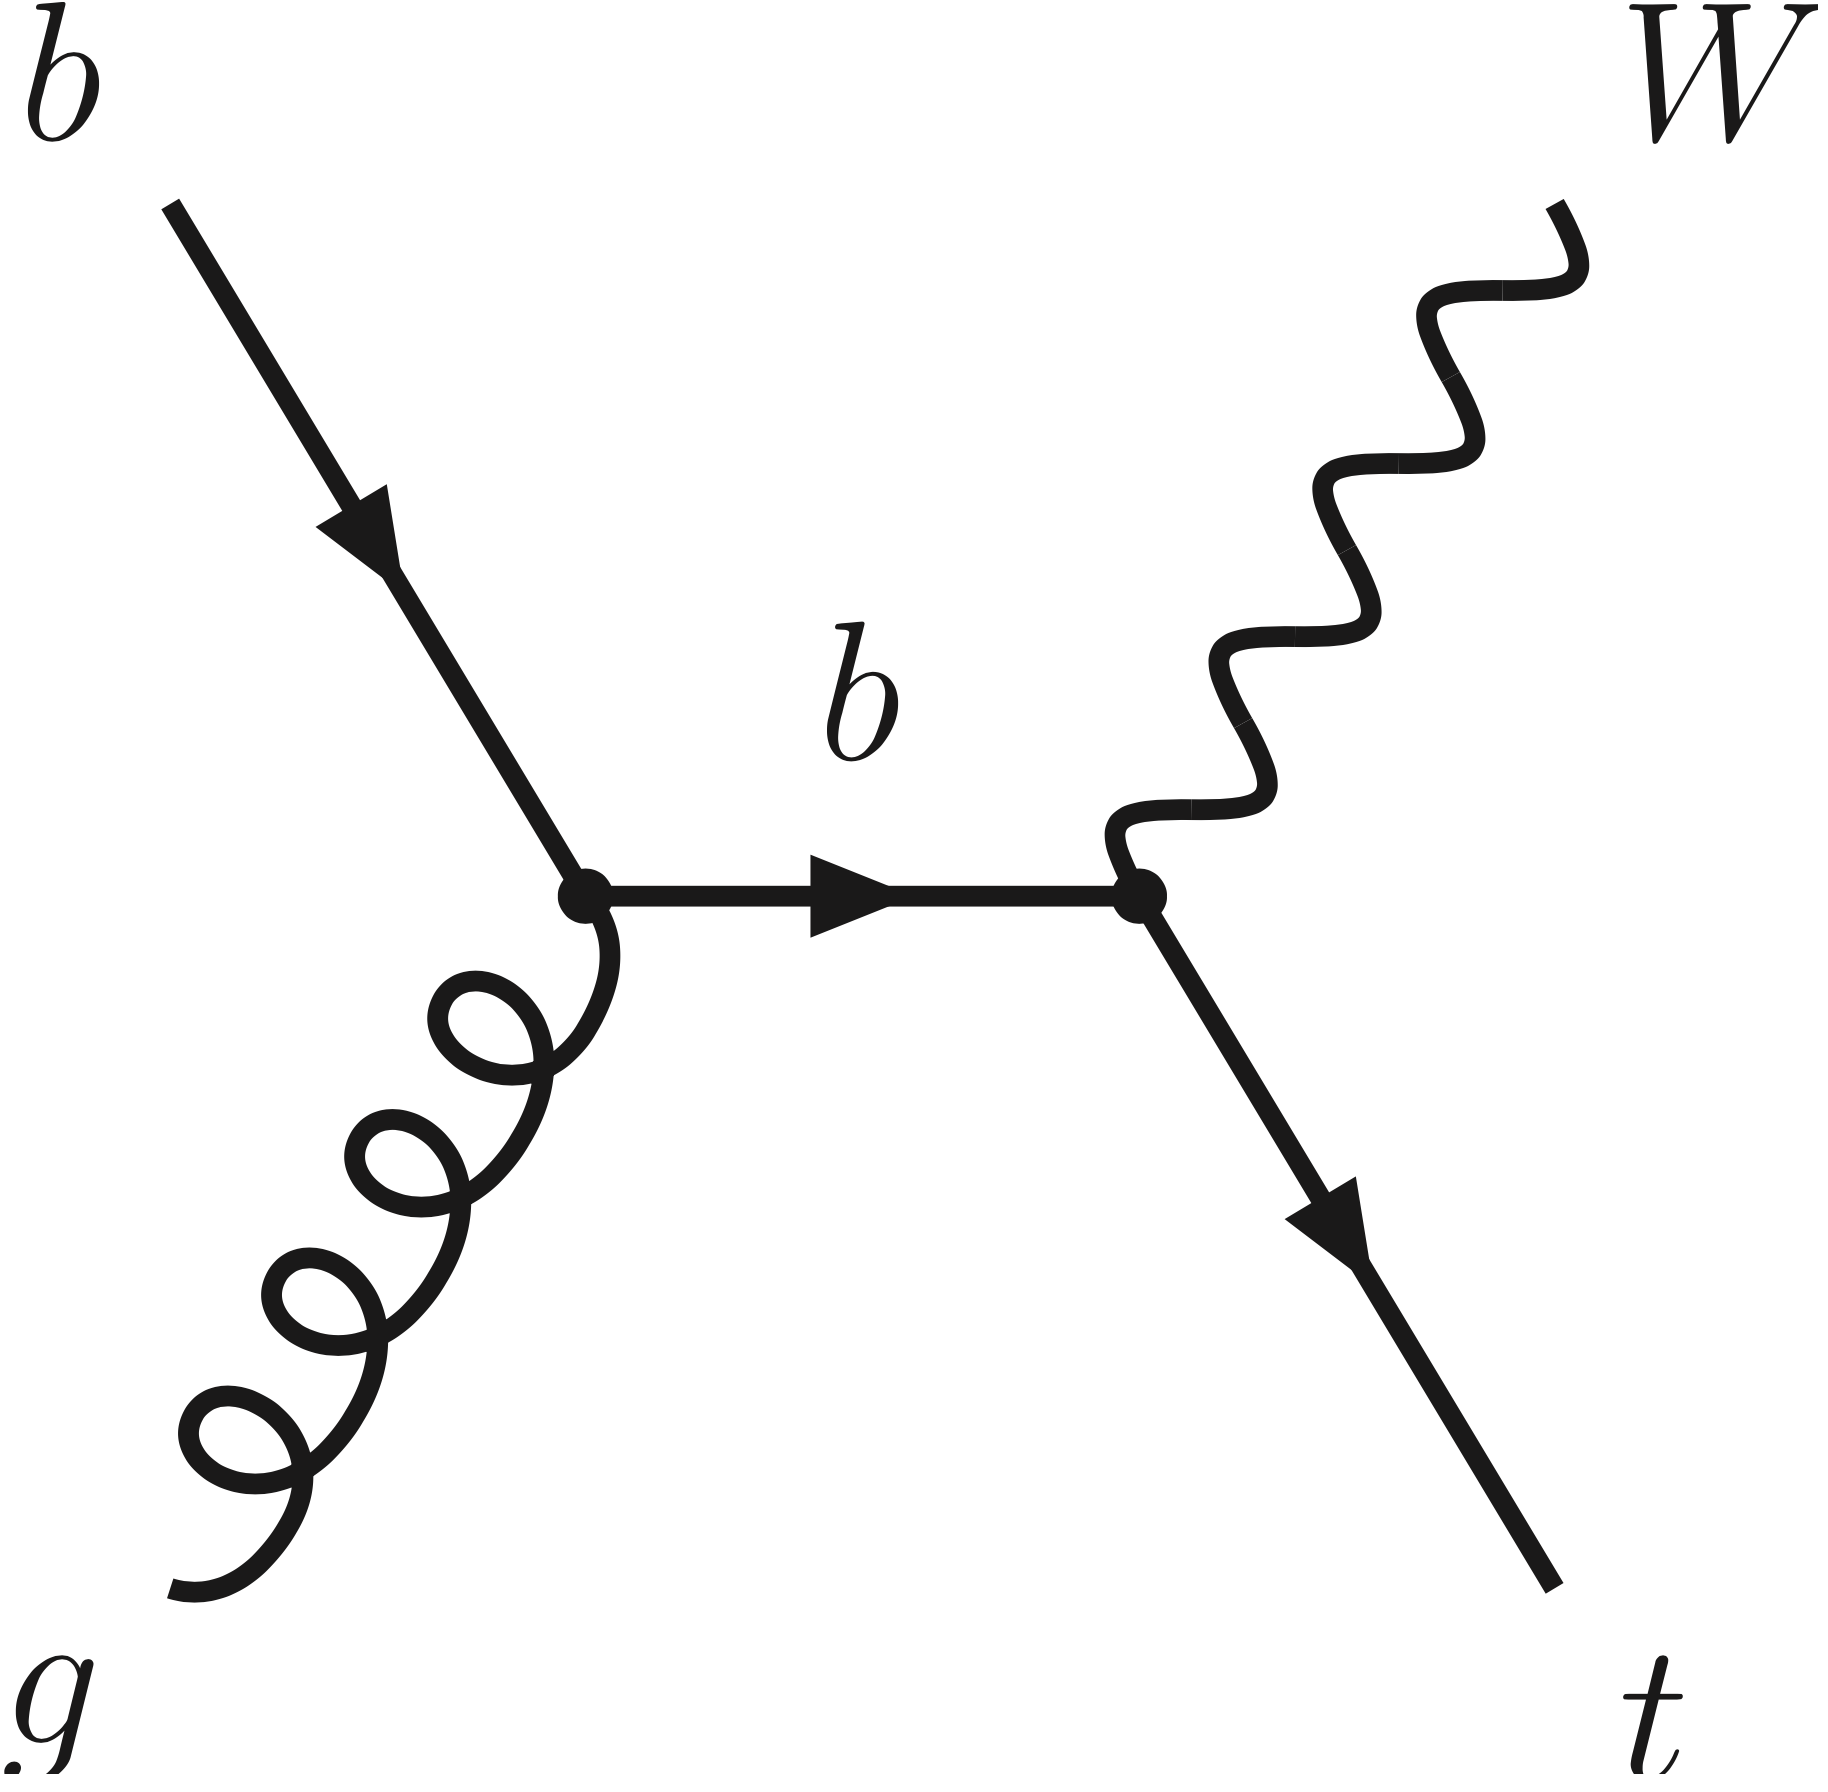
\includegraphics[width=\textwidth]{Chapter1/Single-top-Wt-B}
         \caption{}
         \label{fig:Chap1:top:singletop:tW_B}
     \end{subfigure}
        \caption{Representative Feynman diagrams for the single-top-quark production in (a) the \schannel
        and with (b, c) an associtared \PW boson. While the first one is not observed, the $\Ptop\PW$ is one the backgrounds
        in the \tHq analysis.}
        \label{fig:Chap1:top:singletop:SchannelAndAssocited}
\end{figure}


Although while at the LHC only an evidence\footnote{The threshold for "evidence" corresponds to 
p-value=0.003 (three standard-deviations) while the standard for "discovery" is 
p-value=0.0000003 (five standard-deviations). \pablo{Review this p-values}}
of the \schannel production has been found~\cite{ATLAS:2022wfk}, for Tevatron it was a
a significant part of the total single-top cross-section~\cite{Cremonesi:2014dma}. 
% Table 4 of https://citeseerx.ist.psu.edu/viewdoc/download?doi=10.1.1.205.6486&rep=rep1&type=pdf


%%%     Single-top quark   :::  associated Wt-channel
\paragraph{Associated $\Ptop\PW$}\mbox{}\\
%\begin{minipage}[t]{0.5\linewidth}
Finally, the associated production of a single top quark with a \PW boson 
(sometimes referred to as $\Ptop\PW$-channel) is represented by two the Feynman 
diagrams in Figures \ref{fig:Chap1:top:singletop:tW_A} and \ref{fig:Chap1:top:singletop:tW_B}.
To these two diagrams, the charge conjugate processes could be added to 
complete the $\Ptop\PW$ mechanisms. 
The predicted cross-section for the associated $\Ptop\PW$ is
$\sigma^{pred}_{tW, \Ptop + \APtop} = 71.7 \pm 5.2 \,\textrm{pb}$. This and 
all $\sigma$ in this section are calculated for a top mass of $\mtop = 172.5$~GeV.

Cross-section measurements for the associated $\Ptop\PW$ production 
performed by ATLAS and CMS at $13$~TeV have found
 $\sigma_{tW} = 94^{+38}_{-32} \,\textrm{pb}$~\cite{ATLAS:2016ofl}
and $\sigma_{tW} = 79.2 \pm 8.9\,\textrm{pb}$~\cite{CMS:2022xey} respectively. 
Both results are compatible with the NLO +NNLL prediction.
%\begin{equation*}
	%\sigma_{tW, \Ptop + \APtop} &= 71.7 \pm 1.80 (\textrm{scale}) \pm 3.40(\textrm{PDF}+\alpha_{s})\,\textrm{pb.}
%	\sigma_{tW, \Ptop + \APtop} = 71.7 \pm 5.2 \,\textrm{pb.}
%\end{equation*}

%and NLO in QCD with \HATHOR v.2.1. The PDF and $\alpha_{s}$ uncertainties are calculated
%using the PDF4LHC prescription~\cite{Butterworth:2015oua} with the 
%MSTW2008 68\% CL NLO~\cite{Martin:2009iq, Martin:2009bu}, CT10 NLO~\cite{Lai:2010vv} 
%and NNPDF2.3~\cite{Ball:2013hta} PDF sets, added in quadrature to the scale uncertainty.
%The measurements for the associated $\Ptop\PW$ are shown in Figure~\ref{fig:Chap1:top:singletop:tW_CrossSection}.
%The associated $\Ptop\PW$ production is an important background in the studies of the Higgs boson.
%\end{minipage} \hfill
%\begin{minipage}[t]{0.4\textwidth}
%\setbox0=\hbox{T} % tallest letter of the first line of other minipage
%\vskip-\ht0
%\begin{figure}
	%\begin{wrapfigure}{r}{0.45\textwidth}
%	    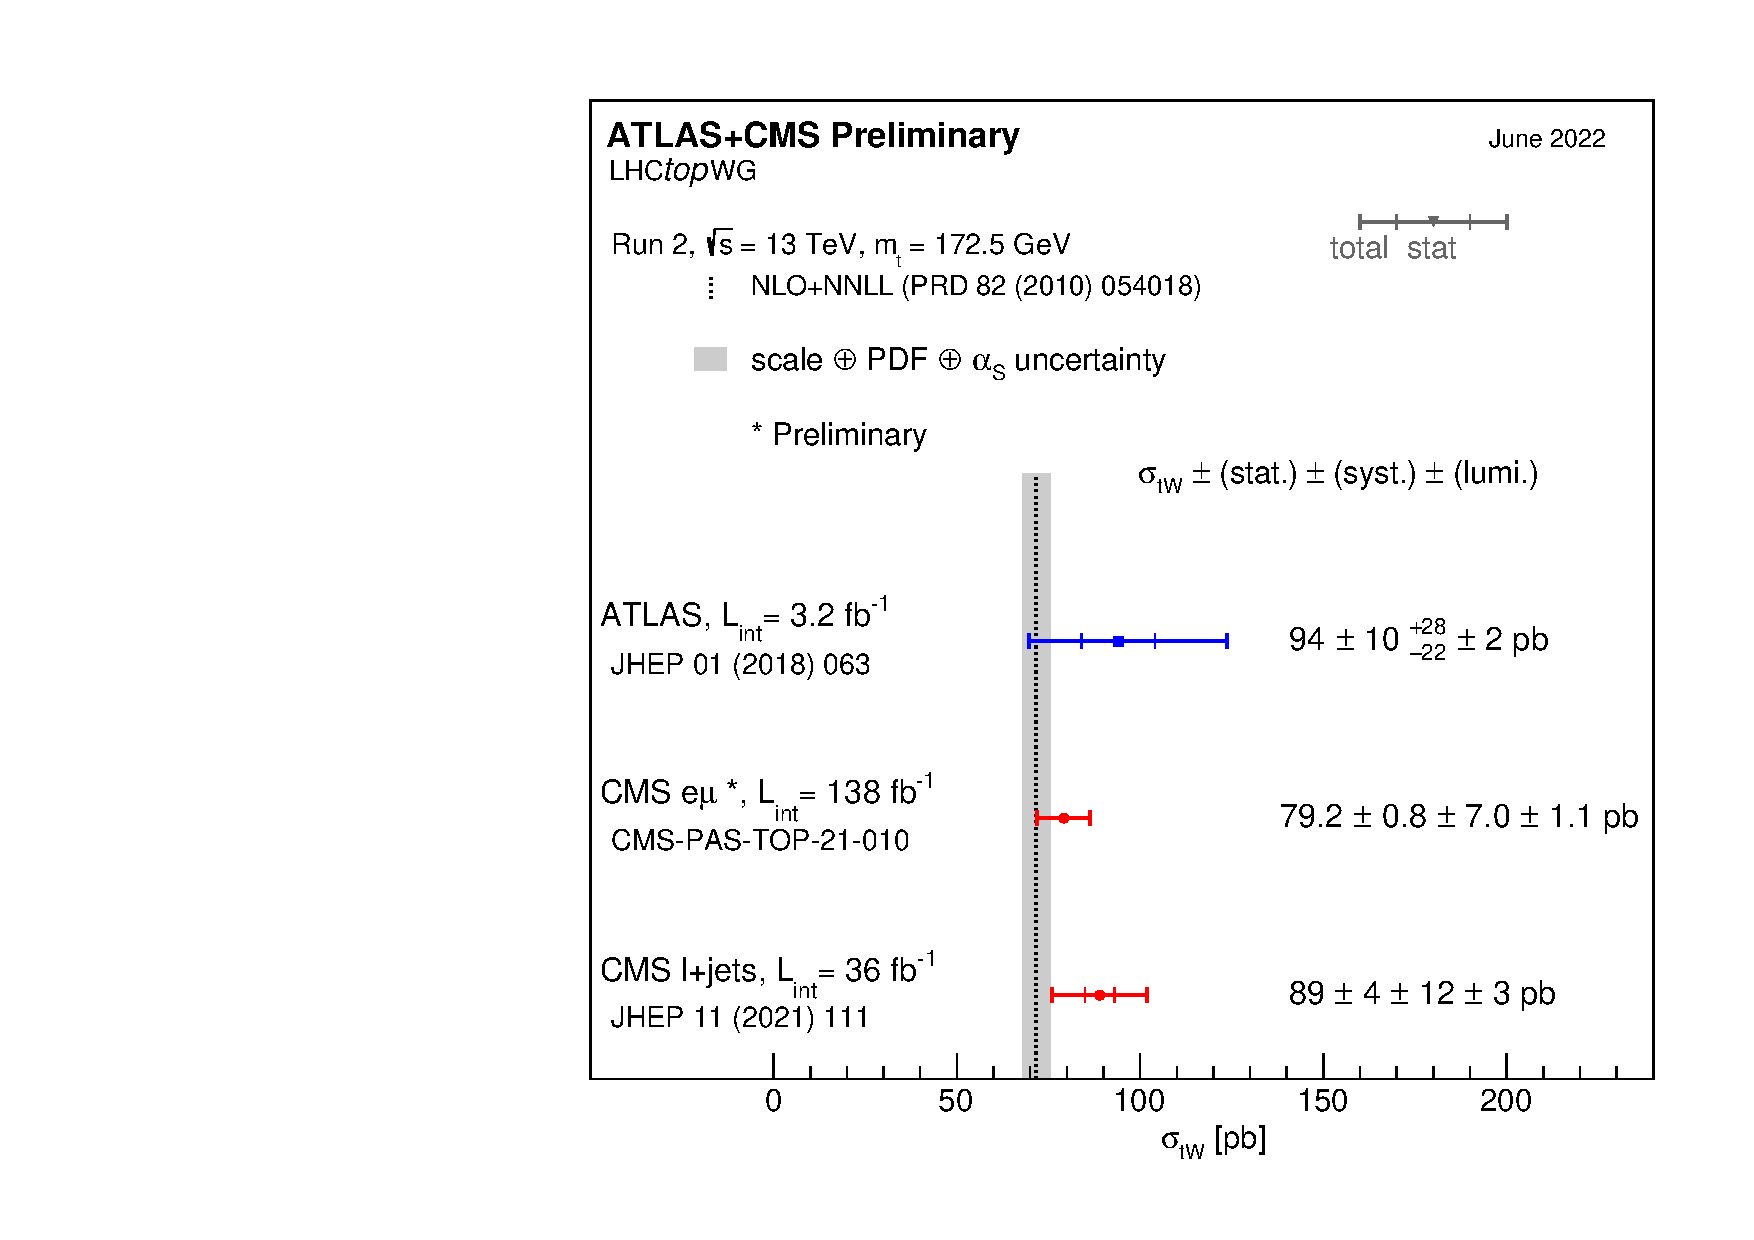
\includegraphics[width = 0.95\linewidth]{Chapter1/singletop_tW13_jun22}
% 	   \captionof{figure}{Cross-section measurements for the associated $\Ptop\PW$ production boson 
%	   performed by ATLAS and CMS at $13$~TeV, and combined result compared 
%	   with the NLO + next-to-next-to-leading logarithmic (NNLL) prediction.
%	   \pablo{Quitar tabla y poner resultados en el párrafo.}}
%   	 \label{fig:Chap1:top:singletop:tW_CrossSection}
	 %\end{wrapfigure}
%\end{figure}
%\end{minipage}


%\begin{figure}
%     \centering
%     \begin{subfigure}[b]{0.3\textwidth}
%         \centering
%         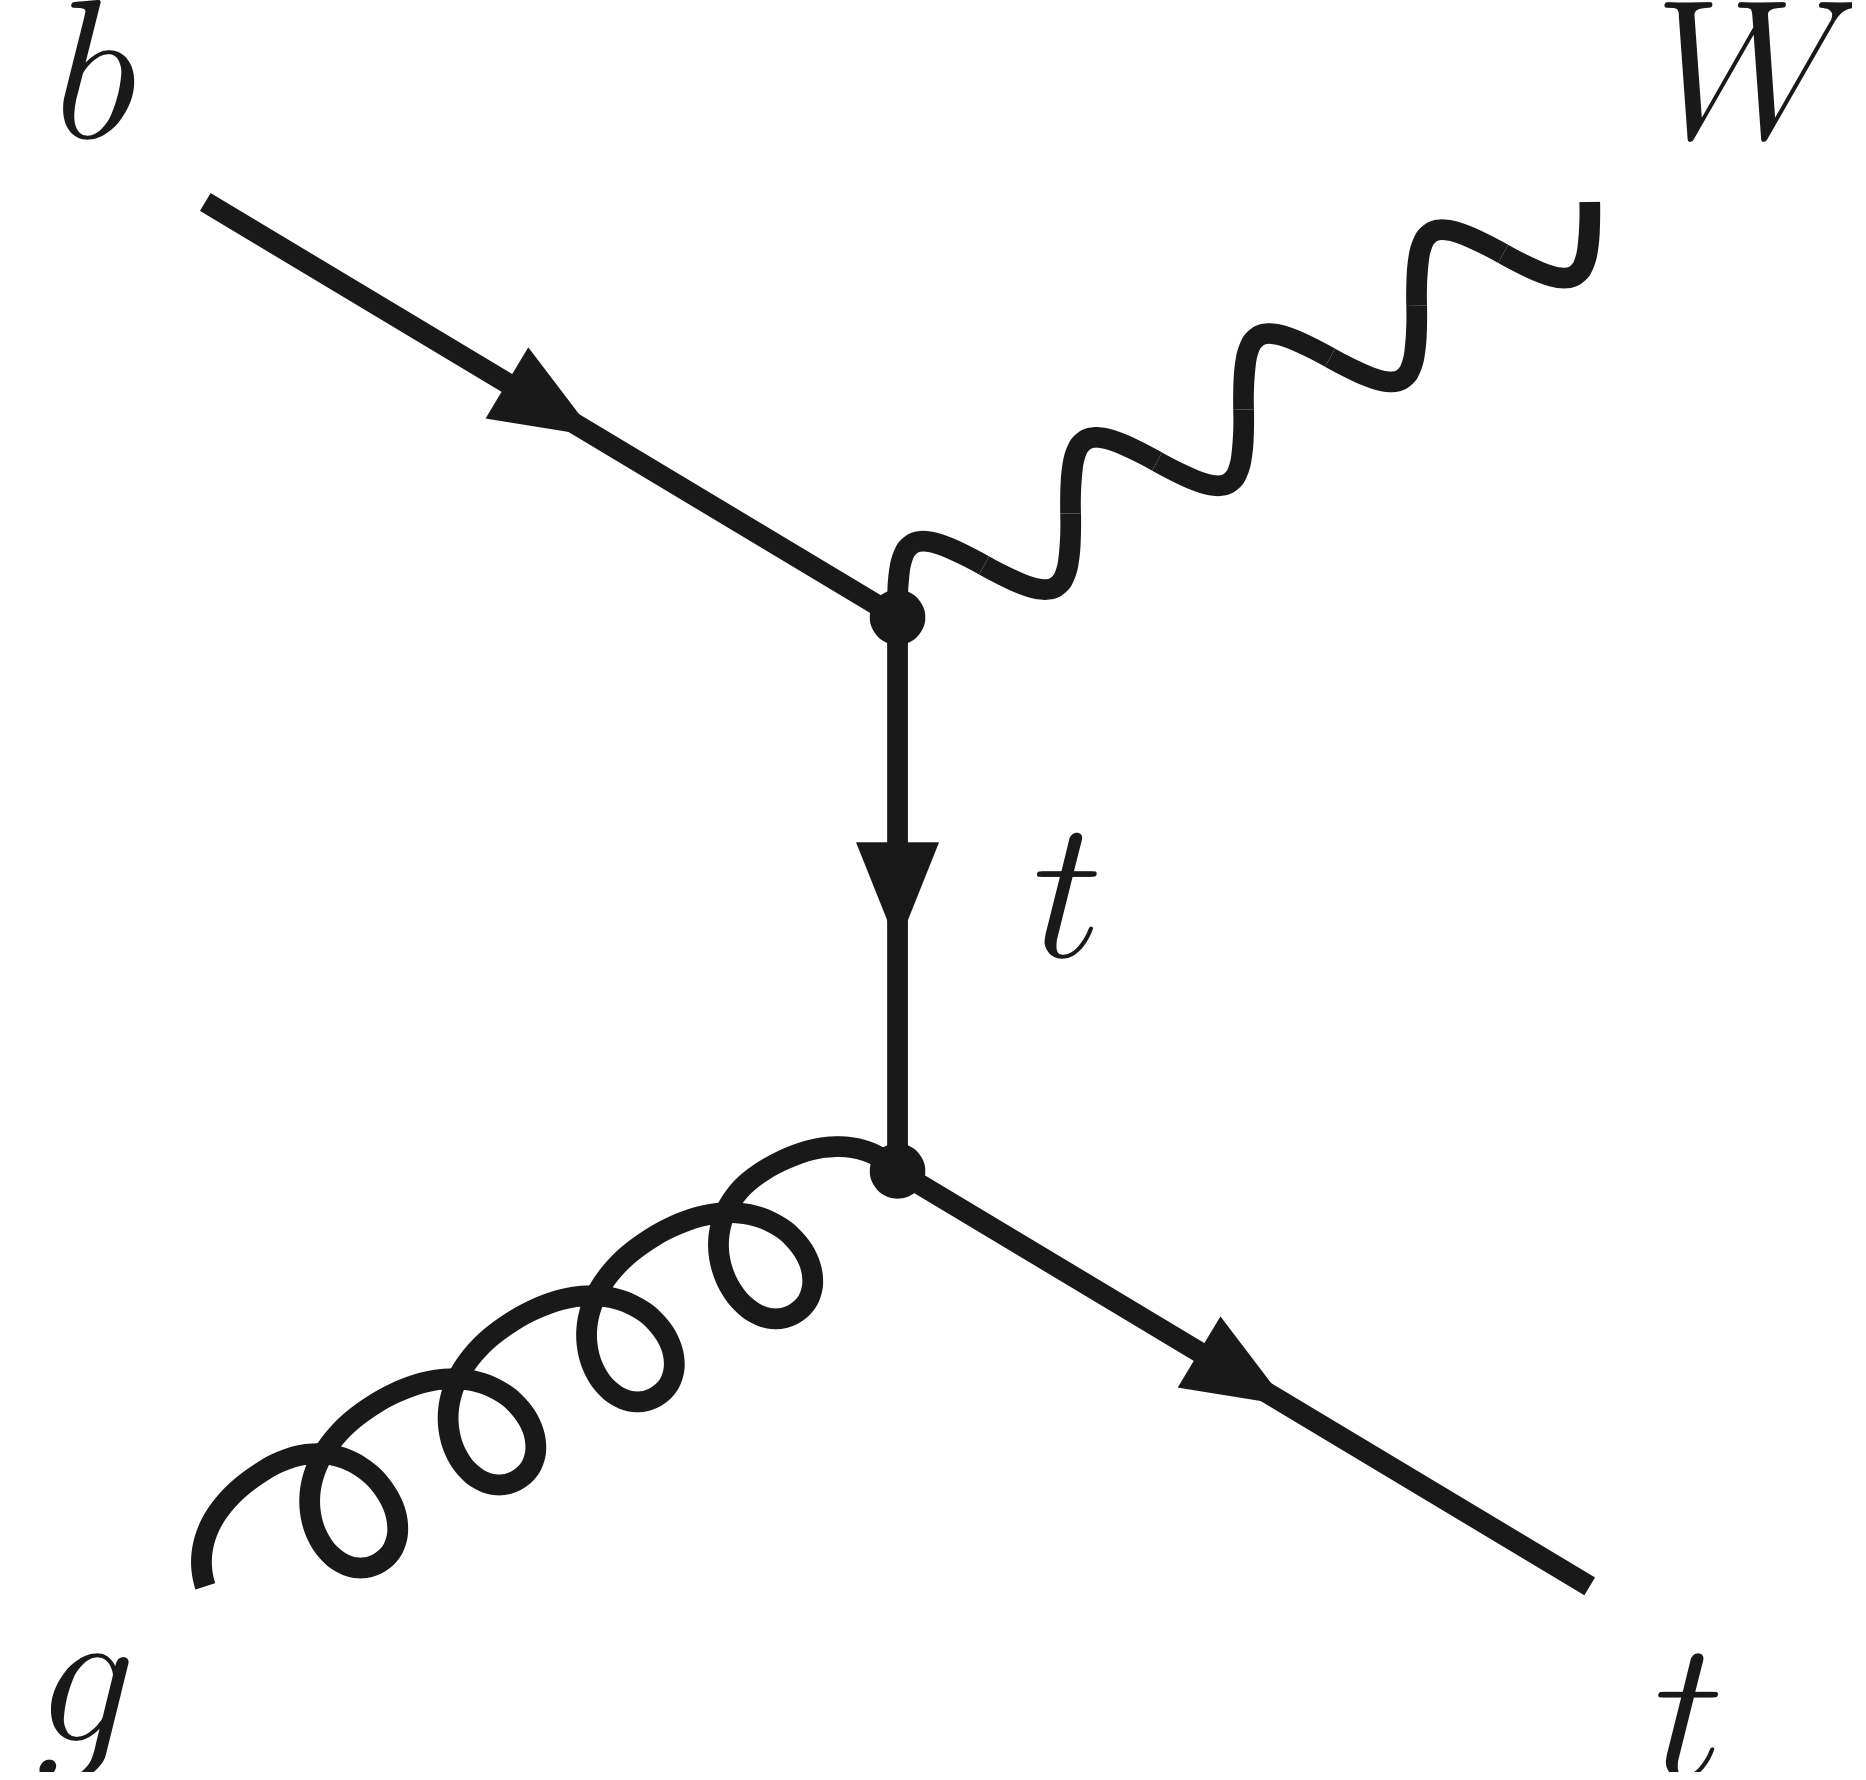
\includegraphics[width=\textwidth]{Chapter1/Single-top-Wt-A}
%         \caption{}
%         \label{fig:Chap1:top:singletop:tW_A}
%     \end{subfigure}
%     \begin{subfigure}[b]{0.3\textwidth}
%         \centering
%         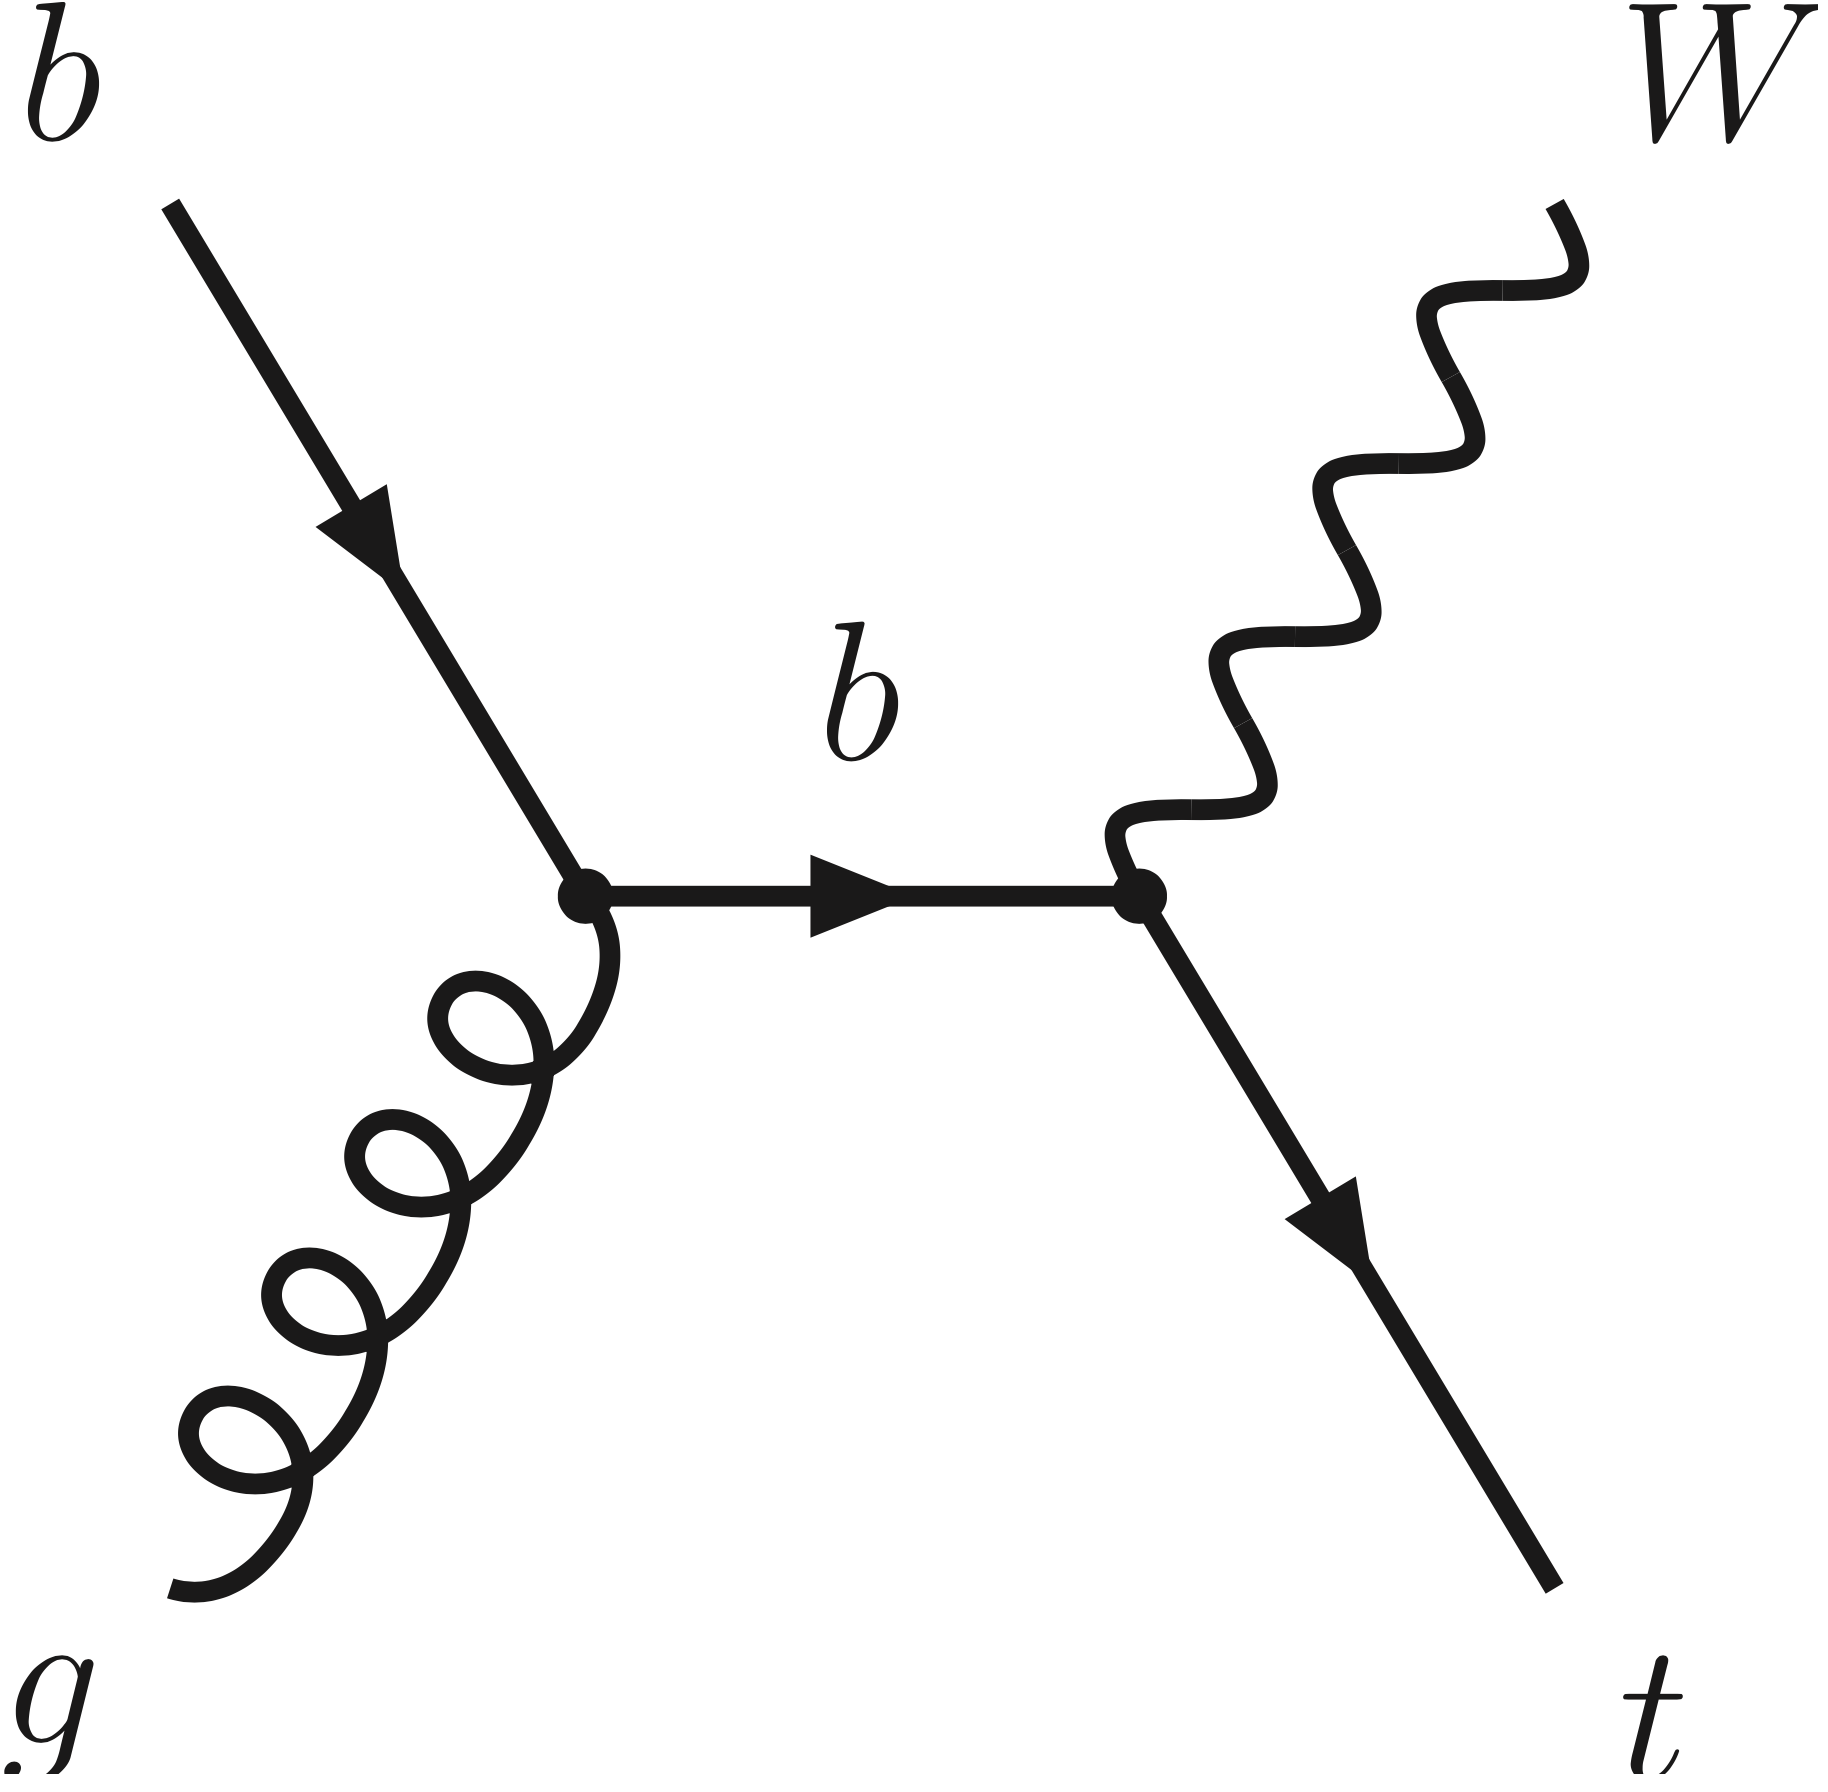
\includegraphics[width=\textwidth]{Chapter1/Single-top-Wt-B}
%         \caption{}
%         \label{fig:Chap1:top:singletop:tW_B}
%     \end{subfigure}
%        \caption{Representative Feynman diagrams for the single-top-quark production in association with a \PW boson.}
%        \label{fig:Chap1:top:singletop:tW}
%\end{figure}
%\end{comment}





%%%%%%%%%%%%%%%%
%                Four tops               %
%%%%%%%%%%%%%%%%
\subsubsection{Four tops}
\label{sec:Chap1:Top:Production:4tops}
%source: 
%		https://inspirehep.net/files/216bcad412f9e5d56fda0820c1b726c9
%		https://atlas.web.cern.ch/Atlas/GROUPS/PHYSICS/CONFNOTES/ATLAS-CONF-2020-013/
The production of four top quarks ($t\bar{t}t\bar{t}$) is a rare SM process that takes place at the LHC 
with a predicted cross-section of $\sigma^{pred}_{t\bar{t}t\bar{t}} = 12.0^{+2.2}_{-2.5}$~fb for \Pproton\Pproton
collisions at $\CM=13$~TeV (calculations at NLO for QCD and EW~\cite{Frederix:2017wme}). 
ATLAS and CMS have measured the $t\bar{t}t\bar{t}$ production cross-section and obtained,
respectively, $\sigma_{t\bar{t}t\bar{t}} = 24^{+16}_{-14}$~fb~\cite{ATLAS:2021kqb} and 
$\sigma_{t\bar{t}t\bar{t}} = 12.6^{+5.8}_{-5.3}$~fb~\cite{CMS:2019rvj}.
While the first measurement does not agree with the theoretical prediction, 
it yields a larger statistical significance. 

% Remove summary plots and Feynman diagrams for the tttt
%\begin{comment}
Figure~\ref{fig:Chap1:top:4top_xsec} presents the $\sigma_{t\bar{t}t\bar{t}}$ measurements 
by ATLAS and CMS compared to the quoted theoretical calculation. 

The representative Feynman diagrams are presented in Figure~\ref{fig:Chap1:top:4Top:Feyn}, 
where of particular interest is the production by the exchange of a Higgs boson. 
This indicates a strong dependence of this type of production
with the top-quark-Yukawa coupling.

\begin{minipage}[t]{0.55\textwidth}
\begin{flushleft}
\noindent
\vskip0pt
	%\begin{figure}
    	%\centering
    	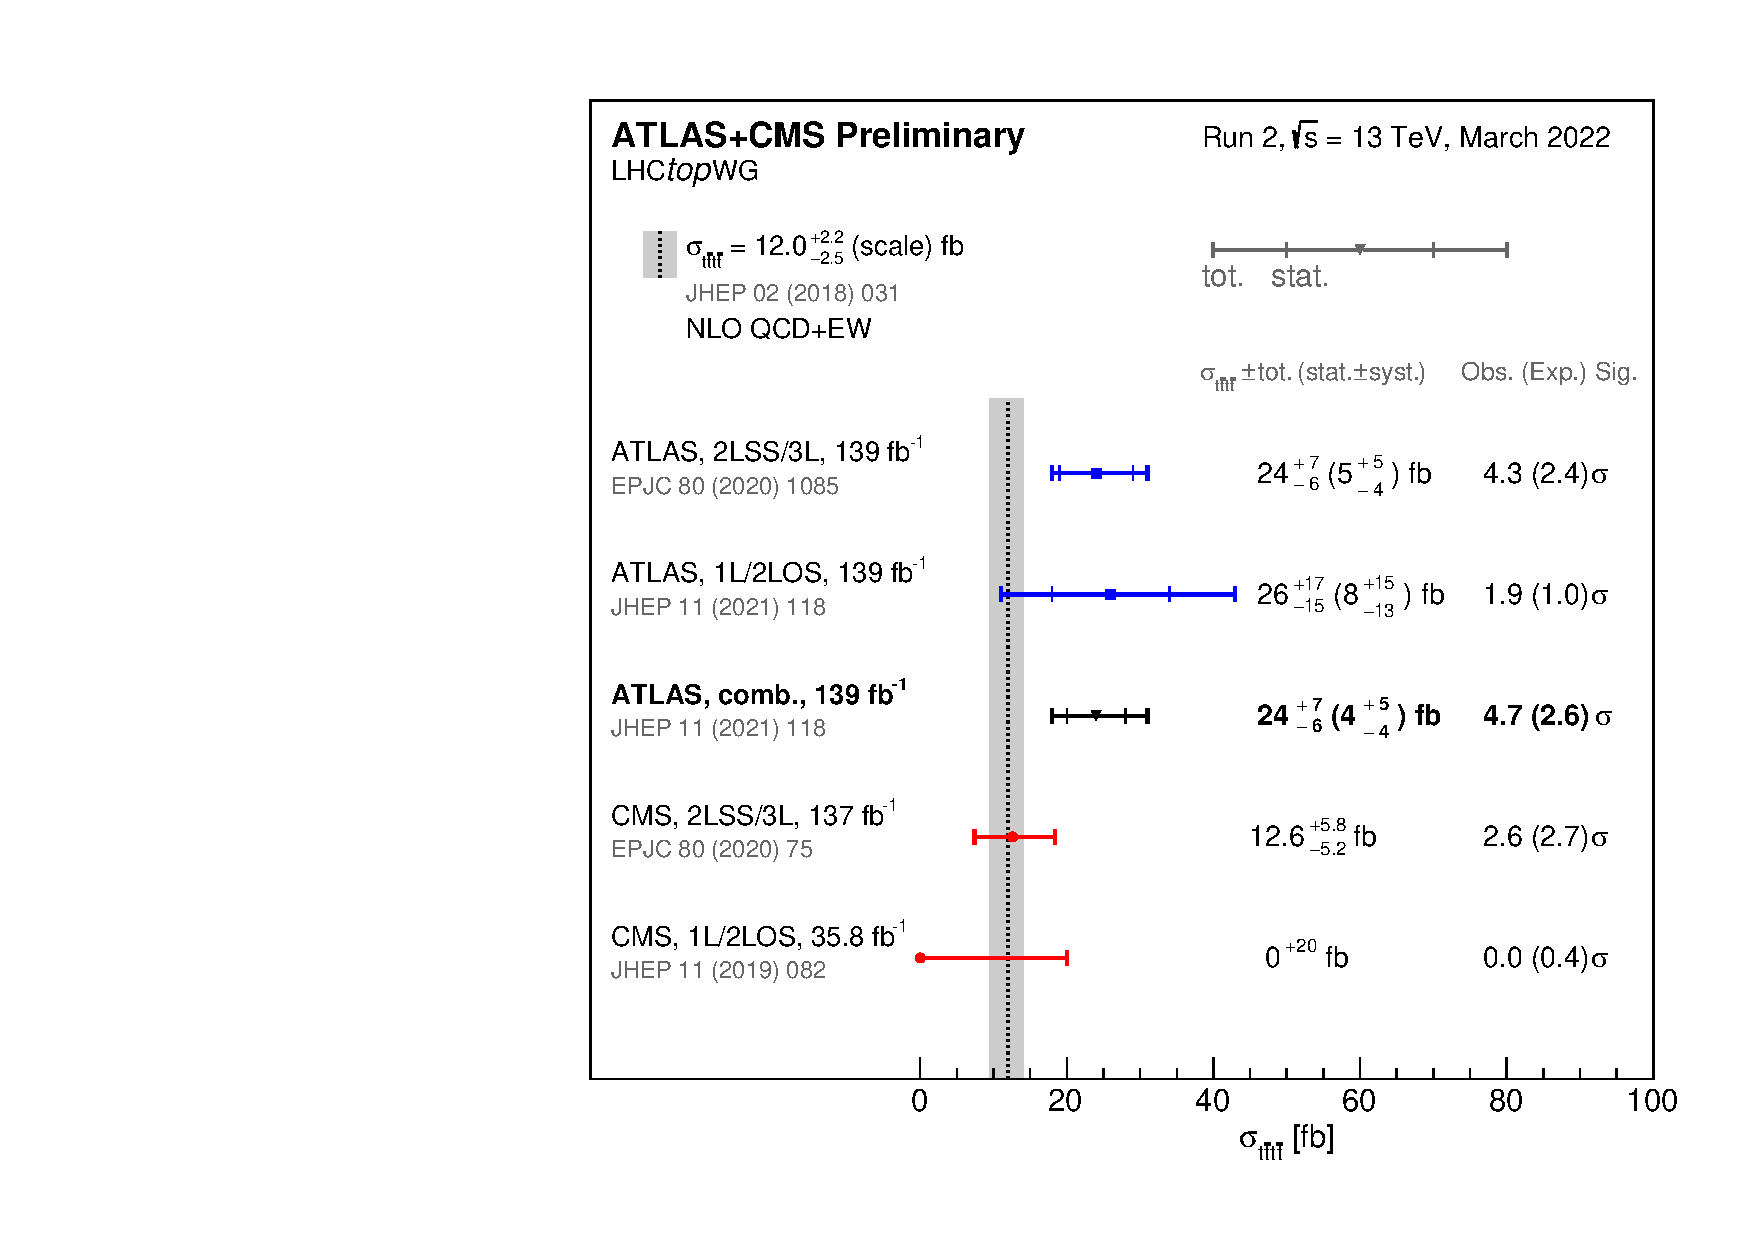
\includegraphics[width =\textwidth]{Chapter1/fourtop_summary_mar22}
    	\captionof{figure}{Summary of the ATLAS and CMS measurements of 
	the $t\bar{t}t\bar{t}$ production cross-sections at $13$~TeV in various channels.
	\pablo{Quitar figura, mencionar el resultado más preciso combinado de ATLAS y su significancia.}}
        \label{fig:Chap1:top:4top_xsec}
        \strut
	%\end{figure}
\end{flushleft}	
\end{minipage}\hfill
\begin{minipage}[t]{0.4\textwidth} 
%\setbox0=\hbox{T} % tallest letter of the first line of other minipage
\vskip0pt
	%\begin{multicols}{2}
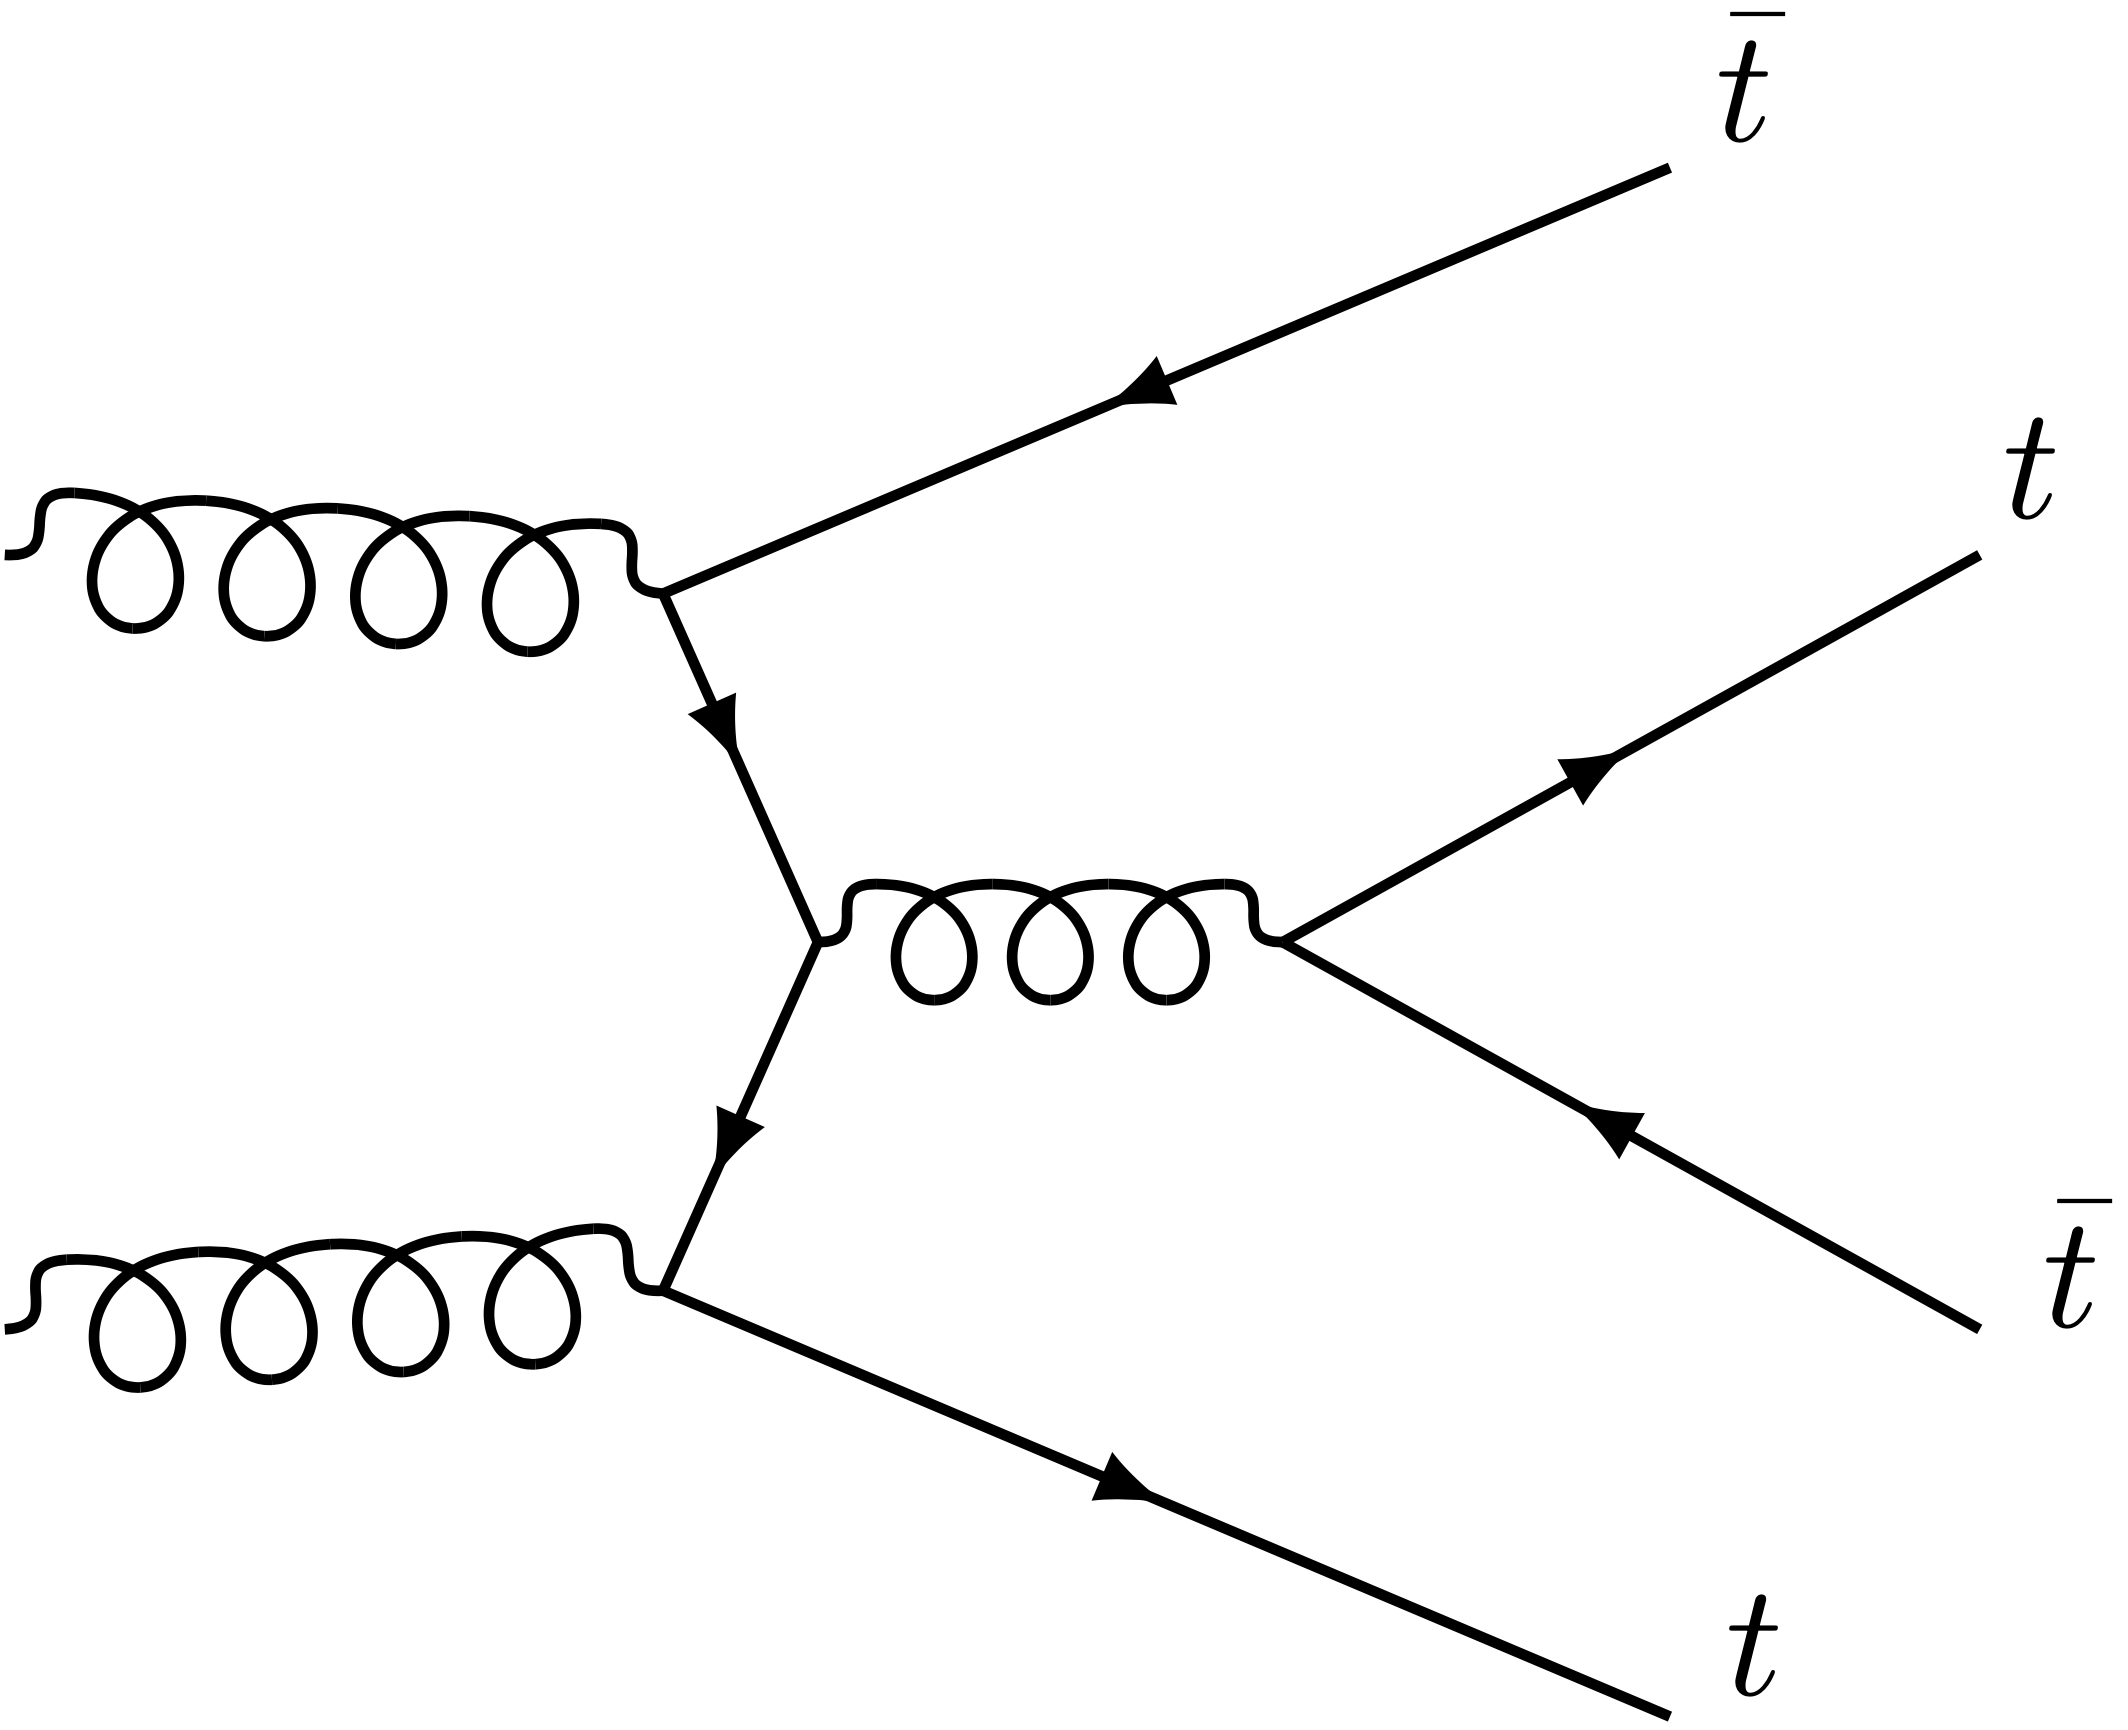
\includegraphics[width=0.85\linewidth]{Chapter1/Feynman_FourTop_A}\par 
    	%\end{multicols}
	%\begin{multicols}{2}
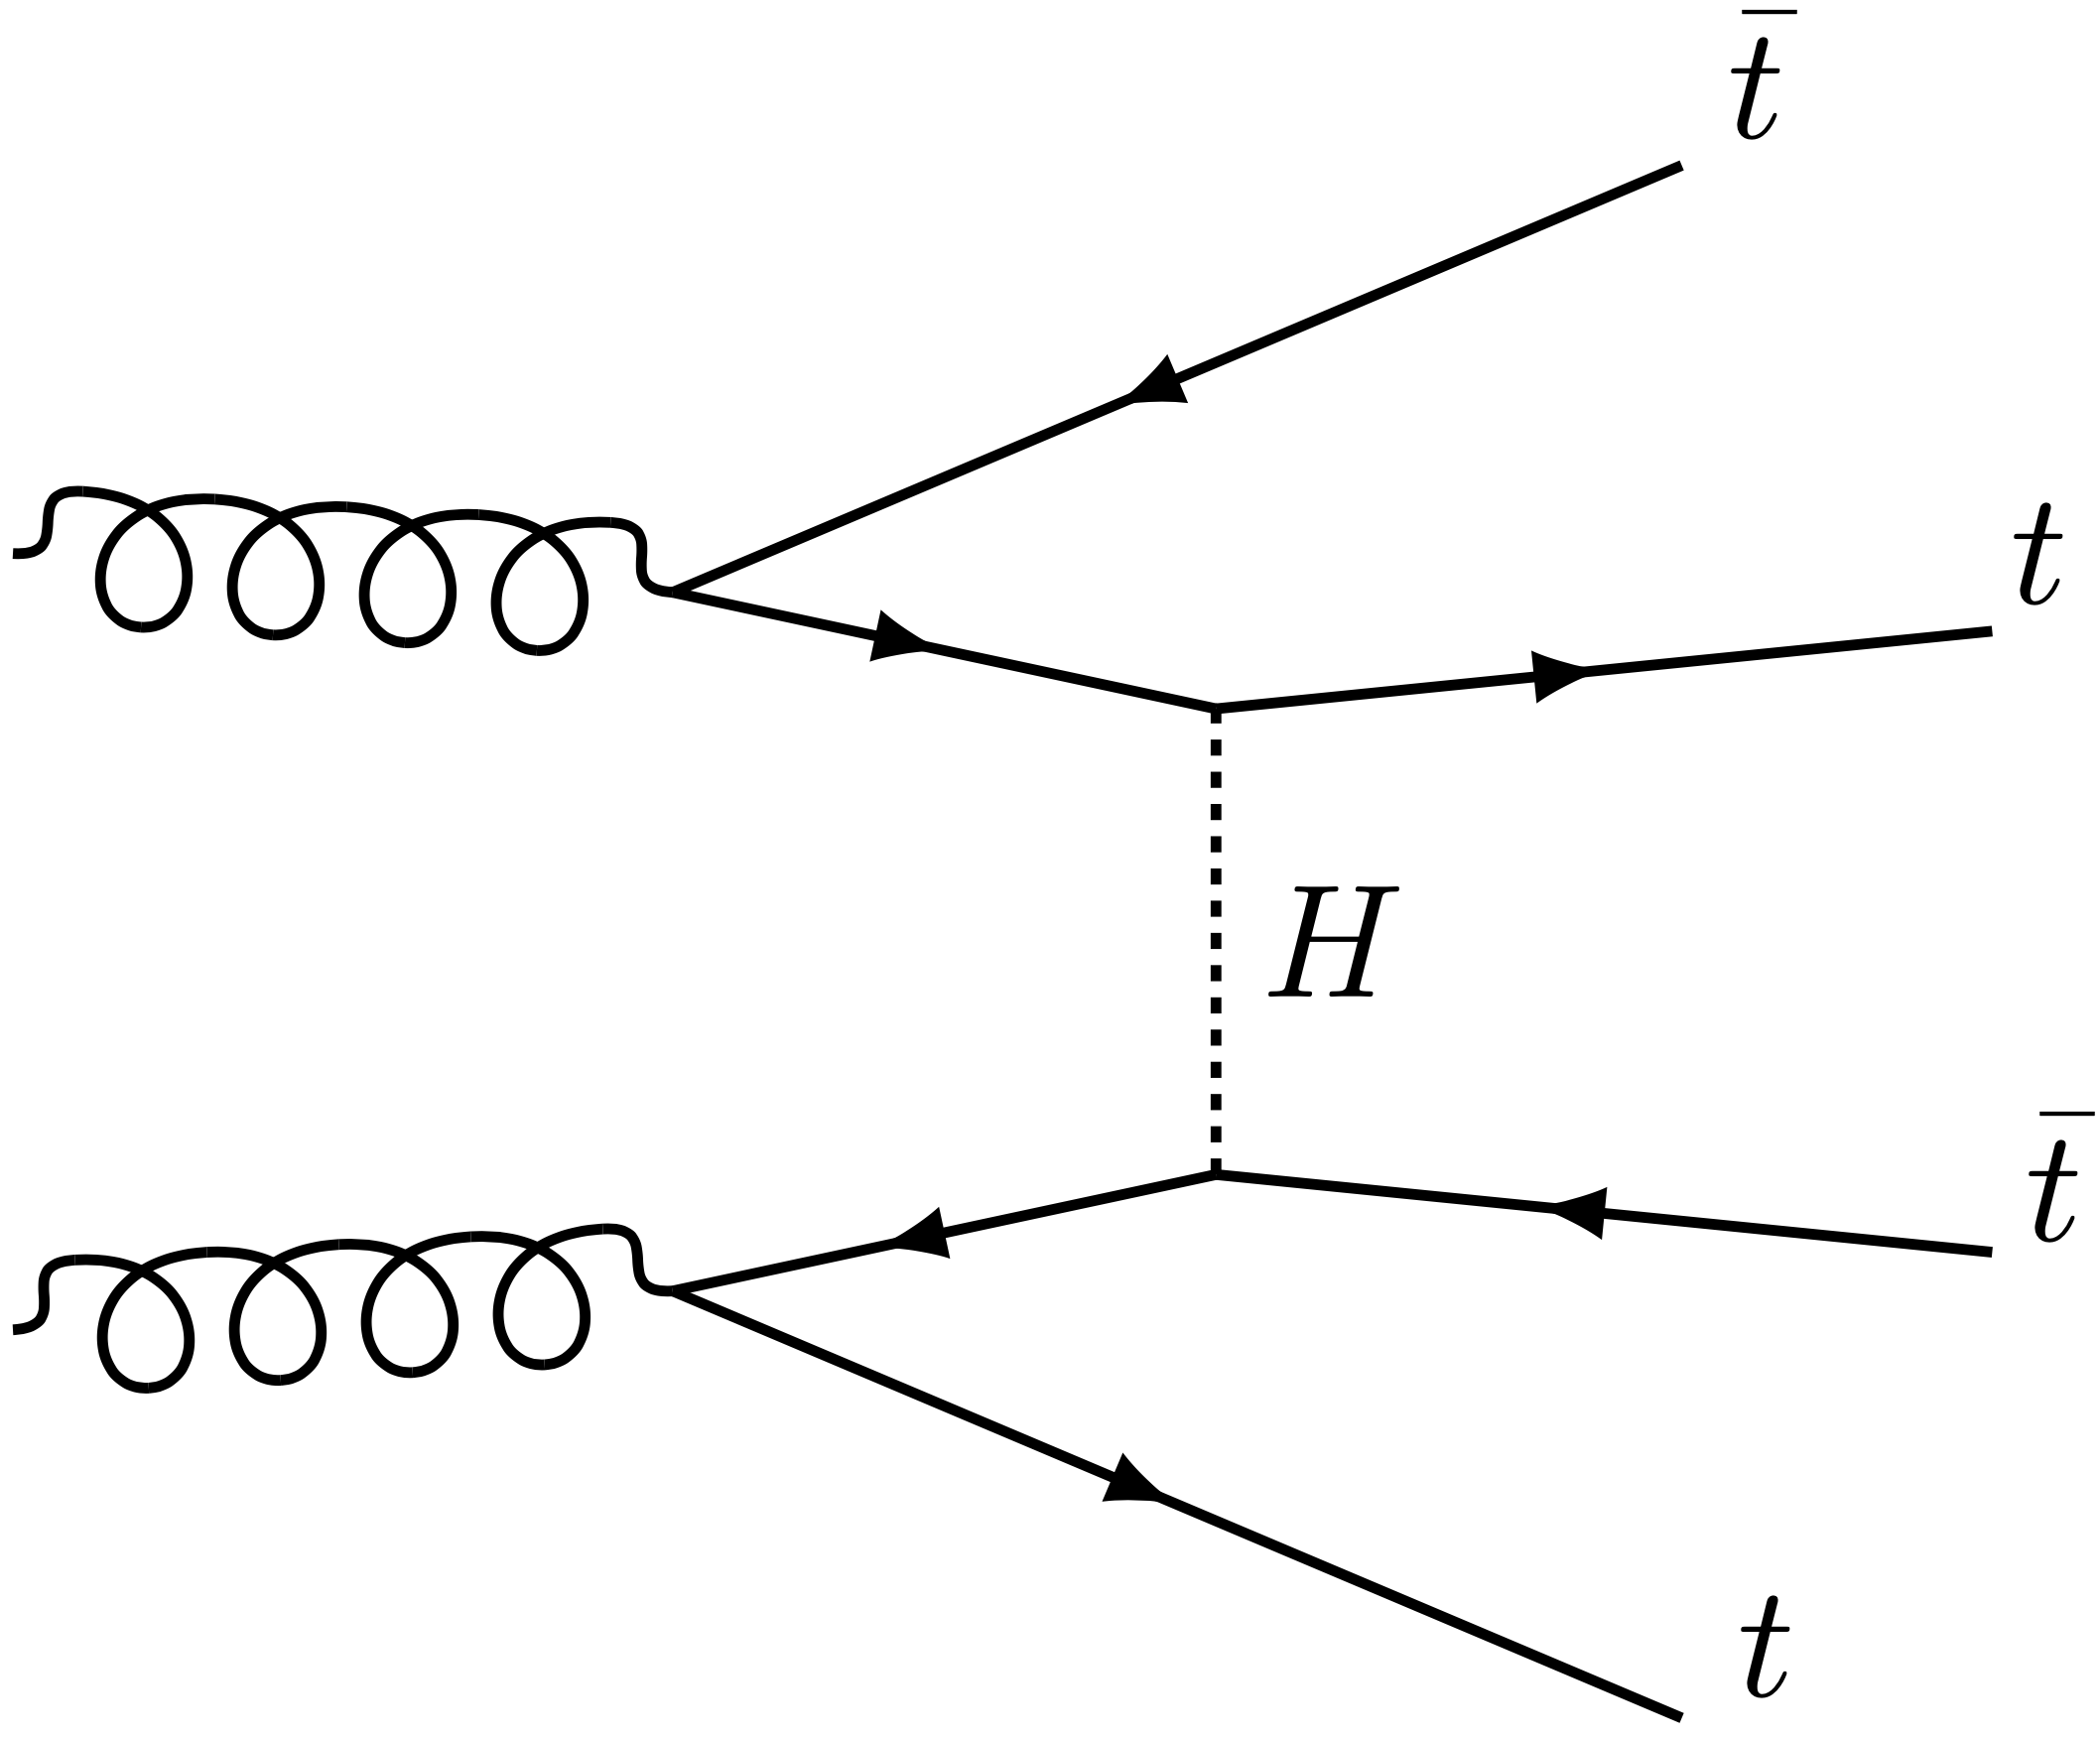
\includegraphics[width=0.85\linewidth]{Chapter1/Feynman_FourTop_B}\par
	%\end{multicols}
	\captionof{figure}{Representative Feynman diagrams for the $\Pgluon\Pgluon \rightarrow t\bar{t}t\bar{t}$ production.}
        \label{fig:Chap1:top:4Top:Feyn}
\end{minipage}
% Avoid the vertical space in the minipage envirorment:
% https://tex.stackexchange.com/questions/331617/too-much-vertical-space-before-a-minipage-environment
%\end{comment}

\end{comment}

%%%%%%%%%%%%%
%                tt-X              %
%%%%%%%%%%%%%
\subsubsection{Associated \ttX production}
\label{sec:Chap1:Top:Production:ttbar_plus_X}
% Measurements for top+X: https://atlas.web.cern.ch/Atlas/GROUPS/PHYSICS/PUBNOTES/ATL-PHYS-PUB-2022-049/
The associated-top-quark productions are important processes to measure
the coupling of the top quark to other particles of the SM. 
When a pair of top quarks is produced along with another particle 
the process is referred to as $\ttX$. The most relevant $\ttX$ productions
are those in which the pair is produced together with \PW, \PZ or \Pgamma bosons.
From these, \ttW and \ttZ play a role in the analysis carried in this thesis.
These two processes along with \ttbar are the three most relevant backgrounds
in one of the channels of the analysis performed in this thesis.
%in the \tHq production with two light leptons and one hadronic tau when
%the light leptons have the same electric charge (\dilepSStau). This is, precisely,
%one of the two channels studied in this thesis.

%The \ttH process is not included in the \ttX section but described in Section~\ref{sec:Chap1:top-Higgs}. 
%The different production diagrams for \ttW are shown
%in Figure~\ref{fig:Chap1:top:ttX:ttW_Feynman}. 
\begin{comment}
\begin{figure}
        \begin{subfigure}[b]{0.25\textwidth}
                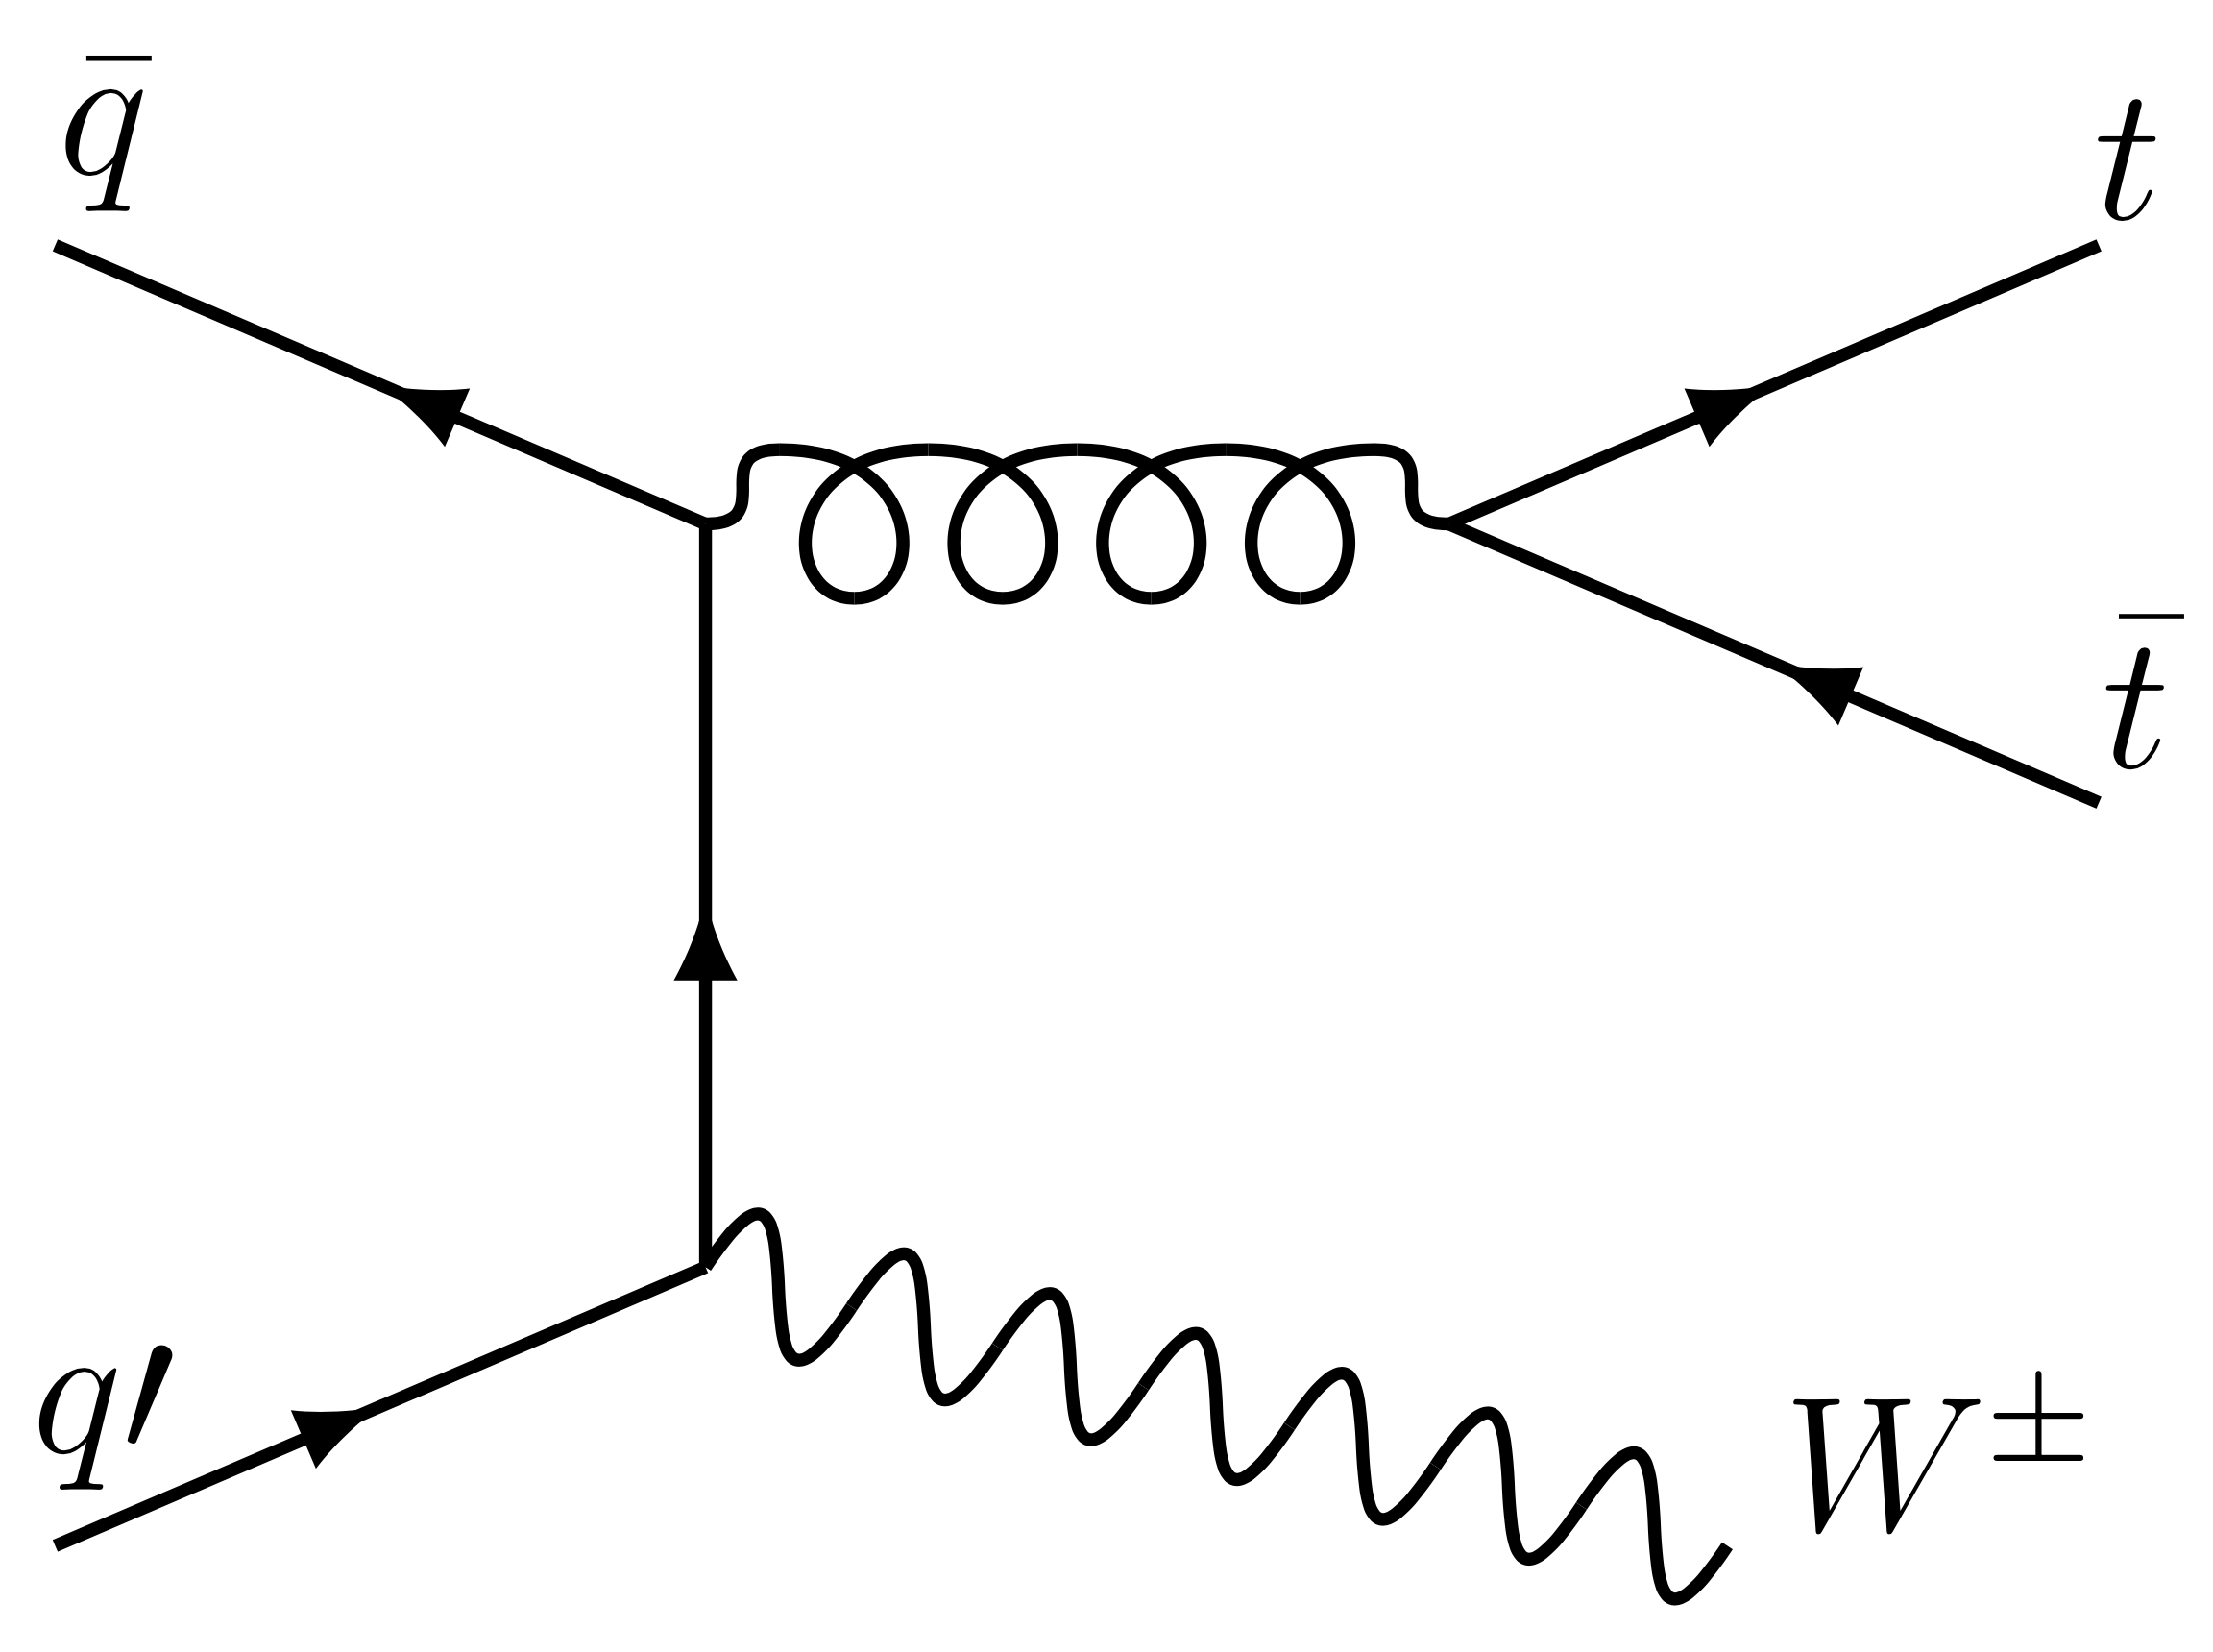
\includegraphics[width=\linewidth]{Chapter1/ttW_qq_A}
                \caption{}
                %\label{}
        \end{subfigure}%
        \begin{subfigure}[b]{0.25\textwidth}
                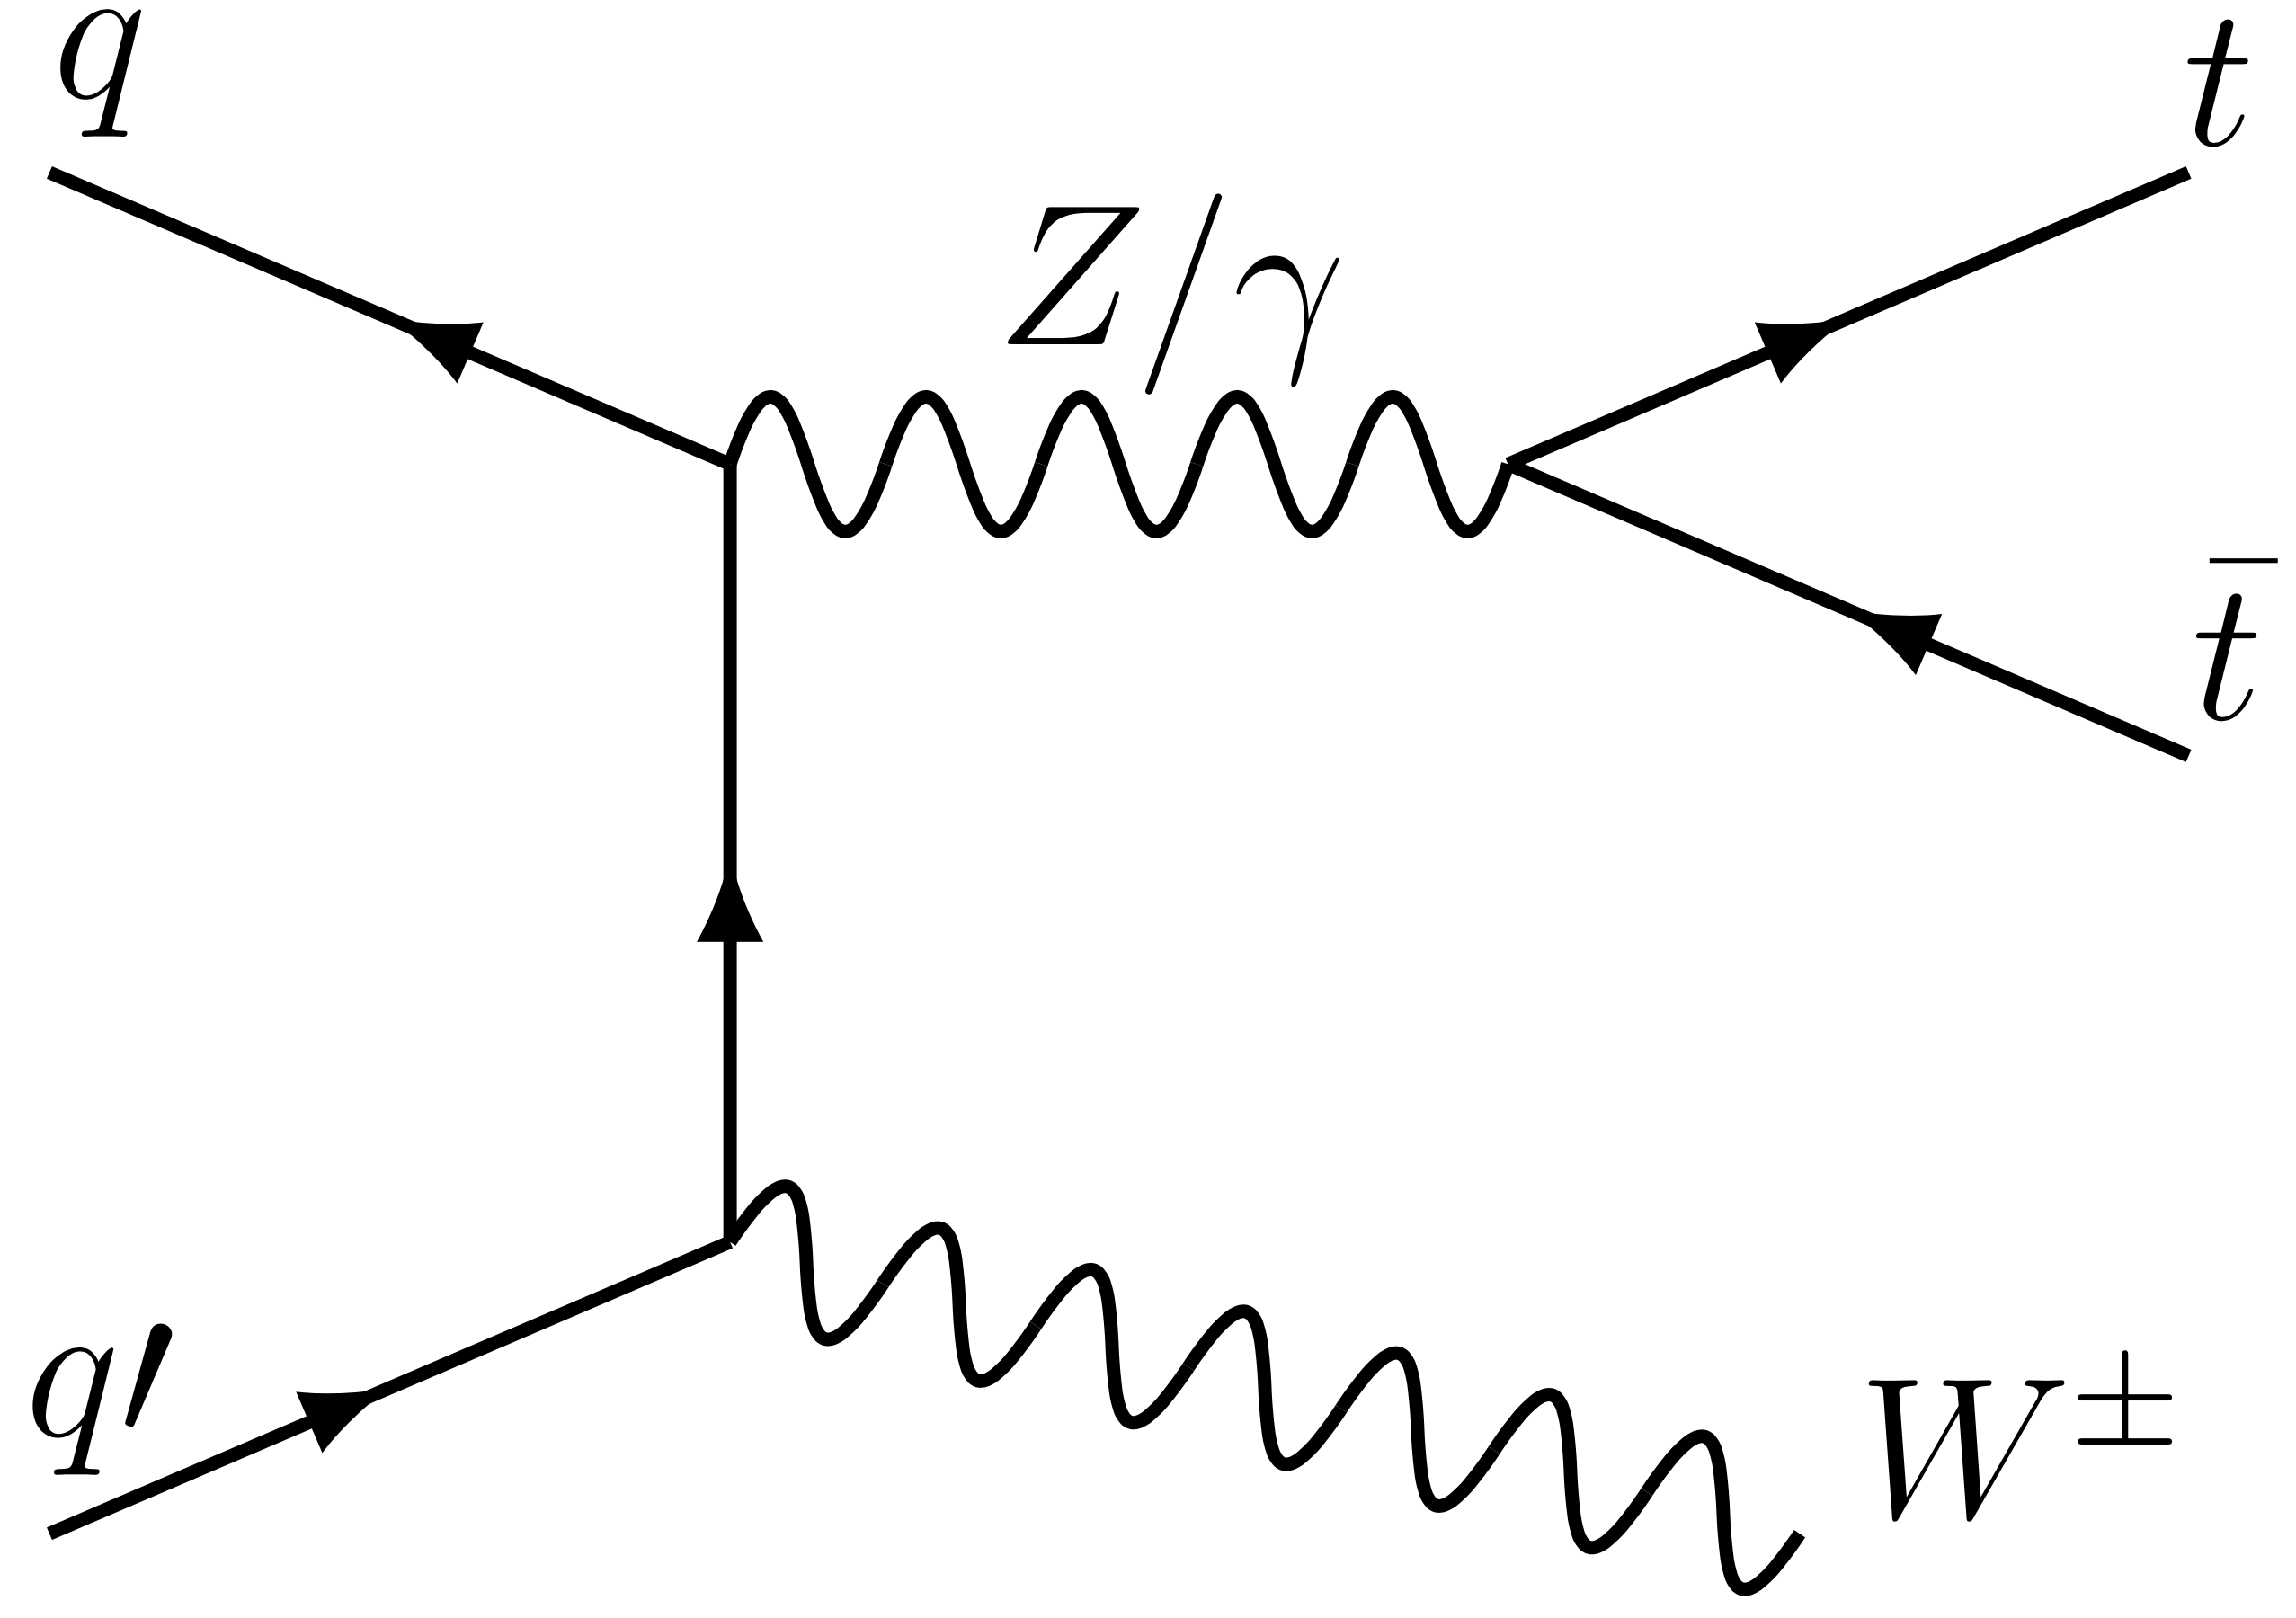
\includegraphics[width=\linewidth]{Chapter1/ttW_qq_B}
                \caption{}
                %\label{}
        \end{subfigure}%
        \begin{subfigure}[b]{0.25\textwidth}
                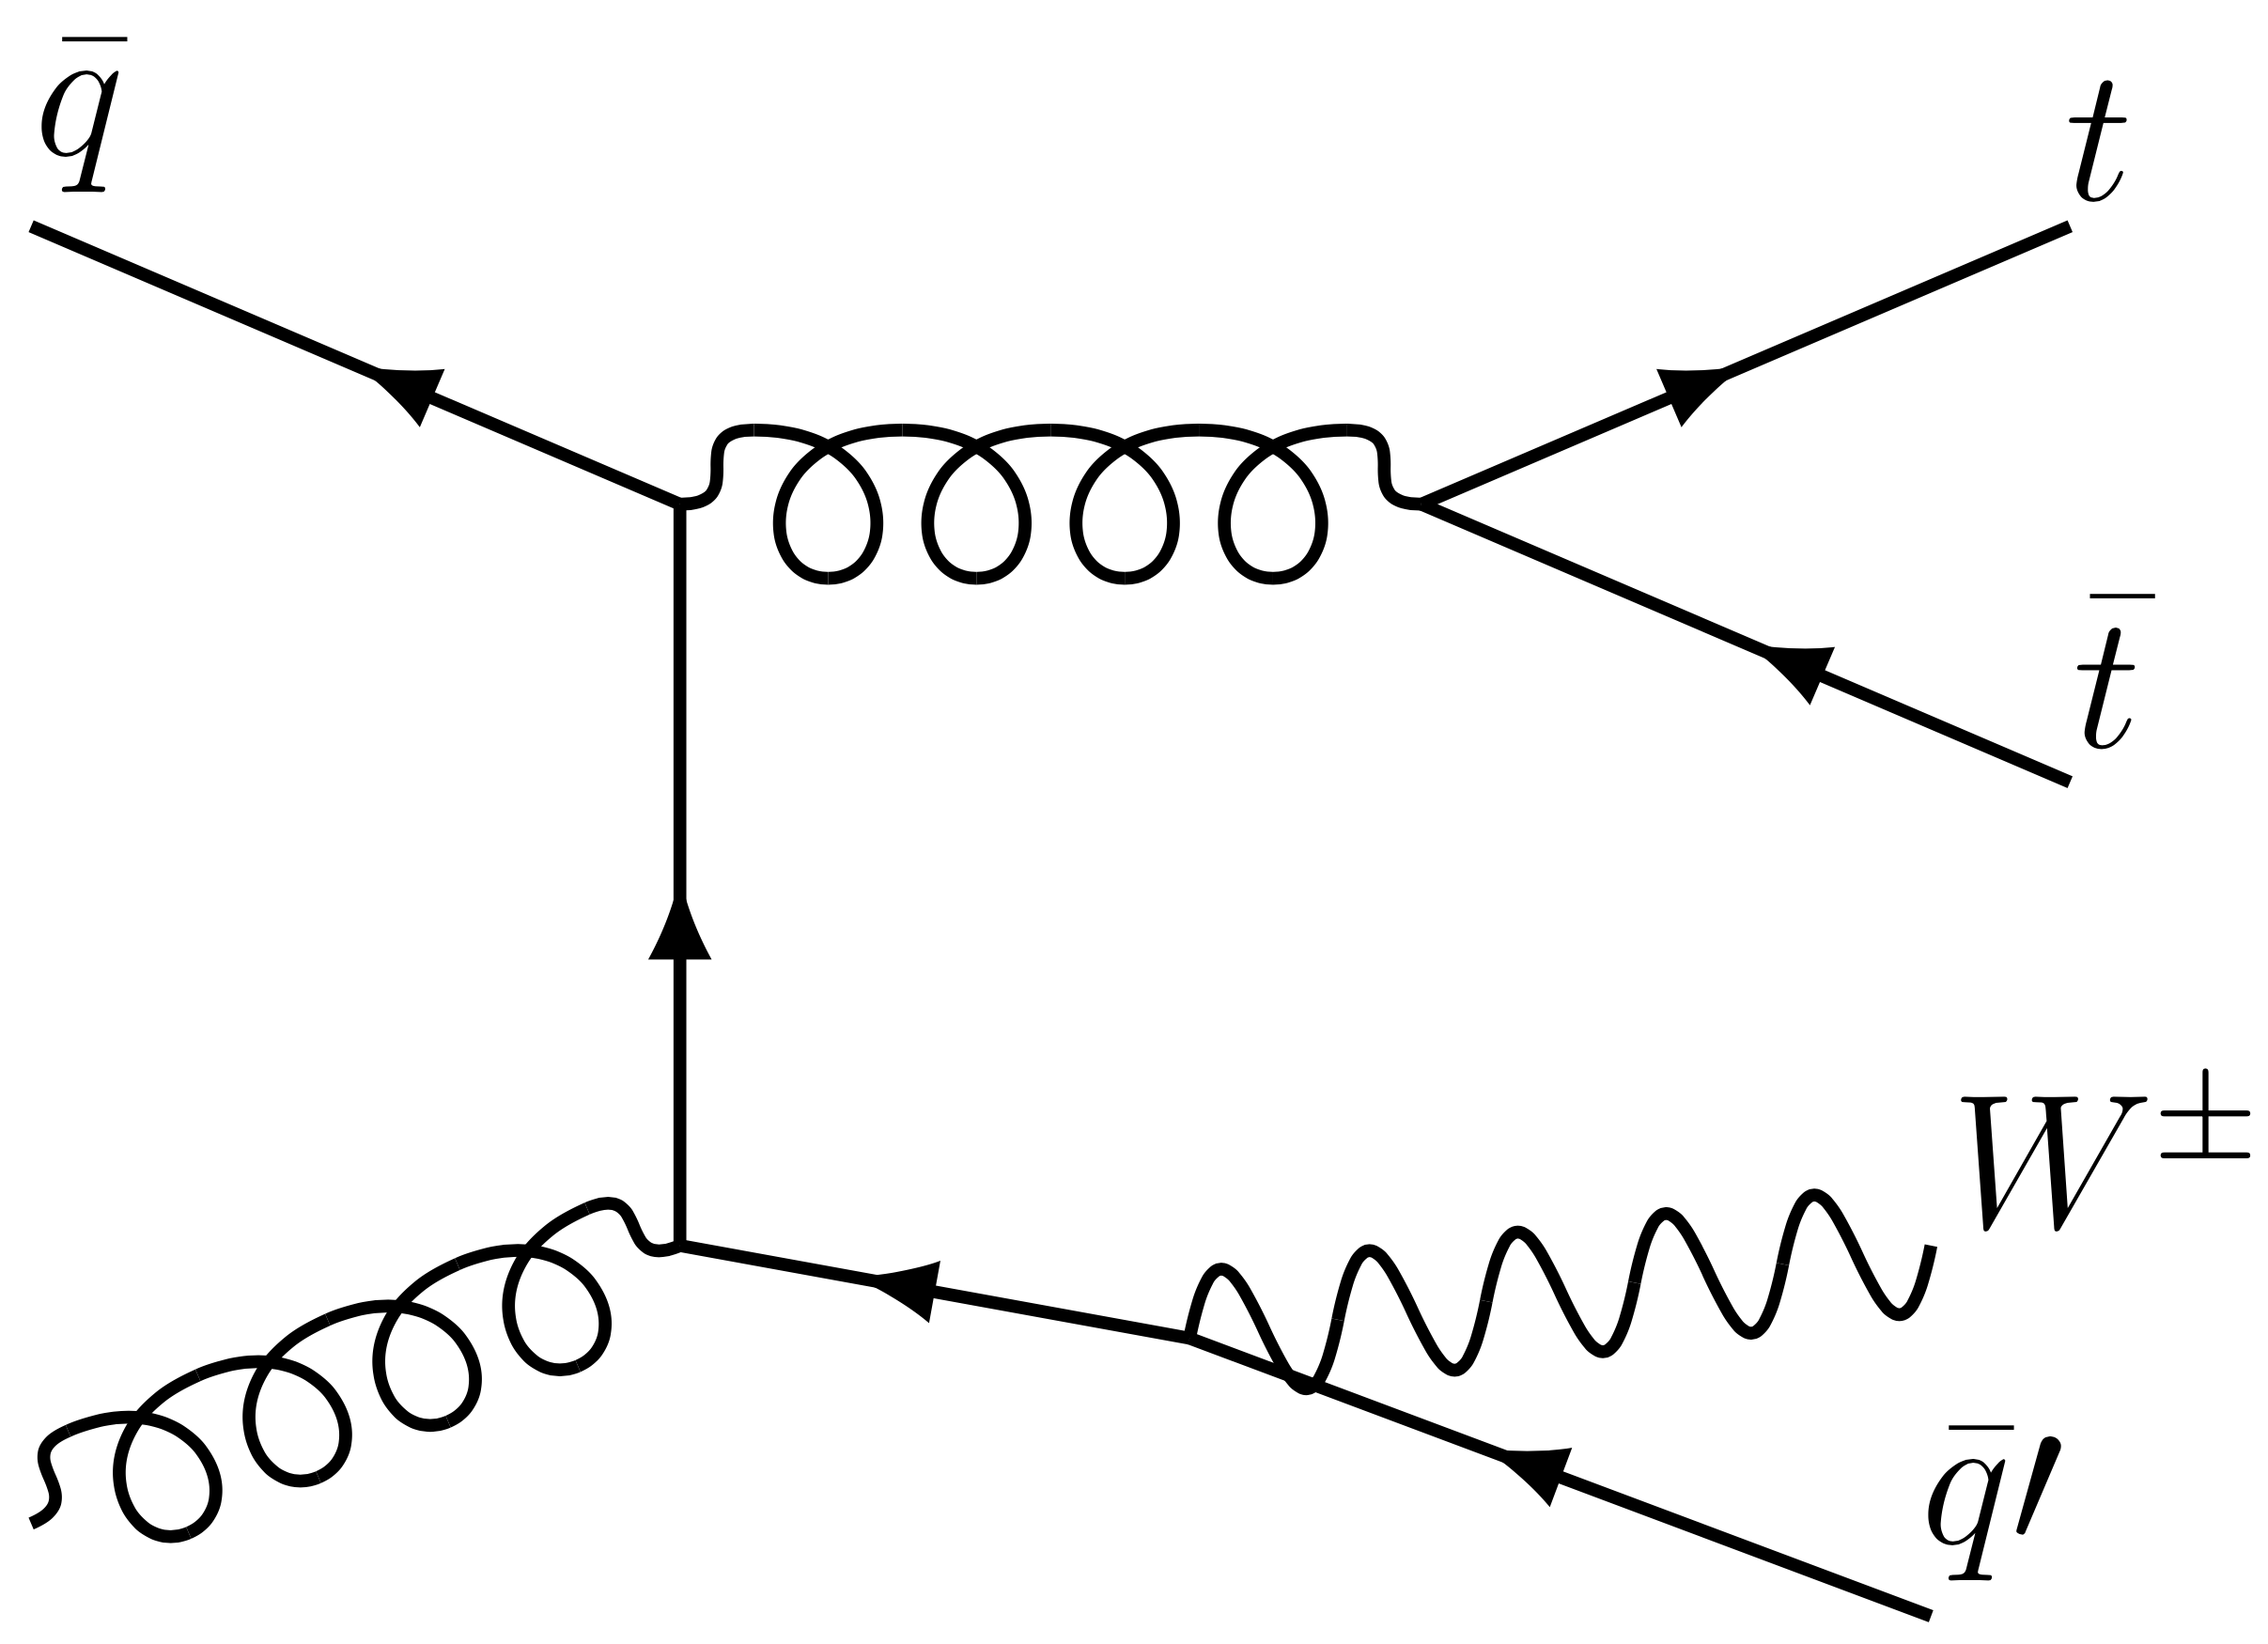
\includegraphics[width=\linewidth]{Chapter1/ttW_gq_A}
                \caption{}
                %\label{}
        \end{subfigure}%
        \begin{subfigure}[b]{0.25\textwidth}
                \includegraphics[width=\linewidth]{Chapter1/ttW_gq_B}
                \caption{}
                %\label{}
        \end{subfigure}
        \caption{Representative Feynman diagrams for \ttW production.
        Left diagrams show the $\bar{q}q'\rightarrow \ttW$ processes 
        and right ones the $\bar{q}g\rightarrow \ttW q'$ production. \pablo{igual tampoco
        	hace falta enseñar estos diagramas}}\label{fig:Chap1:top:ttX:ttW_Feynman}
\end{figure}
\end{comment}

The cross-sections for the \ttW, $\ttbar \gamma$ and $\ttbar \PZ$ productions 
are measured by the ATLAS and CMS collaborations. % with a large degree of agreement between the 
%two experiments. %The ATLAS measurements and NLO calculations for \ttW are 
%$\sigma_{\ttW} = 0.87 \pm 0.27\,\text{pb}$~\cite{ATLAS:2019fwo}, 
%$\sigma^{pred}_{\ttW} = 0.72^{+0.08}_{-0.09}\,\text{pb}$~\cite{ATLAS:2018fwq}. For the $\ttbar \gamma$
%process $\sigma_{\ttbar \gamma} = 0.798 \pm 0.055\,\text{pb}$~\cite{ATLAS:2020yrp}, 
%$\sigma^{pred}_{\ttbar \gamma} = 0.77\pm0.14\,\text{pb}$. The $\ttbar \PZ$ production yields
%a cross-section of $\sigma_{\ttbar \PZ} = 0.99 \pm 0.13\,\text{pb}$~\cite{ATLAS:2021fzm}, 
%$\sigma^{pred}_{\ttbar \PZ} = 0.86^{+0.09}_{-0.11}\,\text{pb}$~\cite{Kulesza:2020nfh}. 
These are presented in 
Figure~\ref{fig:Chap1:top:ttX:Cross-Sec}. For the three \ttX, the cross-sections
are small in comparison to \ttbar and single top-quark productions.
However, with the complete LHC Run 2 data event sample it is possible to explore these productions, which
are also sensitive to new physics~\cite{ATLAS:2020hpj}. 
The associated production of a \ttbar pair with a Higgs boson (\ttH) is another important
type of \ttX production and it is described in Section~\ref{sec:Chap1:ttH}.

\begin{figure}[h]
    \centering
    \includegraphics[width = 0.9\textwidth]{Chapter1/xsec_2023_ttX}
    \caption{Summary of the ATLAS and CMS measurements of the $\ttbar X$ production 
    cross-sections at $\CM =13$~TeV. Here $X$ means either $\PW$, $\PZ$ or $\Pgamma$.} %\pablo{Esta figura se queda porque ahorra tenxto.}} %Update from https://twiki.cern.ch/twiki/bin/view/LHCPhysics/LHCTopWGSummaryPlots#Pair_production_cross_section
    \label{fig:Chap1:top:ttX:Cross-Sec}
\end{figure}

%%%%%%%%%%%%%
%                tX              %
%%%%%%%%%%%%%
\subsubsection{Associated \tX production}
\label{sec:Chap1:Top:Production:top_plus_X}
Not only the top-quark pairs but also the single top quark can be produced
in association with other particles (\tX).
This thesis focusses precisely on the search of a \tX production, the
one in which the single top quark is produced along a Higgs boson and
an additional parton (\tHq). The features of the single-top-quark production 
in association with a Higgs boson are discussed in more detail in 
Section~\ref{sec:Chap1:tHq}.

Apart from being the signal process, the \tX production also plays a role
in the background since the \tZq process
is one of the backgrounds more difficult to separate from the \tHq signal. 
%in the final state characterised by two light-flavour leptons and one hadronic tau in the scenario in which
%the light leptons have a different electric charge (\dilepOStau).

%This type of production
%play an important role in the \tHq searches carried in this thesis since the \tZq process
% is one of the backgrounds more difficult to separate 
The other associated $\tX$ production of the EW type is the $\Ptop q \Pgamma$, in which the
top quark is produced along with a photon. Both \tZq and $\Ptop q \Pgamma$
are sensitive to beyond the SM (BSM) physics like flavour-changing neutral currents or vector-like quarks.
ATLAS and CMS have measured both processes and have found an agreement with the SM model, as 
as can be seen in  Figure~\ref{fig:Chap1:top:tX:Cross-Sec}.
%while for \tZq a good SM agreement
%is found, this is not the case for the $\Ptop q \Pgamma$ as can be seen in 
%Figure~\ref{fig:Chap1:top:tX:Cross-Sec}.

%In this work, the most relevant $\tX$ mode is the 
%single-top-quark production in association with a Higgs boson
%This is the main process to search for in the thesis and its features
%are discussed in more detail in Section~\ref{sec:Chap1:tHq}.

\begin{figure}
    \centering
    \includegraphics[width = 0.9\textwidth]{Chapter1/xsec_2023_tX.pdf}
    \caption{Summary of the ATLAS and CMS measurements of the $\tX$ production 
    cross-sections at $\CM =13$~TeV. Here, $X=\PZ$, $\Pgamma$ and \PW. The \tHq process 
    in not included in this summary plot but the work developed in this thesis aims to help
    to provide better limits on its cross-section.} %Update from https://twiki.cern.ch/twiki/bin/view/LHCPhysics/LHCTopWGSummaryPlots#Pair_production_cross_section
    \label{fig:Chap1:top:tX:Cross-Sec}
\end{figure}







%%%%%%%%%%%%%%%%%
%                Top decay               %
%%%%%%%%%%%%%%%%%
\subsection{Top-quark decay}
As anticipated in Section~\ref{sec:Chap1:Top:Production:SingleTop}, due to the large 
value of the $V_{tb}$ element of the CKM matrix, the 
top quark is expected to decay almost entirely ($\sim 99.8 \%$) %through the medium of the \Wtb vertex 
to a \Pbottom quark and a \PW boson ($\Ptop \rightarrow \PW \Pbottom$).
%The \tWb vertex and the decay chain of the top quark is 
%represented in Figure~\ref{fig:Chap1:top:decay:TopQuarkDecay}.
The final-state decay is classified according to the subsequent decay of the \PW boson.
Since the \PW bosons are massive vector bosons,
their lifetime is very short ($\tau_{\PW} \approx 3\times10^{-25}$~s) and hence they will
rapidly decay to leptons or quarks that will form hadrons. 
Due to its large mass, the \PW boson can decay to any quark except the top quark. 
For the \PWplus, the branching ratios\footnote{For each decay mode, the branching ratio (BR) is defined as the fraction times that the particle decays in that particular mode with respect to total possible decays.} (BRs) for the different decay modes are~\cite{Workman:2022ynf}:
\begin{align*}
	\PWplus &\rightarrow \Ppositron \Pneutrino_{e} 			&& (10.71 \pm 0.16)\%, \\
	\PWplus &\rightarrow \APmuon \Pneutrino_{\mu} 			&& (10.63 \pm 0.15)\%, \\
	\PWplus &\rightarrow \APtauon \Pneutrino_{\tau} 			&& (11.38 \pm 0.21)\%, \\
	\PWplus &\rightarrow \Pquark \APquark \textrm{ (hadrons)}	&& (67.41 \pm 0.27)\%, \\
	\PWplus &\rightarrow \textrm{invisible}					&& (1.4 \pm 2.9)\% .
\end{align*} 
For the conjugate proceses involving the \PWminus, the BRs are the same. Therefore, the \PW boson decay 
and consequently the top-quark decay can be classified either as leptonic or hadronic. 


%\begin{figure}
%    \centering
%    \includegraphics[width = 0.3\textwidth]{Chapter1/TopQuarkDecay}
%    \caption{Decay of a top quark to a \Pbottom quark and a \PW boson. The \PW boson can 
%    		decay either leptonically to a neutrino and a lepton
%    		or hadronically to a pair of light-flavour quarks. In the hadronic \PW decay, 
%		a jet triplet is formed along with the \Pbottom quark.}
%    \label{fig:Chap1:top:decay:TopQuarkDecay}
%\end{figure}







%%%%%%%%%%%%%%%%%%%%
%                Top polarisation               %. Not including polarisation in the thesis
%%%%%%%%%%%%%%%%%%%%
\subsection{Top-quark properties}
As commented, the top quark exhibits unique properties and plays a pivotal role in many analyses conducted at the LHC. 
Some of the key investigations related to the top quark are:

\begin{itemize}
	\item \textbf{Charge asymmetry in \ttbar production}: This refers to the subtle deviation observed between the rapidity distributions of top quarks and top antiquarks when produced in pairs~\cite{ATLAS:2022wec}.
	
	\item \textbf{Polarisation of \PW bosons in top-quark decays}: A measurement of the polarisation of the \PW bosons is conducted by quantifying the fractions of longitudinally, left-handed, and right-handed polarised \PW bosons~\cite{ATLAS:2022rms}.
	
	\item \textbf{Top--antitop-quark energy asymmetry}: Analogous to the charge asymmetry, this research focuses on scenarios where the top-quark pair is produced in association with a high-\pT jet~\cite{ATLAS:2021dqb}.
	
	\item \textbf{Top-quark-pair spin correlations}: Due to the  short lifetime of the top quark, its spin information can be extracted from its decay products. Nonetheless, not all decay particles carry the spin information equivalently.  Charged leptons emanating from leptonically decaying \PW bosons almost wholly encapsulate the spin information of the top quark~\cite{ATLAS:2019zrq}.
	
	\item \textbf{Flavour changing neutral currents (FCNCs):} A FCNC is a process where a quark 
	of one flavour changes into a quark of another flavour, without a change in its electric charge. 
	Top quarks, due to their large mass, are particularly interesting when it comes to FCNCs. 
	The top quark can decay through FCNC processes to lighter quarks in association with a photon, \PZ boson, or gluon.
	%Given that the Higgs boson possesses a smaller mass than the top quark, any emergence of 
	%FCNC would predominantly manifest during top-quark decay~\cite{ATLAS:2018jqi}.
	% FCNC are forbidden at tree level by the SM. This is due to the GIM mechanism.
	% However, FCNC can occur at higher orders
	
	\item \textbf{Top-quark polarisation}: In \tchannel single-top-quark production processes, there is a notable production of a highly-polarised-top quarks. These single top quarks manifest with spins completely aligned along the direction of the down-type quarks. Contrary, in the scenario of a single top antiquark, the alignment direction is inverted. A more comprehensive examination of polarisation can be found in Section~\ref{sec:Chap1:Top:Polarisation}, to which I have contributed during the tenure of this thesis. 
\end{itemize}%   Properties https://arxiv.org/pdf/1311.2028.pdf
%- 	mass
%- 	production and decay
%- 	electric charge
%- 	forward--backward asymmetry in \ttbar <- Only not SM observed
%- 	couplings to other SM particles


\subsubsection{Top-quark polarisation}
\label{sec:Chap1:Top:Polarisation}
% Polarisation paper: https://inspirehep.net/files/7e59402081847561840253401cf21138
% Figures from: https://atlas.web.cern.ch/Atlas/GROUPS/PHYSICS/PAPERS/TOPQ-2018-10/
% Presentation: https://indico.cern.ch/event/840542/contributions/3526240/attachments/1903250/3142485/LPCseminar_Negro.pdf
The lifetime of the top quark is shorter than the depolarisation scale
and, hence, the top-quark-spin information can be transferred into its decay products. This
allows to measure the top-quark polarisation from its child particles. The polarisation refers to 
the alignment between the momentum and the spin of the top quark and antiquarks.
The polarisations of the top and antitop quarks are important quantities because they are sensitive
to many BSM effects and can also provide useful input for the MC generators which are
described in Section~\ref{sec:Chap3.1:MC}.


At the LHC, the single-top-quark production is the only source of highly-polarised top quarks\footnote{The 
top quarks from the \ttbar production are unpolarised at LO but the spins of the top 
quarks and antiquarks are strongly correlated~\cite{CMS:2019nrx}.}. 
%   " The tops from ttbar are unpolarised at LO owing to the parity-conserving
%      nature (longitudinal polarization) and approximate time
%      invariance (transverse polarization) of QCD interactions."
In the \tchannel (see Section~\ref{sec:Chap1:Top:Production:SingleTop}) the top
quark is created with a high degree of polarisation in the direction of the spectator-quark momentum~\cite{ATLAS:2022vym}.
As a consequence of the vector and axial-vector
form of the coupling of the top quark to the \PW boson
and bottom quark in the \tchannel (\tWb vertex), specific
values of the polarisation vectors $\{P_{x'},\, P_{y'},\, P_{z'}\}$ of top
quarks/antiquarks are expected in the SM.

Even though it is not described in detail in this manuscript, during the development 
of my thesis I have also been involved in the first measurement of the top-(anti)quark-polarisation 
vectors~\cite{ATLAS:2022vym}. 
My contribution is an extension of the work done in Reference~\cite{Martinez-Agullo:2017lty}.
In this work, the three components of the polarisation 
vector for the top quark and antiquark are measured in the single-top-quark \tchannel production. Using the 
entire Run$\,$2 dataset recorded by ATLAS and demanding events with exactly one light lepton,
I defined a set of stringent selection requirements to discriminate the \tchannel signal 
from the background contributions. This signal-region\footnote{The signal region is a 
region of the phase space enriched with events of the signal process.}
definition used specific cuts\footnote{To ''cut´´ on a variable is to apply a threshold on this variable and
keep only events satisfying this condition. A cut-based analysis is
applying such thresholds on several variables to select events.}
 in several variables such as the lepton transverse momentum (\pT) or the invariant masses of several particles.
I have also developed the so called trapezoidal cut, which is described in the published 
paper~\cite{ATLAS:2022vym}.  

The polarisation vectors are later obtained from the distributions 
of the direction cosines of the charged-lepton momentum in the top-quark rest frame:
$\text{cos}(\theta_{lx'})$, $\text{cos}(\theta_{ly'})$ and $\text{cos}(\theta_{lz'})$. 
Figure~\ref{fig:Chap1:Polarisation:Observables} shows the distributions for one of these angular 
variables.

\begin{figure}[h]
\centering
	%\includegraphics[width=.3\textwidth]{Chapter1/PolarisationObservable_X}\hfill
	\includegraphics[width=.5\textwidth]{Chapter1/PolarisationObservable_Y}\hfill
	%\includegraphics[width=.3\textwidth]{Chapter1/PolarisationObservable_Z}
	\caption{Normalised differential cross-sections as a function of $\text{cos}(\theta_{ly'})$~\cite{ATLAS:2022vym}. 
	The data is shown as black points with statistical uncertainties compared to the 
	predictions of the MC generators, which are shown as lines. The ratio between the
	predictions and data is shown on the lower panel. 
	These plots are inclusive for top quark and top antiquark.} 
	\label{fig:Chap1:Polarisation:Observables}
\end{figure} 
%		We choose to show \text{cos}(\theta_{ly'}) instead
%		of \theta_{lx'} or \theta_{lz'} because it is related
%		to CP symmetry.

\begin{figure}[h]
    \centering
    \includegraphics[width=0.75\textwidth]{Chapter1/PolarisationFancy_PyPx}
    \caption{Observed best-fit limit on two-dimensional top quark polarisation
    parameter space $\{P_{x'},\, P_{y'}\}$. The statistical-only (green)
    and the statistical+systematic uncertainty contours have a 68\% CL~\cite{ATLAS:2022vym}.
    The physically allowed values for $P_{x'}$ and $P_{y'}$  lay inside the black circle. 
    The red point indicates the parton-level prediction at NNLO.}
    \label{fig:Chap1:Polarisation:Result}
\end{figure}


Limits on the two of the components of the polarisation vector of the
top quark and antiquark are set and Figure~\ref{fig:Chap1:Polarisation:Result}
presents the observed best-fit polarisation measurements for $P_{x'}$ and $P_{z'}$ in the
two dimensional parameter space.
%The components of polarisation are measured to be:
%\begin{minipage}[t]{0.45\textwidth}
%For top quarks
%	\begin{itemize}
%		\item $P_{x'}^{t} =  0.01 \pm 0.18$
%		\item $P_{y'}^{t} = -0.029 \pm 0.027$
%		\item $P_{z'}^{t} =   0.91 \pm 0.10$
%	\end{itemize}
%\end{minipage}
%\begin{minipage}[t]{0.45\textwidth} 
%For top antiquarks
%	\begin{itemize}
%		\item $P_{x'}^{\bar{t}} =  -0.02 \pm 0.20$
%		\item $P_{y'}^{\bar{t}} = -0.007 \pm 0.051$
%		\item $P_{z'}^{\bar{t}} =   -0.79 \pm 0.16$
%	\end{itemize}
%\end{minipage}

Data measurements of the polarisation-vector components and 
differential cross-sections show good agreement with SM predictions.
 The results are consistent with NNLO QCD predictions and expectation of
$P_{y'}^{t} = P_{y'}^{\bar{t}} = 0$ from the hypothesis of \CP symmetry 
in the top-quark and top-antiquark decay. 
%The significance of this analysis lies in the fact that within a relatively short 
%time period following the discovery of the top quark, it became feasible to 
%perform a differential measurement of its polarisation for the first time.





% The unfolding is performed with the TUnfold software package, developed at
% Deutsches Elektronen-Synchrotron (DESY). The process of unfolding can be thought
% of as correcting for blurring detector effects in order to unveil the spectrum of a given
% observable that is as close to the truth as possible.

%Angular measurements in ATLAS:
%\begin{itemize}
%	\item Top polarisation: how the top is produced
%	\item Helicity fractions: how the top decays
%	\item Spin correlation: information between produced top-quarks. 
%		Provides information about quantum entanglement. %source: https://indico.cern.ch/event/1139204/contributions/4850084/attachments/2437000/4174393/valencia_top.pdf
		
%\end{itemize} 


\begin{comment}
For polarisation:
Top polarised in direction of spectator quark
Define 3 Polarisation directions: $\{ P_{x´}, P_{xy}, P_{z´}, \}$
Lepton direction used as spin analyser ($\alpha_{l}$) 

In the single top \tchannel production, the top quark is polarised due to left-handed \PW-coupling.
Top-quark spin points in the direction of the spectator-quark(\Pq’) 


%%%%%%%%%%%%%%%%%%%%
%                   Top Physics                   %
%%%%%%%%%%%%%%%%%%%%
\subsection{Top quark physics}
\label{sec:Chap1:Top:Physics}
\pablo{Probably this section is not necessary since the physics are mostly explained above.}
The top quark couples directly to all SM vector (\Pphoton, \PWplus, \PWminus, \PZ, \Pgluon) 
and scalar (\PHiggs) bosons. For both photons and gluons, the interaction is 
described by a vectorial fermion-gauge coupling $\bar{\Psi}\Psi A_{\mu}$.
From boson-fermion interacting term of the $\mathcal{L}_{\text{QED}}$ in \ref{eq:chap1:QED_Complete}, the coupling 
of the top quark to photons (Figure~\ref{fig:Chap1:TopPhys:Couplings:A}) has a strength of 
$eQ\gamma^{\mu} =\frac{2}{3}e\gamma^{\mu}$. Meanwhile, for the top-gluon coupling (Figure~\ref{fig:Chap1:TopPhys:Couplings:g}),
the expanded form of the gluon-fermion term in the $\mathcal{L}_{\text{QCD}}$ of \ref{eq:chap1:QCD:Lagrangian_FinalCompact} gives the $g_{s}\frac{\lambda_{a}}{2}\gamma^{\mu}$.

\begin{figure}
\centering
\begin{subfigure}{.3\textwidth}
  \centering
  \includegraphics[width=.94\linewidth]{Chapter1/top_Coupling_topPhoton}
  \caption{Top-photon coupling.}
  \label{fig:Chap1:TopPhys:Couplings:A}
\end{subfigure}%
\begin{subfigure}{.3\textwidth}
  \centering
  \includegraphics[width=.94\linewidth]{Chapter1/top_Coupling_topGluon}
  \caption{Top-gluon coupling.}
  \label{fig:Chap1:TopPhys:Couplings:g}
\end{subfigure}
\begin{subfigure}{.3\textwidth}
  \centering
  \includegraphics[width=.94\linewidth]{Chapter1/top_Coupling_topWb}
  \caption{Top-\PW coupling.}
  \label{fig:Chap1:TopPhys:Couplings:W}
\end{subfigure}%
\begin{subfigure}{.3\textwidth}
  \centering
  \includegraphics[width=.94\linewidth]{Chapter1/top_Coupling_topZ}
  \caption{Top-\PZ cuopling.}
  \label{fig:Chap1:TopPhys:Couplings:Z}
\end{subfigure}
\begin{subfigure}{.3\textwidth}
  \centering
  \includegraphics[width=.94\linewidth]{Chapter1/top_Coupling_toph}
  \caption{Top-Higgs coupling.}
  \label{fig:Chap1:TopPhys:Couplings:H}
\end{subfigure}
\caption{Top quark coupling to SM bosons.}
\label{fig:Chap1:TopPhys:Couplings}
\end{figure}


For the charged weak current only the only the left-handed top couples to the \PWpm with coupling. This is done
via the \Wtb vertex with a strength of $g\gamma^{\mu}(1-\gamma^{5})V_{tb}$ (Figure
\ref{fig:Chap1:TopPhys:Couplings:W}). The value of $V_{tb}$ is given in Table~\ref{tab:Chap1:CKM}.
%This can be obtained from equation~\ref{eq:chap1:EW:CovariantDerivatice1} andf
% $\mathcal{L}_{\text{EW}}$ in \ref{eq:chap1:EW:FinalL} .
The top couples to the \PZ bosons (Figure~\ref{fig:Chap1:TopPhys:Couplings:Z})with unequal left and right-handed components, 
$\frac{ig}{2\textrm{cos}\,\theta_{W}}\gamma^{\mu}(v_{t}-a_{t}\gamma^{5})$. Being $v_{t} =1/2 -2Q_{t} \textrm{sin}^{2}\theta_{W}$ 
and $a_{t} = 1/2$.
Finally, for the Higgs boson (Figure~\ref{fig:Chap1:TopPhys:Couplings:H}), the top 
quark couples with a Yukawa type interaction $\bar{\Psi}\Psi \phi$ with a strength 
$\yt = \frac{\sqrt{2}\mtop}{v}$, as equation~\ref{eq:chap1:HiggsMechanism:YukawaCoupling} states. 
All of these couplings are flavour-conserving, with the exception of the charged-current
interaction with the \PW bosons. 

\end{comment}


%%%%%%%%%%%%%%%%%%%%%
%                      Higgs boson                   %
%%%%%%%%%%%%%%%%%%%%%
\section{The Higgs boson}
\label{sec:Chap1:HiggsBoson}
%Following the top quark, the Englert--Brout--Higgs--Guralnik--Hagen--Kibble--Higgs boson or, for simplicity, Higgs boson (\PH) or just Higgs
Following the top quark, the Higgs boson (\PH)
is the second most massive particle in the SM with a mass of
$\mH = 125.25 \pm 0.17$~GeV~\cite{Workman:2022ynf}. The value provided by Reference~\cite{Workman:2022ynf} is an average
of the ATLAS combined measurement ($\mH = 124.86 \pm 0.27$~GeV~\cite{ATLAS:2018tdk}) 
and the CMS results ($\mH = 125.46 \pm 0.16$~GeV~\cite{CMS:2020xrn}). %$\mH = 125.46 \pm 0.13$(stat)$\pm 0.10$(syst) GeV
%~\cite{pdgHiggs}
%\footnotesize{assuming statistical uncertainties only, the uncertainty of this result is only $\pm18\%$} 
The existence of the Higgs boson was theorised in 1964 by three independent groups~\cite{PhysRevLett.13.321, PhysRevLett.13.508, PhysRevLett.13.585}, and its discovery meant one of the greatest successes of the SM. 
%This theory was not only able to calculate with great precision the 
%observed physics phenomena but also predicted the existence of a particle 
%that was found later, as is described in Section~\ref{sec:Chap1:HiggsPhys_discovery}.

\begin{comment}
In the SM, fundamental particles acquire mass through their interactions with the Higgs fields. It is important to note that not all mass is related to the Higgs mechanism.
For instance, the mass of the proton does not came from the interaction of its components with the Higgs but from the kinetic energy of the particles that compose the proton.
\end{comment}

%%%%%%%%%%%%%%%%%%%%%
%                      Higgs discovery             % Maybe remove this
%%%%%%%%%%%%%%%%%%%%%
\subsection{Discovery of the Higgs boson}
\label{sec:Chap1:HiggsPhys_discovery}
Any particle physicist enthusiast remembers July 4th of 2012 pretty well, it was the day when 
the ATLAS~\cite{20121_ATLAS_HiggsDiscovery} 
and CMS~\cite{201230_CMS_HiggsDiscovery} collaborations
announced the discovery of a massive state \PH with the properties expected for the Higgs boson
within the SM.
%This discovery of the Higgs boson and, by extension, the Higgs field completed the SM.
% Was the Higgs boson found then the one predicted by Higgs and Englert or one of many?
% There is no theoretical predictions for the Higgs mass

Both the ATLAS and CMS collaborations reported excesses of events for 2011 (\CM=7 TeV and \lumi=4.8 fb$^{-1}$) 
and 2012 (\CM=8 TeV and \lumi=5.8 fb$^{-1}$) datasets of $\Pproton \Pproton$ collisions at the LHC.
This surplus of events was compatible with its production and decay with the SM Higgs boson in the
mass region $\mH \in [124$, $135]$~GeV. %with significances of 2.9$\sigma$ for ATLAS and 3.1 $\sigma$ for CMS.
Before that, the CDF~\cite{CDF:2012jmx} and D$\emptyset$
~\cite{D0:2012jgw} collaboration at Tevatron also reported
an excess in the mass region $\mH \in [120$, $135]$~GeV both of them with a 
significance lower than $3\sigma$ and therefore, not enough to clean a discovery\footnote{The 
$3\sigma$ expresses that there is a 99.7\% probability that a given result is not a 
random fluctuation, meaning there is roughly a 0.3\% chance that the observed 
effect is due to random chance. A 3$\sigma$ level is often considered evidence for a potential discovery.}.
% Tevatron = circular proton--antiproton collider at Fermilab



%%%%%%%%%%%%%%%%%%%%%%%%%
%                       Higgs production                       %
%%%%%%%%%%%%%%%%%%%%%%%%%
\subsection{Higgs-boson production at LHC}
%\paragraph{\PHiggs production}\mbox{}\\
\label{sec:Chap1:Higgs_production}

One of the reasons the Higgs boson was the last of the SM's fundamental particles to be discovered is 
its relatively high mass, which required significant energy for its production.
Even in high-energy collisions, the production of a Higgs boson is a rare event. Only a tiny fraction 
of collisions at the LHC produce a Higgs boson, so vast numbers of collisions had to be analysed to 
find the Higgs boson. This is the reason why it was not found at Tevatron.
% https://www.physicsforums.com/threads/why-was-higgs-not-discovered-at-tevatron.720104/
Colliders such as SLAC's Linear Collider~\cite{SLAC:design} or CERN's LEP~\cite{LEP:design} had enough energy
to produce the Higgs boson but 
they were colliding electrons and positrons.
Since the coupling of the Higgs boson to fermions is proportional to the fermion's mass, 
the $\Pelectron \APelectron \rightarrow \PHiggs$ process
is highly suppressed\footnote{The dominant Higgs-boson production in 
$\Pelectron \APelectron$ annihilation is the so called Higgsstrahlung, 
a process in which the $\PHiggs$ is produced in association 
with a $\PZ$ boson similarl to Figure~\ref{fig:Chap1:Higgs:LOFeynman_C}. Due to the 
small mass of the electrons, the electron--Higgs-boson coupling does not favour the 
$\Pelectron \APelectron \rightarrow \PHiggs$ process.} and, for this reason, 
there were not enough statistics of events with a Higgs boson at SLAC and LEP. The most favoured 
way of producing a Higgs boson is through the mediation of the heaviest 
fundamental particles in the SM because these have the strongest couplings 
with the Higgs boson and, consequently, the greater cross-sections.
%Figure~\ref{fig:Chap1:Higgs:LOFeynman} shows the dominant mechanisms for Higgs-boson production at the LHC. 
\begin{figure}[h]
\centering
\begin{subfigure}{.23\textwidth}
  \centering
  \includegraphics[width=.99\linewidth]{Chapter1/Higg_Production_LO_FeynmanDiagrams_gluonFusion}
  %\caption{Gluon Fusion\\ ($\Pgluon \Pgluon$F)}
  \caption{Gluon--gluon fusion}
  \label{fig:Chap1:Higgs:LOFeynman_A}
\end{subfigure}%
\begin{subfigure}{.23\textwidth}
  \centering
  \includegraphics[width=.99\linewidth]{Chapter1/Higg_Production_LO_FeynmanDiagrams_VectorBosonFusion}
  %\caption{\PW or \PZ fusion\\ (VBF)}
  \caption{Vector boson fusion}
  \label{fig:Chap1:Higgs:LOFeynman_B}
\end{subfigure}%
\begin{subfigure}{.23\textwidth}
  \centering
  \includegraphics[width=.99\linewidth]{Chapter1/Higg_Production_LO_FeynmanDiagrams_HiggstrahlungFusion}
  \caption{Higgsstrahlung}
  \label{fig:Chap1:Higgs:LOFeynman_C}
\end{subfigure}%
\begin{subfigure}{.23\textwidth}
  \centering
  \includegraphics[width=.99\linewidth]{Chapter1/Higg_Production_LO_FeynmanDiagrams_AssociatedttH}
  \caption{\ttH production}
  \label{fig:Chap1:Higgs:LOFeynman_D}
\end{subfigure}%
\caption{LO Feynman diagrams for the dominant production mechanisms of a Higgs boson at hadron colliders.}
\label{fig:Chap1:Higgs:LOFeynman}
% The strength of Higgs coupling to other particles depends on their mass and for this reason it likes to 
% accompany large mass produced particles like those containing the heaviest top quark
\end{figure}

The four most dominant processes for Higgs-boson production at LHC are 
summarised in Figure~\ref{fig:Chap1:Higgs:LOFeynman}. These processes are:
\begin{itemize}
  \item \textbf{Gluon--gluon Fusion} ($\Pgluon \Pgluon$F): 
				%This channel is depicted in Figure~\ref{fig:Chap1:Higgs:LOFeynman_A} and, as the diagram shows, 
				The process 
				$\Pgluon \Pgluon \rightarrow \PHiggs$ has to be mediated by a massive fermion loop. This is due to the fact that
				there is no direct gluon--Higgs-boson coupling within the SM.
				Although in principle all quarks should be included in the
				loop, in practice it is the top quark the one doing so because its coupling to the Higgs boson is 35 times stronger
				than the next-heaviest fermion, the bottom quark.
				Due to the abundance of gluons in $\Pproton \Pproton$ collisions, the $\Pgluon \Pgluon$F is very favoured at the LHC.
				
				%Another interesting property is that the $\Pgluon \Pgluon$F production rate is sensitive to the \CP-mixing angle in 
				%the top Yukawa coupling. %This is related to one of the major aims of this thesis, the search of a presence of
				%\CP-odd contributions in \yt.
				%This feature is related to that presented by the measurement of the \tHq production, the search for the presence of
				%\CP-odd contributions in \yt
				
							
  \item \textbf{Vector boson fusion} (VBF): 
  				The second most important mode is the radiation by the incoming quarks of a pair of
				\PW or \PZ bosons that fuse to 
  				form a Higgs boson. %as Figure~\ref{fig:Chap1:Higgs:LOFeynman_B} illustrates. 
				The vector bosons ($V=\PW$ or $\PZ$) of
				the process $V\bar{V}\rightarrow \PHiggs$ are originated from initial state quarks which scatter
				through the final state (changing its flavours in the case of \PW fusion) producing two forward jets.

  \item \textbf{Higgsstrahlung} (VH): 
  				There is another significant contribution involving the \PW or \PZ bosons, the Higgsstrahlung or associated 
				$\PW\PH$ or $\PZ\PH$ production. Here, an off-shell \PW or \PZ boson (formed from the annihilation of two 
				quarks) radiates a Higgs boson via $V^{*} \rightarrow V\PHiggs$. 
				%Figure~\ref{fig:Chap1:Higgs:LOFeynman_C} depicts the VH associated production.
				
  \item \textbf{Quark-pair associated production} ($q\bar{q}H$): 
  				In this mode, the Higgs is produced from a $q\bar{q}$ pair via $q\bar{q}\rightarrow \PHiggs$ with a $q\bar{q}H$
				final state. Typically, the involved quark pair is either a \bbbar or \ttbar. In the case of \ttbar, 
				the top quarks decay before hadronising, leading
				to final states with a high number of physics objects.
				
  \item \textbf{Single top quark associated production} ($tHX$): 
  				This sub-dominant contribution can be either a \tHq, a \tWH or a \schannel. The former 
				process constitutes the central topic 
				developed in this thesis. Details about these production modes are further
				discussed in Section~\ref{sec:Chap1:tHq}.
  
\end{itemize}
  



%Due to the abundance of gluons in $\Pproton \Pproton$ collisions, the most dominant one, i.e. the one with largest cross-section, 
%is the Higgs production via gluon fusion mediated by top quarks (Figure~\ref{fig:Chap1:Higgs:LOFeynman_A}). %This mode ($\Pgluon \Pgluon$F) 
%The second most important is the radiation by the incoming quarks of a \PW or \PZ vector bosons that fuse to 
%from a Higgs (Figure~\ref{fig:Chap1:Higgs:LOFeynman_B}). 
%There is another significant contribution involving the \PW or \PZ bosons, the Higgsstrahlung or associated 
%$\PW\PH$ or $\PZ\PH$ production, a process in which the \PW or \PZ (formed from the annihilation of two 
%quarks) radiate a Higgs boson(Figure~\ref{fig:Chap1:Higgs:LOFeynman_C}. 
%The last major contribution to the Higgs production at the LHC is its productions in association with a pair of 
%top and anti-top quarks (Figure~\ref{fig:Chap1:Higgs:LOFeynman_D}). 

The cross-section of the different mechanisms for single-Higgs-boson %\footnote{So far,
%the single Higgs production has been heavily studied at LHC but during Run\,3 the interest in double-Higgs production is increasing.}
production at $\CM=13$~TeV as a function of \mH are shown in Figure~\ref{fig:Chap1:Higgs:CrossSection}.
Assuming a $\mH=125.2$~GeV, the Higgs-boson production cross-sections ($\sigma_{\tH}$) for the different
modes (see relative fraction in Figure~\ref{fig:Chap1:Higgs:Prod_and_BR:Prod}) are~\cite{LHCHiggsCrossSectionWorkingGroup:2016ypw}:
%source: https://twiki.cern.ch/twiki/bin/view/LHCPhysics/CERNYellowReportPageAt13TeV

\begin{figure}[h]
\centering
\begin{subfigure}{.55\textwidth}
  \centering
  \includegraphics[width=.94\linewidth]{Chapter1/HiggsXSec_vs_mH_ZoomOut}
  \caption{}
  \label{fig:Chap1:Higgs:CrossSection:Out}
\end{subfigure}%
\begin{subfigure}{.45\textwidth}
  \centering
  \includegraphics[width=.94\linewidth]{Chapter1/HiggsXSec_vs_mH_ZoomIn}
  \caption{}
  \label{fig:Chap1:Higgs:CrossSection:In}
\end{subfigure}
\caption{Higgs-boson-production cross-sections as function of \mH 
at $\CM=13$~TeV~\cite{LHCHiggsCrossSectionWorkingGroup:2016ypw}.
The $\sigma_{\tH}$ presented in these plots accounts for the \tchannel and \schannel but not the $\Ptop\PW$ process.
A wide range of \mH values is showed in (a). In (b) is shown the result zooming 
around the measured Higgs-boson mass value.}
\label{fig:Chap1:Higgs:CrossSection}
\end{figure} % Source: Higgs boson CrossSection WG: https://twiki.cern.ch/twiki/bin/view/LHCPhysics/LHCHWG

\begin{minipage}[t]{0.3\textwidth}
  \centering\raisebox{\dimexpr \topskip-\height}{%
  \includegraphics[width=\textwidth]{Chapter1/Pie_HiggsXSec}}
  \captionof{figure}{Higgs-boson-production modes.}
  \label{fig:Chap1:Higgs:Prod_and_BR:Prod}
\end{minipage}\hfill
\begin{minipage}[t]{0.7\textwidth}
\begin{flushleft}
\begin{flalign*}
	\sigma_{\Pgluon \Pgluon\text{F}}	&= 48.5_{-3.3}^{+2.2}\,\textrm{pb} \\
	\sigma_{\text{VBF}}	&= 3.78 \pm 0.05\,\textrm{pb} \\
	\sigma_{WH} 	&= 1.37\pm 0.03\,\textrm{pb} \\
	\sigma_{ZH} 	&= 0.89^{+0.04}_{-0.03}\,\textrm{pb} \\
	\sigma_{\ttH}	&= 0.5^{+0.03}_{-0.05}\,\textrm{pb} \\
	\sigma_{\bbbar H}	&=0.49^{+0.10}_{-0.11}\,\textrm{pb} \\
	\sigma_{tHX}	&= 0.09\pm 0.01\,\textrm{pb} 
\end{flalign*}
\end{flushleft}
\end{minipage}



%%%%%%%%%%%%%%%%%%%%%%%%%
%                       Higgs decays                       %
%%%%%%%%%%%%%%%%%%%%%%%%%
\subsection{Higgs-boson decay}
%\paragraph{\PHiggs decay}\mbox{}\\
\label{sec:Chap1:Higgs_decay}

The Higgs boson has a very short lifetime ($\tau_{\PH} = 1.6 \times 10^{-22}$~s~\cite{LHCHiggsCrossSectionWorkingGroup:2016ypw}) and, hence,
is always detected through its decay products. 
%The branching ratio (BR) is the fraction of particles which decay by an individual decay mode with respect
%to the total number of particles which decay and for the Higgs is shown in Figure~\ref{fig:Chap1:Higgs:BR}.
Figure~\ref{fig:Chap1:Higgs:BR} shows the BR for the different Higgs-boson decay modes.
%\pablo{Looking at Figure~\ref{fig:Chap1:Higgs:BR:Out} it can be seen that if the Higgs weighted just about $50$~GeV more there would have been only two relevant decay modes, H->WW and H->ZZ.}

Despite the expected large Yukawa coupling between the 
Higgs boson and the top quark, the $\PH \rightarrow \ttbar$ is
forbidden since $\mH<2\mtop$. Consequently, the most 
prominent decay mode is $\PHiggs \rightarrow \bbbar$ followed by
$\PHiggs \rightarrow \PWplus \PWminus$. This is why for the \tHq searches, the 
channel in which the Higgs decay to \bbbar is the one with higher statistics. 
For the other fermionic decays, the decay rates are ordered by the fermion masses,
being the $\Ptauon\APtauon$ decay mode (see Figure~\ref{fig:Chap1:Higgs:DecayModes:Htautau}) 
the biggest among the leptonic ones. 
Regardless of the expected large coupling between the weak-force bosons and the Higgs boson, the $\PHiggs \rightarrow V V^{*}$ is
suppressed due to the requirement that one vector boson has to be produced off-shell\footnote{Off-shell means that the particle is produced virtually and it does not satisfy the energy--momentum relation: $E^2 = p^2 + m^2 $.}. 
%In the context of determining possible non-SM \CP contributions in the top-quark--Higgs-boson coupling, 
%the $\PHiggs \rightarrow \Pgamma \Pgamma$ is also a relevant process because this
%decay rate is sensitive to the Yukawa coupling of the top quark.



% The relevance of each production and decay mode is portrayed in the pie charts of Figure~\ref{fig:Chap1:Higgs:Prod_and_BR}. 
%Apart from the $\PWplus \PWminus$ decay, the other Higgs
%decay channel taken into consideration for the analysis carried in this thesis are $\PHiggs \rightarrow \PZ \PZ$ and $\PHiggs \rightarrow \Ptau \Ptau$.
For the analysis carried out in this thesis, three particular Higgs-boson-decay modes are considered: 
$\PHiggs \rightarrow \PWplus \PWminus$ (see Figure~\ref{fig:Chap1:Higgs:DecayModes:HWW}), $\PHiggs \rightarrow \PZ \PZ$ (see Figure~\ref{fig:Chap1:Higgs:DecayModes:HZZ}) 
and $\PHiggs \rightarrow \Ptauon \APtauon$ (see Figure~\ref{fig:Chap1:Higgs:DecayModes:Htautau}).
Sorted by its importance and assuming a $\mH=125.2$~GeV, the BRs for the Higgs boson  are presented in Figure~\ref{fig:Chap1:Higgs:Prod_and_BR:BR} and listed below~\cite{LHCHiggsCrossSectionWorkingGroup:2016ypw}. %~\cite{MelladoGarcia:2150771}: 
% Recommended values for SM Higgs BR: CERN Report4 :: https://cds.cern.ch/record/2150771/files/LHCHXSWG-DRAFT-INT-2016-008.pdf


\begin{minipage}[t]{0.35\textwidth}
\centering\raisebox{\dimexpr \topskip-\height}{%  
 \includegraphics[width=0.95\textwidth]{Chapter1/Pie_HiggsDecay}}
  \captionof{figure}{Higgs-boson-decay modes.}
  \label{fig:Chap1:Higgs:Prod_and_BR:BR}
\end{minipage}\hfill
\begin{minipage}[t]{0.45\textwidth}
\begin{flushleft}
\begin{flalign*}
	\PHiggs &\rightarrow  \bbbar 			& (57.92 \pm 0.29)\% \\
	\PHiggs &\rightarrow  \PWplus\PWminus	& (21.70 \pm 0.11)\% \\
	\PHiggs &\rightarrow  \Pgluon \Pgluon 	& (8.17 \pm 0.26)\% \\ 
	\PHiggs &\rightarrow  \Ptauon\APtauon	& (6.24 \pm 0.03)\% \\
	\PHiggs &\rightarrow  \Pcharm \APcharm	& (2.888 \pm 0.014)\% \\ 
	\PHiggs &\rightarrow  \PZ\PZ			& (2.667 \pm 0.013)\% \\
	\PHiggs &\rightarrow  \Pgamma \Pgamma	& (2.270 \pm 0.023)\% \\
	\PHiggs &\rightarrow  \Pmuon\APmuon	& (2.165 \pm 0.011)\% \\
	\PHiggs &\rightarrow  \PZ \Pgamma		& (0.155 \pm 0.008)\% \\
	\PHiggs &\rightarrow \text{Others}		& < 0.2 \%
\end{flalign*}
\end{flushleft}
\end{minipage}


\begin{figure}[h]
\centering
\begin{subfigure}{.5\textwidth}
  \centering
  \includegraphics[width=.94\linewidth]{Chapter1/HiggsBR_ZoomOut}
  \caption{}
  \label{fig:Chap1:Higgs:BR:Out}
\end{subfigure}%
\begin{subfigure}{.5\textwidth}
  \centering
  \includegraphics[width=.94\linewidth]{Chapter1/HiggsBR_ZoomIn}
  \caption{}
  \label{fig:Chap1:Higgs:BR:In}
\end{subfigure}
\caption{SM Higgs-boson-decay branching ratios as a function of \mH at $\CM=13$~TeV~\cite{LHCHiggsCrossSectionWorkingGroup:2016ypw}. In (a) the BRs are shown in a Higgs-boson mass 
range $\mH \in (90, 10^3)$~ GeV. In (b) only values of \mH around the measured one are shown.
 Looking at (a) it can be seen that if the Higgs boson
weighted just about $60$~GeV more there would have been only two relevant decay 
modes, \HWW and \HZZ. On the other hand, if Higgs had been just $20$~GeV lighter, these
two channels would have been very difficult to observe.}
\label{fig:Chap1:Higgs:BR}
\end{figure} % Source: Higgs boson CrossSection WG: https://twiki.cern.ch/twiki/bin/view/LHCPhysics/LHCHWG

\begin{figure}[h]
\centering
\begin{subfigure}{.25\textwidth}
  \centering
  \includegraphics[width=.75\linewidth]{Feynman_diagrams/H__WW}
  \caption{\HWW decay.}
  \label{fig:Chap1:Higgs:DecayModes:HWW}
\end{subfigure}%
\begin{subfigure}{.34\textwidth}
  \centering
  \includegraphics[width=.95\linewidth]{Chapter1/H_decayModes_Htautau}
  \caption{\Htautau decay.}
  \label{fig:Chap1:Higgs:DecayModes:Htautau}
\end{subfigure}%
\begin{subfigure}{.32\textwidth}
  \centering
  \includegraphics[width=.89\linewidth]{Chapter1/H_decayModes_HZZ}
  \caption{\HZZ decay.}
  \label{fig:Chap1:Higgs:DecayModes:HZZ}
\end{subfigure}
\caption{Representative LO Feynman diagrams for the Higgs-boson decay into a pair of (a) \PW bosons
(b) tau leptons and (c) \PZ bosons. 
The three decay modes are taken into account for the associated \tHq production described in this thesis.
In (b), the \APtauon is decaying to quarks which form hadrons, 
therefore, it is referred to as hadronic tau. In contrast, the \Ptauon in (b) is a leptonically-decaying tau. 
For the diagram in (c), the Higgs boson decays into a four light-flavoured-leptons final state.}
\label{fig:Chap1:Higgs:DecayModes}
\end{figure}

%\begin{figure}
%\centering
%\begin{subfigure}{.5\textwidth}
%  \centering
%  \includegraphics[width=.94\linewidth]{Chapter1/Pie_HiggsXSec}
%  \caption{Production}
%  \label{fig:Chap1:Higgs:Prod_and_BR:Prod}
%\end{subfigure}%
%\begin{subfigure}{.5\textwidth}
%  \centering
%  \includegraphics[width=.97\linewidth]{Chapter1/Pie_HiggsDecay}
%  \caption{Decay}
%  \label{fig:Chap1:Higgs:Prod_and_BR:BR}
%\end{subfigure}
%\caption{Percentage fractions for Higgs boson (a) production at $\CM=13$~TeV for $\Pproton \Pproton$ collisions and (b) BR fraction for different decay channels~\cite{LHCHiggsCrossSectionWorkingGroup:2016ypw}.}
%\label{fig:Chap1:Higgs:Prod_and_BR}
%\end{figure} % Source: https://cds.cern.ch/record/2800522?ln=en


\begin{comment}
%%%%%%%%%%%%%%%%%%%%%
%            Higgs boson physics                %
%%%%%%%%%%%%%%%%%%%%%
\subsection{Higgs boson physics}

\pablo{Work in progress}


The gauge symmetry is broken is broken by the vacuum, triggering the EW Spontaneous Symmetry Breaking (SSB). This means that the
symmetry group of the EW sector, $U(2)_\text{L} \bigotimes U(1)_\text{Y}$.

$SU(3)_\text{C} \bigotimes SU(2)_\text{L}} \bigotimes U(1)_\text{Y} \xrightarrow{\text{SSB}} SU(3)_\text{C}} \bigotimes U(1)_{\text{QED}}$ 

% Higgs boson mass and width. Coupling to bosons. Coupling to fermions https://inspirehep.net/files/6c0b1f30a286a7aca715341b4fd90442

Production and decay rates, constrains on its couplings: \url{https://arxiv.org/abs/1606.02266}

The Higgs mass is given by $\mH =\sqrt{\lambda /2} v $, being $v$ the vacuum expectation value of the Higgs field and $\lambda$ the Higgs self-coupling. 
%~\cite{Pich:2015lkh}

Electro weak symmetry breaking~\cite{Salam:1968rm}: \url{https://arxiv.org/pdf/1512.08749.pdf}
In this paper the Yukawa coupling of the top is introduced, link it with the tHq paper. 

% At peak lumi, the LHC was producing a $\PHiggs \rightarrow \Pgamma \Pgamma$ every 45 minutes~\cite hoecker

% Slide 34, BR of Higgs decays https://indico.cern.ch/event/763013/contributions/3358697/attachments/1813182/2962418/Higgs-1.pdf

\pablo{Work in progress}

\pablo{This is not getting into the thesis because we don't want to verbose that much but we could talk about: Lepton Flavour Violating (FLV) Higgs, dark Higgs, etc, etc}\pablo{The precision measurement of the properties of the Higgs is one of the main focusses of LHC.}

\end{comment}



%                          %
%  i n t e r p l a y  %
%                          %

\FloatBarrier

%%%%%%%%%%%%%%%%%%%%%
%                Top-Higgs interplay              %
%%%%%%%%%%%%%%%%%%%%%
\section{The interplay between the top quark and the Higgs boson}
\label{sec:Chap1:top-Higgs}

%General yt
The couplings of the Higgs boson to the SM particles are found to be 
uniquely determined by the masses of these particles. Being this strength proportional
to the mass in the case of fermions and the squared mass for the bosons. 
Figure~\ref{fig:Chap2:HiggsAllCouplings} presents 
the coupling--mass relationship of the Higgs boson with other SM particles.
Since the top quark is the most massive particle, 
the Yukawa coupling between the top quark and the Higgs boson, \yt is expected 
to be the strongest among all fermions and, hence, its
study is of crucial importance, as it is discussed in References~\cite{Farina:2012xp, Biswas:2012bd} 
and developed in the succeeding sections. The Yukawa coupling is expected to be of the order of the unity:
\begin{equation*}
	\yt = \frac{\sqrt{2}\mtop}{v} = 2^{3/4}G_{F}^{1/2}\mtop = 0.995 \simeq 1 \, .
\end{equation*}
This value is larger than the value of the couplings of the other quarks. For comparison
$y_b \simeq 0.025$ and $y_c \simeq 0.007 \gg y_{s,d,u}$. 

\begin{figure}
    \centering
    \includegraphics[width = 0.6\textwidth]{Chapter1/HiggsAllCouplings_Extended}
    \caption{Best fit values of the coupling of the Higgs boson to fermions (\Pmu, \Ptau, \Pbottom, \Ptop) 
    		and bosons (\PW, \PZ) as a function of the mass of the particles~\cite{ATLAS-CONF-2021-053, ATLAS-CONF-2015-007}. 
		% Scaled under some theoretical assumptions. ~\cite{Collaboration:2045852}
		The dotted line indicates the SM prediction and the uncertainty bars represent
		68\% confidence level (CL) intervals for the measured parameters. For the $\kappa_{\Pmu}$, the
		light uncertainty bars indicate a 95\% CL interval. The lower panel shows the ratio between the measured
		values and their SM predictions.}
    \label{fig:Chap2:HiggsAllCouplings}
\end{figure}


%   Yukawa coupling measurement
%   The SM expectation of the Yukawa coupling value is $\yt = \frac{\sqrt{2}\mtop}{v}$ = 0.9956 \pm 0.0043$ 
%   source :: https://iopscience.iop.org/article/10.1088/1361-6471/44/6/063001/pdf

%The study of the couplings of the Higgs to the other particles are of prime importance 
%since they control the behaviour of the whole theory at high energy
%"""
%Measuring processes involving real top quarks in the final state
%will bring invaluable information. With the largest rate, the Higgs production in association
%with a top pair is a golden channel and has received great attention by the experimental 
%as well as theoretical communities~\cite{Farina:2012xp}
%"""

%ttH
The production of a pair of top quarks along with a Higgs boson (\ttH) allows 
to measure the absolute value of \yt. This process has the advantage of 
being the leading mechanism to produce the Higgs together with the quark 
top. % At $\CM=13$~TeV it has a cross-section of \pablo{poner cálculos del SM para $\sigma_{\ttH}$}.
Section~\ref{sec:Chap1:ttH} discusses the \ttH production.

%tH
Having a much lower cross-section than \ttH, 
the Higgs-boson production alongside a single top quark (\tH) brings valuable information, especially
regarding the sign of the Yukawa coupling. Note that the sign of the Yukawa coupling is not a physical 
property by itself, but the relative sign compared to the coupling of the Higgs boson to 
gauge bosons\footnote{The coupling of the Higgs boson to the gauge bosons is taken as positive.} is indeed physical~\cite{Farina:2012xp}. 
This production mechanism is discussed in more detail in Section~\ref{sec:Chap1:tHq}. 

% "The sign of the top Yukawa coupling is not physical by itself, but the relative sign compared to the Higgs
%    coupling to gauge bosons (we take the latter to be positive) is physical." 
%									- Farina

%A change in the Yukawa sign and/or absolute value with respect to its SM value
%would signal an origin of the fermion masses different from the described by the EWSB
%because the relative sign of the Higgs coupling to fermions
%and gauge vector bosons is crucial for recovering the unitarity and renormalisability of the
%theory~\cite{Appelquist:1987cf}. \pablo{no estoy seguro de si este párrafo es cierto}





%%%%%%%%%%%%%%%%%%%%%%%
%                     CP in top-Higgs                     %
%%%%%%%%%%%%%%%%%%%%%%%
\subsection{\CP properties in top-quark--Higgs-boson interactions}
The \CP properties of the Yukawa coupling of the Higgs boson to the
top quark can be probed through the associated production of these 
two particles. While SM predicts the Higgs boson to be a scalar boson ($J^{\CP}=0^{++}$),
the presence of a $J^{\CP}=0^{+-}$ pseudoscalar admixture has not 
been excluded yet. This pseudoscalar would introduce a second coupling
to the top quark. Finding a \CP-odd contribution would be a sign of physics
beyond the SM and could account for the imbalance between matter and
antimatter in the universe~\cite{ATLAS:2020ior}. 

% A pseudoscalar is a quantity that behaves like a scalar, except that it changes sign under a parity inversion
% J = Spin
% C = charge conjugation eigenvalue
% P = Parity eigenvalue

The production rates of \ttH and \tH depend on the \yt coupling. The latter
is especially sensitive to \yt deviations from the SM as it is described in Section
\ref{sec:Chap1:tHq}. As already mentioned, the presence of a \CP-mixing in \yt would also affect the
$\Pgluon \Pgluon$F production and $\PHiggs \rightarrow \Pgamma \Pgamma$ decay rates.
As it is explained in Section~\ref{sec:chap1:SM_problems}, the existence of \CP violation is
one of the conditions needed to explain the matter-antimatter asymmetry~\cite{Sakharov:1967dj}.
%H-> gama gamma en https://arxiv.org/pdf/2004.04545.pdf
%ggF en https://arxiv.org/pdf/hep-ph/9303216.pdf



%%%%%%%%%%%%%%%
%              ttH                      %
%%%%%%%%%%%%%%%
\subsection{The \ttH process}
\label{sec:Chap1:ttH}
% ttH ATLAS (2019): https://atlas.web.cern.ch/Atlas/GROUPS/PHYSICS/CONFNOTES/ATLAS-CONF-2019-045/
% ttH CMS (2020): https://cds.cern.ch/record/2725523/files/HIG-19-008-pas.pdf
The production of \ttbar in association with a Higgs boson is one of the most important process
to measure the strength of the Yukawa coupling ($|\yt|$), which is crucial to understanding the origin of the fermion masses.
Detecting a deviation from the SM prediction for $\sigma(\ttH)$ could indicate the presence of new physics that
violates the \CP symmetry. But, as Figure~\ref{fig:Chap1:xsec_vs_yt_tH_ttH} illustrates, the  $\sigma(\ttH)$ has
a non-injective dependence with the Yukawa mixing angle.


From the phenomenology point of view, the calculations for the \ttH production cross-section
at $\CM=13$~TeV can be calculated an next-to-leading order
(NLO)$\,$+$\,$NNLL
accuracy~\cite{Broggio:2016lfj}:
\begin{equation*}
	\sigma_{\text{NLO+NNLL}}^{\text{pred}} (\ttH) = 486.4^{+29.9}_{-24.5}\,\text{fb}.
\end{equation*}
This calculation depends on the chosen scales for the soft and hard processes but it gives an idea of the order 
of magnitude for this process. The uncertainties are estimated through variations of the factorisation and
renormalisation scales.
%The LO Feynman diagrams for the \ttH production are presented in Figure~\ref{fig:Chap1:ttH:Feynman}. 
This process constitutes a relevant background in the analysis. % especially in the \dilepSStau channel
%where \ttH is the second largest background. %\pablo{revisar en el futuro esto del "2nd largest bkg", no sea que cambie algún yield.}
% https://inspirehep.net/literature/1495438

\begin{comment}
\begin{figure}
\centering
\begin{subfigure}{.45\textwidth}
  \centering
  \includegraphics[width=.9\linewidth]{Chapter1/ttH_Feynman_A}
  \caption{}
  \label{fig:Chap1:ttH:Feynman:A}
\end{subfigure}%
\begin{subfigure}{.45\textwidth}
  \centering
  \includegraphics[width=.9\linewidth]{Chapter1/ttH_Feynman_B}
  \caption{}
  \label{fig:Chap1:ttH:tFeynman:B}
\end{subfigure}%
\caption{LO Feynman diagrams for \ttH production. Although this is the most 
relevant mechanism for the associated production of a Higgs boson with, at least, one top quark, 
the \ttH is still a rare process. 
The \ttH accounts for roughly 1\% of all Higgs-boson production and it cross-section is a factor 100 
smaller than the $\Pgluon\Pgluon\text{F}$, as can be seen in Figure~\ref{fig:Chap1:Higgs:CrossSection:In}.}
\label{fig:Chap1:ttH:Feynman}
\end{figure}
\end{comment}


The first associated production of a Higgs boson with a pair of top 
quarks was observed in 2018 by ATLAS~\cite{ATLAS:2018mme} 
%with a signal strength $\mu=\sigma/\sigma_{SM} $ of $0.84^{+0.64}_{-0.61}$
and CMS~\cite{CMS:2018uxb} collaborations. %~\cite{Skovpen:2018aoe}
This process marked a significant milestone for the field of high-energy 
physics because it helped establish the first direct 
measurement of the tree-level coupling of the Higgs boson 
to the top quark, which is in agreement with the SM expectation.

%The associated production of Higgs boson with top quark pair 
The \ttH process has been studied by ATLAS and CMS previously
not only with Run$\,$1 dataset at $\CM=7$~TeV and $8$~TeV~\cite{ATLAS:2014ayi, CMS:2014tll} 
but also with Run$\,$2 dataset at $\CM=13$~TeV~\cite{ATLAS:2018mme, CMS:2018uxb}, where the cross-section was expected 
to be increased by a factor of four. 

The ATLAS combined measurement for the \ttH process using $79.8\,\text{fb}^{-1}$
and considering \bbbar, $\PWplus \PWminus$, \Ptauon\APtauon, \Pgamma\Pgamma and \PZ\PZ
Higgs-boson decay channels present the signal strength~\cite{ATLAS:2018mme}:
\begin{equation*}
	\mu_{\ttH} = \frac{\sigma(\ttH)}{\sigma^{SM}(\ttH)} = 1.32 \pm 0.13\,(\text{stat.})\, ^{+0.17} _{-0.15} (\text{syst.})\, .
\end{equation*}

For CMS, the \ttH signal strength has been measured
with a dataset corresponding to a luminosity of $137\,\text{fb}^{1}$
at $\CM=13\,$TeV.
For the $\gamma$$\gamma$ Higgs-boson-decay 
channel~\cite{CMS:2020cga}
\begin{equation*}
	\mu^{\Pgamma \Pgamma}_{\ttH} = 1.14^{+0.36} _{-0.29}
\end{equation*}
and for the $\PWplus$$\PWminus$, $\Ptauon$$\APtauon$, $\Pgamma$$\Pgamma$ and $\PZ$$\PZ$ Higgs-boson-decay channels
with multileptonic final states~\cite{CMS-PAS-HIG-19-008}
\begin{equation*}
	\mu^{\text{MultiLep.}}_{\ttH} = 0.92 \pm 0.19\,(\text{stat.})\, ^{+0.17} _{-0.13} (\text{syst.})\, .
\end{equation*}
%\begin{equation*}
%	\mu_{\ttH} = 1.14 \pm 0.18(\text{stat.}) ^{+0.21} _{-0.19} (\text{syst.})
%\end{equation*}
%final states with hadronic taus not included in the CMS combination
As can be seen, the statistical uncertainty of these results is sometimes dominating 
the measurements. Therefore, an analysis with more data would be very beneficial
to have more precise results.

%The ATLAS Run$\,$2 analyses use an integrated 
%luminosity up to 79.8 fb$^{-1}$ and considers the following Higgs-decay channels: 
%\bbbar, $\PWplus \PWminus$, \Ptauon\APtauon, \Pgamma\Pgamma and \PZ\PZ.
%Assuming the SM BR, the total measured cross-section is
%$\sigma(\ttH)= 670^{+200}_{-190}$~fb~\cite{ATLAS:2018mme}. This result, which is a combination 
%of all the mentioned decay channels, is in agreement with the SM predictions.
% and is shown in Figure~\ref{fig:Chap1:ttH:SigmaMeasure}. 
%Meanwhile, CMS has found a strength of $\mu_{\ttH} = 1.38^{+0.36}_{-0.29}$ for the $\gamma$$\gamma$ %\Pgamma\Pgamma 
%Higgs-boson-decay
%channel and $\mu_{\ttH} = 0.92^{+0.36}_{-0.29}$ for the multipleton channels~\cite{Giraldi:2022wkt}.
 %source CMS: https://arxiv.org/pdf/2208.08209.pdf

%\begin{figure}
%    \centering
%    \includegraphics[width = 0.71\textwidth]{Chapter1/ttH_SigmaMeasure}
%    \caption{Comparison of the measured \ttH production cross-section 
%    to its SM theoretical expectation~\cite{ATLAS:2018mme}.
%    The red vertical line indicates the SM prediction.}
%    \label{fig:Chap1:ttH:SigmaMeasure}
%\end{figure}


% Status of ttH searches: http://cds.cern.ch/record/2748825/files/CERN-THESIS-2020-253.pdf

%Higgs-boson production in association with top quarks in final states with electrons, muons, and hadronically decaying tau leptons at 13 T3V
%https://cds.cern.ch/record/2725523/files/HIG-19-008-pas.pdf
%\subsubsection{\ttH Standard Model}
%\subsubsection{\ttH Charge-Parity}


%%%%%%%%%%%%%%%%%%%
%              tH and tHq                       %
%%%%%%%%%%%%%%%%%%%
\subsection{The \tH process}
\label{sec:Chap1:tHq}

The associated \tH production takes place via three different types of processes.
Firstly, the \tchannel, where the Higgs boson couples to a top quark or \PW boson.
The search presented in this thesis is focused on the \tH \tchannel production, which 
is usually referred to as \tHq production.
Figures \ref{fig:Chap1:tHq:Feynman_LO_top} and \ref{fig:Chap1:tHq:Feynman_LO_W}, 
present the LO diagrams for the \tHq production, in the former the Higgs boson couples
to the top quark and in the latter to the \PW boson.

%In this channel the top quark and Higgs boson are created along with an additional quark, 
%giving rise to the so called \tHq production. 

The second most important production mode is via the \tW process, in which the
Higgs boson couples to a top quark and is produced alongside a \PW boson.
This production mechanism is presented in Figure~\ref{fig:Chap1:tHW:Feynman_LO}.

Finally, the third \tH production mechanism corresponds to the 
single-top-quark production in the \schannel but with a Higgs
boson being radiated either from the top quark or
the \PW boson.

%The other two production modes are the \tW process, in which the Higgs boson couples to the top quark (Figure~\ref{fig:Chap1:tHW:Feynman_LO}), 
%and the \schannel (Figure~\ref{fig:Chap1:tH:schannel}). In Section~\ref{sec:Chap1:tH:ProductionModes}, the details of the
%associated top-Higgs production modes are given.
All three processes have a much smaller cross-section than the main Higgs production channels that were
discussed in Section~\ref{sec:Chap1:Higgs_production}. However, the \tH modes yield a unique feature
that makes them fascinating: they are simultaneously sensitive to the sign and magnitude of the Higgs-boson coupling to both
the top quark, \yt, and the weak bosons, $g_{HVV}$. In Section~\ref{sec:Chap1:tH:ProductionModes} the three
mentioned \tH production mechanisms are discussed in the following order: \tHq, \tWH and \schannel. 

\begin{figure}[h]
\centering
 \begin{subfigure}{.29\textwidth}
  \centering
  \includegraphics[width=.9\linewidth]{Chapter1/tHq_production_LO_Feynman_top}
  \caption{}
  \label{fig:Chap1:tHq:Feynman_LO_top}
 \end{subfigure}%
 \begin{subfigure}{.29\textwidth}%
  \centering
  \includegraphics[width=.9\linewidth]{Chapter1/tHq_production_LO_Feynman_W}
  \caption{}
  \label{fig:Chap1:tHq:Feynman_LO_W}
 \end{subfigure}%
 \begin{subfigure}{.29\textwidth}
  \centering
  \includegraphics[width=.9\linewidth]{Chapter1/tHW_production_LO_Feynman}
  \caption{}
  \label{fig:Chap1:tHW:Feynman_LO}
 \end{subfigure}%
    \caption{Representative LO Feynman diagrams for the \tchannel \tH associated productions.
    In Figures (a) and (b) the \tHq process is presented. Here the Higgs boson couples either to 
    the top quark (a) or the \PW boson (b). On (b), $g_{HVV}$ is the coupling of the Higgs boson 
    to the vector bosons. On (c), the \tWH production is shown.}
    \label{fig:Chap1:tHq:Feynman_LO}
\end{figure}




%\paragraph{\tHq production modes}\mbox{}\\
\subsubsection{The \tH production modes}
\label{sec:Chap1:tH:ProductionModes}
%At LO, the production of a Higgs boson in association with a single-top quark and additional parton (\tHq) 
%At LO, the \tH production in $\Pproton \Pproton$ collisions is classified in three groups according 
%to the virtuality of the \PW boson. These groups are \tHq, 
%\tWH and \schannel \tH.
In this section, the three \tH production modes are discussed.
This categorisation in \tHq, \tWH and \schannel \tH is the same as for the 
single-top-quark processes (see Section 
\ref{sec:Chap1:Top:Production:SingleTop}),
since the \tH production is, basically, a single-top-quark process in which 
a Higgs boson is radiated either from the \PW boson or the top quark.
%Note that this separation, while useful, is not physical and it only
%holds at LO and 5 Flavour Scheme (FS). At higher orders in QCD or in another flavour
%scheme, the classification becomes fuzzy as described in Reference~\cite{Demartin:2015uha}.

%					¿Por qué esta clasificación en \tHq, \tWH 
%					  y \schanel se vuelve fuzzy?
%				
% 		"One has to bear in mind that while this classification is certainly useful, 
% 		 it is not physical, being an approximation that holds only at LO and in 
% 		 the 5-flavour scheme. At higher orders in QCD, or using a different flavour 
% 		 scheme to define the processes, the separation becomes increasingly fuzzy [...]
% 		 
% 		 Computations in the 5F scheme are typically much simpler than the 
% 		 corresponding 4F ones, because of the lesser final-state multiplicity 
% 		 and the simpler phase space. This is for example the reason why single-top 
% 		 production is known at NNLO in the 5F scheme while only at NLO in the 4FS.
%
% 		 In the case of (Higgs and) single top production at hadron colliders, the 
% 		 5FS has also the operational advantage that allows an easy separation 
% 		 of the various production mechanisms into the three groups mentioned 
% 		 above. In the 5F scheme the t-channel, s-channel and W-associated 
% 		 production are independent up to NLO and start to interfere only at NNLO,
% 		 and the W-associated production interferes with ttH starting from NLO. In the 
% 		 4FS, on the other hand, the t-channel at NLO can interfere with the s-channel 
% 		 (at NNLO) and with W-associated production (if the W decays hadronically),
% 		 and the W-associated production also interferes with ttH already at the tree level"
% 		  		  		 
% 		  		  		 - Demartin (2015)


%  tH ::  t-channel
%\paragraph{\tH production in the \tchannel$\,$::$\,$\tHq}\mbox{}\\
\paragraph{The \tHq production}\mbox{}\\

The \tchannel \tH production mode resembles the ones described in Section~\ref{sec:Chap1:Top:Production:SingleTop}.
These are classified in 4FS and 5FS as it is done for the single-top-quark case. In the 4FS the initial partons 
are the spectator quark and the gluon that decays into \bbbar or \ttbar. Meanwhile, in the 5FS there are no gluons involved
and the spectator quark interacts with an incoming \Pbottom quark~\cite{Maltoni:2012pa}.

The different Feynman diagrams in Figure~\ref{fig:Chap1:tH:tchannel:4F} correspond to the 4FS while 
Figures \ref{fig:Chap1:tHq:Feynman_LO_top} and \ref{fig:Chap1:tHq:Feynman_LO_W} represent the \tH
production in the 5FS.
%The 4FS and the 5FS modes are shown in Figures \ref{fig:Chap1:tH:tchannel:4F} and \ref{fig:Chap1:tH:tchannel:5F}, respectively. 
For the 4FS modes, the diagrams in which the gluon decays to a top-quark pair (\ref{fig:Chap1:tH:tchannel:4F:C}, 
\ref{fig:Chap1:tH:tchannel:4F:D} and \ref{fig:Chap1:tH:tchannel:4F:E}) contribute less 
than the ones in which it does to a $\Pbottom\APbottom$ (\ref{fig:Chap1:tH:tchannel:4F:A} and \ref{fig:Chap1:tH:tchannel:4F:B}) 
because at LHC energies it is easier for the gluon to decay into
$\Pbottom\APbottom$ than into \ttbar  since it is very unlikely that a gluon has enough
energy to produce two particles with such a large mass.
The NLO cross-section for the \tHq process at $\CM=13$~TeV  %Combining the FS, 
is~\cite{Demartin:2015uha}:
\begin{align*}
	\sigma_{\text{NLO}}^{\text{pred}} (\tH, \,\tchannel) & = 47.64\pm 9.7\text{(scale + FS)}\,^{+2.9\%}_{-3.1\%}(\text{PDF}+\alpha_{s}+m_{\Pbottom})\,\text{fb}\\
	\sigma_{\text{NLO}}^{\text{pred}} (\APtop\PHiggs, \, \tchannel) & = 24.88 \pm 10.2\text{(scale + FS)}\,^{+3.5\%}_{-2.6\%}(\text{PDF}+\alpha_{s}+m_{\Pbottom}) \,\text{fb}\, .
\end{align*}
The calculation of the $\sigma_{\text{NLO}}^{\tchannel}$ depends on the choice of normalisation ($\mu_{\text{R}}$)
and factorisation ($\mu_{\text{F}}$) scales. The numbers given here correspond to $\mu_{\text{R}} = \mu_{\text{F}} = (\mH + \mtop)/4$.
Regarding the uncertainties, these correspond to the parton-distribution-function (PDF) uncertainty and
the $\mu_{\text{R}}$ and $\mu_{\text{F}}$ dependence, the 4FS and 5FS dependence, and $m_{\Pbottom}$ uncertainty. 
Combining the \tH and $\APtop\PHiggs$ contributions results in~\cite{Demartin:2015uha}:
\begin{equation*}
	\sigma_{\text{NLO}}^{\text{pred}} (\tH + \APtop\PHiggs, \,\tchannel ) = 72.55 \pm 10.1\text{(scale + FS)}\,^{+3.1\%}_{-2.4\%}(\text{PDF}+\alpha_{s}+m_{\Pbottom})\,\text{fb}\,.
\end{equation*}



\begin{figure}[h]
\centering
\begin{subfigure}{.31\textwidth}
  \centering
  \includegraphics[width=.95\linewidth]{Chapter1/thq_tchannel_A}
  \caption{}
  \label{fig:Chap1:tH:tchannel:4F:A}
\end{subfigure}%
\begin{subfigure}{.31\textwidth}
  \centering
  \includegraphics[width=.95\linewidth]{Chapter1/thq_tchannel_B}
  \caption{}
  \label{fig:Chap1:tH:tchannel:4F:B}
\end{subfigure} 
\begin{subfigure}{.31\textwidth}
  \centering
  \includegraphics[width=.95\linewidth]{Chapter1/thq_tchannel_C}
  \caption{}
  \label{fig:Chap1:tH:tchannel:4F:C}
\end{subfigure} \quad
\begin{subfigure}{.31\textwidth}
  \centering
  \includegraphics[width=.95\linewidth]{Chapter1/thq_tchannel_D}
  \caption{}
  \label{fig:Chap1:tH:tchannel:4F:D}
\end{subfigure} %\quad
\begin{subfigure}{.31\textwidth}
  \centering
  \includegraphics[width=.95\linewidth]{Chapter1/thq_tchannel_E}
  \caption{}
  \label{fig:Chap1:tH:tchannel:4F:E}
\end{subfigure}%
\caption{LO Feynman diagrams for \tchannel \tH production in the 4FS. 
The red line represents the top quark while the blue is the \Pbottom quark.}
%At energy scales of the hard process much larger than $m_{\Pbottom}$,
% limitations of the model arise and one probes kinematic configurations 
% which are dominated by almost collinear $\Pgluon \rightawwor \Pbottom \APbottom$
\label{fig:Chap1:tH:tchannel:4F}
\end{figure}

%\begin{figure}[t]
%\centering
%\begin{subfigure}{.5\textwidth}
%  \centering
%  \includegraphics[width=.9\linewidth]{Chapter1/thq_tchannel_F}
%  \caption{}
%  \label{fig:Chap1:tH:tchannel:5F:A}
%\end{subfigure}%
%\begin{subfigure}{.4\textwidth}
%  \centering
%  \includegraphics[width=.9\linewidth]{Chapter1/thq_tchannel_G}
%  \caption{}
%  \label{fig:Chap1:tH:tchannel:5F:B}
%\end{subfigure}%
%\caption{LO Feynman diagrams for \tchannel \tH production in 
%the 5FS. Here, the \Pbottom quarks are considered massless.}
%\label{fig:Chap1:tH:tchannel:5F}
%\end{figure}


For \tHq and single-top-quark production at colliders, the 5FS calculations are easier 
than the 4FS due to the lesser final state-multiplicity and smaller phase space. 
This is why in the 5FS the single-top-quark production
is known at NNLO while the 4FS is done only for NLO~\cite{Demartin:2015uha}. Another advantage of 
the 5FS is that the \tchannel, \schannel and associated \tWH productions 
do not interfere until NNLO. Contrary, in the 4FS, the
\tchannel at NLO and the \schannel at NNLO can interfere. 
Nevertheless, these interferences are very small and can be neglected if the aim is to evaluate 
the dominant \tchannel cross-section~\cite{Demartin:2015uha}.

Another feature of the 4FS is that it is assumed that the energy scale
of the hard process ($Q$) is not much higher than the bottom-quark
mass, which is also significantly larger than the QCD scale ($\Lambda_{\text{QCD}})$.
Therefore, the model is limited to $Q \geq m_{\Pbottom} \gg \Lambda_{\text{QCD}}$.
When $Q \gg m_{\Pbottom}$ inaccuracies appear. 
In contrast, the 5FS asumes $Q \gg m_{\Pbottom}$. In practice, the bottom mass
is set to zero in 5FS to simplify calculations~\cite{Demartin:2015uha}.

The work developed in this thesis is focussing on this production mode.
The associated production of a Higgs boson and top quark with an additional
light-flavour quark ($q$) and \Pbottom quark. This light-flavour quark 
is usually referred to as the spectator quark and it is expected to
%to produce a jet in the ATLAS calorimeters (in Chapter \ref{chap:ATLAS} the 
%detector and its components are presented) with high $\eta$. 
be produced preferably in the forward direction.
The reason %here to have this large $\eta(q)$ is because 
is that the $q$ was contained within the initial parton
and, therefore, it continues in the direction of the beam. %The \Pbottom quark is usually named
%spectator or second \Pbottom and it is typically not detected due to its small $\pT$, as
%Figure~\ref{fig:Chap1:top:singletop:tchannel:ptVSeta} depicts. 
%The \tWH is considered a background in this analysis because
%it does not have the same signature as the \tHq process.

The characterisation of the \tHq process using the Lagrangian formalism is
presented in Section~\ref{sec:Chap1:tH:Characterisation}. The
sensitivity of this production mode to determine the presence
of a \CP-violating phase in the Yukawa interaction between the 
Higgs boson and the top quark is discussed in Section~\ref{sec:Chap1:tH:SensibilityToYukawa}.

%  tH ::  tW-channel
%\paragraph{\tH production in the \tW}\mbox{}\\
\paragraph{The \tWH production}\mbox{}\\

The production of the Higgs boson in association with a top quark and \PW boson
(\tWH) is a process that can be easily defined at LO accuracy in QCD and in the 5FS, i.e. 
through the partonic process $\Pgluon \Pbottom \rightarrow \Ptop \PW (\PHiggs)$\cite{Demartin:2016axk}.
At NLO in QCD, the \tWH process interferes with the LO \ttH production.
This arises from the $\Pgluon \Pgluon \rightarrow \Ptop \PW \Pbottom (\PHiggs)$
with a resonant \APtop interfering with $\Pgluon \Pgluon \rightarrow \ttbar (\PHiggs)$.
This makes the \tWH process difficult to distinguish from the \ttH, which has a 
cross-section of one order of magnitude larger. 
At $\CM=13$~TeV, its cross-section is predicted to be
\begin{equation*}
	\sigma_{\text{NLO}}^{\text{pred}} (\tWH + \APtop\PW\PHiggs) = 15.2^{+4.9\%}_{-6.7\%}(\text{scale}) \pm 6.3 (\text{PDF}+\alpha_{s}) \,\text{fb}\,.
\end{equation*}
% source :: https://twiki.cern.ch/twiki/bin/view/LHCPhysics/CERNYellowReportPageAt13TeV#W_associated_gbtHW

%The \tWH process take place at LO via different Feynman diagrams
%as it is shown in Figure~\ref{fig:Chap1:tH:tW}.
%The the Higgs boson is originated from a top quark or the \PW boson.

\begin{comment}
\begin{figure}
\centering
\begin{subfigure}{.4\textwidth}
  \centering
  \includegraphics[width=.9\linewidth]{Chapter1/tW_A}
  \caption{}
  \label{fig:Chap1:tH:tWH:A}
\end{subfigure}%
\begin{subfigure}{.4\textwidth}
  \centering
  \includegraphics[width=.9\linewidth]{Chapter1/tW_B}
  \caption{}
  \label{fig:Chap1:tH:tWH:B}
\end{subfigure}%
\caption{LO Feynman diagrams for \tW production in the 5FS.}
\label{fig:Chap1:tH:tW}
\end{figure}
\end{comment}

\begin{comment}
\begin{figure}
\centering
\begin{subfigure}{.37\textwidth}
  \centering
  \includegraphics[width=.9\linewidth]{Chapter1/tWH_A}
  \caption{}
  \label{fig:Chap1:tH:tWH:A}
\end{subfigure}%
\begin{subfigure}{.27\textwidth}
  \centering
  \includegraphics[width=.9\linewidth]{Chapter1/tWH_B}
  \caption{}
  \label{fig:Chap1:tH:tWH:B}
\end{subfigure}%
\begin{subfigure}{.27\textwidth}
  \centering
  \includegraphics[width=.9\linewidth]{Chapter1/tWH_C}
  \caption{}
  \label{fig:Chap1:tH:tWH:C}
\end{subfigure} %\quad
\begin{subfigure}{.36\textwidth}
  \centering
  \includegraphics[width=.87\linewidth]{Chapter1/tWH_D}
  \caption{}
  \label{fig:Chap1:tH:tWH:D}
\end{subfigure}%
\begin{subfigure}{.27\textwidth}
  \centering
  \includegraphics[width=.9\linewidth]{Chapter1/tWH_E}
  \caption{}
  \label{fig:Chap1:tH:tWH:E}
\end{subfigure}%
\caption{LO Feynman diagrams for $\Ptop\PWminus\PHiggs$ production in the 5FS. 
Diagrams extracted from Reference~\cite{Demartin:2016axk}.}
\label{fig:Chap1:tH:tW}
\end{figure}
\end{comment}

%Regarding the possibility of finding this process in the LHC it is difficult to know if it possible to
%observe it over the \ttH signal, which already is a rare process. 

As well as for the \tHq processes, the cross-section of the \tWH production is
very sensitive to departures from the SM in terms of \CP violation in \yt~\cite{Demartin:2016axk}
since the total rate can increase by more than an order of magnitude due
to constructive interference effects~\cite{Farina:2012xp, Demartin:2015uha}.
%In some \CP-violating scenarios, the cross-section of \tWH could even
%be larger than the one of \ttH.


In the \tHq search, this process constitutes a small source of 
background. 
In the scenario of a more inclusive \tH search, the \tWH processes could 
be included as a signal alongside \tHq. This would also be beneficial
to set more precise constraints in the measurement of \yt because the 
\tWH process is also sensible to this magnitude, as it is presented
in Section~\ref{sec:Chap1:tH:Characterisation}. By using \tHq and \tWH
as signal, we would have a more comprehensive view of the associated
top-quark--Higgs-boson production. 


%Anyways, the MC simulated \tWH samples should be taken into account into account
%for the \tHq search, where it is a background. Alternatively, in a more extended \tH search,
%it would be beneficial considering the \tWH process part of the signal along with \tHq. 
%By doing this, we would have a more comprehensive view of the associated
%top-quark--Higgs-boson production. %Although this analysis is outside the scope of this manuscript, 
%some studies are done in this regard.





%  tH ::  s-channel
\paragraph{The \tH production in the \schannel}\mbox{}\\

The \schannel contribution to the total cross-section of the \tH processReference~
is very small. Additionally, this channel contributes at low \pT and,
since a minimum \pT is required, the \schannel events are suppressed.
For these two reasons, this channel plays a less important role in the
associated top-quark--Higgs-boson production and its inclusion
on a more inclusive \tH search would not increase the precision
of the analysis. 

 The NLO total cross-section for the 
\tH process via the \schannel at $\CM=13$~TeV is~\cite{Demartin:2015uha}:
\begin{equation*}
	\sigma_{\text{NLO}}^{\text{pred}} (\tH + \APtop\PHiggs, \schannel) = 2.812^{+1.6\%}_{-1.2\%}\text{(scale)}\,\pm 1.4 \text{(PDF)}\,^{+0.3\%}_{-0.5\%}(\alpha_{s})\,\text{fb}\,.
\end{equation*}


%In Reference~\cite{Demartin:2015uha} is shown that the shapes of the distributions 
%of most observables in the \schannel differ significantly 
%from those of the \tchannel. So, even though the total cross-section of the \tH production 
%with the \schannel is much more smaller than the one for \tchannel, one 
%could think that including the \schannel in the analysis would increase the precision. 
%This is not the case because the LHC is not sensible to the \tH production
%via the \schannel for the reasons mentioned above. 
%In fact, not event the \schannel-single-top production 
%(without any associated Higgs boson) has been found at LHC. 

\begin{comment}
\begin{figure}
\centering
\begin{subfigure}{.4\textwidth}
  \centering
  \includegraphics[width=.9\linewidth]{Chapter1/thq_schannel_A}
  \caption{}
  \label{fig:Chap1:tH:schannel:A}
\end{subfigure}%
\begin{subfigure}{.4\textwidth}
  \centering
  \includegraphics[width=.9\linewidth]{Chapter1/thq_schannel_B}
  \caption{}
  \label{fig:Chap1:tH:schannel:B}
\end{subfigure}%
\caption{LO Feynman diagrams for \schannel \tH production in the 5FS.}
\label{fig:Chap1:tH:schannel}
\end{figure}
\end{comment}

% Esto es sólo a nivel teórico: 
%	Even though the total cross-section of the \tHq production 
%     with the \schannel is much more smaller than the one for 
%     \tchannel (see Table \pablo{crear tabla}) and the discrepancy 
% 	probably falls within the uncertainty band, the study of the 
%	\schannel would increase precision to the analysis.

% poner las secciones eficaces calculadas con Sherpa : Poner la configuración que utiliza Sherpa para hacer estas secciones
% https://cds.cern.ch/record/2798242/files/ATL-COM-PHYS-2021-1081.pdf. 
% Nuestras nuestras son con MC@NLO, que sólo tiene el \tchannel

%\pablo{
%\begin{itemize}
%	\item El \schannel no se estudia debido a su pequeña sección eficaz en comparación a el \tchannel ¿verdad?. No, el \schannel no se utiliza en nuestras muestras simuladas porque la contribución de este canal es baja \pt y como ponemos cortes en \pt, la contribución del \schannel se supirme. 
%	\item Está bien expresada la  \ref{eq:Chap1:sigmathqM}
%	\item ¿Por qué el SM predice que los diagramas de \tH and de $\PW \PH$ interfieren?
%\end{itemize}
%}



%\begin{itemize}
%	\item \tchannel production 
%	\item \schannel production: Vanishing due to its small cross-section. 
%	\item associated production with and on-shell \PW boson
%\end{itemize}

\subsubsection{Characterisation of the Higgs boson in the \tHq production}
\label{sec:Chap1:tH:Characterisation}
%\paragraph{Higgs characterisation in \tH}\mbox{}\\
%\pablo{Sección 4 de Demartin. Esto quizás se pueda mover al \ref{sec:Chap1:tHq}}
The characterisation model used in this thesis to describe the associated \tH production
is the one described in Reference~\cite{Demartin:2015uha}.
It considers a spin-0 particle with a \CP-violating Yukawa interaction with the top quark, $X_0$.
This $X_0$ particle couples to both scalar and pseudoscalar fermionic densities, and its
interaction with the \PW boson is the one described by the SM. The reason to call this particle $X_0$
instead of $H$ is because its description does not correspond to the typical realisation of the Higgs boson
but, in practice, we are referring to the Higgs boson. Within this model, the term in the effective Lagrangian
that describes the Higgs-boson--top-quark Yukawa coupling below the EW$\,$SB scale is:
\begin{equation*}
\label{eq:chap1:Lagrangian:tHq:A}
	\mathcal{L} = -\bar{\psi_{t}}[\text{cos}(\alpha)\kappa_{Htt} g_{Htt} + i \text{sen}(\alpha)\kappa_{Att} g_{Att} \gamma^{5}]\psi_{t}X_{0}\, ,
\end{equation*}
where $\psi_{t}$ and $X_{0}$ represent the top quark and the Higgs boson fields, respectively and $\alpha$ is the \CP mixing phase.
The $\kappa_{Htt}$ and $\kappa_{Att}$ are real-dimensionless-rescaling parameters. 
Finally, $g_{Htt} = g_{Att} = \frac{\mtop}{v} = \frac{\yt}{\sqrt{2}}$. Thus, the previous Lagrangian can
be rewritten as:
\begin{equation}
\label{eq:chap1:Lagrangian:tHq:b}
	\mathcal{L} = -\frac{\yt}{\sqrt{2}}\bar{\psi_{t}}[\text{cos}(\alpha)\kappa_{Htt} + i \text{sin}(\alpha)\kappa_{Att} \gamma^{5}]\psi_{t}X_{0}\, .
\end{equation}
The advantage of this Higgs-boson--top-quark parametrisation is that it is simple to interpolate between
the \CP-even ($\text{cos}(\alpha) = 1$ and $\text{sen}(\alpha) = 0$) 
and the \CP-odd (i.e. $\text{cos}(\alpha) = 0$ and $\text{sen}(\alpha) = 1$) scenarios. 
The SM coupling corresponds to the \CP-even: $\mathcal{L} = -\frac{\yt}{\sqrt{2}} \bar{\psi_{t}} \psi_{t} X_{0}$.

The proposed Lagrangian for the interaction of the Higgs  boson with a top quark is 
based on considering the SM an effective field theory (EFT) applicable only
up to energies not exceeding a certain scale $\Lambda$~\cite{Grzadkowski:2010es}.

Figure~\ref{fig:Chap1:xsec_vs_yt_tH_ttH} shows the cross-section for the $\Ptop X_{0}$ production 
in the \tchannel as a function of the \CP-mixing angle. For comparison, the $\ttbar X_0$ is also included.
In the same way that $\Ptop X_{0}$ models the \tHq process, $\ttbar X_0$ models the \ttH process.
The uncertainty band is derived from the choice of scale and the FS dependence.
The values of $\kappa_{Htt}$ and $\kappa_{Att}$ in Figure~\ref{fig:Chap1:xsec_vs_yt_tH_ttH} 
are set to reproduce the SM expectation for the gluon fusion cross-section. 


\begin{figure}[h]
    \centering
    \includegraphics[width = 0.91\textwidth]{Chapter1/xsec_vs_yt_tH_ttH}
    \caption{NLO cross-section as a function of the \CP-mixing angle for \tchannel $\Ptop X_{0}$ and $\ttbar X_0$
    at $\CM = 13$~TeV. 
    The $X_0$ represents a general \CP-violating Higgs boson.
    Note that while the \ttH cross-section degenerates under the 
    transformation $\yt \rightarrow -\yt^{SM}$, this is not the case for $\sigma(\tH)$, which is sensible to $\alpha$ in an injective way.}
    \label{fig:Chap1:xsec_vs_yt_tH_ttH}
\end{figure}

Upon examining Figure~\ref{fig:Chap1:xsec_vs_yt_tH_ttH}, it becomes immediately 
apparent that the \ttH cross-section exhibits symmetry around a
 \CP angle of $\alpha = \pi/2$. This implies that by measuring 
$\sigma(\ttH)$ it would not be possible to discriminate between the
\CP-odd and \CP-even scenarios. However, for the \tHq production,
this degeneracy is removed by the interference of its LO diagrams as
described in Section~\ref{sec:Chap1:tH:SensibilityToYukawa}.
 
% --> \CP Properties of Higgs Boson Interactions with Top Quarks in the \tH and \ttH processes at ATLAS: \url{https://inspirehep.net/literature/1790698} \\ % https://arxiv.org/pdf/2004.04545.pdf

% Since only 1\% of all Higgs bosons are produced in association with top quarks, the observation of 
% such processes is very challenging. Notably, it is a immensely ambitious task to measure the associated 
% production of a Higgs with a single top which has an extremely low cross-section as can be seen in 
% Figure~\ref{fig:Chap1:Higgs:CrossSection:In}. 

\subsubsection{\tHq sensibility to \yt}
\label{sec:Chap1:tH:SensibilityToYukawa}
%\paragraph{\tHq sensibility to \yt}\mbox{}\\
As already mentioned, the \tHq production is among the few LHC processes that are 
sensible to the relative size and phase between
the couplings of the top quark to the Higgs boson, and the Higgs boson to the gauge bosons. 
% As already commented in the introduction of the Section~\ref{sec:Chap1:top-Higgs}, 
% the main interest of the \tHq process is that it is among the few processes in the LHC
% that are sensible to the relative size and phase between
% the couplings of the Higgs top and the Higgs to the gauge bosons. 
The other mechanisms capable of determining this relative sign 
are $\PHiggs \rightarrow \Pgamma \Pgamma$ and $\Pg \Pg \rightarrow \PZ \PZ$.

For the \tHq, this ability is due to the fact that in the SM the \tHq production where 
the \PHiggs couples to the $\PW$ (Figure~\ref{fig:Chap1:tHq:Feynman_LO} (b)) interferes 
destructively with those in which the \PH is radiated from the top quark (Figure~\ref{fig:Chap1:tHq:Feynman_LO} (a)). 
The cross-section is 
proportional to the square of the matrix element, $\mathcal{M}$, and if there are several diagrams 
for the same process, the matrix elements have to be summed before squaring leading to interference terms. For the \tHq production:
\begin{equation}\label{eq:Chap1:sigmathqM}
	\sigma_{\tHq} \propto |\mathcal{M}_{\Pq \Pq \rightarrow \tHq}|^{2} = | \mathcal{M}_{\Pq \Pq \rightarrow \tHq_{\PW \PH}} + \mathcal{M}_{\Pq \Pq \rightarrow \tHq_{tH}} |^{2} \, .
\end{equation}
When squaring the scattering amplitude, the destructive interference\footnote{Destructive interference refers to 
the situation where the relative sign between $\mathcal{M}_{\Pq \Pq \rightarrow \tHq_{\PW \PH}}$ and 
$\mathcal{M}_{\Pq \Pq \rightarrow \tHq_{tH}}$ 
is negative.} term decreases the $\sigma_{\tHq}$. 
This behaviour makes the \tHq cross-section exceptionally sensitive to the departures of \yt from the SM predictions. 
Typically, the destructive interference yields a reduction in the rate as compared to the
contribution from each diagram by about an order of magnitude~\cite{Tait:2000sh}.
Therefore, in the presence of non-SM new physics, a positive relative sign between the \yt and the $g_{HVV}$ couplings would imply that the
amount of \tHq events recorded should increase a factor of $\sim 13$ over the SM expectations, 
surpassing the number of expected events from \ttH production~\cite{Biswas:2013xva}.

This can be seen in Figure~\ref{fig:Chap1:xsec_vs_yt_tH_ttH}. 
In contrast to the cross-section for \ttH, which degenerates ($\sigma(\ttH, \yt) = \sigma(\ttH, -\yt)$),
the $\sigma(\tHq)$ increases with the \CP-mixing angle.




%\subsubsection{\tH Standard Model}
%\subsubsection{\tH Charge-Parity}
\subsubsection{Previous results from ATLAS and CMS Collaborations}


To gather the necessary information, the widest campaign of measurements has to 
be undertaken, including as many possible decay modes. 
In this context, the scope of this thesis is the study of the production \tHq with a final state 
characterised by two light leptons (\Plepton), i.e. electrons (\Pepm) or muons (\Pmupm), and one
hadronically decaying tau lepton (\tauhad). This signature is denoted by \dileptau.

The \tHq production has already been searched for at LHC by both ATLAS and CMS Collaborations.
A summary of the results obtained so far is presented in Table~\ref{tab:Chap2:LastResults}.
Regarding the measure of \yt, analyses on the \ttH processes already observed the  
Yukawa coupling between the Higgs boson and the top quark~\cite{ATLAS:2018mme}
but this process is only sensitive to the absolute value of the coupling. The current
constraints on the value of \yt are  $-0.9<\yt <-0.7$ or $0.7<\yt <1.1$ at 95\% CL~\cite{CMS:2020mpn}.

\begin{table}[h]
\centering
\resizebox{\textwidth}{!}{
\begin{tabular}{c c c c}
\toprule 
	Analysis 									& Luminosity 
											(fb$^{-1}$) 	& Collaboration & $\mu_{\tH}$  \\
	\midrule
	\tH (2018)\cite{CMS:2018jeh}					& 35.9		& CMS		&  $\sim 25$ 	\\
	 \ttH/\tH multilepton (2019)\cite{CMS:2020mpn}  	& 137		& CMS		&  $5.7^{+2.8}_{-2.7}\,(\text{stat.})\,\pm 3.0 (\text{syst.})$	\\
	 \tH, $\PHiggs\rightarrow\gamma\gamma$ 
	 (2020)\cite{ATLAS-CONF-2020-026}			& 139 		& ATLAS		&  $0.85^{+3.13}_{-2.21}\,(\text{stat.})\,^{+0.97}_{-0.98}(\text{stat.})$	\\
	  \ttH/\tH (2023)\cite{CMS-PAS-HIG-19-011}							& 138		& CMS		&  $14.6$ \\
\bottomrule	 
\end{tabular}}
\caption{Current results for the \tHq process by the ATLAS and CMS Collaborations at $\CM = 13\,\text{TeV}$. 
The $\mu_{\tH}$ is the ratio between the cross-section measured in the experiment 
and the reference cross-section given by the SM prediction. These three analyses target the
\tH process as the combination of \tHq and \tWH.
The \schannel \tH is neglected because of its small cross-section.}
\label{tab:Chap2:LastResults}
\end{table}
% First row: " about 25 times the expected cross-section" :: https://journals.aps.org/prd/pdf/10.1103/PhysRevD.99.092005
% Second row: Second panel Figure 14 :: https://arxiv.org/pdf/2011.03652.pdf
% Third row: Last element of Figure 13 :: https://cds.cern.ch/record/2725727/files/ATLAS-CONF-2020-026.pdf

The  analysis in first row in Table~\ref{tab:Chap2:LastResults} uses $35.9\,\text{fb}^{-1}$ 
and targets the \HWW, \Htautau, \HZZ, $\PHiggs\rightarrow \bbar$ and 
$\PHiggs\rightarrow \Pgamma \Pgamma$ decay modes~\cite{CMS:2018jeh}
and asumes $\yt = \yt^{\text{SM}}$.
The fiducial\footnote{Refers to a specific portion of the detector where 
the instrument's response is known and trustworthy.} cross-section is limited to
$1.9\,\text{pb}$, corresponding to 25 times the expectation of the SM.
%For the scenario with inverted top-quark--Higs-boson Yukawa coupling, 
%the cross-section is 12 times that of the SM.
The result presented in the second row of Table~\ref{tab:Chap2:LastResults} 
is obtained by targeting multileptonic final states in the \HWW, \Htautau and \HZZ
Higgs-boson-decay channels~\cite{CMS:2020mpn}. %In the analysis of
%Reference~\cite{CMS:2020mpn} the measurements are performed 
%for the \tH production rather than just \tHq.%, as it is done in this thesis.
The measured cross-section for the \tH production is
$\sigma_{\tH} = 510\pm 200\,\text{(stat.)} \pm 220 \,\text{(syst.)}\,\text{fb}$.
For the last third result shown in Table~\ref{tab:Chap2:LastResults}, the 
analysis measures
the signal strength for that \tH. %while fixing~\cite{ATLAS-CONF-2020-026}. 
Finally, the last study presents an upper limit at 95\% CL, which has
been obtained assuming $\mu_{\ttH}=1$.
The data in the three studies also favour a positive
value of \yt. 




%\pablo{Wait for 22nd may LHCP talks. There will be updated results.sx}
%\pablo{Usar los papers the \tHq de CMS la sección 5 de Demartin~\cite{Demartin:2015uha}}


The primary objective of this thesis is to directly search for the \tHq production. 
If this objective remains unfulfilled, the analysis will establish an upper boundary 
for the production cross-section. Notably, this analysis is among the first studies 
of the \tHq process within the ATLAS Collaboration. 
Although it is not encompassed within this thesis, the analysis conducted herein 
possesses the potential to establish novel boundaries on \yt.


%POSTAMBLE
\begin{comment}

\bibliographystyle{../../jhep}
\bibliography{../../biblio}

\end{document}

%ENDPOSTAMBLE
\end{comment}
